\documentclass[11pt]{amsart}
% Shared preamble of main.tex and supplement.tex. Load after the document class.
\usepackage{amsmath,amssymb,amsthm,mathtools}
\allowdisplaybreaks[1]
\usepackage[margin=1.1in]{geometry}
\setlength{\emergencystretch}{3em}
\sloppy
\usepackage{booktabs,longtable}
\usepackage{xr-hyper}
\usepackage[hidelinks]{hyperref}
\usepackage{refcount}
\usepackage{enumitem}

% ---------------------------------------------------------------- theorem environments
\newtheorem{theorem}{Theorem}[section]
\newtheorem{proposition}[theorem]{Proposition}
\newtheorem{lemma}[theorem]{Lemma}
\newtheorem{corollary}[theorem]{Corollary}
% Lettered results A--G of the introduction.
\newtheorem{maintheorem}{Theorem}
\newtheorem{mainproposition}[maintheorem]{Proposition}
\newtheorem{maincorollary}[maintheorem]{Corollary}
\renewcommand{\themaintheorem}{\Alph{maintheorem}}
\theoremstyle{definition}
\newtheorem{definition}[theorem]{Definition}
\newtheorem{construction}[theorem]{Construction}
\theoremstyle{remark}
\newtheorem{remark}[theorem]{Remark}

% ---------------------------------------------------------------- notation
\newcommand{\R}{\mathbb{R}}
\newcommand{\C}{\mathbb{C}}
\newcommand{\Z}{\mathbb{Z}}
\newcommand{\Q}{\mathbb{Q}}
\newcommand{\N}{\mathbb{N}}
\newcommand{\CP}{\mathbb{CP}}
\newcommand{\eps}{\varepsilon}
\newcommand{\Rcal}{\mathcal{R}}
\newcommand{\Hb}{H_{\mathrm b}}            % base area profile
\newcommand{\Pb}{P_{\mathrm b}}            % unused area
\newcommand{\Bo}{B^{\circ}}                % open capacity ball
\newcommand{\EB}{\mathbb{B}}               % Euclidean ball (radius)
\newcommand{\Pack}{\mathrm{Pack}}          % packing specification
\newcommand{\Hfin}{H_{\mathrm{fin}}}
\newcommand{\defdesc}{\operatorname{the}}   % definite description (never \the, a TeX primitive)
\DeclareMathOperator{\vol}{vol}

% ---------------------------------------------------------------- Lean / blueprint annotations
% \lean{...} (optionally [full] or [needed]) and \leanmark{...} attach Lean declaration names to the
% statement they are in. They print nothing: the names and coverage classes are indexed in
% verification/PAPER-INDEX.md, and the formal counterparts of the main results are listed in the
% section on formal verification. A coverage class other than full or needed is an error.
\newcommand{\lean}[2][]{\if\relax\detokenize{#1}\relax\else
  \ifcsname leancoverage@#1\endcsname\else
    \PackageError{paper}{Unknown Lean coverage `#1'}{Use full or needed.}\fi\fi\ignorespaces}
\expandafter\def\csname leancoverage@full\endcsname{}
\expandafter\def\csname leancoverage@needed\endcsname{}
\newcommand{\leanmark}[1]{\ignorespaces}
\newcommand{\uses}[1]{}
\newcommand{\proves}[1]{}

% ---------------------------------------------------------------- cross-document references
% Numbers of the other document carry a prefix: S for the supplement, M for the main text.
% In the main text: \Sref{Lemma}{lem:shd-foo} -> "Lemma S6.3"; \Ssec{sec:shd} -> "\S S6".
% In the supplement: \Mref{Lemma}{lem:eff-gronwall} -> "Lemma M7.1"; the lettered results of
% the main text keep their letters: \Mref{Theorem}{thm:main} -> "Theorem C".
% The second argument is the label WITHOUT the S-/M- prefix.
\makeatletter
\DeclareRobustCommand{\Mprefix}[1]{\edef\@Mref{\getrefnumber{M-#1}}\expandafter\@Mprefix\@Mref\@nil}
\def\@Mprefix#1#2\@nil{\ifnum`#1<`A M\fi}
\makeatother
\newcommand{\Snum}[1]{\href[page=\getpagerefnumber{S-#1}]{supplement.pdf}{S\ref*{S-#1}}}
\newcommand{\Mnum}[1]{\href[page=\getpagerefnumber{M-#1}]{main.pdf}{\Mprefix{#1}\ref*{M-#1}}}
\newcommand{\Sref}[2]{#1~\Snum{#2}}
\newcommand{\Ssec}[1]{\S\Snum{#1}}
\newcommand{\Mref}[2]{#1~\Mnum{#2}}
\newcommand{\Msec}[1]{\S\Mnum{#1}}

\hypersetup{
  pdftitle={Supplement to Explicit Hamiltonian full packings of the four-ball by equal balls},
  pdfauthor={Liang Song},
  pdfsubject={Explicit symplectic ball packings and Lean 4 formal verification},
  pdfkeywords={symplectic geometry, Hamiltonian dynamics, ball packing, Lean 4},
  pdflang={en-US}
}
\usepackage{tikz}
\usepackage{array}
\newcolumntype{L}[1]{>{\raggedright\arraybackslash}p{#1}}
\externaldocument[M-]{build/main}[main.pdf]

\title[Supplement: Hamiltonian packings of the four-ball]{Supplementary material to\\
``Explicit Hamiltonian full packings of the four-ball by equal balls''}
\author{Liang Song}
\email{sl12160010@gmail.com}
\thanks{Version 1.2.0.}
\date{}

\begin{document}
\begin{abstract}
This supplement contains the complete construction and every proof that the main text states without proof or
proves only in outline: the coordinate rearrangement and the identities of the linear comparison datum, the explicit
planar rearrangements, the cubic model on the cover of the Fermat torus, the four-dimensional handle, the strip and
layer maps, the return to the four-ball, the common isotopy and the global Hamiltonian, and a worked instance for ten
balls. The appendix describes the Lean explicitness check and the formal statements that differ in form from the text.
\end{abstract}
\maketitle

\noindent\emph{Authorship and the role of AI.} See the corresponding section at the end of the main text.
The source tags, indexed in \texttt{verification/PAPER-INDEX.md}, locate the formal proofs.

\setcounter{tocdepth}{1}
\tableofcontents

\section{A checking route}\label{sec:guide}

\begingroup\sloppy

This section lists, in construction order, the statements to check for \Mref{Theorem}{thm:intro-4d} and
\Mref{Corollary}{thm:main-epoch}. For each step it gives input, output, where it is proved, and what is new. Prefix M
and the lettered results refer to the main text. Interface conventions are in Table~\ref{tab:pre-interfaces}.

\subsection*{Organisation}

After \S\ref{sec:pre}, the sections are grouped as follows: the coordinate rearrangement and the planar maps of the
linear comparison datum (\S\S\ref{sec:fcp}--\ref{sec:pll}); the four-dimensional model, handle, strip and layer maps
and return to the ball (\S\S\ref{sec:cub}--\ref{sec:rtc}); and the global construction and the worked instance
(\S\S\ref{sec:brd}--\ref{sec:example}). The general comparator, the scalar comparison datum for unequal capacities and
$k=9$, the higher-dimensional models and the finite-output algorithm are in the companion paper~\cite{SongHD}.

\subsection{The four-dimensional chain}\label{sec:guide-four}

The data are $n=2$, $k\ge10$, equal capacities $c$ and $C$ with $\frac34<\rho\sqrt k<1$, $\rho=c/C$; this covers the
data of \Mref{Theorem}{thm:intro-4d} and \Mref{Corollary}{thm:main-epoch}. Steps F5--F12 apply verbatim to any valid
cubic data (Definition~\ref{def:shd4-data}); the companion paper supplies such data for all admissible
$(2,k,C,c)$.

\begin{enumerate}[label=\textbf{F\arabic*},leftmargin=*,itemsep=3pt]
\item \emph{Normalisation.} Admissible $(2,k,C,c)$ $\mapsto$ $\rho=c/C<\frac13$ and the linear branch
 (\Mref{Definition}{def:ham-normalise}, Construction~\ref{cons:ham-branch}).
\item \emph{Auxiliary capacities and profile.} $\rho\mapsto t_0=\frac12(1+\rho\sqrt k)$, $a=t_0/\sqrt k$, $h=t_0/3$, and
 $\Pb=\Hb-k(a-p)_+$ on $[0,h]$ with $\int_0^h\Pb=t_0(1-t_0)>0$ (Remark~\ref{rem:rtc-equal}).
\item \emph{Comparison function.} $K(p)=(3\sqrt k-9)p$; $K-\Pb$ is a constant plus a tent whose increasing rearrangement
 is linear (\Mref{Proposition}{prop:cmp-linear}, \S\ref{sec:fcp-equal}). New: no fixed point of the rearrangement
 contraction of \cite{OpenAI2026} is needed.
\item \emph{Planar realisation.} A Hamiltonian isotopy $q_t$ of $(\C,\omega_\C)$ with generator supported in
 $\{\pi|z|^2\le P_{\rm supp}\}$, $P_{\rm supp}<h$, satisfying \eqref{eq:shd4-comparison} (Theorems~\ref{thm:pll-inner}
 and~\ref{thm:pln-isotopy}). New: built from Morse charts of an explicit convex potential, with a radial source
 primitive as Hamiltonian.
\item \emph{Model.} $h<d_n<\frac13\mapsto$ the cubic cover model $(\R^2\times\C,\Omega_0)$ with deck maps, marked fibres, annulus and dual one-form (Definition~\ref{def:cub-model}, Propositions~\ref{prop:cub-handle}, \ref{prop:fer-handle}). New: an explicit theta lift $Z$ of the Fermat torus, giving Biran's disc bundle \cite{Biran2001} by formulas on the cover.
\item \emph{Handle.} Cubic data and model $\mapsto$ maps $f^N_i$ on $\Bo(\hat\rho_i)$ into $\{p<h\}$, with $(f^N_i)^*\Omega_0=\omega_0$, injective, disjoint images, no two image points deck equivalent (\S\ref{sec:shd-four}: Propositions~\ref{prop:shd4-second}, \ref{prop:shd4-third}, \ref{prop:shd4-moser}, \ref{prop:shd4-maps}; strip map Proposition~\ref{prop:hdl-strip}; outline \Mref{Remark}{rem:hdl-four}). New: the three Moser paths have explicit deck-invariant primitives vanishing on the marked fibres.
\item \emph{Transfer.} Compact subsets of $\{p<h\}$ avoiding marked fibres $\mapsto$ $\mathcal T$ into $\Bo(1)$, $\mathcal T^*\omega_0=\Omega_0$, identifying exactly deck-equivalent points, with compact margin (Theorem~\ref{thm:rtc-transfer}). New: explicit injection, transport and Moser return flows; a cube-root symmetry keeps the image off the line removed by the ball chart.
\item \emph{Embeddings.} F6, F7 $\mapsto$ normalised $f^\natural_i$ on $\Bo(\rho_i^{\rm dom})$, injective on $B(\rho_i^+)$, disjoint images in $B(1-m)$ (Theorem~\ref{thm:cub-packing}; \Mref{Theorem}{thm:mdl-cub}).
\item \emph{Common isotopy.} Rescaled datum (\Mref{Proposition}{prop:ham-embeddings}) and centres with disjoint closed balls $\mapsto$ symplectic $F_{i,t}$, disjoint at all times, from $u\mapsto s_i+u$ to $f_i$ (\Mref{Proposition}{prop:ham-isotopy}, Proposition~\ref{prop:iso-common}). New: explicit route, path in $\operatorname{Sp}(2n)$ and common Alexander tail, the same in every dimension.
\item \emph{Hamiltonian.} $F_{i,t}\mapsto$ smooth $H_{\mathfrak E}$ vanishing for $t\notin(0,1)$ and outside $\R\times\EB(R_F)$, $X_H=\dot F_{i,t}$ on the moving balls, satisfying $\Pack$ (\Mref{Definition}{def:ham-H}, \Mref{Lemma}{lem:ham-field}, \Mref{Proposition}{prop:ham-end}, \Mref{Theorem}{thm:ham-flow}). New: pushforward of a cut-off radial primitive in the source balls.
\item \emph{Statements.} With $H[2,k,C,c,s]=H_{\mathfrak E}$ (\Mref{Definition}{def:ham-H-final}), \Mref{Theorem}{thm:intro-4d} and \Mref{Corollary}{thm:main-epoch} follow after checking admissibility (\Msec{sec:ham-proof-main}).
\item \emph{Robustness.} \Mref{Proposition}{thm:intro-stability} follows from \Mref{Theorem}{thm:intro-4d} and Gr\"onwall's inequality.
\end{enumerate}

\subsection{What the formal proof covers}\label{sec:guide-trust}

Scope, trusted base and the unverified metaprogram are in \Msec{sec:ver}; the explicitness check and the formal statements
that differ in form from the text are in Appendix~\ref{sec:xpl}. The Lean declarations for each statement are named in
the source tags and indexed in \texttt{verification/PAPER-INDEX.md}.

\endgroup

\section{Conventions and elementary tools}\label{sec:pre}

\subsection{Conventions}\label{sec:pre-conventions}

This expands \Msec{sec:intro-conventions}. Manifolds are finite dimensional, Hausdorff and second countable; boundaries are stated explicitly.

\emph{Phase space.} $\R^{2n}=\C^n$, $z_j=x_j+iy_j$, $\omega_0=\sum_jdx_j\wedge dy_j=\langle\cdot,J_0\cdot\rangle$ with $J_0=\bigl(\begin{smallmatrix}0&I\\-I&0\end{smallmatrix}\bigr)$ (multiplication by $-i$, so the $J_0$ of \Msec{sec:ham} is conjugate to that of $\C^n$). For smooth $H(t,z)$, $\iota_{X_H}\omega_0=dH_t$, whence $X_H=J_0\nabla H$, $\dot x_j=\partial_{y_j}H$, $\dot y_j=-\partial_{x_j}H$, $\dot z_j=-2i\,\partial_{\bar z_j}H$. $\varphi^t_H$ is the time-$t$ flow; $H=\pi|z_1|^2$ generates $z_1\mapsto e^{-2\pi it}z_1$. The letter $p$ is reserved for moment maps.

\emph{Capacities and balls.} For $c>0$, $s\in\C^n$: $B(c)=\{\pi|z|^2\le c\}$ (Euclidean radius $\sqrt{c/\pi}$), $\Bo(c)=\{\pi|z|^2<c\}$, $B(s,c)=s+B(c)$; $\EB(r)$, $\EB^\circ(r)$ are the closed and open Euclidean balls of radius $r$ about $0$. Volumes use $\omega^n/n!$, so $\vol B(c)=c^n/n!$.

\begin{lemma}[Dilations]\label{lem:pre-dilation}
Let $\lambda>0$, $\delta_\lambda(z)=\lambda z$, and let $H(t,z)$ be smooth. Then
$\delta_\lambda^*\omega_0=\lambda^2\omega_0$, $\delta_\lambda(B(s,c))=B(\lambda s,\lambda^2c)$, and the function
$\tilde H(t,z)=\lambda^2H(t,z/\lambda)$ satisfies $X_{\tilde H}(t,z)=\lambda X_H(t,z/\lambda)$; hence an integral curve
$\gamma$ of $X_H$ gives the integral curve $\lambda\gamma$ of $X_{\tilde H}$, and
$\varphi^t_{\tilde H}=\delta_\lambda\circ\varphi^t_H\circ\delta_\lambda^{-1}$ wherever either side is defined.
\end{lemma}

\begin{proof}
For $X(t,z)=\lambda X_H(t,z/\lambda)$, $\omega_0(X,w)=\lambda\,dH_{(t,z/\lambda)}(w)=d\tilde H_{(t,z)}(w)$; the rest is immediate.
\end{proof}

With $\lambda=1/\sqrt C$ this normalises the target capacity to $1$ (\Msec{sec:ham}).

\emph{Moments and angles.} On a fibre $\C^m$, $w_j=\xi_j+i\eta_j$, put $p_j=\pi|w_j|^2$, $\theta_j=\arg w_j/2\pi\in\R/\Z$, $|p|=\sum_jp_j$, and $\omega_V=\sum_jdp_j\wedge d\theta_j=\sum_jd\xi_j\wedge d\eta_j$ (both equal $r\,dr\wedge d\phi$ where $w_j\ne0$). The form $p_j\,d\theta_j=\frac12(\xi_j\,d\eta_j-\eta_j\,d\xi_j)$ is smooth on $\C$ with differential $d\xi_j\wedge d\eta_j$. Functions $f(p)$, $f$ smooth on an open subset of $\R^m$, are smooth in $w$ and called \emph{toric}.

\emph{Fibre Hamiltonians.} Following \cite{OpenAI2026}, fibre Hamiltonians $Q$, Hamiltonians on toric models and Moser fields use $\iota_{X_Q}\omega_V=-dQ$ (so $X_Q$ is $X_{-Q}$ in the $\omega_0$ convention, and $X_{p_j}=\partial_{\theta_j}$ generates $w_j\mapsto e^{2\pi it}w_j$); the global Hamiltonian on $\R^{2n}$ uses $\iota_{X_H}\omega_0=dH$ (\Msec{sec:ham}, \S\ref{sec:iso}). $F,G$ \emph{Poisson-commute} if $\omega_V(X_F,X_G)=0$; this is independent of the convention and means that $F$ is constant along the flow of $X_G$.

\emph{Complex conventions.} Put $d^c=\frac{i}{4\pi}(\bar\partial-\partial)$, so $dd^c=\frac{i}{2\pi}\partial\bar\partial$, $d^cu$ is real for real $u$, and $d^cF(u)=F'(u)\,d^cu$. For $u=F(|z|^2)$ on $\C$, $\bar\partial u-\partial u=-2i\,F'(|z|^2)|z|^2\,d\phi$, hence
\begin{equation}\label{eq:pre-dc}
 d^cF(|z|^2)=F'(|z|^2)\,|z|^2\,d\theta,\qquad\text{in particular}\qquad d^c\log|z|^2=d\theta,
\end{equation}
with $\theta=\arg z/2\pi$; this holds on $\C$ for smooth $F$ (as $|z|^2d\theta=(x\,dy-y\,dx)/2\pi$) and on $\C\setminus0$ for $F=\log$. Since $\int_{|z|=\varepsilon}d\theta=1$, $dd^c\log|z|^2$ has unit mass at $0$. On $\CP^n$, $\omega_{\rm FS}=dd^c\log\|Z\|^2$.

\begin{lemma}[The affine Fubini--Study chart]\label{lem:pre-fs}
\lean{OAI.PackingSufficiencySupport.Hamiltonian.affineFSPrimitive_smooth,
OAI.PackingSufficiencySupport.Hamiltonian.affineFSPrimitive_exterior,
OAI.PackingSufficiencySupport.Hamiltonian.fsBallMap_smooth,
OAI.PackingSufficiencySupport.Hamiltonian.fsBallMap_pullback,
OAI.PackingSufficiencySupport.Hamiltonian.fsBallMap_image,
OAI.PackingSufficiencySupport.Hamiltonian.fsAffineMap_smoothOn,
OAI.PackingSufficiencySupport.Hamiltonian.fsAffineMap_fsBallMap,
OAI.PackingSufficiencySupport.Hamiltonian.fsBallMap_fsAffineMap,
OAI.PackingSufficiencySupport.Hamiltonian.fsBallMap_primitive,
OAI.PackingSufficiencySupport.Hamiltonian.fsBallMap_gap}
On $\C^N$, put $D=1+|z|^2$ and
\[
 \lambda_{\rm FS}=
 \frac{1}{2\pi D}\sum_{j=1}^N(x_j\,dy_j-y_j\,dx_j),\qquad
 \omega_{\rm FS}=d\lambda_{\rm FS}.
\]
Then:
\begin{enumerate}[label=(\alph*)]
\item $\lambda_{\rm FS}=d^c\log D$ is smooth. Where every coordinate is nonzero it equals
 $\sum_j p_j^{\rm FS}\,d\theta_j$, with $p_j^{\rm FS}=|z_j|^2/D$ and
 $\theta_j=\arg z_j/(2\pi)$; its differential is $\sum_jdp_j^{\rm FS}\wedge d\theta_j$ there.
\item The map $\mathrm{ch}(z)=z/\sqrt{\pi D}$ is a smooth bijection of $\C^N$ onto $\Bo(1)$ with $\mathrm{ch}^*\omega_0=\omega_{\rm FS}$,
 with smooth inverse $w\mapsto\sqrt\pi\,w/\sqrt{1-\pi|w|^2}$.
\item $\mathrm{ch}^*\lambda_{\rm std}=\lambda_{\rm FS}$, where
 $\lambda_{\rm std}=\frac12\sum_j(x_j\,dy_j-y_j\,dx_j)$, and
 $\pi|\mathrm{ch}(z)|^2=1-D^{-1}<1$.
\end{enumerate}
\end{lemma}

\begin{proof}
(a) follows from $d^c|z|^2=\sum_j(x_j\,dy_j-y_j\,dx_j)/(2\pi)$ and the chain rule; the inverse in (b) comes from solving $\pi|w|^2=|z|^2/(1+|z|^2)$. For (c), a radial rescaling $z\mapsto r(z)z$ pulls $\lambda_{\rm std}$ back to $r^2\lambda_{\rm std}$ (the $dr$ term contributes $\omega_0(z,z)=0$); take $r=(\pi D)^{-1/2}$ and apply $d$.
\end{proof}

The cubic model form (\S\ref{sec:cub}) uses this normalisation.

\emph{Bidegree and orientation.} Over an open $U\subset\Sigma$ with oriented coordinates $(x,y)$ and a unitary frame $E|_U=U\times\C^m$ of $E=L_1\oplus\dots\oplus L_m$, forms split uniquely into bidegrees $(r,s)$, $r$ counting $dx,dy$ and $s$ counting $d\xi_j,d\eta_j$ (coefficients in all variables; components vanish if $r>2$ or $s>2m$). Bidegree $(r,0)$ forms are \emph{basic}. A top form is \emph{positive} if it is a positive multiple of $\omega_V^m\wedge dx\wedge dy$, i.e.\ of $\omega_V^m\wedge\kappa$ for a positive area form $\kappa$. A one-form is \emph{horizontal} if it annihilates vertical vectors.

\subsection{The flat step}\label{sec:pre-flat}

\begin{definition}[Flat step]\label{def:pre-flat}
\lean{expNegInvGlue, Real.smoothTransition, SymplecticPacking.flatStep}
Let $a_\flat(x)=0$ for $x\le0$ and $a_\flat(x)=e^{-1/x}$ for $x>0$, and
\[
 S(x)=\frac{a_\flat(x)}{a_\flat(x)+a_\flat(1-x)}\qquad(x\in\R).
\]
\end{definition}

The denominator is positive; $S=0$ on $(-\infty,0]$ and $S=1$ on $[1,\infty)$.

\begin{lemma}[Properties of $S$]\label{lem:pre-flat}
\lean{Real.smoothTransition.contDiff,
Real.smoothTransition.zero_of_nonpos,
Real.smoothTransition.one_of_one_le,
Real.smoothTransition.monotone,
Real.smoothTransition.nonneg,
Real.smoothTransition.le_one,
OAI.PackingSufficiencySupport.Hamiltonian.smoothTransition_deriv_pos,
OAI.PackingSufficiencySupport.Hamiltonian.smoothTransition_deriv_eq_zero}
\uses{def:pre-flat}
$S$ is $C^\infty$ on $\R$, takes values in $[0,1]$, is nondecreasing on $\R$ and strictly increasing on
$[0,1]$, and $S(1-x)=1-S(x)$. For every $j\ge1$, $S^{(j)}=0$ on $(-\infty,0]\cup[1,\infty)$; in particular
$S^{(j)}(0)=S^{(j)}(1)=0$.
\end{lemma}

\begin{proof}
For $x>0$, $a_\flat^{(j)}=Q_j(1/x)e^{-1/x}$ with $Q_j$ polynomial, tending to $0$ as $x\downarrow0$, so $a_\flat$ and $S$ are $C^\infty$. Symmetry is immediate. On $(0,1)$, $S=1/(1+\exp(1/x-1/(1-x)))$ with strictly decreasing exponent, giving strict increase, monotonicity and $0\le S\le1$. $S$ is constant outside $(0,1)$, so $S^{(j)}$ vanishes there and, by continuity, at $0,1$.
\end{proof}

\begin{lemma}[Flat concatenation]\label{lem:pre-concat}
\uses{lem:pre-flat}
Let $0=t_0<t_1<\dots<t_N=1$ and let $\sigma_j(t)=S\big((t-t_{j-1})/(t_j-t_{j-1})\big)$, $1\le j\le N$, be the
\emph{clocks}.
\begin{enumerate}[label=(\alph*)]
\item Let $\mathcal P$ and $M$ be smooth manifolds and $\gamma_1,\dots,\gamma_N\colon[0,1]\times\mathcal P\to M$ smooth maps
(smooth up to the boundary, i.e.\ restrictions of smooth maps on $(-\delta,1+\delta)\times\mathcal P$ for some $\delta>0$)
such that $\gamma_j(1,y)=\gamma_{j+1}(0,y)$ for all $y$. Define $\bar\gamma\colon\R\times\mathcal P\to M$ by
$\bar\gamma(t,y)=\gamma_j(\sigma_j(t),y)$ for $t\in[t_{j-1},t_j]$, $\bar\gamma(t,y)=\gamma_1(0,y)$ for $t\le0$ and
$\bar\gamma(t,y)=\gamma_N(1,y)$ for $t\ge1$. Then $\bar\gamma$ is well defined and $C^\infty$, and at every point
$(t_j,y)$, $0\le j\le N$, every partial derivative of $\bar\gamma$ (in charts) that contains at least one derivative in
$t$ vanishes.
\item Let $\psi^{(1)},\dots,\psi^{(N)}\colon[0,1]\times M\to M$ be smooth isotopies of $M$ (smooth up to the boundary as in
(a)) with $\psi^{(j)}_0=\mathrm{id}$, generated by smooth time-dependent vector fields $Y^{(j)}_s$, so that
$\partial_s\psi^{(j)}_s=Y^{(j)}_s\circ\psi^{(j)}_s$. Put $\Phi_0=\mathrm{id}$, $\Phi_j=\psi^{(j)}_1\circ\Phi_{j-1}$, and
\[
 \varphi_t=\psi^{(j)}_{\sigma_j(t)}\circ\Phi_{j-1}\qquad(t\in[t_{j-1},t_j]),
\]
$\varphi_t=\mathrm{id}$ for $t\le0$ and $\varphi_t=\Phi_N$ for $t\ge1$. Then $\varphi$ is a smooth isotopy with
$\varphi_0=\mathrm{id}$ and $\varphi_1=\Phi_N=\psi^{(N)}_1\circ\dots\circ\psi^{(1)}_1$, generated by the field
$Y_t=\sigma_j'(t)\,Y^{(j)}_{\sigma_j(t)}$ on $[t_{j-1},t_j]$ and $Y_t=0$ for $t\notin(0,1)$. The field $Y$ is smooth on
$\R\times M$, and $Y$ and all its partial derivatives vanish at $t=t_j$. If $M$ is symplectic and
$Y^{(j)}_s$ is the Hamiltonian field of $Q^{(j)}_s$ (in either sign convention), with $Q^{(j)}$ smooth on $[0,1]\times M$
(up to the boundary), then $Y_t$ is the Hamiltonian field of $Q_t=\sigma_j'(t)\,Q^{(j)}_{\sigma_j(t)}$ on $[t_{j-1},t_j]$,
$Q_t=0$ for $t\notin(0,1)$, and $Q$ is smooth on $\R\times M$.
\end{enumerate}
\end{lemma}

\begin{proof}
(a) The definitions agree at the $t_j$, so $\bar\gamma$ is well defined and continuous. In charts, on $[t_{j-1},t_j]\times\mathcal P$ we have $\bar\gamma=\gamma_j\circ(\sigma_j\times\mathrm{id})$, so by Fa\`a di Bruno every partial derivative containing a $t$-derivative has a factor $\sigma_j^{(i)}$, $i\ge1$, vanishing at $t_{j-1},t_j$ by Lemma~\ref{lem:pre-flat}; pure $y$-derivatives on both sides are those of $\gamma_j(1,\cdot)=\gamma_{j+1}(0,\cdot)$, and likewise at $t=0,1$ against the constant extensions. Thus one-sided jets agree along each seam and $\bar\gamma$ is $C^\infty$.

(b) Apply (a) to $\gamma_j(s,x)=\psi^{(j)}_s(\Phi_{j-1}(x))$, using $\gamma_j(1,\cdot)=\Phi_j=\gamma_{j+1}(0,\cdot)$; each $\varphi_t$ is a diffeomorphism. On $[t_{j-1},t_j]$, $\partial_t\varphi_t=\sigma_j'(t)\,Y^{(j)}_{\sigma_j(t)}\circ\varphi_t$, and as in (a) all partial derivatives of $\sigma_j'(t)Y^{(j)}(\sigma_j(t),x)$ vanish at the seams, while the field is $0$ for $t\notin(0,1)$; so $Y$ is smooth. The Hamiltonian statement follows from $X_{cQ}=cX_Q$ (either convention), and $Q$ is smooth by the same argument.
\end{proof}

\subsection{Cutoffs}\label{sec:pre-cutoff}

\begin{definition}[Radial and interval cutoffs]\label{def:pre-cutoff}
\lean{SymplecticPacking.General.Ham.radialCutoff}
For $0\le r<r'$ and $u$ in a Euclidean space $\R^d$ put
\[
 \chi_{r,r'}(u)=1-S\Big(\frac{|u|^2-r^2}{r'^2-r^2}\Big).
\]
For $\ell_0<\ell_1$ and $0<w<(\ell_1-\ell_0)/2$ put
$\chi^{\rm I}_{\ell_0,\ell_1,w}(x)=S\big((x-\ell_0)/w\big)\,S\big((\ell_1-x)/w\big)$ for $x\in\R$.
\end{definition}

Put $s_1=\max_{\R}S'$, which is finite since $S'$ is continuous and vanishes outside $[0,1]$.

\begin{lemma}[Cutoffs]\label{lem:pre-cutoff}
\lean{SymplecticPacking.General.Ham.radialCutoff_contDiff,
SymplecticPacking.General.Ham.radialCutoff_eq_one,
SymplecticPacking.General.Ham.radialCutoff_eq_zero,
SymplecticPacking.General.Ham.radialCutoff_mem_Icc,
SymplecticPacking.General.Ham.tsupport_radialCutoff_subset}
\uses{def:pre-cutoff, lem:pre-flat}
\begin{enumerate}[label=(\alph*)]
\item $\chi_{r,r'}$ is $C^\infty$, $O(d)$-invariant and nonincreasing in $|u|$, takes values in $[0,1]$, equals $1$
on $\EB(r)$ and $0$ outside $\EB^\circ(r')$, and all its derivatives of order $\ge1$ vanish on
$\EB(r)\cup(\R^d\setminus\EB^\circ(r'))$, in particular on the spheres $|u|=r$ and $|u|=r'$. Its gradient is
\[
 \nabla\chi_{r,r'}(u)=-\frac{2u}{r'^2-r^2}\,S'\Big(\frac{|u|^2-r^2}{r'^2-r^2}\Big),\qquad
 |\nabla\chi_{r,r'}|\le\frac{2r's_1}{r'^2-r^2}.
\]
\item $\chi^{\rm I}_{\ell_0,\ell_1,w}$ is $C^\infty$ with values in $[0,1]$, equals $1$ on $[\ell_0+w,\ell_1-w]$ and $0$ outside
$(\ell_0,\ell_1)$, and all its derivatives of order $\ge1$ vanish outside $(\ell_0,\ell_0+w)\cup(\ell_1-w,\ell_1)$.
\end{enumerate}
\end{lemma}

\begin{proof}
(a) Write $\chi_{r,r'}=1-S\circ\ell$ with $\ell(u)=(|u|^2-r^2)/(r'^2-r^2)$. Smoothness, invariance, monotonicity and the range follow from Lemma~\ref{lem:pre-flat}. Moreover $\ell\le0$ for $|u|\le r$ and $\ell\ge1$ for $|u|\ge r'$. By Fa\`a di Bruno, every derivative of order $\ge1$ of $S\circ\ell$ contains a factor $S^{(i)}(\ell(u))$ with $i\ge1$, and these factors vanish there. The gradient formula is the chain rule, and $|u|\le r'$ wherever $S'(\ell(u))\ne0$.
(b) One factor vanishes for $x\le\ell_0$ or $x\ge\ell_1$, and both arguments are $\ge1$ on $[\ell_0+w,\ell_1-w]$. Since $2w<\ell_1-\ell_0$, the second factor is $1$ on $(\ell_0,\ell_0+w)$, and symmetrically on $(\ell_1-w,\ell_1)$. Derivatives are treated as in (a).
\end{proof}

A cutoff around a coordinate disc means the squared-distance cutoff $\chi_{r,r'}$ in that coordinate.

\subsection{Toric forms}\label{sec:pre-toric}

\begin{lemma}[Top power]\label{lem:pre-top-power}
\lean{OAI.PackingSufficiencySupport.Hamiltonian.toric_twoCovectorForm_isInvertible,
OAI.PackingSufficiencySupport.Hamiltonian.twoCovectorForm_isInvertible,
OAI.PackingSufficiencySupport.Hamiltonian.toric_horizontalCoupling_isInvertible,
OAI.PackingSufficiencySupport.Hamiltonian.oneCovectorForm_isInvertible,
SymplecticPacking.Forms.pf_splitForm}
Let $m\ge1$, $n=m+1$, and let $U$ be an oriented surface chart with coordinates $(x,y)$.
On an open subset of $U\times\C^m$, write $w_j=\xi_j+i\eta_j$,
$\omega_V=\sum_jd\xi_j\wedge d\eta_j$, and $\kappa'=\varkappa\,dx\wedge dy$.
The mixed term $\vartheta$ is of one of two types:
\begin{enumerate}[label=(\alph*)]
\item $\vartheta=\sum_jdp_j\wedge a'_j$, where $p_j=\pi|w_j|^2$ and the $a'_j$ are basic one-forms
 whose coefficients may depend on the base and fibre variables.
\item $\vartheta=\zeta\wedge\beta'$, where $\zeta$ is vertical and $\beta'$ is basic.
\end{enumerate}
In both cases $\omega_V^{m-1}\wedge\vartheta^2=0$, and
\[
 (\omega_V+\kappa'+\vartheta)^n
 =n\,\omega_V^m\wedge\kappa'
 =n!\,\varkappa\;d\xi_1\wedge d\eta_1\wedge\dots\wedge d\xi_m\wedge d\eta_m\wedge dx\wedge dy.
\]
Thus the two-form is nondegenerate exactly where $\varkappa\ne0$, and positive where $\varkappa>0$.
On the handle annulus take $\beta=b(v)\,dv$ closed, $\nu=c_\nu\,ds\wedge dv$,
$e>0$, $c_\nu>0$, $b\ge0$, and a smooth $G(s,w)$ independent of $v$. Then
\[
 \big(\omega_V+e\nu+d(G\beta)\big)^n
 =n\big(e c_\nu+b(v)\partial_sG\big)\omega_V^m\wedge ds\wedge dv.
\]
It is symplectic and positive where $\partial_sG\ge0$.
This contains \Mref{Lemma}{lem:hdl-top-power}.
\end{lemma}

\begin{proof}
Even forms commute, so $(\omega_V+\kappa'+\vartheta)^n$ is the multinomial sum of the terms $\frac{n!}{i_1!\,i_2!\,i_3!}\,\omega_V^{i_1}\wedge\kappa'^{i_2}\wedge\vartheta^{i_3}$. Such a term has bidegree $(2i_2+i_3,\,2i_1+i_3)$, so it can be nonzero only if $(i_2,i_3)\in\{(0,0),(0,1),(0,2),(1,0)\}$. For $(0,0)$ and $(0,1)$ the fibre degree exceeds $2m$; $(1,0)$ gives $n\,\omega_V^m\wedge\kappa'$; $(0,2)$ gives a multiple of $\omega_V^{m-1}\wedge\vartheta^2$, which vanishes as shown below. The formula follows from $\omega_V^m=m!\,d\xi_1\wedge d\eta_1\wedge\dots\wedge d\xi_m\wedge d\eta_m$, and nondegeneracy is equivalent to the $n$-th power being nonzero.

(a) $\vartheta^2=-\sum_{j,l}dp_j\wedge dp_l\wedge a'_j\wedge a'_l$, and $\omega_V^{m-1}=(m-1)!\sum_i\bigwedge_{r\ne i}d\xi_r\wedge d\eta_r$. Since $dp_j=2\pi(\xi_jd\xi_j+\eta_jd\eta_j)$, we have $d\xi_j\wedge d\eta_j\wedge dp_j=0$ and $dp_j\wedge dp_j=0$. For $j\ne l$, one of the indices, say $j$, differs from $i$, so $\bigwedge_{r\ne i}d\xi_r\wedge d\eta_r$ kills $dp_j$.

(b) $(\zeta\wedge\beta')^2=-\zeta\wedge\zeta\wedge\beta'\wedge\beta'=0$. On the annulus, $d\beta=0$ and $\partial_vG=0$ give $d(G\beta)=dG\wedge\beta=\partial_sG\,b(v)\,ds\wedge dv+d_wG\wedge\beta$, where $d_wG$ is the fibre differential. This is case (b) with $\kappa'=(ec_\nu+b\,\partial_sG)\,ds\wedge dv$, whose coefficient is positive where $\partial_sG\ge0$ (as $e,c_\nu>0$, $b\ge0$), and $\vartheta=d_wG\wedge\beta$.
\end{proof}

The two types cannot be mixed: for $m=1$, $(dp\wedge a'+\zeta\wedge\beta)^2=2\,dp\wedge a'\wedge\zeta\wedge\beta$ is in general nonzero. The handle construction uses (a) off the annulus $\mathcal A$ and (b) on it.

\emph{Local model.} On an oriented base chart $U$, let $a_j$ be smooth real one-forms, $F_j=-da_j$, and let $\sigma$ be a smooth two-form. On $U\times\C^m$ put $p_j=\pi|w_j|^2$, $\lambda_j=\tfrac12(\xi_j\,d\eta_j-\eta_j\,d\xi_j)$ and $p_j\alpha_j=\lambda_j+p_ja_j$. Where $w_j\ne0$, $\alpha_j=d\theta_j+a_j$; $p_j\alpha_j$ is smooth everywhere. No global frame is needed: in a cover presentation, descent is checked by the deck transformations.

\begin{lemma}[Local form of the model form]\label{lem:pre-local-form}
\uses{lem:pre-fs, lem:pre-top-power}
On the above product chart put
\[
 \Omega_0=\sigma+\sum_{j=1}^md(p_j\alpha_j).
\]
\begin{enumerate}[label=(\alph*)]
\item The one-forms $p_j\alpha_j$ are smooth, and $\Omega_0$ is closed and invariant under fibre rotations.
\item
\[
 \Omega_0=\omega_V+\kappa(p)+\sum_jdp_j\wedge a_j,
 \qquad \kappa(p)=\sigma-\sum_jp_jF_j.
\]
\item For the circle generator $X_{p_j}=\partial_{\theta_j}$,
 $\iota_{X_{p_j}}\Omega_0=-dp_j$, including the fibre axis.
\item With $n=m+1$, $\Omega_0^n=n\,\omega_V^m\wedge\kappa(p)$, so $\Omega_0$ is nondegenerate where
 $\kappa(p)\ne0$ and positive where $\kappa(p)>0$. If $F_j=d_j\sigma$ for constants $d_j$, then
 $\kappa(p)=(1-\sum_jd_jp_j)\sigma$.
\item On a fixed compact base patch, integration at fixed moment gives
 $\int\kappa(p)=\int\sigma-\sum_jp_j\int F_j$.
\end{enumerate}
\end{lemma}

\begin{proof}
The form $\lambda_j+p_ja_j$ is smooth, and $d(\lambda_j+p_ja_j)=d\xi_j\wedge d\eta_j+dp_j\wedge a_j-p_jF_j$. Since two-forms on the base are closed, this gives (a) and (b). Contracting with a fibre rotation gives (c); on the axis both sides vanish. Part (d) is Lemma~\ref{lem:pre-top-power} with toric mixed terms, and (e) is linearity of integration.
\end{proof}

For the periodic cubic input (\S\ref{sec:cub}), $m=1$, $F_1=3\sigma$ and $\kappa=(1-3p)\sigma$. For the quadric curves of~\cite{SongHD}, $F_j=2\sigma$ and $\kappa=(1-2|p|)\sigma$.

\subsection{The Moser lemma}\label{sec:pre-moser}

\begin{lemma}[Moser lemma]\label{lem:pre-moser}
\lean{SymplecticPacking.Handle.LField.flow_preserves_form}
\uses{lem:pre-concat}
Let $M$ be a smooth manifold, $U\subset M$ open and $I\subset\R$ an open interval containing $[0,1]$. Let $\Omega_t$ and
$\mathfrak v_t$, $t\in I$, be two-forms and one-forms on $U$ depending smoothly on $(t,x)\in I\times U$, such that each
$\Omega_t$ is closed and nondegenerate at every point of $U$ and
\[
 \partial_t\Omega_t=d\mathfrak v_t .
\]
Let $Y_t$ be the vector field on $U$ defined by $\iota_{Y_t}\Omega_t=-\mathfrak v_t$, and let $\Psi_t$ be its flow from time $0$
($\Psi_0=\mathrm{id}$), where defined.
\begin{enumerate}[label=(\alph*)]
\item $Y$ is smooth on $I\times U$, and $Y_t(x)=0$ whenever $\mathfrak v_t(x)=0$ as an element of $T_x^*M$.
\item If $\Psi_t(x)$ is defined for $t\in[0,1]$, then $\Psi_t$ is defined and smooth on a neighbourhood of $x$ and
$(\Psi_t^*\Omega_t)_x=(\Omega_0)_x$ for $t\in[0,1]$.
\item If $Y_t(x)=0$ for all $t\in[0,1]$, then $\Psi_t(x)=x$ for $t\in[0,1]$. In particular $\Psi_t$ fixes pointwise every set
at whose points $\mathfrak v_t$ is the zero covector for all $t\in[0,1]$.
\item (Tangency.) Let $U'\subset U$ be open, $\mu\in C^\infty(U')$ and $V$ a vector field on $U'$ with
$\iota_V\Omega_t=-d\mu$ and $\mathfrak v_t(V)=0$ on $U'$ for $t\in[0,1]$. Then $d\mu(Y_t)=0$ on $U'$, and $\mu$ is constant along
every integral curve of $Y$ on a subinterval of $[0,1]$ as long as the curve stays in $U'$.
\item (Completeness.) Let $\mathcal K\subset U$ be compact, and suppose that every integral curve $\gamma\colon J\to U$ of $Y$,
$J\subset[0,1]$ an interval, which meets $\mathcal K$ satisfies $\gamma(J)\subset\mathcal K$. Then $\Psi_t$ is defined on $\mathcal K$ for
every $t\in[0,1]$, $\Psi_t(\mathcal K)=\mathcal K$, $\Psi_t|_{\mathcal K}$ is the restriction of a diffeomorphism between open
neighbourhoods of $\mathcal K$, and $\Psi_t^*\Omega_t=\Omega_0$ at every point of $\mathcal K$.
\item (Reparametrisation and concatenation.) If $\varsigma\colon I\to I$ is smooth with $\varsigma(0)=0$, the pair
$(\Omega_{\varsigma(t)},\varsigma'(t)\mathfrak v_{\varsigma(t)})$ satisfies the hypotheses, its field is $\varsigma'(t)Y_{\varsigma(t)}$, and its flow is
$\Psi_{\varsigma(t)}$. Consequently, let $(\Omega^{(j)}_s,\mathfrak v^{(j)}_s)$, $1\le j\le N$, be pairs on $U$, smooth on
$[0,1]\times U$ (up to the boundary), with every $\Omega^{(j)}_s$ closed and nondegenerate on $U$,
$\partial_s\Omega^{(j)}_s=d\mathfrak v^{(j)}_s$, and $\Omega^{(j)}_1=\Omega^{(j+1)}_0$. With the clocks $\sigma_j$ of
Lemma~\ref{lem:pre-concat} put $(\Omega_t,\mathfrak v_t)=(\Omega^{(j)}_{\sigma_j(t)},\sigma_j'(t)\mathfrak v^{(j)}_{\sigma_j(t)})$ on $[t_{j-1},t_j]$,
$(\Omega_t,\mathfrak v_t)=(\Omega^{(1)}_0,0)$ for $t\le0$ and $(\Omega_t,\mathfrak v_t)=(\Omega^{(N)}_1,0)$ for $t\ge1$. Then
$(\Omega_t,\mathfrak v_t)_{t\in\R}$ satisfies the hypotheses with $I=\R$, and its time-one map is
$\Psi_1=\Psi^{(N)}_1\circ\dots\circ\Psi^{(1)}_1$ wherever the right side is defined.
\item (Equivariance.) If a diffeomorphism $g$ of $U$ satisfies $g^*\Omega_t=\Omega_t$ and $g^*\mathfrak v_t=\mathfrak v_t$ for all $t$,
then $g_*Y_t=Y_t$ and $g\circ\Psi_t=\Psi_t\circ g$ wherever defined.
\end{enumerate}
\end{lemma}

\begin{proof}
(a) Locally $Y_t=-\Omega_t^{-1}\mathfrak v_t$, which is smooth by Cramer's rule.

(b) The flow domain is open. By Cartan's formula and $d\Omega_t=0$, $\mathcal L_{Y_t}\Omega_t=d\iota_{Y_t}\Omega_t=-d\mathfrak v_t$. Hence $\frac d{dt}\Psi_t^*\Omega_t=\Psi_t^*(\partial_t\Omega_t+\mathcal L_{Y_t}\Omega_t)=0$.

(c) By uniqueness the constant curve is the integral curve; then apply (a).

(d) $d\mu(Y_t)=-\Omega_t(V,Y_t)=(\iota_{Y_t}\Omega_t)(V)=-\mathfrak v_t(V)=0$.

(e) Multiply $Y$ by a compactly supported cutoff in $I\times U$ equal to $1$ near $[0,1]\times\mathcal K$, and extend by zero. The resulting flow $\Phi_t$ is global and jointly smooth. For a trajectory meeting $\mathcal K$, the set of times it spends in $\mathcal K$ is relatively closed in $[0,1]$. It is also relatively open, since near $[0,1]\times\mathcal K$ the trajectory solves the original equation and trapping applies. By connectedness the trajectory stays in $\mathcal K$. Applying this forwards and backwards gives $\Phi_t(\mathcal K)=\mathcal K$. By the tube lemma, $\Phi=\Psi$ (with smooth inverse) near $\mathcal K$, and (b) gives the pullback identity.

(f) For reparametrisation, $\iota_{\varsigma'Y_{\varsigma}}\Omega_{\varsigma}=-\varsigma'\mathfrak v_{\varsigma}$ and $\partial_t\Omega_{\varsigma(t)}=\varsigma'\,d\mathfrak v_{\varsigma}$. The curve $\Psi_{\varsigma(t)}(x)$ has derivative $\varsigma'Y_{\varsigma}$, so it is the flow by uniqueness.

For concatenation, each $\Omega_t$ is some $\Omega^{(j)}_s$, hence closed and nondegenerate. $\Omega$ is smooth by Lemma~\ref{lem:pre-concat}(a), applied to $(s,x)\mapsto\Omega^{(j)}_s(x)$. $\mathfrak v$ is smooth by the argument of Lemma~\ref{lem:pre-concat}(b): every partial derivative of $\sigma_j'\mathfrak v^{(j)}_{\sigma_j}$ contains a factor $\sigma_j^{(i)}$ with $i\ge1$, so all one-sided $t$-jets vanish at each $t_j$. On $[t_{j-1},t_j]$ we have $\partial_t\Omega_t=\sigma_j'(\partial_s\Omega^{(j)})_{\sigma_j}=d\mathfrak v_t$, and both sides vanish off $(0,1)$. By the reparametrisation statement, the flow from $t_{j-1}$ to $t$ is $\Psi^{(j)}_{\sigma_j(t)}$. Composing the stages gives $\Psi_1$.

(g) $\iota_{g_*Y_t}\Omega_t=(g^{-1})^*(\iota_{Y_t}g^*\Omega_t)=-(g^{-1})^*\mathfrak v_t=-\mathfrak v_t$, so $g_*Y_t=Y_t$, and flows of $g$-related fields are conjugate.
\end{proof}

\emph{Signs.} This matches the fibre convention: for constant $\Omega_t=\omega$ and $\mathfrak v_t=dQ_t$, $Y_t=X_{Q_t}$ with $\iota_{X_Q}\omega=-dQ$. $Y_t$ depends on the chosen primitive $\mathfrak v_t$, and (c), (d) are properties of that primitive. Part (c) requires $\mathfrak v_t$ to vanish as a covector on $M$; if only its pullback to a submanifold vanishes, $Y_t$ is merely $\Omega_t$-orthogonal to that submanifold.

\subsection{Conventions at the interfaces}\label{sec:pre-unified}

Table~\ref{tab:pre-interfaces} lists the conventions at the interfaces between the steps of the construction.

{\footnotesize
\renewcommand{\arraystretch}{1.12}

\begin{longtable}{@{}p{0.17\textwidth}p{0.6\textwidth}p{0.17\textwidth}@{}}
\caption{Conventions at the interfaces and where they are converted.}\label{tab:pre-interfaces}\\
\toprule
interface & conventions and conversion & where\\\midrule
\endfirsthead
\multicolumn{3}{c}{\tablename\ \thetable\ (continued)}\\
\toprule
interface & conventions and conversion & where\\\midrule
\endhead
\midrule
\multicolumn{3}{r}{Continued on the next page}\\
\endfoot
\bottomrule
\endlastfoot
comparison $\to$ planar & $R_j$ acts on $p_j$; planar map in the rectangle chart, fibre sign; for $n=2$ it acts on the fibre $\C$ &
 \S\ref{sec:fcp}, \S\ref{sec:pll}\\
fibre $\to$ bundle & $\mathcal D_\lambda(s,v,w)=(s,v,q_{\lambda f(s)}(w))$, $Q^\lambda_s=\lambda f'(s)Q_{\lambda f(s)}$, $\mathcal D_\lambda^*\omega_V=\omega_V+d[(Q^\lambda_s\circ q_{\lambda f(s)})\,ds]$ &
 Lemma~\Mnum{lem:hdl-suspension}, \S\ref{sec:shd-four}\\
model $\to$ $\Bo(1)$ & $\psi_i^*\Omega=\omega_0$; $\mathcal T^*\omega_0=\Omega$ (resp.\ $\Omega_0$); cubic: $b_{\rm ball}^*\omega_0=\omega_{\rm FS}$ on unit representatives &
 Thm.~\ref{thm:cub-transfer}, \S\ref{sec:rtc-avoid}\\
embeddings $\to$ isotopy & $f^\natural_i$ for $(n,k,1,\rho)$, $\rho_i<\rho_i^+<\rho_i^{\rm dom}$ (enlarged source, domain capacities); $f_i(u)=\sqrt C\,f^\natural_i(u/\sqrt C)$, $c'_i=C\rho_i^+$, $\bar c_i=C\rho_i^{\rm dom}$ &
 Def.~\Mnum{def:ham-normalise}, Prop.~\Mnum{prop:ham-embeddings}, Def.~\Mnum{def:ham-radii}\\
\end{longtable}

}

\subsection{Notation}\label{sec:pre-notation}

Table~\ref{tab:pre-notation} lists the notation used in several sections; a statement reusing a letter redefines it locally.

{\footnotesize
\renewcommand{\arraystretch}{1.12}

\begin{longtable}{@{}p{0.27\textwidth}p{0.55\textwidth}p{0.12\textwidth}@{}}
\caption{Notation used in more than one section. The letters $s$, $y$, $b$, $J$ have several meanings.}
\label{tab:pre-notation}\\
\toprule
symbol & meaning & defined in\\\midrule
\endfirsthead
\multicolumn{3}{c}{\tablename\ \thetable\ (continued)}\\
\toprule
symbol & meaning & defined in\\\midrule
\endhead
\midrule
\multicolumn{3}{r}{Continued on the next page}\\
\endfoot
\bottomrule
\endlastfoot
$n\ge2$, $m=n-1$ & complex dimension; fibre rank & \S\Mnum{sec:intro}\\
$k$, $c_i$, $s_i$, $C$ & number, capacities, centres of balls; target capacity & \S\Mnum{sec:results}\\
$a_i$; $\bar\rho_i$, $\hat\rho_i$ & auxiliary capacities; enlarged source and domain capacities, $\rho_i<\bar\rho_i<\hat\rho_i<a_i$; $\delta_i=\frac12(a_i-\rho_i)$, $(\bar\rho_i,\hat\rho_i)=(a_i-\delta_i,a_i-\frac34\delta_i)$ for $n=2$ ($n\ge3$:~\cite{SongHD}) & \S\Mnum{sec:hdl}, Def.~\ref{def:str-enlarged}\\
$\eta_\star=1-\rho\sqrt k$ & volume defect, equal capacities ($n=2$); $t_0=1-\eta_\star/2$ & \S\ref{sec:fcp-equal}, Rem.~\ref{rem:rtc-equal}\\
$\Delta$, $\langle b_\nu,p\rangle\le\ell_\nu$, $\tau_\Delta$ & moment polytope, outer faces, core fraction & \S\S\Mnum{sec:mech}, \Mnum{sec:cmp}\\
$h$; $h_1,h_2$ & fibre height(s) of $\Delta$ & \S\Mnum{sec:mech}\\
$V_\Delta$, $V_\Delta(E)$ & $\{p(w)\in\Delta\}$; fibrewise version & \S\Mnum{sec:mech}\\
$\Gamma$, $Z$; $E$, $\alpha_j$ & base, marked set; model space, angular forms & \S\ref{sec:cub}, \cite{SongHD}\\
$\Sigma$; $\sigma$ & base surface; base area form & \S\Mnum{sec:mech}, \S\ref{sec:pre}\\
$a_j$, $a_j(p)$, $a'_j$; $F_j$ & connection forms, mixed terms (not $a_i$); curvatures & \S\Mnum{sec:mech}, \S\ref{sec:pre}\\
$\kappa(p)$; $\Hb(p)=\int_\Sigma\kappa(p)$; $\mathcal B_\Delta$ & horizontal area form; area profile; its moment budget & \S\Mnum{sec:mech}\\
$\Pb(p)$; $P$ & $\Hb(p)-\sum_i(a_i-|p|)_+$; its minorant & \S\S\Mnum{sec:mech}, \Mnum{sec:cmp}\\
$K$, $F=K-P$, $\gamma$, $\gamma_*$ & comparison function, defect, gap, reserve & \S\S\Mnum{sec:mech}, \Mnum{sec:cmp}\\
$R_j$, $\Rcal=R_m\circ\dots\circ R_1$ & coordinatewise increasing rearrangement & \S\Mnum{sec:cmp}\\
$q_t$, $q=q_1$, $Q_t$ & fibre isotopy, endpoint, generator & \S\S\Mnum{sec:mech}, \Mnum{sec:cmp}\\
$\mathcal A\subset\mathcal A^+$, $\mathcal B$, $(s,v)$, $\beta$ & handle annulus, band, coordinates, closed form of period $1$ & \S\Mnum{sec:hdl}\\
$\nu$, $c_\nu$; $\Lambda$ & periodic unit-area form, density; affine form on bordered base & \S\Mnum{sec:hdl}\\
$e_\Lambda\Lambda$, $H^*$, $J$ & background form, $\Hb-\epsilon_{\rm sm}$, $K-H^*$ & \S\Mnum{sec:hdl}\\
$h_i(p)$, $R^*$ & caps $h_i(p)=\frac12\bigl(a_i-p+\sqrt{(a_i-p)^2+\mu_h^2}\bigr)$, smoothing the tents from above: $(a_i-p)_+<h_i(p)\le(a_i-p)_++\mu_h/2$ (Lemma~\ref{lem:shd4-budget}(a)); residual & \S\Mnum{sec:hdl}, Def.~\ref{def:shd4-scalars}\\
$\mathcal D$, $\Phi$; $\Lambda_i$, $E_i$ & twist, Moser map; layers, layer maps ($\mathcal E_i$ in main text) & \S\Mnum{sec:hdl}\\
$\mathcal T$, $\mathcal C_{\mathcal K}$ & transfer, compact set containing image of $\mathcal K$ & \S\Mnum{sec:mech}, \S\ref{sec:cub}\\
$S$, $s_1$, $\sigma_j$; $\chi_{r,r'}$, $\chi^{\rm I}$ & flat step, $\max S'$, clocks; cutoffs & \S\ref{sec:pre}\\
$\defdesc(h)$ & definite description & Def.~\Mnum{def:intro-the}\\
$r_{1,i}<\dots<r_{4,i}$ & enlarged source radii & \S\Mnum{sec:ham}\\
$y_i=f_i(0)$, $Y_i=y_i/\tau$, $L$, $\delta_c$, $\tau$ & centres, far centres, Lipschitz bound, separation, tail scale & \S\Mnum{sec:ham}\\
$F_{i,t}$; $\mathfrak a_{i,t}$, $\mathfrak h_{i,t}$ & common isotopy; source form, primitive & \S\Mnum{sec:ham}\\
$H=H[n,k,C,c,s]$ & the global Hamiltonian & \S\Mnum{sec:ham}\\
L1, L2, L3 & levels of explicitness & Def.~\Mnum{def:intro-levels}\\
\end{longtable}

}

\section{Coordinate rearrangement and the equal-ball identities}\label{sec:fcp}

We prove the properties of the coordinate rearrangement used in \Msec{sec:cmp} and record the scalar identities behind
\Mref{Proposition}{prop:cmp-linear}. General comparison data are constructed in the companion paper~\cite{SongHD}.

\subsection{Setting}\label{sec:fcp-setting}

Fix $m\ge1$. Let $\Delta=\{p\in\R^m_{\ge0}:\langle b_\nu,p\rangle\le\ell_\nu,\ \nu=1,\dots,N_\Delta\}$, with $b_\nu\in\Q^m_{\ge0}$ and $\ell_\nu\in\Q_{>0}$, be a compact full-dimensional polytope. Since $b_\nu\ge0$, $\Delta$ is \emph{downward closed}: $p\in\Delta$ and $0\le p'\le p$ imply $p'\in\Delta$; so $0\in\Delta$ and $\tau\Delta\subset\Delta$ for $0\le\tau\le1$.

We use $p$, $|p|=\sum_jp_j$ and $\omega_V$ of \S\ref{sec:pre}, and put $V_\Delta=p^{-1}(\Delta)\subset\C^m$. We write $\mathbf e_1,\dots,\mathbf e_m$ for the standard basis and $\|\cdot\|$ for the uniform norm on $\Delta$. As in \Msec{sec:cmp}, $P$ is an arbitrary concave function on $\Delta$ (applied with $P=\Pb$ or a concave minorant of $\Pb$). The letters $y$, $L$, and in \S\ref{sec:fcp-equal} $s,a,c_s,g,A,B,\Lambda$, are local to this section and \Msec{sec:cmp}, with the same meaning there.

Fix $j$ and write $p=(y,x)$ with $x=p_j$ and $y=(p_i)_{i\ne j}$ ($y$ absent if $m=1$). By compactness some $b_{\nu j}>0$. Put
$$L(y)=\min_{\nu:\,b_{\nu j}>0}\bigl(\ell_\nu-\textstyle\sum_{i\ne j}b_{\nu i}y_i\bigr)/b_{\nu j};$$
it is concave, continuous and piecewise affine. Let $\Delta_j=\{y:(y,0)\in\Delta\}$, a compact convex polytope. On $\Delta_j$ we have $L\ge0$ and
\begin{equation}\label{eq:fcp-slices}
 \Delta=\{(y,x):y\in\Delta_j,\ 0\le x\le L(y)\}.
\end{equation}
The \emph{slice} through $y\in\Delta_j$ is $\{y\}\times[0,L(y)]$, possibly of length zero.

\subsection{Coordinate rearrangement}\label{sec:fcp-rearrangement}

For $L\ge0$ and continuous $f$ on $[0,L]$, let $\mathcal L_f(b)=\bigl|\{v\in[0,L]:f(v)\le b\}\bigr|$ (Lebesgue measure, $b\in\R$).

\begin{lemma}[Increasing rearrangement on an interval]\label{lem:fcp-interval}
Let $L\ge0$, let $f\colon[0,L]\to\R$ be continuous and convex, and for $0\le x\le L$ put
\[
 f^\sharp(x)=\min_{0\le a\le L-x}\max\bigl(f(a),f(a+x)\bigr).
\]
\begin{enumerate}[label=(\alph*)]
\item For $b\in\R$ and $0\le x\le L$: $f^\sharp(x)\le b$ if and only if $\{f\le b\}\ne\emptyset$ and
 $\mathcal L_f(b)\ge x$. Hence $f^\sharp(x)=\min\{b\ge\min f:\mathcal L_f(b)\ge x\}$, the increasing rearrangement of
 $f$.
\item $\mathcal L_{f^\sharp}=\mathcal L_f$; in particular $\int_0^Lf^\sharp=\int_0^Lf$.
\item $f^\sharp$ is nondecreasing, $f^\sharp(0)=\min f$ and $f^\sharp(L)=\max f$.
\end{enumerate}
\end{lemma}

\begin{proof}
By convexity, each $\{f\le b\}$ is a closed interval and $f\le\max(f(a),f(a+x))$ on $[a,a+x]$.

(a) A minimiser $a$ gives $[a,a+x]\subset\{f\le b\}$. Conversely, if $\{f\le b\}=[u,v]$ with $v-u\ge x$, take $a=u$.

(b) By (a), $\{f^\sharp\le b\}=[0,\mathcal L_f(b)]$ for $b\ge\min f$, and both sets are empty for $b<\min f$. Equal distribution functions give equal integrals via $\int_0^L\varphi=c_0L+\int_{c_0}^\infty(L-\mathcal L_\varphi(b))\,db$.

(c) A minimiser $a$ for $x'\ge x$ is admissible for $x$, and $\max(f(a),f(a+x))\le f^\sharp(x')$. At $x=0$ every $a\in[0,L]$ is admissible. At $x=L$ only $a=0$ is admissible, and $\max(f(0),f(L))=\max f$ by convexity.
\end{proof}

For a continuous convex function $F$ on $\Delta$ and a coordinate $j$ put
\[
 (R_jF)(y,x)=\min_{0\le a,\ a+x\le L(y)}\max\bigl(F(y,a),F(y,a+x)\bigr)\qquad((y,x)\in\Delta),
\]
and $\Rcal=R_m\circ\dots\circ R_1$; for $m=1$, $\Delta=[0,h]$ this is \Mref{Definition}{def:cmp-rearrangement}. For continuous $F$ on $\Delta$, put $E=\{(y,x,a):(y,x)\in\Delta,\ a\ge0,\ a+x\le L(y)\}$ and $\Phi_F(y,x,a)=\max\bigl(F(y,a),F(y,a+x)\bigr)$. Then $(R_jF)(y,x)=\min_a\Phi_F(y,x,a)$ over $(y,x,a)\in E$; $E$ is compact, $\Phi_F$ is continuous, and $(y,a),(y,a+x)\in\Delta$ on $E$ by \eqref{eq:fcp-slices}.

\begin{lemma}[Properties of $R_j$]\label{lem:fcp-rearrangement}
\uses{lem:fcp-interval}
Let $F,G$ be continuous convex functions on $\Delta$ and $j\in\{1,\dots,m\}$.
\begin{enumerate}[label=(\roman*)]
\item For every $y\in\Delta_j$, $x\mapsto(R_jF)(y,x)$ is the increasing rearrangement $f^\sharp$ (Lemma~\ref{lem:fcp-interval}) of
 $f=F(y,\cdot)$ on $[0,L(y)]$. It is nondecreasing,
 $(R_jF)(y,0)=\min_{[0,L(y)]}F(y,\cdot)$ and $(R_jF)(y,L(y))=\max_{[0,L(y)]}F(y,\cdot)$.
\item $R_jF$ is continuous and convex on $\Delta$.
\item $\int_\Delta R_jF=\int_\Delta F$.
\item If $F\le G$ then $R_jF\le R_jG$. For $c\in\R$ and $\alpha\ge0$, $R_j(F+c)=R_jF+c$ and
 $R_j(\alpha F)=\alpha R_jF$; in particular $R_j0=0$. Moreover $\|R_jF-R_jG\|\le\|F-G\|$,
 $\max_\Delta R_jF=\max_\Delta F$ and $\min_\Delta R_jF=\min_\Delta F$.
\item If $i\ne j$ and $F$ is nondecreasing in $p_i$ (that is, $F(p)\le F(p')$ whenever $p,p'\in\Delta$ differ only in
 the $i$-th coordinate and $p_i\le p'_i$), then so is $R_jF$. Consequently $\Rcal F=R_m\circ\dots\circ R_1F$ is
 nondecreasing in every coordinate, and $\Rcal F(0)=\min_\Delta\Rcal F$.
\end{enumerate}
\end{lemma}

\begin{proof}
(i) By \eqref{eq:fcp-slices}, this is Lemma~\ref{lem:fcp-interval}(a),(c) applied to $F(y,\cdot)$ on $[0,L(y)]$.

(ii) Let $(y_n,x_n)\to(y,x)$. Upper semicontinuity: if $a$ is a minimiser at $(y,x)$, then $a_n=\min(a,L(y_n)-x_n)\to a$ is admissible. Lower semicontinuity: along a subsequence, minimisers $a_n\to a^*$ with $(y,x,a^*)\in E$, since $E$ is closed. Convexity: convex combinations of minimisers are admissible by concavity of $L$, and convexity of $F$ gives the inequality.

(iii) Apply Fubini over \eqref{eq:fcp-slices}, with (i) and Lemma~\ref{lem:fcp-interval}(b) on each slice.

(iv) $\Phi$ is monotone in $F$, and $\Phi_{F+c}=\Phi_F+c$, $\Phi_{\alpha F}=\alpha\Phi_F$. Apply these to $G-\|F-G\|\le F\le G+\|F-G\|$. The max/min statements follow from (i).

(v) Since $b_{\nu i}\ge0$, we have $L(y+t\mathbf e_i)\le L(y)$ for $t\ge0$. So a minimiser at $(y+t\mathbf e_i,x)$ is admissible at $(y,x)$, and monotonicity of $F$ gives the claim. Inductively, $R_j$ makes the output nondecreasing in $p_j$ (by (i)) and preserves monotonicity in $p_1,\dots,p_{j-1}$. Downward closure then gives $\Rcal F(0)\le\Rcal F(p)$.
\end{proof}

\subsection{Equal balls in dimension four}\label{sec:fcp-equal}

We record the identities and margins used in \Mref{Proposition}{prop:cmp-linear} and \S\ref{sec:pll}.

Let $k\ge10$, $\eta_\star\in(0,\frac14)$ and $t_0=1-\eta_\star/2$. Let $s=\sqrt k$, $a=t_0/s$, $h=t_0/3$, $c_s=3s-9$, $g=3(1-t_0)=\frac32\eta_\star$, $A=h/a$, $B=h/(h-a)$, and let the tent $\Lambda$ be as in \Msec{sec:cmp-linear}. In the equal-capacity branch, $\eta_\star=1-\rho\sqrt k$ is the volume defect of the normalised capacity $\rho$ (Remark~\ref{rem:rtc-equal}). Put $K_{\rm lin}(p)=c_sp$, $\Pb(p)=3(1-3p)-k(a-p)_+$, $F=K_{\rm lin}-\Pb$ on $\R$, and $\bar D(h)=\{z\in\C:\pi|z|^2\le h\}$. By \Msec{sec:cmp-linear}: $0<a<h$, $c_s>0$, $A,B>0$, $1/A+1/B=1$ (\Mnum{eq:cmp-AB}), and $F=-g+c_s\Lambda$ (\Mnum{eq:cmp-identity}).

\begin{lemma}[The slopes of the tent]\label{lem:fcp-AB}
\lean{SymplecticPacking.Params.inv_A_add_inv_B, SymplecticPacking.Params.cs_mul_A, SymplecticPacking.Params.cs_mul_B,
SymplecticPacking.Params.three_s_a}
$A+B=AB$, $h/A=a$, $h/B=h-a$, and
\[
 c_sA=k-3s,\qquad c_sB=3s,\qquad 3sa=3-g .
\]
\end{lemma}

\begin{proof}
Multiplying $1/A+1/B=1$ by $AB$ gives $A+B=AB$; $h/A=a$ and $h/B=h-a$ are the definitions. Using
$h-a=t_0(s-3)/(3s)$,
\[
 c_sA=(3s-9)\frac s3=s^2-3s=k-3s,\qquad c_sB=(3s-9)\frac{s}{s-3}=3s,\qquad 3sa=3t_0=3-g .\qedhere
\]
\end{proof}

We have $\Lambda(0)=h$, $\Lambda(a)=0$, $\Lambda(h)=h$, and by \Mref{Corollary}{thm:cmp-tent-rearrangement} the increasing rearrangement of $\Lambda$ on $[0,h]$ is $x\mapsto x$.

No area-preserving homeomorphism $q$ of $\bar D(h)$ satisfies $\Lambda(p(q(z)))\le\pi|z|^2$ exactly: for $0<b<h$ it would map $\bar D(b)$ into $\{\Lambda(\pi|z|^2)\le b\}$, which by \Mref{Lemma}{lem:cmp-tent-sublevel} is the closed annulus $\{a-b/A\le\pi|z|^2\le a+b/B\}$ of area $b$ with $a-b/A>0$; a compact subset of area $b$ is the whole annulus (nonempty relatively open subsets have positive measure), and a disc is not homeomorphic to an annulus. The inner map of \S\ref{sec:pll} achieves the inequality up to an error $4e_q$; the bound $e_q\le h/100$ keeps its errors small relative to $h$.

\begin{definition}[Inner smoothing parameter]\label{def:fcp-eq}
\lean{SymplecticPacking.Params.eq_, SymplecticPacking.Params.eq_pos, SymplecticPacking.Params.eq_le_h}
\uses{lem:fcp-AB}
Put
\[
 e_q=\min\Bigl(\frac h{100},\ \frac g{128\,c_s}\Bigr).
\]
Then $0<e_q\le h/100$.
\end{definition}

\begin{lemma}[Margin]\label{lem:fcp-margin}
\lean{SymplecticPacking.Params.margin_one, SymplecticPacking.Params.K_sub_F_ge}
\uses{def:fcp-eq, lem:fcp-AB}
$g-4c_se_q\ge\frac{31}{32}g$. Consequently, for all real $u$ and $x$,
\[
 \Lambda(x)\le u+4e_q\quad\Longrightarrow\quad K_{\rm lin}(u)-F(x)\ge\tfrac{31}{32}g .
\]
In particular, if $q$ satisfies $\Lambda(p(q(z)))\le\pi|z|^2+4e_q$ on $\bar D(h)$, then
$(K_{\rm lin}-\Pb)(p(q(z)))\le K_{\rm lin}(\pi|z|^2)-\frac{31}{32}g$ there.
\end{lemma}

\begin{proof}
$4c_se_q\le g/32$. By (\Mnum{eq:cmp-identity}) and $c_s>0$, $K_{\rm lin}(u)-F(x)=c_su+g-c_s\Lambda(x)\ge g-4c_se_q\ge\tfrac{31}{32}g$. The last statement is the case $u=\pi|z|^2$, $x=p(q(z))$.
\end{proof}

\section{Area-preserving disc maps from Morse charts}\label{sec:pln}

The fibre map of the handle construction (\Msec{sec:hdl}) must be the endpoint of a compactly supported Hamiltonian isotopy of a disc, the identity near the boundary and satisfying a comparison inequality. In \cite{OpenAI2026} such an isotopy comes from a rearrangement lemma by nested discs (credited there to \cite[Lemma~3.2]{SchlenkFolding}) and Moser's method. Here it is constructed explicitly, for the inner map for equal balls (\S\ref{sec:pll}); \cite{SongHD} reuses it. From potentials $U(p)$, $V(\theta)$, each with a single nondegenerate minimum near which it is exactly quadratic, we build a compactly supported Hamiltonian isotopy of the plane preserving a disc of prescribed area, the identity on an outer collar, whose endpoint on a prescribed core disc is an explicit area-preserving map carrying round circles onto level sets of $U+V$. \S\S\ref{sec:pln-morse}--\ref{sec:pln-inner} produce the endpoint: a Morse chart from signed square roots, made area preserving by rotation and area normalisations and placed in the disc by the polar chart (Theorem~\ref{thm:pln-inner}). \S\S\ref{sec:pln-charts}--\ref{sec:pln-isotopy} join it to the identity, unchanged on the core: interpolation of the Morse chart with its linearisation, a five-segment path of embeddings, the cut-off ambient flow, one area normalisation of the whole path, and its radial Hamiltonian (Theorems~\ref{thm:pln-isotopy} and~\ref{thm:pln-param}).

\subsection*{Conventions}

For $P>0$, $D(P)=\{z\in\C:\pi|z|^2<P\}$ is the open disc of \emph{area} $P$, $\bar D(P)$ its closure, $D(\infty)=\C$. Area forms: $\omega_\C$ on source and target discs, $du\wedge dv$ on the Morse plane $\R^2\ni w=(u,v)=u+iv$, $dx\wedge d\theta$ on rectangle coordinates $(x,\theta)$. A map between open subsets of planes is \emph{symplectic} if its Jacobian determinant is $1$. In polar area coordinates $p=\pi|z|^2$, $\vartheta=\arg(z)/2\pi\in\R/\Z$ (the fibre angle $\theta_j$ of the main text), $\omega_\C=dp\wedge d\vartheta$ on $\C\setminus\{0\}$; under the polar chart $C_y$ of \S\ref{sec:pln-inner}, $\theta=\vartheta-\frac12$. $\mathrm{Rot}_\alpha$ is rotation by $\alpha$ radians. $S$ is the flat step of Definition~\ref{def:pre-flat}: by Lemma~\ref{lem:pre-flat} it is $C^\infty$, nondecreasing, $0$ on $(-\infty,0]$, $1$ on $[1,\infty)$, with all derivatives vanishing at $0$ and $1$. $E$ denotes an energy level, $J$ a positive density on a plane, $h>0$ the area of the preserved disc $D(h)$. A function on an arbitrary $\Omega\subset\R^N$ is \emph{smooth} if near each point of $\Omega$ it is the restriction of a $C^\infty$ function on an open subset of $\R^N$ (one-sided at endpoints of parameter intervals). Fibre Hamiltonians follow the convention $\iota_X\omega_\C=-dQ$ of \Msec{sec:cmp}.

\subsection{Admissible potential pairs}\label{sec:pln-pairs}

\begin{definition}[Admissible potential pair]\label{def:pln-potential-pair}
An \emph{admissible potential pair} is the following family: the modified equal-ball wells of
\S\ref{sec:pll} ($k\ge10$, $\frac78<t_0<1$; Lemma~\ref{lem:pll-pair}); \cite{SongHD} adds the modified slice wells. Let $\mathcal Y\subset\R^d$ be its open parameter domain ($d=0$ meaning a single point), $h>0$ its
disc area, and $U_y(p)$, $V_y(\theta)$ its potentials on open intervals $I_U,I_V$. By that lemma:
\begin{enumerate}[label=(P\arabic*)]
\item\label{it:pln-P1} The potentials are jointly smooth. There is a unique
$p^*(y)\in I_U\cap(0,h)$ with $U_y'(p)(p-p^*(y))>0$ away from the minimum,
$U_y''(p^*(y))>0$, and $V_y(0)=0$, $V_y'(\theta)\theta>0$ away from zero,
$V_y''(0)>0$.
\item\label{it:pln-P2} Both potentials tend to $+\infty$ at their interval
endpoints. Their centred wells are exactly quadratic on neighbourhoods of zero;
the widths are positive uniformly on the parameter domain used in a construction.
The quadratic coefficients are smooth positive functions of the parameters.
\end{enumerate}
Write $U_{\min}(y)=U_y(p^*(y))$. The pair is \emph{exactly quadratic near the minimum} if there are
$\eps_U,\eps_V>0$ with $U_y(p)-U_{\min}(y)=\frac12U_y''(p^*(y))(p-p^*(y))^2$ for $|p-p^*(y)|\le\eps_U$ and
$V_y(\theta)=\frac12V_y''(0)\theta^2$ for $|\theta|\le\eps_V$.
\end{definition}

The modified wells need not be convex; only the signs of their derivatives and their quadratic germs are used.

\subsection{Morse inverse charts}\label{sec:pln-morse}

\begin{lemma}[Morse inverse charts]\label{lem:pln-morse-inverse}
\lean{SymplecticPacking.Inner.SigmaR_smooth, SymplecticPacking.Inner.Xtilde_smooth,
 SymplecticPacking.Inner.Rtilde_Xtilde, SymplecticPacking.Inner.Xtilde_linear,
 SymplecticPacking.Inner.Ytilde_smooth, SymplecticPacking.Inner.Vtilde_Ytilde,
 SymplecticPacking.Inner.Ytilde_linear, SymplecticPacking.Branch2.Planar.MorsePair.Fmor_det,
 SymplecticPacking.Inner.Fmor_level, SymplecticPacking.Branch2.Planar.MorsePair.Acal_eq_area}
\uses{def:pln-potential-pair}
Let $(U,V)$ be an admissible potential pair over $\mathcal Y$.
\begin{enumerate}[label=(\roman*)]
\item The minimum point $y\mapsto p^*(y)$ and $y\mapsto U_{\min}(y)$ are $C^\infty$ on $\mathcal Y$.
\item On the open set $\mathcal D_U=\{(y,x):y\in\mathcal Y,\ p^*(y)+x\in I_U\}$ put
 \[
  \Sigma_U(y,x)=\operatorname{sign}(x)\sqrt{U_y(p^*(y)+x)-U_{\min}(y)}.
 \]
 (removable singularity at $x=0$). $\Sigma_U$ is $C^\infty$ with
 $\partial_x\Sigma_U>0$. For each $y$, $\Sigma_U(y,\cdot)$ is an increasing diffeomorphism of
 $I_U-p^*(y)$ onto $\R$; its inverse $X_y$ is $C^\infty$ jointly in $(y,u)\in\mathcal Y\times\R$, and
 \begin{gather*}
  U_y\bigl(p^*(y)+X_y(u)\bigr)-U_{\min}(y)=u^2,\\
  \operatorname{sign}X_y(u)=\operatorname{sign}u,\qquad
  X_y'(0)=a_0(y):=\sqrt{2/U_y''(p^*(y))} .
 \end{gather*}
\item In the same way $\Sigma_V(y,\theta)=\operatorname{sign}(\theta)\sqrt{V_y(\theta)}$
 is an increasing diffeomorphism of $I_V$ onto $\R$ for each $y$, and its inverse $Y_y$ is $C^\infty$ in
 $(y,v)$, with $V_y(Y_y(v))=v^2$, $\operatorname{sign}Y_y(v)=\operatorname{sign}v$ and
 $Y_y'(0)=b_0(y):=\sqrt{2/V_y''(0)}$.
\item The Morse chart $F_y(u,v)=(X_y(u),Y_y(v))$ is a $C^\infty$ diffeomorphism of $\R^2$ onto the
 \emph{Morse rectangle} $\mathcal R_y=(I_U-p^*(y))\times I_V$, jointly smooth in $(y,w)$, with
 \[
  F_y^*(dx\wedge d\theta)=J_y\,du\wedge dv,\qquad J_y(u,v)=X_y'(u)\,Y_y'(v)>0,\qquad J_y(0)=j_0(y):=a_0(y)b_0(y),
 \]
 and $U_y(p^*(y)+x)-U_{\min}(y)+V_y(\theta)=u^2+v^2$ for $(x,\theta)=F_y(u,v)$. Consequently, for $E\ge0$,
 \[
  \int_{|w|^2\le E}J_y(w)\,dw=\operatorname{area}\bigl\{(p,\theta)\in I_U\times I_V:\ U_y(p)-U_{\min}(y)+V_y(\theta)\le E\bigr\},
 \]
 and these areas increase to $|I_U|\,|I_V|\in(0,\infty]$ as $E\to\infty$.
\item If the pair is exactly quadratic near the minimum, then $X_y(u)=a_0(y)u$ for $|u|\le\eps_U/a_0(y)$
 and $Y_y(v)=b_0(y)v$ for $|v|\le\eps_V/b_0(y)$; hence $J_y=j_0(y)$ on the disc $|w|\le\rho_T(y)$,
 $\rho_T(y)=\min(\eps_U/a_0(y),\eps_V/b_0(y))$.
\end{enumerate}
\end{lemma}

\begin{proof}
(i) As $U_y''(p^*(y))>0$, the implicit function theorem and uniqueness in \ref{it:pln-P1} make $p^*$, hence $U_{\min}$, smooth.

(ii) Near $x=0$ the quadratic germ gives $\Sigma_U=\sqrt{U_y''(p^*)/2}\,x$; elsewhere the radicand is positive. For $x\ne0$, $2\Sigma_U\partial_x\Sigma_U=U_y'(p^*+x)$, both factors having the sign of $x$, so $\partial_x\Sigma_U>0$. By \ref{it:pln-P2}, $\Sigma_U(y,\cdot)\to\mp\infty$ at the endpoints, so it is onto $\R$. The map $(y,x)\mapsto(y,\Sigma_U)$ has invertible triangular derivative, so by the inverse function theorem and injectivity $(y,u)\mapsto(y,X_y(u))$ is smooth; the identities follow from $\Sigma_U(y,X_y(u))=u$.

(iii) is (ii) for $V$. (iv) $F_y$ is a product of diffeomorphisms with Jacobian $X_y'Y_y'>0$; summing (ii), (iii) gives the level identity, change of variables the area formula, and exhaustion the limit. (v) On $|x|\le\eps_U$, $\Sigma_U=x/a_0$, so $X_y(u)=a_0u$ for $|u|\le\eps_U/a_0$; likewise for $V$, and $J_y=a_0b_0$ for $|w|\le\rho_T$.
\end{proof}

\subsection{Rotation and area normalisation}\label{sec:pln-normalisation-maps}

\emph{Setting (N)}: $\mathcal P\subset\R^N$ is an arbitrary parameter set and $\mathcal U\subset\R^N\times\R^2$ an open set containing $\mathcal P\times\R^2$. The density $J\colon\mathcal U\to\R$, $(\sigma,w)\mapsto J_\sigma(w)$, is $C^\infty$ and positive on $\mathcal P\times\R^2$, with constant germ at $w=0$: locally in $\sigma$ there are $\rho_0>0$ and a smooth positive $j(\sigma)$ with $J_\sigma(w)=j(\sigma)$ for $|w|\le\rho_0$. (Applied in \S\S\ref{sec:pln-charts}, \ref{sec:pln-normal}, \S\ref{sec:str} and in the scalar comparison datum of~\cite{SongHD}.) Points of $\R^2$ are complex numbers, $w\zeta$ the complex product.

\begin{definition}[Rotation and area normalisation]\label{def:pln-normalisations}
\lean{SymplecticPacking.Inner.Jbar, SymplecticPacking.Inner.Bfun, SymplecticPacking.Inner.Trot,
 SymplecticPacking.Inner.Acal, SymplecticPacking.Inner.Einv, SymplecticPacking.Inner.Darea}
In setting (N), for $\sigma\in\mathcal P$, $w\in\R^2$ and $E\ge0$ put
\begin{gather*}
 \bar J_\sigma(|w|^2)=\frac1{2\pi}\int_0^{2\pi}J_\sigma(\mathrm{Rot}_\alpha w)\,d\alpha,\qquad
 \mathcal M_\sigma(w)=\frac1{2\pi}\int_0^{2\pi}(\alpha-\pi)\,J_\sigma(\mathrm{Rot}_\alpha w)\,d\alpha,\\
 T_\sigma(w)=\mathrm{Rot}_{\tau_\sigma(w)}\,w,\qquad \tau_\sigma(w)=\mathcal M_\sigma(w)/\bar J_\sigma(|w|^2),\\
 \mathcal A_\sigma(E)=\int_{|w|^2\le E}J_\sigma(w)\,dw,\qquad
 \mathcal A_\sigma(\infty)=\lim_{E\to\infty}\mathcal A_\sigma(E)\in(0,\infty],\\
 \mathcal G_\sigma(w)=\frac1\pi\int_{|\zeta|\le1}J_\sigma(w\zeta)\,d\zeta .
\end{gather*}
Let $E_\sigma\colon[0,\mathcal A_\sigma(\infty))\to[0,\infty)$ be the inverse of $\mathcal A_\sigma$
(Lemma~\ref{lem:pln-area}) and, for $z\in D(\mathcal A_\sigma(\infty))$ with $I=\pi|z|^2$,
\[
 D_\sigma(z)=\sqrt{\pi E_\sigma(I)/I}\;z\quad(z\ne0),\qquad D_\sigma(0)=0 .
\]
$T_\sigma$ is the \emph{rotation normalisation} and $D_\sigma$ the \emph{area normalisation} of $J_\sigma$.
For a single density $J$ we write $\bar J$, $\mathcal M_J$, $T_J$, $\mathcal A_J$, $E_J$, $\mathcal G_J$, $D_J$.
\end{definition}

At $|w|\le R$, or $z$ with $E_\sigma(\pi|z|^2)\le R^2$, the normalisations depend only on $J_\sigma|_{\{|w|\le R\}}$, so there they coincide with those of the smooth positive density
\[
 J^{\rm ext}_\sigma(w)=\vartheta_R(w)J_\sigma(w)+(1-\vartheta_R(w))j(\sigma),\qquad
 \vartheta_R(w)=1-S\left(\frac{|w|^2-R^2}{3R^2}\right),
\]
which has the same germ, equals $J_\sigma$ for $|w|\le R$, and has $\mathcal A_{J^{\rm ext}_\sigma}(\infty)=\infty$. $T_\sigma$ carries the measure of $J_\sigma$ on each circle to the uniform one, the rotation fixed by the base-point-free mean $\mathcal M_\sigma$; $\mathcal G_\sigma$ makes $D_\sigma$ smooth at the origin.

\begin{lemma}[Rotation normalisation]\label{lem:pln-rotation}
\lean{SymplecticPacking.Inner.Bfun_deriv_arg, SymplecticPacking.Inner.norm_Trot,
 SymplecticPacking.Inner.Trot_bijective, SymplecticPacking.Inner.Trot_det,
 SymplecticPacking.Inner.Trot_eq_id_of_const, SymplecticPacking.Inner.Trot_param_smooth,
 SymplecticPacking.Inner.TrotInv_param_smooth}
\uses{def:pln-normalisations}
In setting (N), let $\sigma\in\mathcal P$.
\begin{enumerate}[label=(\roman*)]
\item $\partial_{\arg}\mathcal M_\sigma=J_\sigma-\bar J_\sigma(|w|^2)$, where $\partial_{\arg}$ is the
 derivative along $\psi$ in $w=\rho e^{i\psi}$.
\item $T_\sigma$ maps each circle $\{|w|=\rho\}$ onto itself; for $\rho>0$, writing
 $T_\sigma(\rho e^{i\psi})=\rho e^{i\psi^\sharp(\psi)}$, one has $(\psi^\sharp)'=J_\sigma/\bar J_\sigma>0$ and
 $\psi^\sharp(\psi+2\pi)=\psi^\sharp(\psi)+2\pi$. $T_\sigma$ is a bijection of $\R^2$ and $T_\sigma(0)=0$.
\item The maps $(\sigma,w)\mapsto T_\sigma(w)$ and $(\sigma,w)\mapsto T_\sigma^{-1}(w)$ are smooth on
 $\mathcal P\times\R^2$, each $T_\sigma$ is a diffeomorphism of $\R^2$ with $DT_\sigma(0)=\mathrm{Id}$, and
 $T_\sigma^*\bigl(\bar J_\sigma(|w|^2)\,du\wedge dv\bigr)=J_\sigma\,du\wedge dv$ on all of $\R^2$.
\item If $J_\sigma(w)=j$ for $|w|\le\rho_0$, then $\mathcal M_\sigma=0$ and $T_\sigma=T_\sigma^{-1}=\mathrm{id}$
 on $\{|w|\le\rho_0\}$.
\end{enumerate}
\end{lemma}

\begin{proof}
For $\sigma_0\in\mathcal P$, $\rho_1>0$ there is an open ball $N_0\ni\sigma_0$ with $N_0\times B(0,\rho_1)\subset\mathcal U\cap\{J>0\}$; differentiating under the integral, $\bar J>0$ and $\mathcal M$ are $C^\infty$ there, giving a local $C^\infty$ extension $\tilde T$ of $T$.

(i) Integrate by parts in $\mathcal M_\sigma(\rho e^{i\psi})=\frac1{2\pi}\int_0^{2\pi}(\alpha-\pi)J_\sigma(\rho e^{i(\psi+\alpha)})\,d\alpha$. (ii) By (i), $\psi^\sharp=\psi+\mathcal M_\sigma/\bar J_\sigma$ has $(\psi^\sharp)'=J_\sigma/\bar J_\sigma>0$, and is periodic since $\mathcal M_\sigma$ is single-valued.

(iii) $\mathcal M_\sigma(0)=0$ gives $DT_\sigma(0)=\mathrm{Id}$. In polar coordinates (ii) gives the pull-back identity, so $\det DT_\sigma=J_\sigma/\bar J_\sigma>0$ (at $0$ by continuity) and $T_\sigma$ is a diffeomorphism. For joint smoothness of $T_\sigma^{-1}$, the local $C^\infty$ inverse of $(\sigma,w)\mapsto(\sigma,\tilde T(\sigma,w))$ near $(\sigma_0,T_{\sigma_0}^{-1}(x_0))$ equals $(\sigma,T_\sigma^{-1}(x))$ for $\sigma\in\mathcal P$ by injectivity.

(iv) For $|w|\le\rho_0$ all $\mathrm{Rot}_\alpha w$ lie in the disc, so $\mathcal M_\sigma=0$, $T_\sigma=\mathrm{id}$, and $T_\sigma^{-1}=\mathrm{id}$ as $T_\sigma$ preserves circles.
\end{proof}

\begin{lemma}[Area normalisation]\label{lem:pln-area}
\lean{SymplecticPacking.Inner.Acal_hasDerivAt, SymplecticPacking.Inner.Acal_bijective,
 SymplecticPacking.Inner.Darea_bijective, SymplecticPacking.Inner.norm_Darea_sq,
 SymplecticPacking.Strip.Darea_pullback, SymplecticPacking.Strip.DareaInv_contDiff,
 SymplecticPacking.Strip.normalize_general, SymplecticPacking.Inner.Darea_eq_of_const,
 SymplecticPacking.Inner.Darea_param_smooth, SymplecticPacking.Inner.normalize_param_smooth}
\uses{def:pln-normalisations, lem:pln-rotation}
In setting (N), let $\sigma\in\mathcal P$ and put $\Omega=\{(\sigma,z):\sigma\in\mathcal P,\ \pi|z|^2<\mathcal A_\sigma(\infty)\}$.
\begin{enumerate}[label=(\roman*)]
\item $\mathcal A_\sigma(E)=\pi\int_0^E\bar J_\sigma(t)\,dt$; $\mathcal A_\sigma$ is a continuous strictly increasing
 bijection of $[0,\infty)$ onto $[0,\mathcal A_\sigma(\infty))$, so $E_\sigma$ is well defined.
\item $(\sigma,w)\mapsto\mathcal G_\sigma(w)$ is smooth and positive on $\mathcal P\times\R^2$, $\mathcal G_\sigma(0)=J_\sigma(0)$, and
 $\mathcal A_\sigma(|w|^2)=\pi|w|^2\mathcal G_\sigma(w)$.
\item $\Psi_\sigma(w)=\sqrt{\mathcal G_\sigma(w)}\,w$ is a diffeomorphism of $\R^2$ onto $D(\mathcal A_\sigma(\infty))$ with
 $\pi|\Psi_\sigma(w)|^2=\mathcal A_\sigma(|w|^2)$ and $\Psi_\sigma^*\omega_\C=\bar J_\sigma(|w|^2)\,du\wedge dv$; its
 inverse is $D_\sigma$. The map $(\sigma,z)\mapsto D_\sigma(z)$ is smooth on $\Omega$, including $z=0$;
 $|D_\sigma(z)|^2=E_\sigma(\pi|z|^2)$, $D_\sigma^*(\bar J_\sigma(|w|^2)\,du\wedge dv)=\omega_\C$,
 $DD_\sigma(0)=J_\sigma(0)^{-1/2}\,\mathrm{Id}$, and the quotient in the definition of $D_\sigma$ is
 \[
  \frac{\pi E_\sigma(\pi|z|^2)}{\pi|z|^2}=\frac1{\mathcal G_\sigma(D_\sigma(z))}\qquad(z\ne0),
 \]
 a smooth positive function of $(\sigma,z)\in\Omega$ with value $1/J_\sigma(0)$ at $z=0$.
\item (Composite.) Suppose $(\sigma,w)\mapsto F_\sigma(w)$ is $C^\infty$ on an open neighbourhood of
 $\mathcal P\times\R^2$ and each $F_\sigma$ is a diffeomorphism of $\R^2$ onto an open set $\mathcal V_\sigma$ with
 $F_\sigma^*(dx\wedge d\theta)=J_\sigma\,du\wedge dv$. Then $f_\sigma=F_\sigma\circ T_\sigma^{-1}\circ D_\sigma$ is a
 symplectic diffeomorphism of $D(\mathcal A_\sigma(\infty))$ onto $\mathcal V_\sigma$, $(\sigma,z)\mapsto f_\sigma(z)$ is smooth on
 $\Omega$, $f_\sigma$ maps the circle $\{\pi|z|^2=I\}$ onto $F_\sigma(\{|w|^2=E_\sigma(I)\})$, $f_\sigma(0)=F_\sigma(0)$ and
 $Df_\sigma(0)=J_\sigma(0)^{-1/2}DF_\sigma(0)$.
\item (Constant near the origin.) If $J_\sigma(w)=j$ for $|w|\le\rho_0$, then $\mathcal G_\sigma=j$ there,
 $\mathcal A_\sigma(E)=\pi jE$ for $E\le\rho_0^2$, $D_\sigma(z)=z/\sqrt j$ for $|z|\le\sqrt j\,\rho_0$, and in (iv)
 $f_\sigma(z)=F_\sigma(z/\sqrt j)$ for $|z|\le\sqrt j\,\rho_0$.
\end{enumerate}
\end{lemma}

\begin{proof}
(i) is polar coordinates and $J_\sigma>0$. (ii) $\zeta\mapsto w\zeta$ maps the unit disc onto $\{|x|\le|w|\}$ with determinant $|w|^2$; with $N_0,\rho_1$ as above, the integrand is $C^\infty$ and positive on $N_0\times B(0,\rho_1)\times\bar B(0,1)$, giving a positive $C^\infty$ extension $\tilde{\mathcal G}$.

(iii) $\Psi_\sigma(\rho e^{i\psi})=r(\rho)e^{i\psi}$ with $\pi r^2=\mathcal A_\sigma(\rho^2)$ strictly increasing from $0$ to $\mathcal A_\sigma(\infty)$, so $\Psi_\sigma$ is a bijection onto $D(\mathcal A_\sigma(\infty))$. By (i), $\Psi_\sigma^*\omega_\C=\tfrac1{2\pi}d(\pi r^2)\wedge d\psi=\bar J_\sigma\,du\wedge dv$, so $\det D\Psi_\sigma=\bar J_\sigma>0$ (at $0$ by continuity, $D\Psi_\sigma(0)=\sqrt{\mathcal G_\sigma(0)}\,\mathrm{Id}$) and $\Psi_\sigma$ is a diffeomorphism; its inverse is radial, mapping $\{\pi|z|^2=I\}$ onto $\{|w|^2=E_\sigma(I)\}$, i.e.\ it is $D_\sigma$, and the stated identities follow. Joint smoothness: the local $C^\infty$ inverse of $(\sigma,w)\mapsto(\sigma,\sqrt{\tilde{\mathcal G}(\sigma,w)}\,w)$ (Jacobian $\bar J_{\sigma_0}(|w_0|^2)>0$) equals $(\sigma,D_\sigma(z))$ on $\Omega$ by injectivity; and $\Psi_\sigma(D_\sigma(z))=z$ gives the quotient formula.

(iv) By Lemma~\ref{lem:pln-rotation}(iii) and (iii), $f_\sigma^*(dx\wedge d\theta)=D_\sigma^*(T_\sigma^{-1})^*(J_\sigma\,du\wedge dv)=D_\sigma^*(\bar J_\sigma\,du\wedge dv)=\omega_\C$; circles are mapped as stated since $T_\sigma^{-1}$ preserves them, and the values at $0$ follow from Lemma~\ref{lem:pln-rotation}(iii).

(v) For $|w|\le\rho_0$, $|\zeta|\le1$, $|w\zeta|\le\rho_0$, so $\mathcal G_\sigma(w)=j$ and $\Psi_\sigma(w)=\sqrt j\,w$; the last claim is Lemma~\ref{lem:pln-rotation}(iv).
\end{proof}

\subsection{The inner map}\label{sec:pln-inner}

For $y\in\mathcal Y$ let
\begin{equation}\label{eq:pln-chart}
 C_y(x,\theta)=-\sqrt{\frac{p^*(y)+x}\pi}\;e^{2\pi i\theta},\qquad
 (x,\theta)\in\mathcal C_y=\{p^*(y)+x>0,\ |\theta|<\tfrac12\}.
\end{equation}
Its polar angle is $2\pi\theta+\pi\in(0,2\pi)$, so $C_y$ is injective with image $\C\setminus[0,\infty)$, $\pi|C_y(x,\theta)|^2=p^*(y)+x$ and $C_y^*(dp\wedge d\vartheta)=dx\wedge d\theta$; the centre line $\theta=0$ maps to the negative real axis, and $C_y(0)=b_y:=(-r_b(y),0)$, $r_b(y)=\sqrt{p^*(y)/\pi}$.

\begin{definition}[The inner map]\label{def:pln-inner-map}
\lean{SymplecticPacking.Inner.Fmor, SymplecticPacking.Inner.finner, SymplecticPacking.Inner.chartC}
\uses{lem:pln-morse-inverse, def:pln-normalisations}
Let $(U,V)$ be an admissible potential pair over $\mathcal Y$ and $y\in\mathcal Y$. Apply
the formulas of Definition~\ref{def:pln-normalisations} to the density $J_y=X_y'Y_y'$ of Lemma~\ref{lem:pln-morse-inverse}
(parameters $\sigma=y\in\mathcal P=\mathcal Y$), and write $T_y$, $D_y$, $\mathcal A_y$, $E_y$ for its normalisations. Put
\[
 f_y=F_y\circ T_y^{-1}\circ D_y\colon D(\mathcal A_y(\infty))\to\mathcal R_y .
\]
Let $E_{\rm rect}(y)\in(0,\infty]$ be the infimum of $U_y(p)-U_{\min}(y)+V_y(\theta)$ over
$(I_U\times I_V)\setminus\bigl((0,h)\times(-\frac12,\frac12)\bigr)$ (and $+\infty$ if this set is empty), let
$I_{\rm rect}(y)=\mathcal A_y(E_{\rm rect}(y))$ (with $\mathcal A_y(+\infty)=\mathcal A_y(\infty)$), and define the
\emph{inner map}
\[
 q_{{\rm in},y}=C_y\circ f_y\colon D\bigl(I_{\rm rect}(y)\bigr)\to\C .
\]
We also put $c_x(y)=\sqrt{a_0(y)/b_0(y)}$ and $\mathbf L_y=\operatorname{diag}(c_x(y),c_x(y)^{-1})$.
\end{definition}

By \ref{it:pln-P1}, $E_{\rm rect}(y)$ is the least of $U_y(0)-U_{\min}$, $U_y(h)-U_{\min}$, $V_y(\pm\frac12)$ over those of $0,h$ in $I_U$ and $\pm\frac12$ in $I_V$; it is positive since $p^*(y)\in(0,h)$. By Lemma~\ref{lem:pln-morse-inverse}(iv), $\mathcal A_y(E)$ is the area of $\{U_y-U_{\min}+V_y\le E\}$ and $\mathcal A_y(\infty)=|I_U|\,|I_V|$; for $E<E_{\rm rect}(y)$ this sublevel lies in $(0,h)\times(-\frac12,\frac12)$, so $I_{\rm rect}(y)\le h$.

\begin{theorem}[The inner map]\label{thm:pln-inner}
\lean{SymplecticPacking.Branch2.Planar.MorsePair.finner_symplectic, SymplecticPacking.Branch2.Planar.MorsePair.finner_smooth,
 SymplecticPacking.Branch2.Planar.MorsePair.finner_bijective, SymplecticPacking.Inner.finner_level,
 SymplecticPacking.Branch2.Planar.MorsePair.finner_linear, SymplecticPacking.Inner.chartC_det,
 SymplecticPacking.Inner.chartC_moment, SymplecticPacking.Inner.chartC_injOn}
\uses{def:pln-inner-map, lem:pln-morse-inverse, lem:pln-rotation, lem:pln-area}
Let $(U,V)$ be an admissible potential pair. Put $\mathcal D_y^{\rm src}=\C$ (the equal-ball family).
\begin{enumerate}[label=(\alph*)]
\item For each $y$, $f_y$ is a symplectic embedding of $\mathcal D_y^{\rm src}$ into the Morse rectangle
 $\mathcal R_y$, and $(y,z)\mapsto f_y(z)$ is smooth on the corresponding source set. In the equal-ball case it is a diffeomorphism onto $\mathcal R_y=\R^2$. Moreover
 $f_y(0)=0$ and $Df_y(0)=\mathbf L_y$, a diagonal matrix of determinant $1$.
\item (Energy identity.) If $f_y(z)=(x,\theta)$, then
 \[
  U_y\bigl(p^*(y)+x\bigr)+V_y(\theta)=U_{\min}(y)+E_y(\pi|z|^2),
 \]
 so $f_y$ maps each circle $\{\pi|z|^2=I\}$ onto the level curve of $U_y(p^*+\cdot)-U_{\min}+V_y$ which encloses area $I$.
\item The inner map $q_{{\rm in},y}$ is a symplectic embedding of $D(I_{\rm rect}(y))\cap\mathcal D_y^{\rm src}$ into
 $D(h)\setminus[0,\infty)$, jointly smooth in $(y,z)$, with $q_{{\rm in},y}(0)=b_y$,
 $Dq_{{\rm in},y}(0)=\mathbf A_y:=DC_y(0)\,\mathbf L_y$, and, for $f_y(z)=(x,\theta)$,
 \[
  \pi|q_{{\rm in},y}(z)|^2=p^*(y)+x,\qquad
  U_y\bigl(\pi|q_{{\rm in},y}(z)|^2\bigr)+V_y(\theta)=U_{\min}(y)+E_y(\pi|z|^2).
 \]
 In particular $U_y(\pi|q_{{\rm in},y}(z)|^2)\le U_{\min}(y)+E_y(\pi|z|^2)$, with equality on the centre line $\theta=0$.
\item If the pair is exactly quadratic near the minimum, then $f_y(z)=\mathbf L_yz$ for
 $|z|\le\sqrt{j_0(y)}\,\rho_T(y)$.
\end{enumerate}
\end{theorem}

\begin{proof}
(a) Apply Lemma~\ref{lem:pln-area}(iv) with $\mathcal P=\mathcal Y$, $\mathcal U=\mathcal Y\times\R^2$, the density $J_y$ and $F_y$ (Lemma~\ref{lem:pln-morse-inverse}(iv)), whose image is $\mathcal R_y$; also $f_y(0)=0$ and $Df_y(0)=j_0^{-1/2}\operatorname{diag}(a_0,b_0)=\mathbf L_y$.

(b) $(u,v)=T_y^{-1}D_y(z)$ satisfies $u^2+v^2=E_y(\pi|z|^2)$, since $T_y^{-1}$ preserves $|w|$ (Lemmas~\ref{lem:pln-rotation}(ii), \ref{lem:pln-area}(iii)); apply the level identity of Lemma~\ref{lem:pln-morse-inverse}(iv).

(c) If $\pi|z|^2<I_{\rm rect}(y)$ then $E_y(\pi|z|^2)<E_{\rm rect}(y)$, so by (b) $(p^*+x,\theta)\in(0,h)\times(-\frac12,\frac12)$; hence $(x,\theta)\in\mathcal C_y$, $0<\pi|q_{{\rm in},y}(z)|^2<h$, and $q_{{\rm in},y}$ is a composite of symplectic embeddings, smooth in $(y,z)$. The value and derivative at $0$ come from (a), the identities from the moment formula for $C_y$ and (b), and equality on $\theta=0$ from $V_y(0)=0$.

(d) By Lemmas~\ref{lem:pln-morse-inverse}(v) and~\ref{lem:pln-area}(v), $f_y(z)=F_y(z/\sqrt{j_0})$ with $F_y(w)=(a_0u,b_0v)$ for $|z|\le\sqrt{j_0}\rho_T$, so $f_y(z)=\mathbf L_yz$.
\end{proof}

From \eqref{eq:pln-chart}, $DC_y(0)=\operatorname{diag}\bigl(-1/(2\pi r_b(y)),\,-2\pi r_b(y)\bigr)$, so
\begin{equation}\label{eq:pln-A0}
 \mathbf A_y=\operatorname{diag}\Bigl(-\frac{c_x(y)}{2\pi r_b(y)},\,-\frac{2\pi r_b(y)}{c_x(y)}\Bigr),\qquad\det\mathbf A_y=1.
\end{equation}

\subsection{Density interpolation and the charts \texorpdfstring{$C_\lambda$}{C-lambda}}\label{sec:pln-charts}

\begin{definition}[Density family, rescaled charts and schedule]\label{def:pln-charts}
\lean{SymplecticPacking.Qhat.Xs, SymplecticPacking.Qhat.Ys, SymplecticPacking.Qhat.Js,
 SymplecticPacking.Qhat.Fs, SymplecticPacking.Qhat.fs, SymplecticPacking.Qhat.Lmap,
 SymplecticPacking.Qhat.rb, SymplecticPacking.Qhat.bpt, SymplecticPacking.Qhat.Clam,
 SymplecticPacking.Qhat.lambda0, SymplecticPacking.Qhat.lam}
\uses{lem:pln-morse-inverse, def:pln-normalisations, def:pln-inner-map, def:pre-flat, lem:pre-flat}
Let $(U,V)$ be an admissible potential pair over $\mathcal Y$.
\begin{enumerate}[label=(\alph*)]
\item For $y\in\mathcal Y$ and $s\in\R$ put
 \[
  X_{y,s}(u)=(1-s)a_0(y)u+sX_y(u),\quad Y_{y,s}(v)=(1-s)b_0(y)v+sY_y(v),\quad
  J_{y,s}(u,v)=X_{y,s}'(u)\,Y_{y,s}'(v),
 \]
 $F_{y,s}=(X_{y,s},Y_{y,s})$, and for $s\in[0,1]$ let $T_{y,s}$, $D_{y,s}$, $\mathcal A_{y,s}$, $E_{y,s}$ be the
 normalisations of $J_{y,s}$ (Definition~\ref{def:pln-normalisations} with parameters $(y,s)\in\mathcal Y\times[0,1]$),
 and $f_{y,s}=F_{y,s}\circ T_{y,s}^{-1}\circ D_{y,s}$ on $D(\mathcal A_{y,s}(\infty))$.
\item For $(y,\lambda,w)$ in the open set $\mathcal W=\{(y,\lambda,w)\in\mathcal Y\times\R\times\R^2:\ \lambda w\in\mathcal C_y\}$ put
 \[
  C_{y,\lambda}(w)=b_y+\int_0^1DC_y(t\lambda w)\,w\,dt .
 \]
\item For numbers $\lambda_0\in(0,\frac12]$ and $\delta_s\in(0,\frac14]$, the \emph{schedule} is
 \[
  \lambda(s)=\lambda_0\,S(2s)+(1-\lambda_0)\,S\Bigl(\frac{s-1+\delta_s}{\delta_s}\Bigr),\qquad s\in[0,1].
 \]
\end{enumerate}
\end{definition}

As $\mathcal C_y$ is convex and contains $0$, the integrand in (b) is defined and $C_{y,\lambda}$ is $C^\infty$ on $\mathcal W$. As $\delta_s\le\frac14$, the schedule is smooth with $\lambda(0)=0$, $\lambda(1)=1$, $\lambda(s)=\lambda_0S(2s)\le\lambda_0$ for $s\le1-\delta_s$ (the \emph{early range}), $\lambda=\lambda_0$ on $[\frac12,1-\delta_s]$, and $\lambda(s)\in[\lambda_0,1]$ for $s\ge1-\delta_s$ (the \emph{late range}).

\begin{lemma}[The rescaled charts]\label{lem:pln-chart-lambda}
\lean{SymplecticPacking.Qhat.Clam_eq, SymplecticPacking.Qhat.Clam_zero_eq,
 SymplecticPacking.Qhat.Clam_fderiv, SymplecticPacking.Qhat.Clam_det,
 SymplecticPacking.Qhat.Clam_injOn, SymplecticPacking.Qhat.Clam_smooth}
\uses{def:pln-charts}
For $(y,\lambda,w)\in\mathcal W$: if $\lambda\ne0$ then $C_{y,\lambda}(w)=b_y+[C_y(\lambda w)-b_y]/\lambda$; $C_{y,0}(w)=b_y+DC_y(0)w$;
$DC_{y,\lambda}(w)=DC_y(\lambda w)$, so $\det DC_{y,\lambda}=1$; and $C_{y,\lambda}$ is injective on
$\{w:\lambda w\in\mathcal C_y\}$.
\end{lemma}

\begin{proof}
For $\lambda\ne0$, divide $C_y(\lambda w)-C_y(0)=\int_0^1DC_y(t\lambda w)\lambda w\,dt$ by $\lambda$; the $w$-derivative is $DC_y(\lambda w)$, and at $\lambda=0$ the map is affine with linear part $DC_y(0)$. Injectivity follows from that of $C_y$ on $\mathcal C_y$, and from $\det DC_y(0)=1$ when $\lambda=0$.
\end{proof}

Equivalently, with $g(\zeta)=(e^\zeta-1)/\zeta$ ($g(0)=1$) and $w=(u,v)$,
\[
 C_{y,\lambda}(u,v)=b_y-2\pi r_b(y)\,i\,v\,g(2\pi i\lambda v)-\frac{u\,e^{2\pi i\lambda v}}{\pi\bigl(r_b(y)+\sqrt{(p^*(y)+\lambda u)/\pi}\bigr)}
 \qquad\text{on }\mathcal W ,
\]
obtained for $\lambda\ne0$ by rationalising the second bracket in $C_y(\lambda w)-b_y=r_b(1-e^{2\pi i\lambda v})+\bigl(r_b-\sqrt{(p^*+\lambda u)/\pi}\bigr)e^{2\pi i\lambda v}$, and equal to $b_y+DC_y(0)w$ for $\lambda=0$.

\begin{lemma}[The density family and the uniform energy bound]\label{lem:pln-energy}
\lean{SymplecticPacking.Qhat.Js_expand, SymplecticPacking.Qhat.Js_pos, SymplecticPacking.Qhat.Js_zero,
 SymplecticPacking.Qhat.fs_symplectic, SymplecticPacking.Qhat.fs_injective, SymplecticPacking.Qhat.fs_smooth,
 SymplecticPacking.Qhat.fs_zero_eq, SymplecticPacking.Qhat.fs_deriv_zero,
 SymplecticPacking.Qhat.fs_linear_near_zero, SymplecticPacking.Qhat.fs_eq_L_at_zero,
 SymplecticPacking.Qhat.fs_eq_finner}
\uses{def:pln-charts, lem:pln-morse-inverse, lem:pln-area}
Let $(U,V)$ be an admissible potential pair over $\mathcal Y$, $y\in\mathcal Y$, $s\in[0,1]$, and abbreviate
$a_0=a_0(y)$, $b_0=b_0(y)$, $j_0=a_0b_0$.
\begin{enumerate}[label=(\alph*)]
\item $X_{y,s},Y_{y,s}$ are $C^\infty$ and strictly increasing, and
 \[
  J_{y,s}=(1-s)^2j_0+s(1-s)\bigl(a_0Y_y'+b_0X_y'\bigr)+s^2J_y\ \ge\ (1-s)^2j_0+s^2J_y>0,\qquad J_{y,s}(0)=j_0 .
 \]
\item For $E\ge0$,
 \[
  \mathcal A_{y,s}(E)\ \ge\ \pi j_0(1-s)^2E+s^2\mathcal A_y(E)\ \ge\ \mathcal A^-_y(E):=\frac{\pi j_0E\,\mathcal A_y(E)}{\pi j_0E+\mathcal A_y(E)}\quad(E>0).
 \]
 In particular $\mathcal A_{y,s}(\infty)=\infty$ for $s<1$, and $\mathcal A_{y,1}(\infty)=\mathcal A_y(\infty)$.
\item (Uniform energy bound.) $\mathcal A^-_y$ is continuous and strictly increasing. If $\bar E>0$ and
 $\mathcal A_{y,s}(\bar E)\ge p^\dagger$ for every $s\in[0,1]$ (this holds for the explicit $\bar E$ of
 Lemma~\ref{lem:pll-bounds}(d)), then $E_{y,s}(I)\le\bar E$ for
 $0\le I\le p^\dagger$ and $s\in[0,1]$.
\item $f_{y,s}$ is a symplectic embedding on the source domain $\mathcal D_y^{\rm src}$ of Theorem~\ref{thm:pln-inner}; the map $(y,s,z)\mapsto f_{y,s}(z)$ is smooth for $s\in[0,1]$ and $z\in\mathcal D_y^{\rm src}$. In the equal-ball case it is a diffeomorphism onto $\R^2$; $f_{y,s}(0)=0$ and $Df_{y,s}(0)=\mathbf L_y$ for every $s$;
 $f_{y,0}=\mathbf L_y$ and $f_{y,1}=f_y$. If $(u,v)=T_{y,s}^{-1}D_{y,s}(z)$, then $f_{y,s}(z)=(X_{y,s}(u),Y_{y,s}(v))$ and
 $u^2+v^2=E_{y,s}(\pi|z|^2)$.
\item If the pair is exactly quadratic near the minimum, then $J_{y,s}=j_0$ on $|w|\le\rho_T(y)$ and
 $f_{y,s}(z)=\mathbf L_yz$ for $|z|\le\sqrt{j_0}\,\rho_T(y)$, for every $s\in[0,1]$.
\end{enumerate}
\end{lemma}

\begin{proof}
(a) $X_{y,s}'=(1-s)a_0+sX_y'>0$, $Y_{y,s}'=(1-s)b_0+sY_y'>0$; expanding the product gives the formula, with nonnegative middle term, and $X_y'(0)=a_0$, $Y_y'(0)=b_0$.

(b) Integrate (a) over $\{|w|^2\le E\}$ and use $\min_s\bigl(\alpha(1-s)^2+\beta s^2\bigr)=\alpha\beta/(\alpha+\beta)$ for $\alpha,\beta>0$. For $s<1$ the first term is unbounded in $E$; $J_{y,1}=J_y$.

(c) $1/\mathcal A^-_y(E)=1/(\pi j_0E)+1/\mathcal A_y(E)$. Since $\mathcal A_{y,s}$ is strictly increasing, $\mathcal A_{y,s}(\bar E)\ge p^\dagger\ge I$ gives $E_{y,s}(I)\le\bar E$.

(d) Setting (N) applies: $J_{y,s}$ is $C^\infty$ on $\mathcal U=\mathcal Y\times\R\times\R^2$, positive on $\mathcal P\times\R^2$ with $\mathcal P=\mathcal Y\times[0,1]$, with the common constant germ. $F_{y,s}$ is a diffeomorphism of $\R^2$ onto $X_{y,s}(\R)\times Y_{y,s}(\R)$ with Jacobian $J_{y,s}$, both factors being onto $\R$ for $s<1$ since $(1-s)a_0u$, $(1-s)b_0v$ are unbounded and $X_y,Y_y$ increasing. Lemma~\ref{lem:pln-area}(iv) gives all but the last three assertions, with $Df_{y,s}(0)=\mathbf L_y$. For $s=0$ the density is constant, so $T_{y,0}=\mathrm{id}$, $D_{y,0}=j_0^{-1/2}\mathrm{id}$, $f_{y,0}=\mathbf L_y$; clearly $f_{y,1}=f_y$; the last assertion is the computation in the proof of Theorem~\ref{thm:pln-inner}(b).

(e) For $|w|\le\rho_T$, Lemma~\ref{lem:pln-morse-inverse}(v) gives $X_{y,s}'=a_0$, $Y_{y,s}'=b_0$, so $J_{y,s}=j_0$; conclude as in Theorem~\ref{thm:pln-inner}(d).
\end{proof}

\begin{definition}[Isotopy data]\label{def:pln-isotopy-data}
\lean{SymplecticPacking.Qhat.Ec, SymplecticPacking.Qhat.DeltaP, SymplecticPacking.Qhat.Deltay,
 SymplecticPacking.Qhat.Dx, SymplecticPacking.Qhat.Dy, SymplecticPacking.Qhat.delta_s,
 SymplecticPacking.Qhat.pdag, SymplecticPacking.Qhat.Ebar, SymplecticPacking.Qhat.Xbar,
 SymplecticPacking.Qhat.Ybar, SymplecticPacking.Qhat.Pmin, SymplecticPacking.Qhat.Pmax,
 SymplecticPacking.Qhat.MC, SymplecticPacking.Qhat.Bstar, SymplecticPacking.Qhat.B3,
 SymplecticPacking.Qhat.cnew, SymplecticPacking.Qhat.Rq, SymplecticPacking.Qhat.Rsupp,
 SymplecticPacking.Qhat.Psupp, SymplecticPacking.Qhat.pon, SymplecticPacking.Qhat.pzero}
\uses{lem:pln-morse-inverse, lem:pln-energy, def:pln-charts}
Let $(U,V)$ be an admissible potential pair over $\mathcal Y$ with disc area $h$, and consider positive numbers, independent of $y$,
\[
 p_{\rm on},\ p_{\rm zero},\ p^\dagger,\ p^*_{\rm lo},\ p^*_{\rm hi},\ E_c,\ \Delta P,\ \Delta\theta,\ R_q,\ \delta_x,\ \delta_\theta,\
 \delta_s,\ \bar E,\ \bar X,\ \bar Y,\ \lambda_0,\ P_{\min},\ P_{\max},\ B_{\rm lin},\ B^*,\ c_{\rm sh},
\]
where the radial range bounds satisfy
\[
 P_{\min}\le\tfrac12\min(p^*_{\rm lo},\Delta P),\qquad P_{\max}\ge\max(\tfrac32p^*_{\rm hi},h).
\]
From these numbers we form the \emph{derived constants}
\begin{gather*}
 M_C=\frac1{2\sqrt{\pi P_{\min}}}+2\sqrt{\pi P_{\max}},\\
 R^\dagger=\sqrt{p^\dagger/\pi},\quad R_h=\sqrt{h/\pi},\quad r_b^+=\sqrt{p^*_{\rm hi}/\pi},\\
 R_{\rm supp}=\max\bigl(R^\dagger,\ r_b^++c_{\rm sh}B_{\rm lin},\ r_b^++c_{\rm sh}B^*,\ R_q\bigr),\quad P_{\rm supp}=\pi R_{\rm supp}^2,\quad
 p_{\rm bd}=\tfrac12(h+P_{\rm supp}).
\end{gather*}
The numbers are \emph{isotopy data} for the pair if, for every $y\in\mathcal Y$:
\begin{enumerate}[label=(D\arabic*)]
\item\label{it:pln-D1} $p_{\rm on}<p_{\rm zero}<p^\dagger$ and $p^*_{\rm lo}\le p^*(y)\le p^*_{\rm hi}<h$;
\item\label{it:pln-D2} (endpoint margins) for all $u,v$ with $u^2<E_c$, $v^2<E_c$:
 \[
  \Delta P\le p^*(y)+X_y(u)\le h-\Delta P,\qquad p^*(y)+X_y(u)\le\pi R_q^2<h,\qquad |Y_y(v)|\le\tfrac12-\Delta\theta ;
 \]
\item\label{it:pln-D3} (interpolation error) $|a_0(y)u-X_y(u)|\le\delta_x$ and $|b_0(y)v-Y_y(v)|\le \delta_\theta$ for $u^2<E_c$, $v^2<E_c$;
\item\label{it:pln-D4} (late range) $\delta_s\le\frac14$, $\delta_s\delta_x\le\frac12\Delta P$, $\delta_s\delta_\theta\le\frac12\Delta\theta$ and
 either $(1-\delta_s)^2\mathcal A_y(E_c)>p^\dagger$, or the
 uniform-energy alternative $\mathcal A_{y,s}(E_c)>p^\dagger$ for all $s\in[0,1]$;
\item\label{it:pln-D5} (uniform energy) $\mathcal A_{y,s}(\bar E)\ge p^\dagger$ for all $s\in[0,1]$, and
 $\max(a_0(y)|u|,|X_y(u)|)\le\bar X$, $\max(b_0(y)|v|,|Y_y(v)|)\le\bar Y$ for $u^2\le\bar E$, $v^2\le\bar E$;
\item\label{it:pln-D6} (early range) $\lambda_0\le\frac12$, $\lambda_0\bar X\le\frac12p^*_{\rm lo}$ and $\lambda_0\bar Y\le\frac14$;
\item\label{it:pln-D7} (ranges of the path)
 \begin{gather*}
  R^\dagger\max\bigl(1,|(\mathbf A_y)_{11}|,|(\mathbf A_y)_{22}|\bigr)\le B_{\rm lin},\qquad
  B^*\ge\min\Bigl(M_C\sqrt{\bar X^2+\bar Y^2},\ \frac{\bar X}{\sqrt{\pi p^*_{\rm lo}}}+2\pi r_b^+\bar Y\Bigr),\\
  c_{\rm sh}\le\min\Bigl(\frac14,\ \frac{R_h-r_b^+}{8\max(R^\dagger,B_{\rm lin},B^*)}\Bigr).
 \end{gather*}
\end{enumerate}
The schedule $\lambda(s)$ of Definition~\ref{def:pln-charts}(c) is formed with these $\lambda_0$ and $\delta_s$.
\end{definition}

\begin{lemma}[Existence and order of the data]\label{lem:pln-data}
\lean{SymplecticPacking.Qhat.delta_s_pos, SymplecticPacking.Qhat.pdag_bounds,
 SymplecticPacking.Qhat.cnew_pos, SymplecticPacking.Qhat.Rsupp_lt, SymplecticPacking.Qhat.Psupp_lt,
 SymplecticPacking.Qhat.pon_bounds}
\uses{def:pln-isotopy-data, lem:pln-energy}
\begin{enumerate}[label=(\alph*)]
\item The equal-ball potential family has the explicit isotopy data given in
\S\ref{sec:pll-data}.
\item For any isotopy data: $0<\delta_s\le\frac14$, $p^\dagger<\mathcal A_y(E_c)<h$,
 $E_c\le E_{\rm rect}(y)$ and $p^\dagger<I_{\rm rect}(y)$ for every $y$, and
 \[
  R_{\rm supp}<R_h,\qquad\text{i.e.}\qquad p_{\rm on}<p^\dagger\le P_{\rm supp}<p_{\rm bd}<h .
 \]
\end{enumerate}
\end{lemma}

\begin{proof}
(a) The positivity and source order are
Lemma~\ref{lem:pll-source-order}, the pointwise and area gates are
Lemma~\ref{lem:pll-bounds}, and the range and shrinking constants are
Definition~\ref{def:pll-path-constants}, assembled in Lemma~\ref{lem:pll-instance}.

(b) $\delta_s>0$ is part of the data. $\mathcal A_y(E_c)>p^\dagger$ follows from either alternative of \ref{it:pln-D4}, taking $s=1$ in the uniform-energy case. If $|w|^2\le E_c'$ for
some $E_c'<E_c$, then $u^2,v^2<E_c$, so by \ref{it:pln-D2} $F_y(w)$ lies in
$[\Delta P-p^*,h-\Delta P-p^*]\times[-\frac12+\Delta\theta,\frac12-\Delta\theta]$; letting $E_c'\uparrow E_c$,
$\mathcal A_y(E_c)\le(h-2\Delta P)(1-2\Delta\theta)<h$. The same inclusion shows that every point of
$\{U_y-U_{\min}+V_y<E_c\}$ lies in $(0,h)\times(-\frac12,\frac12)$, so $E_c\le E_{\rm rect}(y)$, and then
$I_{\rm rect}(y)\ge\mathcal A_y(E_c)>p^\dagger$. Consequently $R^\dagger<R_h$. By \ref{it:pln-D1}, $r_b^+<R_h$, and
\ref{it:pln-D7} gives $r_b^++c_{\rm sh}\max(B_{\rm lin},B^*)\le r_b^++\frac18(R_h-r_b^+)<R_h$. By \ref{it:pln-D2}, $\pi R_q^2<h$.
Hence $R_{\rm supp}<R_h$, $P_{\rm supp}<h$, and $P_{\rm supp}\ge\pi(R^\dagger)^2=p^\dagger$.
\end{proof}

\begin{proposition}[The common inner family]\label{prop:pln-inner-family}
\lean{SymplecticPacking.Qhat.qinner, SymplecticPacking.Qhat.qinner_dom,
 SymplecticPacking.Qhat.qinner_smooth, SymplecticPacking.Qhat.qinner_symplectic,
 SymplecticPacking.Qhat.qinner_injOn, SymplecticPacking.Qhat.qinner_zero,
 SymplecticPacking.Qhat.qinner_one, SymplecticPacking.Qhat.qinner_zero,
 SymplecticPacking.Qhat.qinner_deriv_zero, SymplecticPacking.Qhat.A0_det,
 SymplecticPacking.Qhat.qinner_radial, SymplecticPacking.Qhat.Es_le_Ebar,
 SymplecticPacking.Qhat.Xs_le_Xbar, SymplecticPacking.Qhat.Ys_le_Ybar,
 SymplecticPacking.Qhat.late_margin, SymplecticPacking.Qhat.qinner_sub_b_le,
 SymplecticPacking.Qhat.qinner_one_norm_le}
\uses{lem:pln-energy, lem:pln-chart-lambda, def:pln-isotopy-data, lem:pln-data, thm:pln-inner}
Let $(U,V)$ be an admissible potential pair over $\mathcal Y$ with isotopy data. For $y\in\mathcal Y$, $s\in[0,1]$ and
$z\in\bar D(p^\dagger)$ write $(u,v)=T_{y,s}^{-1}D_{y,s}(z)$.
\begin{enumerate}[label=(\alph*)]
\item (A priori bounds.) $u^2+v^2=E_{y,s}(\pi|z|^2)\le\bar E$, $|X_{y,s}(u)|\le\bar X$ and $|Y_{y,s}(v)|\le\bar Y$.
\item (Late margins.) If $s\ge1-\delta_s$, then $u^2+v^2<E_c$ and
 \[
  \tfrac12\Delta P\le p^*(y)+X_{y,s}(u)\le h-\tfrac12\Delta P,\qquad |Y_{y,s}(v)|\le\tfrac12-\tfrac12\Delta\theta .
 \]
\item (The family.) For $t\in[0,1]$ the point $t\lambda(s)f_{y,s}(z)$ lies in $\mathcal C_y$ and has radial coordinate
 $p^*(y)+t\lambda(s)X_{y,s}(u)\in[P_{\min},P_{\max}]$. Hence
 \[
  q^{\rm in}_{y,s}=C_{y,\lambda(s)}\circ f_{y,s}\colon D(p^\dagger)\to\C
 \]
 is defined, $(y,s,z)\mapsto q^{\rm in}_{y,s}(z)$ is smooth on $\mathcal Y\times[0,1]\times D(p^\dagger)$, and each
 $q^{\rm in}_{y,s}$ is a symplectic embedding with
 \[
  q^{\rm in}_{y,0}(z)=b_y+\mathbf A_yz,\qquad q^{\rm in}_{y,1}=q_{{\rm in},y}|_{D(p^\dagger)},\qquad
  q^{\rm in}_{y,s}(0)=b_y,\qquad Dq^{\rm in}_{y,s}(0)=\mathbf A_y .
 \]
\item (Ranges.) $|q^{\rm in}_{y,s}(z)-b_y|\le B^*$ and $|q^{\rm in}_{y,1}(z)|\le R_q$ for $z\in D(p^\dagger)$.
\end{enumerate}
\end{proposition}

\begin{proof}
(a) By Lemma~\ref{lem:pln-energy}(d), \ref{it:pln-D5} and monotonicity of $\mathcal A_{y,s}$, $u^2+v^2=E_{y,s}(\pi|z|^2)\le\bar E$. Since $X_{y,s}(u)$ is a convex combination of $a_0u$ and $X_y(u)$, \ref{it:pln-D5} gives $|X_{y,s}(u)|\le\bar X$; likewise $|Y_{y,s}(v)|\le\bar Y$.

(b) By Lemma~\ref{lem:pln-energy}(b) and \ref{it:pln-D4}, $\mathcal A_{y,s}(E_c)>p^\dagger\ge\pi|z|^2$, so $u^2,v^2<E_c$ and \ref{it:pln-D2} applies. By \ref{it:pln-D3}, \ref{it:pln-D4}, $|X_{y,s}(u)-X_y(u)|=(1-s)|a_0u-X_y(u)|\le\delta_s\delta_x\le\frac12\Delta P$; similarly $|Y_{y,s}(v)-Y_y(v)|\le\frac12\Delta\theta$.

(c) For $s\le1-\delta_s$, $\lambda(s)\le\lambda_0$, and (a) with \ref{it:pln-D6} puts the radial coordinate in $[\frac12p^*,\frac32p^*]$ with $|t\lambda Y_{y,s}|\le\frac14$. Otherwise it lies between $p^*$ and $p^*+X_{y,s}(u)\in[\frac12\Delta P,h-\frac12\Delta P]$, and $|t\lambda Y_{y,s}|\le\frac12-\frac12\Delta\theta$ by (b). Either way $(y,\lambda(s),f_{y,s}(z))\in\mathcal W$, with radial coordinate in $[P_{\min},P_{\max}]$. Smoothness follows from Lemma~\ref{lem:pln-energy}(d) and smoothness of $\lambda$ and of $C$ on $\mathcal W$; $\det Dq^{\rm in}_{y,s}=\det DC_y(\lambda f_{y,s})\det Df_{y,s}=1$ and injectivity follow from Lemma~\ref{lem:pln-chart-lambda} and injectivity of $f_{y,s}$. At $s=0$, $\lambda=0$ and $f_{y,0}=\mathbf L_y$ give $q^{\rm in}_{y,0}(z)=b_y+DC_y(0)\mathbf L_yz$. At $s=1$, $C_{y,1}=C_y$, $f_{y,1}=f_y$ and $p^\dagger<I_{\rm rect}(y)$ (Lemma~\ref{lem:pln-data}(b)) give $q^{\rm in}_{y,1}=q_{{\rm in},y}$ on $D(p^\dagger)$. The values at $0$ follow from $f_{y,s}(0)=0$, $C_{y,\lambda}(0)=b_y$, $Df_{y,s}(0)=\mathbf L_y$ and $DC_y(0)\mathbf L_y=\mathbf A_y$.

(d) Let $w=f_{y,s}(z)=(x,\theta)$; then $|x|\le\bar X$ and $|\theta|\le\bar Y$ by (a). At radial coordinate $P$ the columns of $DC_y$ are orthogonal, of lengths $1/(2\sqrt{\pi P})$ and $2\sqrt{\pi P}$, so $\|DC_y\|\le M_C$ on $[P_{\min},P_{\max}]$, which by (c) contains the segment of Definition~\ref{def:pln-charts}(b). So $|C_{y,\lambda}(w)-b_y|\le M_C\sqrt{\bar X^2+\bar Y^2}$.

For $\lambda>0$, put $P=p^*+\lambda x$, $\varphi=2\pi\lambda\theta$ and $r_b=r_b(y)$. Then $C_y(\lambda w)-b_y=r_b(1-e^{i\varphi})+(r_b-\sqrt{P/\pi})e^{i\varphi}$, with $|r_b-\sqrt{P/\pi}|\le\lambda|x|/\sqrt{\pi p^*}$ and $|1-e^{i\varphi}|\le|\varphi|$. Dividing by $\lambda$ gives $|C_{y,\lambda}(w)-b_y|\le\bar X/\sqrt{\pi p^*_{\rm lo}}+2\pi r_b^+\bar Y$. The same bound holds for $|DC_y(0)w|$ when $\lambda=0$, since $2\pi r_b=2\sqrt{\pi p^*}$.

Hence $|q^{\rm in}_{y,s}(z)-b_y|\le B^*$ by \ref{it:pln-D7}. Finally, $\pi|q^{\rm in}_{y,1}(z)|^2=p^*+X_y(u)\le\pi R_q^2$ by (b) and \ref{it:pln-D2}.
\end{proof}

\subsection{The five-segment ordinary path}\label{sec:pln-five}

Since $B^*$ may exceed $R_h-r_b$, we shrink by $c_{\rm sh}$, run the inner family, and expand back. The flow and area correction below apply to any ordinary path.

\begin{definition}[Ordinary path]\label{def:pln-ordinary-path}
\lean{SymplecticPacking.Qhat.PathData, SymplecticPacking.Qhat.OrdinaryPath}
Let $\mathcal Y\subset\R^d$ be open and let $p^\dagger>0$, $0<P_{\rm supp}<h$ and $0<c_{\rm sh}\le1$. An
\emph{ordinary path} with these constants is a smooth map
$\mathfrak e\colon\mathcal Y\times\R\times D(p^\dagger)\to\C$, $(y,t,z)\mapsto\mathfrak e_{y,t}(z)$, together with a smooth function
$\mu\colon\R\to(0,\infty)$, such that for all $y\in\mathcal Y$ and $t\in\R$:
\begin{enumerate}[label=(O\arabic*)]
\item\label{it:pln-O1} $\mathfrak e_{y,t}=\mathrm{id}$ for $t\le0$ and $\mathfrak e_{y,t}=\mathfrak e_{y,1}$ for $t\ge1$;
\item\label{it:pln-O2} $\mathfrak e_{y,t}$ is injective, $\det D\mathfrak e_{y,t}(z)=\mu_t$ for all $z$, $\mu_t\ge c_{\rm sh}^2$ and $\mu_1=1$;
\item\label{it:pln-O3} $\pi|\mathfrak e_{y,t}(z)|^2\le P_{\rm supp}$ for all $z\in D(p^\dagger)$.
\end{enumerate}
\end{definition}

By \ref{it:pln-O1} and $\mu_1=1$, $\mu_t=1$ and $\partial_t\mathfrak e_{y,t}=0$ for $t\notin(0,1)$.

\begin{construction}[The five-segment path]\label{cons:pln-five-segment}
\lean{SymplecticPacking.Qhat.Msig, SymplecticPacking.Qhat.seg, SymplecticPacking.Qhat.clock,
 SymplecticPacking.Qhat.ordPath, SymplecticPacking.Qhat.ordPath_eq_seg, SymplecticPacking.Qhat.gammaDet}
\uses{prop:pln-inner-family, def:pln-isotopy-data, def:pre-flat, lem:pre-flat}
Let $(U,V)$ be an admissible potential pair over $\mathcal Y$ with isotopy data, and $c_{\rm sh}$ the constant of the data. For
$y\in\mathcal Y$ and $\sigma\in[0,1]$ let
$\mathbf M_{y,\sigma}=\mathrm{Rot}_{\pi\sigma}\operatorname{diag}\bigl(|(\mathbf A_y)_{11}|^\sigma,|(\mathbf A_y)_{22}|^\sigma\bigr)$, and for
$z\in D(p^\dagger)$ define the five segments
\begin{align*}
 \mathfrak e^0_{y,\sigma}(z)&=c_{\rm sh}^\sigma z, &
 \mathfrak e^1_{y,\sigma}(z)&=\sigma b_y+c_{\rm sh}z, &
 \mathfrak e^2_{y,\sigma}(z)&=b_y+c_{\rm sh}\,\mathbf M_{y,\sigma}z,\\
 \mathfrak e^3_{y,\sigma}(z)&=b_y+c_{\rm sh}\bigl(q^{\rm in}_{y,\sigma}(z)-b_y\bigr), &
 \mathfrak e^4_{y,\sigma}(z)&=b_y+c_{\rm sh}^{1-\sigma}\bigl(q^{\rm in}_{y,1}(z)-b_y\bigr).
\end{align*}
Put $\mathfrak e_{y,t}=\mathfrak e^j_{y,S(5t-j)}$ for $t\in[\frac j5,\frac{j+1}5]$, $j=0,\dots,4$, $\mathfrak e_{y,t}=\mathrm{id}$ for $t\le0$
and $\mathfrak e_{y,t}=\mathfrak e_{y,1}$ for $t\ge1$, and $\mu_t=c_{\rm sh}^{2S(5t)-2S(5t-4)}$.
\end{construction}

By \eqref{eq:pln-A0}, $\mathbf A_y=\mathrm{Rot}_\pi\operatorname{diag}(\alpha_1,\alpha_2)$ with $\alpha_i=|(\mathbf A_y)_{ii}|$ and $\alpha_1\alpha_2=1$. Hence $\mathbf M_{y,0}=\mathrm{Id}$, $\mathbf M_{y,1}=\mathbf A_y$, $\det\mathbf M_{y,\sigma}=1$ and $\|\mathbf M_{y,\sigma}\|\le\max(1,\alpha_1,\alpha_2)$.

\begin{lemma}[The five-segment path is an ordinary path]\label{lem:pln-five-segment}
\lean{SymplecticPacking.Qhat.ordPath_eq_seg, SymplecticPacking.Qhat.ordPath_smooth,
 SymplecticPacking.Qhat.ordPath_of_nonpos, SymplecticPacking.Qhat.ordPath_of_one_le,
 SymplecticPacking.Qhat.ordPath_injOn, SymplecticPacking.Qhat.ordPath_det,
 SymplecticPacking.Qhat.gammaDet_bounds, SymplecticPacking.Qhat.ordPath_image,
 SymplecticPacking.Qhat.Msig_zero, SymplecticPacking.Qhat.Msig_one, SymplecticPacking.Qhat.Msig_det,
 SymplecticPacking.Qhat.Msig_norm_le}
\uses{cons:pln-five-segment, prop:pln-inner-family, lem:pln-data, lem:pre-concat}
The map $\mathfrak e$ of Construction~\ref{cons:pln-five-segment}, with $\mu$, is an ordinary path with constants
$p^\dagger$, $P_{\rm supp}$, $h$, $c_{\rm sh}$, and $\mathfrak e_{y,1}=q^{\rm in}_{y,1}=q_{{\rm in},y}$ on $D(p^\dagger)$.
\end{lemma}

\begin{proof}
\emph{Junctions and smoothness.} Consecutive segments agree at the junctions ($\mathfrak e^2_{y,1}=\mathfrak e^3_{y,0}$ by $\lambda(0)=0$), $\mathfrak e^0_{y,0}=\mathrm{id}$ and $\mathfrak e^4_{y,1}=q^{\rm in}_{y,1}$. Each segment is smooth (Proposition~\ref{prop:pln-inner-family}(c) for $j=3,4$), so Lemma~\ref{lem:pre-concat} gives smoothness of the concatenation and \ref{it:pln-O1}.

\emph{\ref{it:pln-O2}.} As $\det\mathbf M_{y,\sigma}=\det Dq^{\rm in}_{y,\sigma}=1$, the segment Jacobians are $c_{\rm sh}^{2\sigma}$, $c_{\rm sh}^2$, $c_{\rm sh}^2$, $c_{\rm sh}^2$, $c_{\rm sh}^{2(1-\sigma)}$, so $\mu_t\in[c_{\rm sh}^2,1]$ and $\mu_1=1$. Segments $0,1,2$ are affine bijections; segments $3,4$ are $q^{\rm in}_{y,\sigma}$ followed by affine bijections.

\emph{\ref{it:pln-O3}.} Let $|z|<R^\dagger$. Then:
\begin{itemize}
\item $|\mathfrak e^0|<R^\dagger$;
\item $|\mathfrak e^1|,|\mathfrak e^2|\le r_b^++c_{\rm sh}B_{\rm lin}$, by \ref{it:pln-D7} and the bound on $\|\mathbf M_{y,\sigma}\|$;
\item $|\mathfrak e^3|\le r_b^++c_{\rm sh}B^*$, by Proposition~\ref{prop:pln-inner-family}(d);
\item $\mathfrak e^4_{y,\sigma}(z)=(1-\beta)b_y+\beta q^{\rm in}_{y,1}(z)$ with $\beta=c_{\rm sh}^{1-\sigma}\in[c_{\rm sh},1]$, so $|\mathfrak e^4|\le\max(r_b^+,R_q)$ by convexity and Proposition~\ref{prop:pln-inner-family}(d).
\end{itemize}
All are at most $R_{\rm supp}$. Finally, $P_{\rm supp}<h$ and $0<c_{\rm sh}\le\frac14$ by Lemma~\ref{lem:pln-data}(b) and \ref{it:pln-D7}.
\end{proof}

Segments $2,3$ stay within $(R_h-r_b^+)/8$ of $b_y$, segment $0$ in $\{|x|<R^\dagger\}$, and segment $1$ in $\{|x|\le r_b^++c_{\rm sh}R^\dagger\}$ by convexity of the disc. As $\mu_t$ is independent of $z$ and $\mu_0=\mu_1=1$, the area correction of \S\ref{sec:pln-normal} acts on the core as $z\mapsto\mu_t^{-1/2}z$, the identity at $t=0,1$.

\subsection{The cut-off ambient flow}\label{sec:pln-flow}

Fix $0<p_{\rm on}<p_{\rm zero}<p^\dagger$, $r_{\rm on}=\sqrt{p_{\rm on}/\pi}$ and $r_{\rm zero}=\sqrt{p_{\rm zero}/\pi}$. The cutoff of Definition~\ref{def:pre-cutoff} is
\[
\chi_{r_{\rm on},r_{\rm zero}}(z)=1-S\bigl((\pi|z|^2-p_{\rm on})/(p_{\rm zero}-p_{\rm on})\bigr).
\]
By Lemma~\ref{lem:pre-cutoff}(a) it is $C^\infty$, equal to $1$ for $\pi|z|^2\le p_{\rm on}$ and to $0$ for $\pi|z|^2\ge p_{\rm zero}$.

\begin{lemma}[The ambient flow]\label{lem:pln-ambient-flow}
\lean{SymplecticPacking.Qhat.chiCut, SymplecticPacking.Qhat.ordInv, SymplecticPacking.Qhat.ordVel,
 SymplecticPacking.Qhat.ambientField, SymplecticPacking.Qhat.ambientFlow,
 SymplecticPacking.Qhat.ambientField_good, SymplecticPacking.Qhat.ambientFlow_smooth,
 SymplecticPacking.Qhat.ambientFlow_bijective, SymplecticPacking.Qhat.ambientFlow_eq_ordPath,
 SymplecticPacking.Qhat.ambientFlow_det, SymplecticPacking.Qhat.ambientFlow_eq_id,
 SymplecticPacking.Qhat.ambientFlow_disk, SymplecticPacking.Qhat.ambientFlow_openDisk,
 SymplecticPacking.Qhat.ambientFlow_det_pos}
\uses{def:pln-ordinary-path, def:pre-cutoff, lem:pre-cutoff}
Let $\mathfrak e$ be an ordinary path and $0<p_{\rm on}<p_{\rm zero}<p^\dagger$. Let
$\mathcal O=\{(y,t,x):x\in\mathfrak e_{y,t}(D(p^\dagger))\}$ and define
\[
 W_{y,t}(x)=\chi_{r_{\rm on},r_{\rm zero}}\bigl(\mathfrak e_{y,t}^{-1}(x)\bigr)\,(\partial_t\mathfrak e_{y,t})\bigl(\mathfrak e_{y,t}^{-1}(x)\bigr)\quad\text{on }\mathcal O,
 \qquad W_{y,t}(x)=0\quad\text{otherwise}.
\]
Let $\phi_{y,t}$ be the flow of the time-dependent field $W_{y,t}$ with $\phi_{y,0}=\mathrm{id}$.
\begin{enumerate}[label=(\alph*)]
\item $W$ is $C^\infty$ on $\mathcal Y\times\R\times\C$ and vanishes for $t\notin(0,1)$ and for $\pi|x|^2>P_{\rm supp}$. Hence
 $\phi_{y,t}$ is defined for all $t$, each $\phi_{y,t}$ is a diffeomorphism of $\C$, and $(y,t,x)\mapsto\phi_{y,t}(x)$ is $C^\infty$.
\item $\phi_{y,t}(z)=\mathfrak e_{y,t}(z)$ for $\pi|z|^2\le p_{\rm on}$, and $\det D\phi_{y,t}(z)=\mu_t$ there.
\item $\phi_{y,t}=\mathrm{id}$ on $\{\pi|x|^2>P_{\rm supp}\}$; $\phi_{y,t}$ maps $\bar D(P)$ onto itself for every
 $P\ge P_{\rm supp}$ and $D(P)$ onto itself for every $P>P_{\rm supp}$, in particular $D(h)$ onto $D(h)$; and
 $\det D\phi_{y,t}>0$ everywhere. For $t\le0$, $\phi_{y,t}=\mathrm{id}$; for $t\ge1$, $\phi_{y,t}=\phi_{y,1}$.
\end{enumerate}
\end{lemma}

\begin{proof}
(a) The map $\hat{\mathfrak e}(y,t,z)=(y,t,\mathfrak e_{y,t}(z))$ is smooth and injective with Jacobian $\mu_t>0$, hence a diffeomorphism onto the open set $\mathcal O$, so $W$ is smooth on $\mathcal O$. There $W$ vanishes outside $K=\hat{\mathfrak e}(\mathcal Y\times[0,1]\times\bar D(p_{\rm zero}))\subset\mathcal O$, which is closed by compactness of $\bar D(p_{\rm zero})$. As $\mathcal O$ and $K^c$ cover $\mathcal Y\times\R\times\C$, $W$ is smooth. By \ref{it:pln-O3}, $W$ vanishes for $\pi|x|^2>P_{\rm supp}$, so its flow is global, by diffeomorphisms, and smooth in $(y,t,x)$.

(b) For $\pi|z|^2\le p_{\rm on}$, $\frac d{dt}\mathfrak e_{y,t}(z)=W_{y,t}(\mathfrak e_{y,t}(z))$ and $\mathfrak e_{y,0}(z)=z$, so $\phi_{y,t}(z)=\mathfrak e_{y,t}(z)$ by uniqueness; the determinant identity follows on $D(p_{\rm on})$ and, by continuity, on its boundary.

(c) Points with $\pi|x|^2>P_{\rm supp}$ are stationary and $\phi_{y,t}$ is a bijection of $\C$, giving the claims on $\bar D(P)$ and $D(P)$ ($h>P_{\rm supp}$). $\det D\phi_{y,t}$ is continuous, nonvanishing and $1$ at $t=0$, hence positive. As $W_{y,t}=0$ for $t\notin(0,1)$, the flow is constant on $(-\infty,0]$ and on $[1,\infty)$.
\end{proof}

\subsection{Area normalisation of the ambient flow}\label{sec:pln-normal}

The normalisations of \S\ref{sec:pln-normalisation-maps} are applied to $G_{y,t}(w)=\phi_{y,t}(w/\sqrt{\mu_t})$.

\begin{lemma}[Normalisation of the whole path]\label{lem:pln-normalisation}
\lean{SymplecticPacking.Qhat.Jphi, SymplecticPacking.Qhat.Gphi, SymplecticPacking.Qhat.Jhat,
 SymplecticPacking.Inner.Acal, SymplecticPacking.Qhat.normalize, SymplecticPacking.Qhat.qhat,
 SymplecticPacking.Qhat.Jhat_eq, SymplecticPacking.Qhat.Jhat_pos, SymplecticPacking.Qhat.Jhat_smooth,
 SymplecticPacking.Qhat.Acal_eq_of_image, SymplecticPacking.Inner.Acal_bijective, SymplecticPacking.Qhat.Jhat_core,
 SymplecticPacking.Inner.Acal_eq_of_le, SymplecticPacking.Qhat.Jhat_collar, SymplecticPacking.Qhat.Acal_collar,
 SymplecticPacking.Qhat.qhat_smooth, SymplecticPacking.Qhat.qhat_symplectic,
 SymplecticPacking.Qhat.qhat_bijective, SymplecticPacking.Qhat.qhat_disk,
 SymplecticPacking.Qhat.qhat_openDisk, SymplecticPacking.Qhat.qhat_core,
 SymplecticPacking.Qhat.qhat_common_core, SymplecticPacking.Qhat.qhat_collar,
 SymplecticPacking.Qhat.qhat_zero, SymplecticPacking.Qhat.qhat_of_nonpos,
 SymplecticPacking.Qhat.qhat_of_one_le}
\uses{lem:pln-ambient-flow, lem:pln-rotation, lem:pln-area}
Let $\mathfrak e$ be an ordinary path, $0<p_{\rm on}<p_{\rm zero}<p^\dagger$, and $\phi$ the ambient flow of
Lemma~\ref{lem:pln-ambient-flow}. For $(y,t)\in\mathcal Y\times\R$ put
\[
 G_{y,t}(w)=\phi_{y,t}\bigl(w/\sqrt{\mu_t}\bigr),\qquad \hat J_{y,t}(w)=\det DG_{y,t}(w)=\frac{\det D\phi_{y,t}(w/\sqrt{\mu_t})}{\mu_t},
\]
let $\hat T_{y,t}$, $\hat D_{y,t}$ be the rotation and area normalisations of $\hat J_{y,t}$ (parameters $(y,t)$), and define
\[
 \mathcal N_{y,t}=\mu_t^{-1/2}\,\hat T_{y,t}^{-1}\circ\hat D_{y,t},\qquad
 \hat q_{y,t}=\phi_{y,t}\circ\mathcal N_{y,t}=G_{y,t}\circ\hat T_{y,t}^{-1}\circ\hat D_{y,t}.
\]
\begin{enumerate}[label=(\alph*)]
\item $\hat J$ is $C^\infty$ and positive on $\mathcal Y\times\R\times\C$; $\hat J_{y,t}(w)=1$ for $\pi|w|^2\le\mu_tp_{\rm on}$, in particular for
 $|w|\le\rho_c=c_{\rm sh}\sqrt{p_{\rm on}/\pi}$; $\hat J_{y,t}(w)=1/\mu_t$ for $\pi|w|^2>\mu_tP_{\rm supp}$; and
 $\mathcal A_{\hat J_{y,t}}(\mu_tP/\pi)=\operatorname{area}\phi_{y,t}(\bar D(P))$, which equals $\mu_tP$ for $P\le p_{\rm on}$ and $P$ for
 $P\ge P_{\rm supp}$. In particular $\mathcal A_{\hat J_{y,t}}(\infty)=\infty$.
\item Each $\hat q_{y,t}$ is a symplectic diffeomorphism of $\C$; it maps $\bar D(P)$ onto itself for every $P\ge P_{\rm supp}$ and
 $D(P)$ onto itself for every $P>P_{\rm supp}$, in particular $D(h)$ and $\bar D(h)$.
\item (Core.) $\hat q_{y,t}(z)=\mathfrak e_{y,t}(z/\sqrt{\mu_t})$ for $\pi|z|^2\le\mu_tp_{\rm on}$, in particular on the common core
 $\pi|z|^2\le c_{\rm sh}^2p_{\rm on}$.
\item (Collar.) $\hat q_{y,t}(z)=z$ for $\pi|z|^2>P_{\rm supp}$.
\item (Smoothness.) $(y,t,z)\mapsto\hat q_{y,t}(z)$ and $(y,t,x)\mapsto\hat q_{y,t}^{-1}(x)$ are $C^\infty$ on $\mathcal Y\times\R\times\C$,
 including $z=0$; $\hat q_{y,t}=\mathrm{id}$ for $t\le0$ and $\hat q_{y,t}=\hat q_{y,1}$ for $t\ge1$.
\item (Endpoint.) $\hat q_{y,1}=\mathfrak e_{y,1}$ on $\bar D(p_{\rm on})$.
\end{enumerate}
\end{lemma}

\begin{proof}
(a) The formula for $\hat J$ is the chain rule; smoothness and positivity follow from Lemma~\ref{lem:pln-ambient-flow} and $\mu_t\ge c_{\rm sh}^2>0$. If $\pi|w|^2\le\mu_tp_{\rm on}$, then $x=w/\sqrt{\mu_t}$ has $\pi|x|^2\le p_{\rm on}$, where $\det D\phi_{y,t}=\mu_t$ (Lemma~\ref{lem:pln-ambient-flow}(b)); so $\hat J_{y,t}(w)=1$, and $\mu_t\ge c_{\rm sh}^2$ gives the uniform radius $\rho_c$. If $\pi|w|^2>\mu_tP_{\rm supp}$, then $\phi_{y,t}=\mathrm{id}$ near $w/\sqrt{\mu_t}$, so $\hat J_{y,t}(w)=1/\mu_t$. Change of variables gives $\mathcal A_{\hat J_{y,t}}(\mu_tP/\pi)=\operatorname{area}\phi_{y,t}(\bar D(P))$, which is $\mu_tP$ for $P\le p_{\rm on}$ (there $\phi_{y,t}=\mathfrak e_{y,t}$ has Jacobian $\mu_t$) and $P$ for $P\ge P_{\rm supp}$ (Lemma~\ref{lem:pln-ambient-flow}(c)).

Setting (N) applies with $\mathcal P=\mathcal Y\times\R$, $\mathcal U=\mathcal P\times\R^2$ and $J=\hat J$, so by Lemmas~\ref{lem:pln-rotation} and~\ref{lem:pln-area}: $\hat T^{\pm1}$ and $\hat D$ are smooth in all variables; $\hat T^{\pm1}_{y,t}=\mathrm{id}$ on $|w|\le\rho_c$; and $\hat q_{y,t}$ is a symplectic diffeomorphism of $\C$ onto $G_{y,t}(\C)=\C$ (Lemma~\ref{lem:pln-area}(iv) with $F=G_{y,t}$).

(d) Let $\pi|z|^2>P_{\rm supp}$. By (a), $\hat D_{y,t}(z)=\sqrt{\mu_t}\,z$, and on the circle through $w=\sqrt{\mu_t}z$ the density is the constant $1/\mu_t$, so $\mathcal M_{\hat J_{y,t}}(w)=0$ and $\hat T_{y,t}^{-1}(w)=w$. Hence $\hat q_{y,t}(z)=\phi_{y,t}(z)=z$.

(b) follows from (d), as $\hat q_{y,t}$ is a bijection of $\C$ fixing every point outside $\bar D(P_{\rm supp})$.

(c) By (a), $\hat J_{y,t}=1$ on $|w|\le\sqrt{\mu_tp_{\rm on}/\pi}$, so Lemma~\ref{lem:pln-area}(v) gives $\hat q_{y,t}(z)=\phi_{y,t}(z/\sqrt{\mu_t})$ there, which is $\mathfrak e_{y,t}(z/\sqrt{\mu_t})$ by Lemma~\ref{lem:pln-ambient-flow}(b).

(e) For $t\le0$, $\phi_{y,t}=\mathrm{id}$ and $\mu_t=1$, so $\hat J=1$ and $\hat q_{y,t}=\mathrm{id}$. For $t\ge1$, $\phi_{y,t}=\phi_{y,1}$ and $\mu_t=1$, so $\hat q_{y,t}=\hat q_{y,1}$. The map $(y,t,z)\mapsto(y,t,\hat q_{y,t}(z))$ is a smooth bijection with Jacobian $1$, so its inverse is smooth by the inverse function theorem.

(f) is (c) at $t=1$, where $\mu_1=1$.
\end{proof}

\subsection{The Hamiltonian}\label{sec:pln-ham}

\begin{construction}[The Hamiltonian]\label{cons:pln-hamiltonian}
\lean{SymplecticPacking.Qhat.aq, SymplecticPacking.Qhat.hq, SymplecticPacking.Qhat.pbd,
 SymplecticPacking.Qhat.zbd, SymplecticPacking.Qhat.qhatInv, SymplecticPacking.Qhat.Hq,
 SymplecticPacking.Qhat.Qham}
\uses{lem:pln-normalisation}
For an ordinary path with normalised isotopy $\hat q$, $y\in\mathcal Y$, $t\in\R$ and $z,w\in\C$, put
\begin{gather*}
 \mathfrak a_{y,t}(z)[w]=\omega_\C\bigl(\partial_t\hat q_{y,t}(z),\,D\hat q_{y,t}(z)w\bigr),\qquad
 \mathfrak h_{y,t}(z)=\int_0^1\mathfrak a_{y,t}(rz)[z]\,dr,\\
 z_{\rm bd}=\bigl(\sqrt{p_{\rm bd}/\pi},0\bigr),\quad p_{\rm bd}=\tfrac12(h+P_{\rm supp}),\qquad
 Q_{y,t}(x)=-\bigl[\mathfrak h_{y,t}-\mathfrak h_{y,t}(z_{\rm bd})\bigr]\bigl(\hat q_{y,t}^{-1}(x)\bigr).
\end{gather*}
\end{construction}

\begin{proposition}[$Q$ generates $\hat q$]\label{prop:pln-hamiltonian}
\lean{SymplecticPacking.Qhat.aq_closed, SymplecticPacking.Qhat.hq_deriv,
 SymplecticPacking.Qhat.Qham_smooth, SymplecticPacking.Qhat.Qham_support,
 SymplecticPacking.Qhat.qhat_hamiltonian, SymplecticPacking.Qhat.qhat_interface}
\uses{cons:pln-hamiltonian, lem:pln-normalisation}
$Q$ is $C^\infty$ on $\mathcal Y\times\R\times\C$; $Q_{y,t}$ and all its derivatives vanish on $\{\pi|x|^2>P_{\rm supp}\}$ for every
$(y,t)$, and $Q_{y,t}=0$ for $t\notin(0,1)$. With $\xi_{y,t}=(\partial_t\hat q_{y,t})\circ\hat q_{y,t}^{-1}$,
\[
 \iota_{\xi_{y,t}}\omega_\C=-dQ_{y,t},\qquad \partial_t\hat q_{y,t}=\xi_{y,t}\circ\hat q_{y,t},
\]
so $\hat q_{y,\cdot}$ is the isotopy generated by $Q_{y,\cdot}$ in the convention $\iota_X\omega_\C=-dQ$.
\end{proposition}

\begin{proof}
By definition $\mathfrak a_{y,t}=\hat q_{y,t}^*(\iota_{\xi_{y,t}}\omega_\C)$. Differentiating $\hat q_{y,t}^*\omega_\C=\omega_\C$ in $t$ gives $d\iota_{\xi_{y,t}}\omega_\C=\mathcal L_{\xi_{y,t}}\omega_\C=0$, so $\mathfrak a_{y,t}$ is closed, and as the plane is star-shaped its radial primitive, smooth in $(y,t,z)$, satisfies $d\mathfrak h_{y,t}=\mathfrak a_{y,t}$. Hence $-dQ_{y,t}=(\hat q_{y,t}^{-1})^*d\mathfrak h_{y,t}=\iota_{\xi_{y,t}}\omega_\C$.

On the connected set $\{\pi|z|^2>P_{\rm supp}\}$, $\hat q_{y,t}=\mathrm{id}$ for all $t$ (Lemma~\ref{lem:pln-normalisation}(d)), so $\mathfrak a_{y,t}=0$ and $\mathfrak h_{y,t}$ is constant there, equal to $\mathfrak h_{y,t}(z_{\rm bd})$ as $P_{\rm supp}<p_{\rm bd}$. So $Q_{y,t}$ vanishes with all derivatives on $\hat q_{y,t}(\{\pi|z|^2>P_{\rm supp}\})=\{\pi|x|^2>P_{\rm supp}\}$. For $t\notin(0,1)$, $\partial_t\hat q_{y,t}=0$, so $Q_{y,t}=0$. Smoothness of $Q$ follows from Lemma~\ref{lem:pln-normalisation}(e).
\end{proof}

\subsection{The whole-disc isotopy}\label{sec:pln-isotopy}

\begin{theorem}[Whole-disc Hamiltonian isotopy with prescribed endpoint on the core]\label{thm:pln-isotopy}
\lean[needed]{SymplecticPacking.Qhat.qhat_interface, SymplecticPacking.Qhat.qhat_one_eq,
 SymplecticPacking.Qhat.qhat_disk, SymplecticPacking.Qhat.qhat_openDisk,
 SymplecticPacking.Qhat.qhat_of_nonpos, SymplecticPacking.Qhat.qhat_of_one_le, SymplecticPacking.Qhat.qhat_core,
 SymplecticPacking.Qhat.qhatP, SymplecticPacking.Qhat.qhatP_spec}
\uses{prop:pln-inner-family, lem:pln-five-segment, lem:pln-ambient-flow, lem:pln-normalisation, prop:pln-hamiltonian, thm:pln-inner}
Let $(U,V)$ be an admissible potential pair over $\mathcal Y$ with disc area $h$, and let isotopy data be given
(Definition~\ref{def:pln-isotopy-data}). Let $\hat q$ and $Q$ be obtained from the five-segment path of
Construction~\ref{cons:pln-five-segment} by Lemma~\ref{lem:pln-normalisation}, with the levels $p_{\rm on}<p_{\rm zero}$ of the data,
and Construction~\ref{cons:pln-hamiltonian}. Then $P_{\rm supp}<h$, and for every $y\in\mathcal Y$:
\begin{enumerate}[label=(\alph*)]
\item each $\hat q_{y,t}$ is a symplectic diffeomorphism of $\C$ which is the identity on $\{\pi|z|^2>P_{\rm supp}\}$ and maps
 $\bar D(P)$ onto itself for every $P\ge P_{\rm supp}$, in particular $\bar D(h)$ and $D(h)$;
\item $\hat q_{y,t}=\mathrm{id}$ for $t\le0$ and $\hat q_{y,t}=\hat q_{y,1}$ for $t\ge1$;
\item (same endpoint on the core) $\hat q_{y,1}(z)=q_{{\rm in},y}(z)$ for $\pi|z|^2\le p_{\rm on}$;
\item $Q_{y,t}$ vanishes with all derivatives on $\{\pi|x|^2>P_{\rm supp}\}$ and for $t\notin(0,1)$, and generates $\hat q_{y,t}$:
 $\partial_t\hat q_{y,t}=\xi_{y,t}\circ\hat q_{y,t}$ with $\iota_{\xi_{y,t}}\omega_\C=-dQ_{y,t}$;
\item (core formula) $\hat q_{y,t}(z)=\mathfrak e_{y,t}(z/\sqrt{\mu_t})$ for $\pi|z|^2\le\mu_tp_{\rm on}$.
\end{enumerate}
\end{theorem}

\begin{proof}
By Lemma~\ref{lem:pln-five-segment} the five-segment path is ordinary, with constants $p^\dagger$, $P_{\rm supp}$, $h$, $c_{\rm sh}$; $p_{\rm on}<p_{\rm zero}<p^\dagger$ by \ref{it:pln-D1} and $P_{\rm supp}<h$ by Lemma~\ref{lem:pln-data}(b). Items (a), (b), (e) are Lemma~\ref{lem:pln-normalisation}(b)--(e), and (d) is Proposition~\ref{prop:pln-hamiltonian}. For (c), Lemma~\ref{lem:pln-normalisation}(f) gives $\hat q_{y,1}=\mathfrak e_{y,1}$ on $\bar D(p_{\rm on})$, and $\mathfrak e_{y,1}=q^{\rm in}_{y,1}=q_{{\rm in},y}$ on $D(p^\dagger)$ by Lemma~\ref{lem:pln-five-segment}.
\end{proof}

\begin{corollary}[Comparison on the whole closed disc]\label{thm:pln-full-disc}
\lean[needed]{SymplecticPacking.Qhat.R_q_le, SymplecticPacking.Qhat.endpoint_comparison, SymplecticPacking.Qhat.full_comparison}
\uses{thm:pln-isotopy}
In the situation of Theorem~\ref{thm:pln-isotopy}, let $y\in\mathcal Y$, let $\Upsilon\colon[0,h]\to\R$ be any function,
$g\colon[0,h]\to\R$ nondecreasing and $\eps\ge0$, and suppose that $\Upsilon(\pi|q_{{\rm in},y}(z)|^2)\le g(\pi|z|^2)+\eps$ whenever
$\pi|z|^2\le p_{\rm on}$, and that $\sup_{[0,h]}\Upsilon\le g(p_{\rm on})+\eps$. Then
\[
 \Upsilon\bigl(\pi|\hat q_{y,1}(z)|^2\bigr)\le g(\pi|z|^2)+\eps\qquad\text{for all }z\in\bar D(h).
\]
\end{corollary}

\begin{proof}
For $\pi|z|^2\le p_{\rm on}$ use Theorem~\ref{thm:pln-isotopy}(c). For $p_{\rm on}<\pi|z|^2\le h$, $\hat q_{y,1}(z)\in\bar D(h)$ by Theorem~\ref{thm:pln-isotopy}(a), so the left side is at most $g(p_{\rm on})+\eps\le g(\pi|z|^2)+\eps$.
\end{proof}

\begin{theorem}[Parametrised version]\label{thm:pln-param}
\uses{thm:pln-isotopy, lem:pln-normalisation, prop:pln-hamiltonian, prop:pln-inner-family}
In the situation of Theorem~\ref{thm:pln-isotopy}:
\begin{enumerate}[label=(\alph*)]
\item the maps $(y,t,z)\mapsto\hat q_{y,t}(z)$, $(y,t,x)\mapsto\hat q_{y,t}^{-1}(x)$ and $(y,t,x)\mapsto Q_{y,t}(x)$ are $C^\infty$ on
 $\mathcal Y\times\R\times\C$, and $(y,s,z)\mapsto q^{\rm in}_{y,s}(z)$ is smooth on $\mathcal Y\times[0,1]\times D(p^\dagger)$; the
 numbers $p_{\rm on}$, $P_{\rm supp}$, $c_{\rm sh}$, and hence the collar $\{\pi|z|^2>P_{\rm supp}\}$, the core $\bar D(p_{\rm on})$ and the
 common core $\bar D(c_{\rm sh}^2p_{\rm on})$, do not depend on $y$;
\item if $\mathcal Y_0\subset\mathcal Y$ is compact, then the derivatives of order $\ge1$ of $\hat q$ and $\hat q^{-1}$, and all
 derivatives (including order $0$) of $\hat q-\mathrm{id}$, $\hat q^{-1}-\mathrm{id}$ and $Q$, are bounded on
 $\mathcal Y_0\times\R\times\C$.
\end{enumerate}
\end{theorem}

\begin{proof}
(a) is Lemma~\ref{lem:pln-normalisation}(e), Proposition~\ref{prop:pln-hamiltonian} and Proposition~\ref{prop:pln-inner-family}(c); the data are numbers independent of $y$.

(b) The maps are smooth and constant in $t$ outside $[0,1]$, and $\hat q-\mathrm{id}$, $\hat q^{-1}-\mathrm{id}$ and $Q$ vanish outside $\bar D(P_{\rm supp})$. So outside the compact set $\mathcal Y_0\times[0,1]\times\bar D(P_{\rm supp})$ each listed derivative equals its value at $t=0$ or $t=1$, or $0$, or the identity matrix (first derivatives of $\hat q^{\pm1}$), and is bounded.
\end{proof}

\begin{remark}[Explicitness]\label{rem:pln-explicit}
Every object of this section is a defined term in the sense of \Mref{Definition}{def:intro-levels}: finite expressions in the
potentials and their derivatives; integrals over compact domains ($\bar J$, $\mathcal M$, $\mathcal G$, the charts
$C_{y,\lambda}$, the radial primitive); inverses of explicit bijections with nonvanishing derivative ($X_y$, $Y_y$,
$\mathcal A_{y,s}$, $\Psi_\sigma$, $T_\sigma$, $(y,t,z)\mapsto(y,t,\mathfrak e_{y,t}(z))$, $\hat q_{y,t}$); and the flow of an explicit compactly supported vector field. The base point
$z_{\rm bd}$, the schedule $\lambda(s)$, the clocks $S(5t-j)$ of Lemma~\ref{lem:pre-concat} and the intervals
$[\frac j5,\frac{j+1}5]$ are fixed; the isotopy data (\S\ref{sec:pll}) are finite expressions with square roots and compact extrema.
\end{remark}

\section{The explicit inner map for equal balls}\label{sec:pll}

We construct the fibre isotopy $(q_t)$ of \Mref{Proposition}{prop:cmp-linear}, whose endpoint $q$ satisfies $\Rcal_{\rm tent}(\pi|q(z)|^2)\le\pi|z|^2+4e_q$ on $\bar D(h)$ (Theorem~\ref{thm:pll-inner}). It is \S\ref{sec:pln} applied to one potential pair $(\tilde R,\tilde V)$: a hyperbolic smoothing of $\Rcal_{\rm tent}$, and a quadratic angular potential with a steep step at $\theta=\pm\frac12$. Both are exactly quadratic near their minima, so the inner map equals $\mathbf L=\operatorname{diag}(c_x,c_y)$ on an explicit disc (Proposition~\ref{prop:pll-inner-map}). The error $4e_q$ comes from the smoothing and angular mean on the core (Proposition~\ref{prop:pll-comparison}) and from an annulus of area $4e_q$ outside it, where only $q(\bar D(h))=\bar D(h)$ is used.

\subsection{Setting and conventions}\label{sec:pll-setting}

Fix an integer $k\ge10$ and $t_0\in(\frac78,1)$; in the equal-capacity branch, $t_0=\frac12(1+\rho\sqrt k)$ (Remark~\ref{rem:rtc-equal}). Let $a=t_0/\sqrt k$, $h=t_0/3$, $A=h/a$ and $B=h/(h-a)$, as in \Msec{sec:cmp-linear}. Then $0<a<h$, $A,B>0$, $A+B=AB$, $h/A=a$ and $h/B=h-a$ (Lemma~\ref{lem:fcp-AB}). The tent is $\Rcal_{\rm tent}(x)=A(a-x)$ for $x\le a$ and $B(x-a)$ for $x\ge a$; this is the convex function $\Lambda$ of \Msec{sec:cmp-linear}, with $\Rcal_{\rm tent}(0)=\Rcal_{\rm tent}(h)=h$ and $\Rcal_{\rm tent}(a)=0$. By \Mref{Lemma}{lem:cmp-tent-sublevel}, for $\beta\ge0$,
\begin{equation}\label{eq:pll-sublevel}
 \{x\in\R:\Rcal_{\rm tent}(x)\le\beta\}=\Bigl[a-\frac\beta A,\ a+\frac\beta B\Bigr],
\end{equation}
an interval of length $\beta$, contained in $[0,h]$ if $\beta\le h$; in particular $\{\Rcal_{\rm tent}<h\}=(0,h)$. Throughout, $e=e_q$ (Definition~\ref{def:fcp-eq}), and only $0<e\le h/100$ is used.

The fibre is $\C$ with area form $\omega_2$ and moment $p(\zeta)=\pi|\zeta|^2$; $D(P_0)=\{\pi|\zeta|^2<P_0\}$, and $\bar D(P_0)$ is its closure. A planar map is symplectic iff its Jacobian is $\equiv1$. As in \S\ref{sec:pln}, $z$ is the source plane, $w=(u,v)$ the Morse plane and $(x,\theta)$ rectangle coordinates; here $d=0$, $I_U=I_V=\R$, $U(p)=\tilde R(p-p^*)$, $V=\tilde V$ (Construction~\ref{cons:pll-morse}), and $x=p-p^*$. Fibre Hamiltonians use $\iota_\Xi\omega_2=-dQ$. $S$ is the flat step of Definition~\ref{def:pre-flat}; by Lemma~\ref{lem:pre-flat} it is $C^\infty$ and nondecreasing, $0$ on $(-\infty,0]$, $1$ on $[1,\infty)$, flat at $0$ and $1$, and $S(x)+S(1-x)=1$, so $S(\frac12)=\frac12$. $\mathrm{Rot}_\phi$ is rotation by $\phi$.

\subsection{Constants and the hyperbola}\label{sec:pll-constants}

\begin{definition}[Constants]\label{def:pll-constants}
\lean{SymplecticPacking.Params.m, SymplecticPacking.Params.n, SymplecticPacking.Params.r,
SymplecticPacking.Params.eta, SymplecticPacking.Params.xstar,
SymplecticPacking.Params.pstar, SymplecticPacking.Params.delta}
\uses{def:fcp-eq}
\begin{gather*}
 m_-=\frac{B-A}{2},\quad m_+=\frac{A+B}{2},\quad r=\sqrt{AB},\\
 \eta_{\rm w}=\frac{e}{8m_+},\quad
 x^*=-\frac{m_-\eta_{\rm w}}{r},\quad p^*=a+x^*,\quad \delta=\frac e8 .
\end{gather*}
\end{definition}
\begin{definition}[Curvatures and linear constants]\label{def:pll-curvatures}
\lean{SymplecticPacking.Params.alpha0, SymplecticPacking.Inner.a0, SymplecticPacking.Inner.b0,
SymplecticPacking.Inner.j0, SymplecticPacking.Inner.cx, SymplecticPacking.Inner.cy,
SymplecticPacking.Inner.cx_mul_cy}
\uses{def:pll-constants}
\begin{gather*}
 \alpha_0=\frac{r^3}{\eta_{\rm w} m_+^2},\qquad
 a_0=\sqrt{2/\alpha_0},\qquad b_0=\sqrt{2/e},\qquad j_0=a_0b_0,\\
 c_x=\sqrt{a_0/b_0},\qquad c_y=1/c_x,\qquad \mathbf L=\operatorname{diag}(c_x,c_y).
\end{gather*}
\end{definition}
\begin{lemma}[Relations between the constants]\label{lem:pll-constants}
\lean{SymplecticPacking.Params.r_sq_eq_two_n,
SymplecticPacking.Params.n_sq_sub_m_sq,
SymplecticPacking.Params.r_le_n,
SymplecticPacking.Params.alpha0_eq,
SymplecticPacking.Inner.abs_m_lt_n}
\uses{def:pll-constants, def:pll-curvatures, lem:fcp-AB}
$r^2=2m_+=m_+^2-m_-^2$, hence $0<r\le m_+$ and $|m_-|<m_+$; moreover $\alpha_0=8r^3/(em_+)=16r/e$,
$\eta_{\rm w} m_+=\delta$, $a_0=\sqrt{e/(8r)}$, $j_0=1/(2\sqrt r)$ and $c_x^4=e^2/(16r)$.
\end{lemma}

\begin{proof}
By Lemma~\ref{lem:fcp-AB}, $r^2=AB=A+B=2m_+$, and $m_+^2-m_-^2=AB=r^2$. As $A,B>0$, $|m_-|<m_+$ and $r\le m_+$. Then
$\alpha_0=r^3\cdot8m_+/(em_+^2)=8r^3/(em_+)=8r\cdot r^2/(em_+)=16r/e$, and $\eta_{\rm w} m_+=e/8$. Hence
$a_0^2=2/\alpha_0=e/(8r)$, $j_0^2=a_0^2b_0^2=(e/(8r))(2/e)=1/(4r)$ and $c_x^4=a_0^2/b_0^2=(e/(8r))(e/2)=e^2/(16r)$.
\end{proof}

\begin{definition}[The hyperbola and its inverse]\label{def:pll-hyperbola}
\lean{SymplecticPacking.Params.Rmorse, SymplecticPacking.Inner.Xinv}
\uses{def:pll-constants}
For real $x$ and $u$ put
\[
 R(x)=m_-(x^*+x)+m_+\sqrt{(x^*+x)^2+\eta_{\rm w}^2}-\eta_{\rm w} r,\qquad
 X(u)=\frac{-m_-u^2+m_+u\sqrt{u^2+2\eta_{\rm w} r}}{r^2}.
\]
\end{definition}
\begin{lemma}[The hyperbola]\label{lem:pll-hyperbola}
\lean{SymplecticPacking.Params.Rmorse_zero, SymplecticPacking.Params.Rmorse_nonneg,
SymplecticPacking.Inner.Rmorse1_zero, SymplecticPacking.Inner.Rmorse2_zero, SymplecticPacking.Inner.Rmorse2_pos,
SymplecticPacking.Inner.Rmorse_contDiff, SymplecticPacking.Inner.Rmorse_ge}
\uses{def:pll-hyperbola, lem:pll-constants}
$R$ is $C^\infty$ and strictly convex, $R(0)=R'(0)=0$, $R''(0)=\alpha_0>0$, $R\ge0$, and $R(x)\to+\infty$ as
$x\to\pm\infty$. In particular $0$ is the unique minimum point of $R$, and it is nondegenerate.
\end{lemma}

\begin{proof}
Write $\xi=x^*+x$.
\begin{itemize}
\item $R(0)=0$ follows from $(x^*)^2+\eta_{\rm w}^2=(\eta_{\rm w} m_+/r)^2$ and $m_+^2-m_-^2=r^2$.
\item $R'(x)=m_-+m_+\xi/\sqrt{\xi^2+\eta_{\rm w}^2}$, so $R'(0)=0$.
\item $R''(x)=m_+\eta_{\rm w}^2(\xi^2+\eta_{\rm w}^2)^{-3/2}>0$, so $R''(0)=\alpha_0$.
\item $R\ge0$ by Cauchy--Schwarz: $\eta_{\rm w} r-m_-\xi\le\sqrt{m_-^2+r^2}\sqrt{\xi^2+\eta_{\rm w}^2}=m_+\sqrt{\xi^2+\eta_{\rm w}^2}$.
\item $R(x)\ge(m_+-|m_-|)|\xi|-\eta_{\rm w} r$, with $m_+-|m_-|>0$, so $R\to+\infty$.
\end{itemize}
\end{proof}

\begin{lemma}[$X$ inverts $R$]\label{lem:pll-hyperbola-inverse}
\lean{SymplecticPacking.Inner.Rmorse_Xinv, SymplecticPacking.Inner.Xinv_strictMono,
SymplecticPacking.Inner.Xinv_deriv_pos, SymplecticPacking.Inner.Xinv_sign, SymplecticPacking.Inner.Xinv_unique,
SymplecticPacking.Inner.Xinv_deriv_zero, SymplecticPacking.Inner.Xinv_smooth,
SymplecticPacking.Inner.Xinv_tendsto_atTop, SymplecticPacking.Inner.Xinv_tendsto_atBot}
\uses{lem:pll-hyperbola, def:pll-hyperbola}
$X$ is a $C^\infty$ diffeomorphism of $\R$ with $X'>0$, $\operatorname{sign}X(u)=\operatorname{sign}u$ and
$R(X(u))=u^2$. For $u\ne0$, $X(u)$ is the only solution of $R(x)=u^2$ with the sign of $u$. Moreover
$X'(0)=\sqrt{2/\alpha_0}=a_0$.
\end{lemma}

\begin{proof}
By Lemma~\ref{lem:pll-hyperbola}, for $u\ne0$ the equation $R(x)=u^2$ has exactly one positive and one negative root. With $\xi=x^*+x$, any root satisfies $m_+\sqrt{\xi^2+\eta_{\rm w}^2}=u^2+\eta_{\rm w} r-m_-\xi$. Squaring, and using $m_+^2-m_-^2=r^2$ and $(u^2+\eta_{\rm w} r)^2-r^2\eta_{\rm w}^2=u^2(u^2+2\eta_{\rm w} r)$, the roots are
$x_\pm=[-m_-u^2\pm m_+|u|\sqrt{u^2+2\eta_{\rm w} r}]/r^2$, and $x_+>0>x_-$. So $X(u)$ is the root with the sign of $u$.

$X$ is $C^\infty$ because $2\eta_{\rm w} r>0$. Differentiating $R(X(u))=u^2$ gives $R'(X(u))X'(u)=2u$, so $X'>0$ for $u\ne0$; also $X'(0)^2=2/\alpha_0$. Finally $X(u)\to\pm\infty$ as $u\to\pm\infty$, since $X(u)\sim(m_+\mp m_-)\,u|u|/r^2$.
\end{proof}

\begin{lemma}[Comparison of $R$ with the tent]\label{lem:pll-close}
\lean{SymplecticPacking.Params.Rcal_eq, SymplecticPacking.Params.Rmorse_close}
\uses{lem:pll-hyperbola, lem:pll-constants}
$\Rcal_{\rm tent}(p)=m_-(p-a)+m_+|p-a|$ for all real $p$, and
\begin{equation}\label{eq:pll-close}
 \bigl|R(p-p^*)-\Rcal_{\rm tent}(p)\bigr|\le\delta=\frac e8\qquad(p\in\R).
\end{equation}
\end{lemma}

\begin{proof}
The formula for $\Rcal_{\rm tent}$ is checked separately on $p\le a$ and $p\ge a$. With $\xi=p-a=x^*+(p-p^*)$,
\[
R(p-p^*)-\Rcal_{\rm tent}(p)=m_+\bigl(\sqrt{\xi^2+\eta_{\rm w}^2}-|\xi|\bigr)-\eta_{\rm w} r\in\bigl[-\eta_{\rm w} r,\ \eta_{\rm w}(m_+-r)\bigr].
\]
Since $0<r\le m_+$, its absolute value is at most $\eta_{\rm w} m_+=\delta$.
\end{proof}

\begin{lemma}[Position of the minimum]\label{lem:pll-pstar}
\lean{SymplecticPacking.Params.pstar_mem}
\uses{lem:pll-close, lem:pll-hyperbola, M-lem:cmp-tent-sublevel}
$0<p^*<h$.
\end{lemma}

\begin{proof}
By \eqref{eq:pll-close} and $R(0)=0$, $\Rcal_{\rm tent}(p^*)\le e/8<h$; now apply \eqref{eq:pll-sublevel}.
\end{proof}

\subsection{Potentials exactly quadratic near the origin}\label{sec:pll-morse}

$\tilde R$ equals $\frac12\alpha_0x^2$ on $|x|\le\eps_R$. $\tilde V$ is $e\theta^2/2$ plus a step of height $2h$ at $\theta=\pm\frac12$. This step confines the relevant level sets to $|\theta|<\frac12$ (Lemma~\ref{lem:pll-wall}(c)) and adds at most $e/5$ to the mean (Lemma~\ref{lem:pll-mean}).

\begin{construction}[The potential pair]\label{cons:pll-morse}
\lean{SymplecticPacking.Inner.psiR, SymplecticPacking.Inner.Cpsi, SymplecticPacking.Inner.epsR,
SymplecticPacking.Inner.kappaR, SymplecticPacking.Inner.deltaPrime, SymplecticPacking.Inner.gcub,
SymplecticPacking.Inner.Rtilde, SymplecticPacking.Inner.SigmaR, SymplecticPacking.Inner.Xtilde,
SymplecticPacking.Inner.uEps, SymplecticPacking.Inner.wV, SymplecticPacking.Inner.cV,
SymplecticPacking.Inner.argV, SymplecticPacking.Inner.stV, SymplecticPacking.Inner.Vtilde,
SymplecticPacking.Inner.yc, SymplecticPacking.Inner.sigmaV, SymplecticPacking.Inner.SigmaV,
SymplecticPacking.Inner.Ytilde, SymplecticPacking.Inner.vEps, SymplecticPacking.Inner.K3}
\uses{def:pre-flat, lem:pre-flat, def:pll-constants, def:pll-curvatures, def:pll-hyperbola}
\emph{Radial potential.} Put
\[
 \psi_R(t)=1-S\Bigl(\frac{t^2-1}{3}\Bigr)\quad(t\in\R),\qquad C_\psi=\sup_{t\in\R}|\psi_R'(t)|,\qquad
 K_3=\frac{m_+}{\eta_{\rm w}^2},
\]
\[
 \eps_R=\frac{e\,r^3}{256\,m_+^4\,(1+C_\psi)},\qquad
 \kappa_R=\frac{e}{196608}=\frac{e}{3\cdot2^{16}},\qquad \delta'=\delta+\kappa_R=\frac e8+\kappa_R,
\]
$g_R(x)=\frac12\alpha_0x^2-R(x)$ and
\[
 \tilde R(x)=R(x)+\psi_R(x/\eps_R)\,g_R(x)=\tfrac12\alpha_0x^2-\bigl(1-\psi_R(x/\eps_R)\bigr)g_R(x)\qquad(x\in\R).
\]
Let $\Sigma_R(x)=\operatorname{sign}(x)\sqrt{\tilde R(x)}$, let $\tilde X=\Sigma_R^{-1}$ (a bijection of $\R$ by
Lemma~\ref{lem:pll-quadratic}), and put $u_\eps=\sqrt{\alpha_0/2}\,\eps_R$.

\emph{Angular potential.} Put $w_V=e/(20h)$, $c_V=1-2w_V$, and for real $\theta$
\[
 \mathrm{st}(\theta)=S\Bigl(\frac{4\theta^2-c_V^2}{1-c_V^2}\Bigr),\qquad
 \tilde V(\theta)=\frac{e\,\theta^2}{2}+2h\,\mathrm{st}(\theta),\qquad
 \theta_c=\frac12\sqrt{c_V^2+\frac{1-c_V^2}2}\, .
\]
Let $\sigma_V(\theta)=\mathrm{st}(\theta)/\theta^2$ for $\theta\ne0$ and $\sigma_V(0)=0$, put
$\Sigma_V(\theta)=\theta\sqrt{e/2+2h\,\sigma_V(\theta)}$, let $\tilde Y=\Sigma_V^{-1}$ (a bijection of $\R$ by
Lemma~\ref{lem:pll-wall}), and put $v_\eps=\sqrt{e/2}\,(\frac12-w_V)$ and $\rho_T=\min(u_\eps,v_\eps)$.
\end{construction}

$\psi_R$ is $C^\infty$, even, nonincreasing in $|t|$ and $[0,1]$-valued, with $\psi_R=1$ for $|t|\le1$ and $\psi_R=0$ for $|t|\ge2$, so $C_\psi=\max_{[-2,2]}|\psi_R'|<\infty$ (only $|\psi_R'|\le C_\psi$ is used); $\tilde R=\frac12\alpha_0x^2$ for $|x|\le\eps_R$ and $\tilde R=R$ for $|x|\ge2\eps_R$. As $e\le h/100$, $w_V\le1/2000$ and $c_V\in(0,1)$. The function $\mathrm{st}$ is even and nondecreasing in $|\theta|$, with $\mathrm{st}=0$ on $|\theta|\le\frac12-w_V$ and $\mathrm{st}=1$ on $|\theta|\ge\frac12$.

\begin{lemma}[Third derivative and Taylor bounds]\label{lem:pll-taylor}
\lean{SymplecticPacking.Inner.Rmorse3, SymplecticPacking.Inner.K3, SymplecticPacking.Inner.Rmorse_deriv3_le,
SymplecticPacking.Inner.gcub_zero, SymplecticPacking.Inner.gcub1_zero, SymplecticPacking.Inner.gcub2_zero,
SymplecticPacking.Inner.gcub2_abs_le, SymplecticPacking.Inner.gcub_abs_le,
SymplecticPacking.Inner.epsR_mul_K3}
\uses{cons:pll-morse, lem:pll-hyperbola, lem:pll-constants}
\begin{enumerate}[label=(\roman*)]
\item With $\xi=x^*+x$,
 \[
  R'''(x)=-3m_+\eta_{\rm w}^2\xi\,(\xi^2+\eta_{\rm w}^2)^{-5/2},\qquad |R'''(x)|\le K_3\quad(x\in\R).
 \]
\item $g_R(0)=g_R'(0)=g_R''(0)=0$ and $|g_R'''|\le K_3$; hence $|g_R'(x)|\le K_3x^2/2$ and
 $|g_R(x)|\le K_3|x|^3/6$.
\item $K_3\,\eps_R=\alpha_0/\bigl(32(1+C_\psi)\bigr)$.
\end{enumerate}
\end{lemma}

\begin{proof}
(i) Differentiate $R''(x)=m_+\eta_{\rm w}^2(\xi^2+\eta_{\rm w}^2)^{-3/2}$. Substituting $\xi=\eta_{\rm w}\tau$ gives
\[
 |R'''(x)|=(3m_+/\eta_{\rm w}^2)\varphi(|\tau|),\qquad
 \varphi(\tau)=\tau(1+\tau^2)^{-5/2}\quad(\tau\ge0).
\]
Since
\[
 \varphi'(\tau)=(1+\tau^2)^{-7/2}(1-4\tau^2),
\]
$\varphi$ is maximal at $\tau=\frac12$, where
\[
 \varphi(\tfrac12)=\tfrac12(\tfrac45)^{5/2}=\frac{16}{25\sqrt5}.
\]
Hence $3\varphi\le\frac{48}{25\sqrt5}<1$, because
$48^2=2304<3125=25^2\cdot5$, and $|R'''|\le K_3$.

(ii) By Lemma~\ref{lem:pll-hyperbola}, $R(0)=R'(0)=0$ and $R''(0)=\alpha_0$, so $g_R(0)=g_R'(0)=g_R''(0)=0$, and
$g_R'''=-R'''$. Integrating three times from $0$: $|g_R''(x)|\le K_3|x|$, $|g_R'(x)|\le K_3x^2/2$,
$|g_R(x)|\le K_3|x|^3/6$.

(iii) $\eta_{\rm w}=e/(8m_+)$ gives $K_3=64m_+^3/e^2$, and $\alpha_0=8r^3/(em_+)$ by Lemma~\ref{lem:pll-constants}. So
\[
 K_3\eps_R=\frac{64m_+^3}{e^2}\cdot\frac{e\,r^3}{256\,m_+^4(1+C_\psi)}=\frac{r^3}{4em_+(1+C_\psi)}
 =\frac{8r^3}{em_+}\cdot\frac1{32(1+C_\psi)}=\frac{\alpha_0}{32(1+C_\psi)} .\qedhere
\]
\end{proof}

\begin{lemma}[Closeness]\label{lem:pll-Rtilde-close}
\lean{SymplecticPacking.Inner.Rtilde_close, SymplecticPacking.Inner.Rtilde_Rcal_close}
\uses{lem:pll-taylor, lem:pll-close}
For all real $x$ and $p$,
\begin{equation}\label{eq:pll-Rtilde-close}
 |\tilde R(x)-R(x)|\le\kappa_R,\qquad
 \bigl|\tilde R(p-p^*)-\Rcal_{\rm tent}(p)\bigr|\le\delta'=\frac e8+\kappa_R .
\end{equation}
\end{lemma}

\begin{proof}
$\tilde R-R=\psi_R(x/\eps_R)g_R$ vanishes for $|x|\ge2\eps_R$. For $|x|\le2\eps_R$, Lemma~\ref{lem:pll-taylor}(ii),(iii) give
\[
|\tilde R-R|\le K_3(2\eps_R)^3/6=\alpha_0\eps_R^2/(24(1+C_\psi)).
\]
Substituting $\alpha_0$ and $\eps_R$, the right-hand side equals $\frac{e}{3\cdot2^{16}}(r/m_+)^9(1+C_\psi)^{-3}$, which is $\le\kappa_R$ since $r\le m_+$. The second inequality then follows from \eqref{eq:pll-close}.
\end{proof}

\begin{lemma}[Monotonicity]\label{lem:pll-Rtilde-mono}
\lean{SymplecticPacking.Inner.Rtilde_smooth, SymplecticPacking.Inner.Rtilde_mono,
SymplecticPacking.Inner.Rtilde_deriv_near, SymplecticPacking.Inner.Rtilde_strictMonoOn,
SymplecticPacking.Inner.Rtilde_strictAntiOn, SymplecticPacking.Inner.Rtilde_zero,
SymplecticPacking.Inner.Rtilde_pos, SymplecticPacking.Inner.Rtilde_tendsto_atTop,
SymplecticPacking.Inner.Rtilde_tendsto_atBot}
\uses{lem:pll-taylor, lem:pll-hyperbola}
$\tilde R$ is $C^\infty$, and $\operatorname{sign}(x)\,\tilde R'(x)>0$ for every $x\ne0$; more precisely
$\operatorname{sign}(x)\tilde R'(x)\ge\frac{91}{96}\alpha_0|x|$ for $0<|x|\le2\eps_R$. Consequently $\tilde R$ is
strictly decreasing on $(-\infty,0]$ and strictly increasing on $[0,\infty)$, $\tilde R(0)=0$, $\tilde R(x)>0$
for $x\ne0$, and $\tilde R(x)\to+\infty$ as $x\to\pm\infty$.
\end{lemma}

\begin{proof}
Differentiating,
\[
\tilde R'(x)=\alpha_0x-(1-\psi_R(x/\eps_R))g_R'(x)+\eps_R^{-1}\psi_R'(x/\eps_R)g_R(x).
\]
For $0<|x|\le2\eps_R$, Lemma~\ref{lem:pll-taylor} bounds the last two terms by $\alpha_0|x|/32$ and $\alpha_0|x|/48$, giving $\frac{91}{96}\alpha_0|x|$. For $|x|>2\eps_R$, $\tilde R=R$ near $x$, and $\operatorname{sign}(x)R'(x)>0$ by strict convexity and $R'(0)=0$. The remaining claims follow, using $\tilde R=R\to\infty$.
\end{proof}

\begin{lemma}[$\tilde X$ inverts $\tilde R$ and is linear near $0$]\label{lem:pll-quadratic}
\lean{SymplecticPacking.Inner.SigmaR_smooth, SymplecticPacking.Inner.SigmaR_deriv_pos,
SymplecticPacking.Inner.SigmaR_linear, SymplecticPacking.Inner.SigmaR_strictMono,
SymplecticPacking.Inner.SigmaR_Xtilde, SymplecticPacking.Inner.Xtilde_SigmaR, SymplecticPacking.Inner.Xtilde_smooth,
SymplecticPacking.Inner.Xtilde_deriv_pos, SymplecticPacking.Inner.Xtilde_sign, SymplecticPacking.Inner.Rtilde_Xtilde,
SymplecticPacking.Inner.Xtilde_linear, SymplecticPacking.Inner.Xtilde_deriv_closed,
SymplecticPacking.Inner.Xtilde_eq_Xinv, SymplecticPacking.Inner.Xtilde_abs_le}
\uses{cons:pll-morse, lem:pll-Rtilde-mono, lem:pll-hyperbola-inverse}
\begin{enumerate}[label=(\roman*)]
\item $\Sigma_R$ is a $C^\infty$ diffeomorphism of $\R$ with $\Sigma_R'>0$, and
 $\Sigma_R(x)=\sqrt{\alpha_0/2}\,x$ for $|x|\le\eps_R$.
\item $\tilde X$ is a $C^\infty$ diffeomorphism of $\R$ with $\tilde X'>0$,
 $\operatorname{sign}\tilde X(u)=\operatorname{sign}u$ and $\tilde R(\tilde X(u))=u^2$.
\item $\tilde X(u)=a_0u$ for $|u|\le u_\eps$; in particular $\tilde X'(u)=a_0$ there.
\item If $|X(u)|\ge2\eps_R$ or $|\tilde X(u)|\ge2\eps_R$, then $\tilde X(u)=X(u)$. Hence
 \[
  |\tilde X(u)|\le\max\bigl(|X(u)|,2\eps_R\bigr)\le|X(u)|+2\eps_R\qquad(u\in\R).
 \]
\end{enumerate}
\end{lemma}

\begin{proof}
(i) On $|x|\le\eps_R$, $\Sigma_R=\sqrt{\alpha_0/2}\,x$. On $\pm x>0$, $\Sigma_R=\pm\sqrt{\tilde R}$ has $\Sigma_R'=\pm\tilde R'/(2\sqrt{\tilde R})>0$ by Lemma~\ref{lem:pll-Rtilde-mono}. Since $\Sigma_R^2=\tilde R\to\infty$ and $\Sigma_R$ has the sign of $x$, it is a diffeomorphism of $\R$.

(ii) $\tilde X'=1/\Sigma_R'(\tilde X)>0$ and $\tilde R(\tilde X(u))=\Sigma_R(\tilde X(u))^2=u^2$.

(iii) For $|u|\le u_\eps$, $|a_0u|\le\eps_R$, so $\Sigma_R(a_0u)=u$.

(iv) If $|X(u)|\ge2\eps_R$, then $\tilde R(X(u))=R(X(u))=u^2$, so $\Sigma_R(X(u))=u$. If $|\tilde X(u)|\ge2\eps_R$, then $R(\tilde X(u))=u^2$, so $\tilde X(u)=X(u)$ by uniqueness in Lemma~\ref{lem:pll-hyperbola-inverse}. The bound follows by cases on $|\tilde X(u)|$.
\end{proof}

\begin{lemma}[The angular wall and its signed inverse]\label{lem:pll-wall}
\lean{SymplecticPacking.Inner.contDiff_Vtilde, SymplecticPacking.Inner.Vtilde_neg,
SymplecticPacking.Inner.Vtilde_nonneg, SymplecticPacking.Inner.Vtilde_quadratic, SymplecticPacking.Inner.Vtilde_ge,
SymplecticPacking.Inner.Vtilde_mono, SymplecticPacking.Inner.Vtilde_half, SymplecticPacking.Inner.Vtilde_half_gt,
SymplecticPacking.Inner.yc_bounds, SymplecticPacking.Inner.Vtilde_le_lt_yc, SymplecticPacking.Inner.contDiff_SigmaV,
SymplecticPacking.Inner.SigmaV_neg, SymplecticPacking.Inner.SigmaV_deriv_pos, SymplecticPacking.Inner.SigmaV_strictMono,
SymplecticPacking.Inner.SigmaV_sq, SymplecticPacking.Inner.abs_SigmaV_ge, SymplecticPacking.Inner.SigmaV_linear,
SymplecticPacking.Inner.Vtilde_Ytilde, SymplecticPacking.Inner.Ytilde_odd, SymplecticPacking.Inner.Ytilde_smooth,
SymplecticPacking.Inner.Ytilde_deriv_pos, SymplecticPacking.Inner.Ytilde_deriv_even,
SymplecticPacking.Inner.abs_Ytilde_le, SymplecticPacking.Inner.Ytilde_linear}
\uses{cons:pll-morse, lem:pre-flat}
\begin{enumerate}[label=(\alph*)]
\item $\tilde V$ is $C^\infty$, even and nonnegative, $\tilde V(\theta)=e\theta^2/2$ for $|\theta|\le\frac12-w_V$,
 $\tilde V(\theta)\ge e\theta^2/2$ for all $\theta$, and $\tilde V'(\theta)\ge e\theta>0$ for $\theta>0$; in particular $\tilde V$ is strictly
 increasing in $|\theta|$.
\item $\tilde V(\pm\frac12)=e/8+2h>h$.
\item $\frac12-w_V<\theta_c<\frac12$, and if $\tilde V(\theta)\le h-2e$, then $\mathrm{st}(\theta)<\frac12$ and $|\theta|<\theta_c$.
\item $\Sigma_V$ is an odd $C^\infty$ diffeomorphism of $\R$ with $\Sigma_V'>0$, $\Sigma_V^2=\tilde V$,
 $|\Sigma_V(\theta)|\ge\sqrt{e/2}\,|\theta|$, and $\Sigma_V(\theta)=\sqrt{e/2}\,\theta$ for $|\theta|\le\frac12-w_V$.
\item $\tilde Y$ is an odd $C^\infty$ diffeomorphism of $\R$, $\tilde Y'>0$ is even,
 $\tilde V(\tilde Y(v))=v^2$, $|\tilde Y(v)|\le b_0|v|$, and $\tilde Y(v)=b_0v$ for $|v|\le v_\eps$.
\end{enumerate}
\end{lemma}

\begin{proof}
(a) $\mathrm{st}$ is $C^\infty$ and even, vanishes on $|\theta|\le\frac12-w_V$, and has $\mathrm{st}'\ge0$ for $\theta>0$, so $\tilde V'=e\theta+2h\,\mathrm{st}'\ge e\theta$ for $\theta>0$.

(b) $\mathrm{st}(\pm\frac12)=S(1)=1$.

(c) $\theta_c^2=\frac{c_V^2+1}8$ lies strictly between $(\frac12-w_V)^2=c_V^2/4$ and $\frac14$, since $0<c_V<1$. If $\tilde V(\theta)\le h-2e$, then $2h\,\mathrm{st}(\theta)<h$, so $\mathrm{st}(\theta)<\frac12$. As $S$ is nondecreasing with $S(\frac12)=\frac12$, this gives $4\theta^2<c_V^2+(1-c_V^2)/2=4\theta_c^2$.

(d) $\sigma_V$ is $C^\infty$, vanishing on $|\theta|<\frac12-w_V$ and a quotient of smooth functions on $\theta\ne0$; so $\Sigma_V$ is odd and $C^\infty$, and the stated identities and bounds are immediate. For $\theta>0$, $\Sigma_V'=\tilde V'/(2\sqrt{\tilde V})>0$ by (a); by oddness $\Sigma_V'>0$ for $\theta<0$, and $\Sigma_V'(0)=\sqrt{e/2}$. Being proper, $\Sigma_V$ is a diffeomorphism.

(e) Invert (d). $\tilde Y'=1/\Sigma_V'(\tilde Y)$ is even, and $|v|=|\Sigma_V(\tilde Y(v))|\ge\sqrt{e/2}\,|\tilde Y(v)|$. For $|v|\le v_\eps$, $|b_0v|\le\frac12-w_V$, so $\Sigma_V(b_0v)=v$.
\end{proof}

\begin{lemma}[The equal-ball potential pair]\label{lem:pll-pair}
\uses{def:pln-potential-pair, lem:pln-morse-inverse, lem:pll-pstar, lem:pll-Rtilde-mono, lem:pll-quadratic,
lem:pll-wall}
Let $d=0$, $I_U=I_V=\R$, $U(p)=\tilde R(p-p^*)$ and $V=\tilde V$. Then $(U,V)$ is an admissible potential pair with
disc area $h$ (Definition~\ref{def:pln-potential-pair}), with minimum point $p^*$ and minimum value $m=0$, and it is
exactly quadratic near the minimum with $\eps_U=\eps_R$ and $\eps_V=\frac12-w_V$. Its objects in
Lemma~\ref{lem:pln-morse-inverse} are $X_y=\tilde X$, $Y_y=\tilde Y$, $a_0(y)=a_0$, $b_0(y)=b_0$, $j_0(y)=j_0$,
$\rho_T(y)=\rho_T$, and $\mathbf L_y=\mathbf L$ in Definition~\ref{def:pln-inner-map}.
\end{lemma}

\begin{proof}
\ref{it:pln-P1}: $p^*\in(0,h)$ by Lemma~\ref{lem:pll-pstar}. By Lemma~\ref{lem:pll-Rtilde-mono}, $U'(p)(p-p^*)=\tilde R'(x)\,x>0$ for $x\ne0$, and $U''(p^*)=\alpha_0>0$. By Lemma~\ref{lem:pll-wall}(a), $\tilde V(0)=0$, $\tilde V''(0)=e>0$, and $\tilde V'(\theta)\theta>0$ for $\theta\ne0$.

\ref{it:pln-P2}: $\tilde R\to+\infty$ (Lemma~\ref{lem:pll-Rtilde-mono}) and $\tilde V\ge e\theta^2/2$. Moreover $m=\tilde R(0)=0$, and the quadratic regions are $|p-p^*|\le\eps_R$ and $|\theta|\le\frac12-w_V$.

The signed square roots of $U(p^*+\cdot)$ and $\tilde V$ are $\Sigma_R$ and $\Sigma_V$ (Lemma~\ref{lem:pll-wall}(d)). Hence $X_y=\tilde X$ and $Y_y=\tilde Y$, and so $a_0(y)=a_0$, $b_0(y)=b_0$, $j_0(y)=j_0$ and $\mathbf L_y=\mathbf L$. Finally, $\eps_R/a_0=u_\eps$ and $(\frac12-w_V)/b_0=v_\eps$ give $\rho_T(y)=\rho_T$.
\end{proof}

\subsection{The inner map}\label{sec:pll-inner-map}

\begin{lemma}[The Morse chart and its density]\label{lem:pll-morse-density}
\lean{SymplecticPacking.Inner.Fmor,
SymplecticPacking.Inner.Jmor,
SymplecticPacking.Branch2.Planar.MorsePair.Fmor_smooth,
SymplecticPacking.Branch2.Planar.MorsePair.Fmor_bijective,
SymplecticPacking.Branch2.Planar.MorsePair.Fmor_det,
SymplecticPacking.Inner.Jmor_pos,
SymplecticPacking.Inner.Jmor_smooth,
SymplecticPacking.Inner.Jmor_const,
SymplecticPacking.Inner.Fmor_level,
SymplecticPacking.Inner.Acal_eq_disk,
SymplecticPacking.Branch2.Planar.MorsePair.Acal_eq_area,
SymplecticPacking.Inner.Acal_tendsto,
SymplecticPacking.Inner.SigmaR_Xtilde,
SymplecticPacking.Inner.Xtilde_SigmaR,
SymplecticPacking.Inner.SigmaV_Ytilde,
SymplecticPacking.Inner.Ytilde_SigmaV}
\uses{lem:pll-quadratic, lem:pll-wall, lem:pll-pair, lem:pln-morse-inverse}
Put $F_{\rm mor}(u,v)=(\tilde X(u),\tilde Y(v))$, $J(u,v)=\tilde X'(u)\tilde Y'(v)$ and
$\mathcal A_J(E)=\int_{|w|^2\le E}J(w)\,dw$ for $E\ge0$. Then $F_{\rm mor}$ is a $C^\infty$ diffeomorphism of $\R^2$
with inverse $(\Sigma_R,\Sigma_V)$, $J>0$ is $C^\infty$, $J(w)=j_0$ for $|w|\le\rho_T$,
$F_{\rm mor}^*(dx\wedge d\theta)=J\,du\wedge dv$, $\tilde R(\tilde X(u))+\tilde V(\tilde Y(v))=u^2+v^2$, and
$\mathcal A_J(E)=\operatorname{area}\{(x,\theta):\tilde R(x)+\tilde V(\theta)\le E\}\to\infty$ as $E\to\infty$.
\end{lemma}

\begin{proof}
By Lemma~\ref{lem:pll-pair}, $F_{\rm mor}$ and $J$ are the Morse chart $F_y$ and density $J_y$ of Lemma~\ref{lem:pln-morse-inverse}(iv), with Morse rectangle $\R^2$; parts (iv), (v) of that lemma give all claims except the limit, which holds as $\tilde R,\tilde V$ are proper and nonnegative.
\end{proof}

Let $T_J$, $D_J$, $E_J$ be the rotation normalisation, the area normalisation and the inverse of $\mathcal A_J$ for $J$ (Definition~\ref{def:pln-normalisations}), and let $\bar J$ be the circle mean of $J$.

\begin{definition}[The inner map]\label{def:pll-inner-map}
\lean{SymplecticPacking.Inner.finner}
\uses{lem:pll-morse-density, lem:pll-pair, def:pln-inner-map, def:pln-normalisations}
$f=F_{\rm mor}\circ T_J^{-1}\circ D_J$. By Lemma~\ref{lem:pll-pair} this is the map $f_y$ of
Definition~\ref{def:pln-inner-map} for the pair $(U,V)$.
\end{definition}

\begin{proposition}[The inner map; exactly linear at the origin]\label{prop:pll-inner-map}
\lean{SymplecticPacking.Branch2.Planar.MorsePair.finner_symplectic,
SymplecticPacking.Branch2.Planar.MorsePair.finner_smooth,
SymplecticPacking.Branch2.Planar.MorsePair.finner_bijective,
SymplecticPacking.Inner.finner_level,
SymplecticPacking.Inner.Trot_eq_id_of_const,
SymplecticPacking.Inner.Darea_eq_of_const,
SymplecticPacking.Branch2.Planar.MorsePair.finner_linear,
SymplecticPacking.Inner.contDiffOn_param_inverse,
SymplecticPacking.Qhat.fs_eq_finner,
SymplecticPacking.Qhat.fs_deriv_zero}
\uses{def:pll-inner-map, lem:pll-morse-density, lem:pll-pair, lem:pll-constants, thm:pln-inner,
lem:pln-rotation, lem:pln-area}
\leavevmode\par
\begin{enumerate}[label=(\alph*)]
\item The map $f$ is a smooth diffeomorphism of the plane, and
 \[
  f^*(dx\wedge d\theta)=\omega_2.
 \]
 If $f(z)=(x,\theta)$, then $\tilde R(x)+\tilde V(\theta)=E_J(\pi|z|^2)$.
\item On $\{|w|\le\rho_T\}$, $\bar J=j_0$ and $T_J=T_J^{-1}=\mathrm{id}$; $\mathcal A_J(E)=\pi j_0E$ for
 $E\le\rho_T^2$, $E_J(I)=I/(\pi j_0)$ for $I\le\pi j_0\rho_T^2$, and $D_J(z)=z/\sqrt{j_0}$ for
 $|z|\le\sqrt{j_0}\,\rho_T$.
\item For $|z|\le\sqrt{j_0}\,\rho_T$,
 \[
  f(z)=\operatorname{diag}\bigl(a_0/\sqrt{j_0},\,b_0/\sqrt{j_0}\bigr)z=\operatorname{diag}(c_x,c_y)\,z=\mathbf Lz,
 \]
 a linear map with $\det\mathbf L=1$.
\end{enumerate}
\end{proposition}

\begin{proof}
Theorem~\ref{thm:pln-inner} applies by Lemmas~\ref{lem:pll-pair} and~\ref{lem:pll-morse-density}. (a) is Theorem~\ref{thm:pln-inner}(a),(b) with $m=0$.

(b) $J=j_0$ on $\{|w|\le\rho_T\}$, so $\bar J=j_0$ there. Lemma~\ref{lem:pln-rotation}(iv) gives $T_J=T_J^{-1}=\mathrm{id}$, Lemma~\ref{lem:pln-area}(v) gives $\mathcal A_J$ and $D_J$, and inverting gives $E_J$.

(c) is Theorem~\ref{thm:pln-inner}(d). Explicitly, by (b) and Lemmas~\ref{lem:pll-quadratic}(iii) and~\ref{lem:pll-wall}(e), $f(z)=(a_0u,b_0v)$ with $(u,v)=z/\sqrt{j_0}$; moreover $a_0/\sqrt{j_0}=c_x$ and $b_0/\sqrt{j_0}=1/c_x=c_y$.
\end{proof}

\subsection{The physical chart and the comparison}\label{sec:pll-chart}

\begin{definition}[Physical chart]\label{def:pll-chart}
\lean{SymplecticPacking.Inner.chartC, SymplecticPacking.Inner.chartDom, SymplecticPacking.Qhat.rb,
SymplecticPacking.Qhat.bpt}
\uses{def:pll-constants, lem:pll-pair}
Let $\mathcal U=\{(x,\theta)\in\R^2:p^*+x>0,\ |\theta|<\tfrac12\}$ and
\begin{equation}\label{eq:pll-chart}
 C_{\rm ph}(x,\theta)=-\sqrt{\frac{p^*+x}{\pi}}\;e^{2\pi i\theta}\qquad((x,\theta)\in\mathcal U).
\end{equation}
Put $r_b=\sqrt{p^*/\pi}$ and $b=C_{\rm ph}(0)=(-r_b,0)$. For the pair of Lemma~\ref{lem:pll-pair} these are the chart
$C_y$, its domain $\mathcal C_y$, and $r_b(y)$, $b_y$ of \eqref{eq:pln-chart}.
\end{definition}

\begin{lemma}[The physical chart]\label{lem:pll-physical-chart}
\lean{SymplecticPacking.Inner.chartC_det,
SymplecticPacking.Inner.chartC_moment,
SymplecticPacking.Inner.chartC_injOn,
SymplecticPacking.Branch2.Planar.hasFDerivAt_chart,
SymplecticPacking.Qhat.Clam_fderiv,
SymplecticPacking.Qhat.Clam_hasFDerivAt_zero}
\uses{def:pll-chart, lem:pll-pstar}
$\mathcal U$ is convex and contains $0$. $C_{\rm ph}$ is a $C^\infty$ injective map on $\mathcal U$ with
$\det DC_{\rm ph}=1$, i.e.\ $C_{\rm ph}^*\omega_2=dx\wedge d\theta$, and $p(C_{\rm ph}(x,\theta))=p^*+x$. In particular
$C_{\rm ph}$ maps $\mathcal U\cap\{x<h-p^*\}$ into $D(h)$. At a point with $p^*+x=P$ the columns of $DC_{\rm ph}$ are
orthogonal, of lengths $1/(2\sqrt{\pi P})$ and $2\sqrt{\pi P}$, and
$DC_{\rm ph}(0)=\operatorname{diag}\bigl(-\frac1{2\pi r_b},\,-2\pi r_b\bigr)$.
\end{lemma}

\begin{proof}
$0\in\mathcal U$ by Lemma~\ref{lem:pll-pstar}, and $\mathcal U$ is an intersection of half-planes. $C_{\rm ph}$ has
polar radius $\rho_C=\sqrt{(p^*+x)/\pi}$ and polar angle $2\pi\theta+\pi\in(0,2\pi)$, which gives injectivity and the
moment. The area form is $\rho_C\,d\rho_C\wedge d(2\pi\theta)=\frac1{2\pi}d(p^*+x)\wedge2\pi\,d\theta=dx\wedge d\theta$.
With $P=p^*+x$, $\partial_xC_{\rm ph}=-\frac{1}{2\sqrt{\pi P}}e^{2\pi i\theta}$ and
$\partial_\theta C_{\rm ph}=-2\pi i\sqrt{P/\pi}\,e^{2\pi i\theta}$, which are orthogonal with the stated lengths; at $0$,
$e^{2\pi i\theta}=1$ and $\sqrt{\pi p^*}=\pi r_b$.
\end{proof}

\begin{definition}[Comparison constants]\label{def:pll-comparison-constants}
\lean{SymplecticPacking.Inner.muV, SymplecticPacking.Params.d0, SymplecticPacking.Params.pplus,
SymplecticPacking.Params.Ec}
\uses{cons:pll-morse}
$\mu_V=\int_{-1/2}^{1/2}\tilde V(\theta)\,d\theta$, $d_0=\delta'+\mu_V$, $p_+=h-15e/4$, and $E_c=h-2e$.
\end{definition}

\begin{lemma}[Size of the comparison constants]\label{lem:pll-mean}
\lean{SymplecticPacking.Inner.muV_le, SymplecticPacking.Inner.muV_lt, SymplecticPacking.Params.d0_lt,
SymplecticPacking.Params.two_deltaPrime_add_muV_lt, SymplecticPacking.Params.pplus_pos,
SymplecticPacking.Params.pplus_lt_Ec_sub_d0}
\uses{def:pll-comparison-constants, lem:pll-wall}
$\mu_V\le e/24+e/5=29e/120<7e/24$. Moreover $d_0<5e/12$, $2\delta'+\mu_V<13e/24$, $p_+>0$, and $E_c-d_0>p_+$.
\end{lemma}

\begin{proof}
$\int_{-1/2}^{1/2}e\theta^2/2\,d\theta=e/24$. The function $\mathrm{st}$ takes values in $[0,1]$ and vanishes on
$|\theta|\le\frac12-w_V$, so $\int_{-1/2}^{1/2}2h\,\mathrm{st}\le2h\cdot2w_V=e/5$. Hence
$\mu_V\le5e/120+24e/120=29e/120<7e/24$. Since $\kappa_R=e/196608<e/40$,
\[
 d_0\le\frac{15e}{120}+\frac{29e}{120}+\kappa_R<\frac{50e}{120}=\frac{5e}{12},\qquad
 2\delta'+\mu_V\le\frac{59e}{120}+2\kappa_R<\frac{65e}{120}=\frac{13e}{24}.
\]
As $e\le h/100$, $15e/4<h$, so $p_+>0$; and $E_c-d_0>h-2e-5e/12=h-29e/12>h-45e/12=p_+$.
\end{proof}

\begin{lemma}[Area lower bound]\label{lem:pll-area}
\lean{SymplecticPacking.Inner.Acal_ge}
\uses{lem:pll-morse-density, lem:pll-Rtilde-close, M-lem:cmp-tent-sublevel, lem:pll-mean}
$\mathcal A_J(E)\ge E-d_0$ for all $E\ge0$.
\end{lemma}

\begin{proof}
Fix $|\theta|\le\frac12$. By \eqref{eq:pll-Rtilde-close} and \eqref{eq:pll-sublevel}, the $x$-section of $\{\tilde R+\tilde V\le E\}$ contains an interval of length $(E-\delta'-\tilde V(\theta))_+$. Integrating over $\theta$ gives $\mathcal A_J(E)\ge E-d_0$.
\end{proof}

\begin{proposition}[Comparison and chart containment]\label{prop:pll-comparison}
\lean{SymplecticPacking.Inner.Einv_le_add_d0, SymplecticPacking.Inner.comparison_five,
SymplecticPacking.Qhat.qinner_dom, SymplecticPacking.Qhat.fs_eq_finner, SymplecticPacking.Qhat.lam_one, SymplecticPacking.Params.pplus_add_d0_lt}
\uses{prop:pll-inner-map, lem:pll-physical-chart, lem:pll-area, lem:pll-mean, lem:pll-pstar,
lem:pll-Rtilde-close, lem:pll-Rtilde-mono, lem:pll-wall}
Let $z\in\C$, $I=\pi|z|^2$, and suppose that $f(z)\in\mathcal U$. Then $E_J(I)\le I+d_0$ and
\begin{equation}\label{eq:pll-comparison}
 \Rcal_{\rm tent}\bigl(p(C_{\rm ph}f(z))\bigr)\le I+2\delta'+\mu_V<I+\frac{13e}{24}.
\end{equation}
Moreover, if $I\le p_+$ then $E_J(I)\le p_++d_0<h-\delta'$ and
$f(z)\in\{(x,\theta):-p^*<x<h-p^*,\ |\theta|<\frac12\}$; thus $C_{\rm ph}f$ is defined on $\bar D(p_+)$, takes
values in $\{0<p<h\}$, and satisfies \eqref{eq:pll-comparison} there.
\end{proposition}

\begin{proof}
Let $f(z)=(x,\theta)$ and $E=E_J(I)$. By Lemma~\ref{lem:pll-area}, $I=\mathcal A_J(E)\ge E-d_0$. By
Proposition~\ref{prop:pll-inner-map}(a), $\tilde R(x)\le\tilde R(x)+\tilde V(\theta)=E$. By
Lemma~\ref{lem:pll-physical-chart} and \eqref{eq:pll-Rtilde-close},
$\Rcal_{\rm tent}(p(C_{\rm ph}f(z)))=\Rcal_{\rm tent}(p^*+x)\le\tilde R(x)+\delta'\le I+d_0+\delta'=I+2\delta'+\mu_V$,
and $2\delta'+\mu_V<13e/24$ by Lemma~\ref{lem:pll-mean}.

Let $I\le p_+$. Then $E\le p_++d_0<h-15e/4+5e/12=h-10e/3<h-\delta'$. At $x=-p^*$ and $x=h-p^*$ (moments $0$ and
$h$) we have $\Rcal_{\rm tent}=h$, hence $\tilde R\ge h-\delta'>E$ by \eqref{eq:pll-Rtilde-close}. Since $\tilde R$
decreases strictly on $(-\infty,0]$ and increases strictly on $[0,\infty)$ (Lemma~\ref{lem:pll-Rtilde-mono}) and
$0\in(-p^*,h-p^*)$ (Lemma~\ref{lem:pll-pstar}), the sublevel set $\{\tilde R\le E\}$ is an interval contained in
$(-p^*,h-p^*)$. At the angular boundary $\tilde V(\pm\frac12)=e/8+2h>E$, and $\tilde V$ is even and increasing in
$|\theta|$ (Lemma~\ref{lem:pll-wall}), so $\{\tilde V\le E\}\subset(-\frac12,\frac12)$. Since $\tilde R(x)\le E$ and
$\tilde V(\theta)\le E$, $f(z)$ lies in the stated rectangle, and the first part applies.
\end{proof}

\subsection{The data of the whole-disc isotopy}\label{sec:pll-data}

\begin{definition}[The density family]\label{def:pll-density}
\lean{SymplecticPacking.Qhat.a0, SymplecticPacking.Qhat.b0, SymplecticPacking.Qhat.j0,
 SymplecticPacking.Qhat.Xs, SymplecticPacking.Qhat.Ys, SymplecticPacking.Qhat.Js,
 SymplecticPacking.Qhat.Fs, SymplecticPacking.Qhat.fs, SymplecticPacking.Qhat.K0,
 SymplecticPacking.Qhat.Lmap}
\uses{def:pll-curvatures, cons:pll-morse, def:pll-inner-map, def:pln-charts, lem:pll-pair}
For $s\in\R$ let
\[
 X_s(u)=(1-s)a_0u+s\tilde X(u),\qquad Y_s(v)=(1-s)b_0v+s\tilde Y(v),\qquad J_s(u,v)=X_s'(u)\,Y_s'(v),
\]
$F_s=(X_s,Y_s)$, and let $\mathcal A_s$, $E_s=\mathcal A_s^{-1}$, $T_{J_s}$, $D_{J_s}$ and
$f_s=F_s\circ T_{J_s}^{-1}\circ D_{J_s}$ be the objects of Definition~\ref{def:pln-charts}(a) for the pair of
Lemma~\ref{lem:pll-pair}. Put $K_0=\pi j_0$ and $\kappa_J=K_0/(1+K_0)$.
\end{definition}

\begin{lemma}[Positivity and area growth]\label{lem:pll-density-area}
\lean{SymplecticPacking.Qhat.Js_expand, SymplecticPacking.Qhat.Js_pos, SymplecticPacking.Qhat.Js_zero,
 SymplecticPacking.Qhat.As_ge, SymplecticPacking.Qhat.Es_le}
\uses{def:pll-density, lem:pll-area, lem:pll-morse-density, lem:pln-energy}
For all $s\in[0,1]$:
\begin{enumerate}[label=(\alph*)]
\item $J_s=(1-s)^2j_0+s(1-s)\bigl(a_0\tilde Y'(v)+b_0\tilde X'(u)\bigr)+s^2J>0$;
\item $J_s(w)=j_0$ for $|w|\le\rho_T$ (this holds for every $s\in\R$);
\item for all $E\ge0$, $\mathcal A_s(E)\ge[K_0(1-s)^2+s^2]E-s^2d_0\ge\kappa_JE-d_0$.
\end{enumerate}
In particular $\mathcal A_s$ is an increasing bijection of $[0,\infty)$, and for every $I_0\ge0$,
$E_s(I)\le(I_0+d_0)/\kappa_J$ whenever $0\le I\le I_0$.
\end{lemma}

\begin{proof}
(a) is Lemma~\ref{lem:pln-energy}(a). (b) For $|w|\le\rho_T$, $\tilde X'(u)=a_0$ and $\tilde Y'(v)=b_0$
(Lemma~\ref{lem:pll-morse-density}), hence $X_s'(u)=a_0$, $Y_s'(v)=b_0$. (c) By Lemma~\ref{lem:pln-energy}(b),
$\mathcal A_s(E)\ge K_0(1-s)^2E+s^2\mathcal A_J(E)$, and $\mathcal A_J(E)\ge E-d_0$ by Lemma~\ref{lem:pll-area}. The
minimum of $K_0(1-s)^2+s^2$ over $s\in\R$ is $K_0/(1+K_0)$, and $s^2d_0\le d_0$. $\mathcal A_s$ is continuous and
strictly increasing with $\mathcal A_s(0)=0$ because $J_s>0$, and $\mathcal A_s(E)\to\infty$ by (c). If
$\mathcal A_s(E)=I\le I_0$, then $\kappa_JE-d_0\le I_0$.
\end{proof}

\begin{definition}[Constants of the common source disc]\label{def:pll-source-constants}
\lean{SymplecticPacking.Qhat.Ec, SymplecticPacking.Qhat.DeltaP,
 SymplecticPacking.Qhat.Deltay, SymplecticPacking.Qhat.QX, SymplecticPacking.Qhat.QXt,
 SymplecticPacking.Qhat.Dx,
 SymplecticPacking.Qhat.Dy, SymplecticPacking.Qhat.delta_s, SymplecticPacking.Qhat.pdag,
 SymplecticPacking.Qhat.Ebar, SymplecticPacking.Qhat.Xbar, SymplecticPacking.Qhat.Ybar,
 SymplecticPacking.Qhat.Rq}
\uses{def:pll-density, def:pll-comparison-constants, cons:pll-morse}
Put $c_P=2e-\delta'$ and, for $E\ge0$,
\begin{align*}
 \Delta P&=\frac{c_P}{\max(A,B)}, & \Delta\theta&=\tfrac12-\theta_c,\\
 M_X(E)&=\frac{|m_-|E+m_+\sqrt{E(E+2\eta_{\rm w} r)}}{r^2}, & \tilde M_X(E)&=M_X(E)+2\eps_R,\\
 D_x&=a_0\sqrt{E_c}+\tilde M_X(E_c), & D_y&=b_0\sqrt{E_c}+\theta_c,\qquad R_q=\sqrt{\bigl(h-c_P/B\bigr)/\pi},
\end{align*}
\[
 \delta_s=\min\Bigl(\frac14,\ \frac12\Bigl[1-\sqrt{\tfrac{p_+}{E_c-d_0}}\Bigr],\
 \frac{\Delta P}{2D_x},\ \frac{\Delta\theta}{2D_y}\Bigr),\qquad
 p^\dagger=\tfrac12\bigl[p_++(1-\delta_s)^2(E_c-d_0)\bigr],
\]
\[
 \bar E=\frac{p^\dagger+d_0}{\kappa_J},\qquad \bar X=\max\bigl(a_0\sqrt{\bar E},\,\tilde M_X(\bar E)\bigr),
 \qquad \bar Y=b_0\sqrt{\bar E}.
\]
\end{definition}

\begin{lemma}[Order of the constants]\label{lem:pll-source-order}
\lean{SymplecticPacking.Qhat.delta_s_pos, SymplecticPacking.Qhat.pdag_bounds}
\uses{def:pll-source-constants, lem:pll-wall, lem:pll-mean}
$0<c_P<h$, all four entries of the minimum defining $\delta_s$ are positive, so $0<\delta_s\le\frac14$, and
\[
 p_+<p^\dagger<(1-\delta_s)^2(E_c-d_0)<h .
\]
\end{lemma}

\begin{proof}
We have $c_P=15e/8-\kappa_R\in(0,h)$, and $\Delta\theta>0$ since $\theta_c<\frac12$ (Lemma~\ref{lem:pll-wall}(c)). Lemma~\ref{lem:pll-mean} gives $E_c-d_0>p_+>0$. Moreover $1-\delta_s\ge\frac12(1+\sqrt{p_+/(E_c-d_0)})>\sqrt{p_+/(E_c-d_0)}$, so $p_+<(1-\delta_s)^2(E_c-d_0)$, and $p^\dagger$ is their midpoint. Finally $(1-\delta_s)^2(E_c-d_0)<E_c<h$.
\end{proof}

\begin{lemma}[Bounds for the instance]\label{lem:pll-bounds}
\lean{SymplecticPacking.Qhat.abs_Xinv_le,
SymplecticPacking.Qhat.abs_Xtilde_le_QXt,
SymplecticPacking.Qhat.abs_Ytilde_le_b0,
SymplecticPacking.Qhat.endpoint_margin,
SymplecticPacking.Inner.Vtilde_le_lt_yc,
SymplecticPacking.Qhat.pdag_bounds,
SymplecticPacking.Qhat.As_ge,
SymplecticPacking.Inner.Acal_ge}
\uses{lem:pll-density-area, lem:pll-source-order, lem:pll-quadratic, lem:pll-wall, lem:pll-Rtilde-close,
lem:pll-area, M-lem:cmp-tent-sublevel, lem:fcp-AB}
\begin{enumerate}[label=(\alph*)]
\item For all real $u$, $|X(u)|\le M_X(u^2)$ and $|\tilde X(u)|\le\tilde M_X(u^2)$; $\tilde M_X$ is increasing. For all
 $u,v$ with $u^2\le\bar E$, $v^2\le\bar E$:
 \[
  \max\bigl(a_0|u|,|\tilde X(u)|\bigr)\le\bar X,\qquad \max\bigl(b_0|v|,|\tilde Y(v)|\bigr)\le\bar Y .
 \]
\item For all $u,v$ with $u^2<E_c$ and $v^2<E_c$:
 \[
  \Delta P\le\frac{c_P}A\le p^*+\tilde X(u)\le h-\frac{c_P}B=\pi R_q^2\le h-\Delta P,\qquad
  |\tilde Y(v)|<\theta_c=\tfrac12-\Delta\theta .
 \]
\item For all $u,v$ with $u^2<E_c$ and $v^2<E_c$: $|a_0u-\tilde X(u)|\le D_x$ and $|b_0v-\tilde Y(v)|\le D_y$.
\item $(1-\delta_s)^2\mathcal A_J(E_c)>p^\dagger$, and $\mathcal A_s(\bar E)\ge p^\dagger$ for every $s\in[0,1]$.
\end{enumerate}
\end{lemma}

\begin{proof}
(a) From the formula for $X$, $|X(u)|\le(|m_-|u^2+m_+|u|\sqrt{u^2+2\eta_{\rm w} r})/r^2=M_X(u^2)$, and
$|\tilde X(u)|\le|X(u)|+2\eps_R\le\tilde M_X(u^2)$ by Lemma~\ref{lem:pll-quadratic}(iv); $M_X$ is increasing. If
$u^2\le\bar E$, then $a_0|u|\le a_0\sqrt{\bar E}\le\bar X$ and $|\tilde X(u)|\le\tilde M_X(\bar E)\le\bar X$. If
$v^2\le\bar E$, then $|\tilde Y(v)|\le b_0|v|\le b_0\sqrt{\bar E}=\bar Y$ by Lemma~\ref{lem:pll-wall}(e).

(b) $\tilde R(\tilde X(u))=u^2<E_c$, so \eqref{eq:pll-Rtilde-close} gives
$\Rcal_{\rm tent}(p^*+\tilde X(u))<E_c+\delta'=h-c_P$. As $0<c_P<h$ (Lemma~\ref{lem:pll-source-order}),
\eqref{eq:pll-sublevel} with $\beta=h-c_P$ and $h/A=a$, $h/B=h-a$ (Lemma~\ref{lem:fcp-AB}) gives
\[
 p^*+\tilde X(u)\in\bigl[a-(h-c_P)/A,\ a+(h-c_P)/B\bigr]=\bigl[c_P/A,\ h-c_P/B\bigr].
\]
Since $\Delta P=c_P/\max(A,B)$ is at most $c_P/A$ and $c_P/B$, the outer inequalities follow, and
$h-c_P/B=\pi R_q^2$ by definition. Next $\tilde V(\tilde Y(v))=v^2<E_c=h-2e$, so $|\tilde Y(v)|<\theta_c$ by
Lemma~\ref{lem:pll-wall}(c).

(c) $|a_0u-\tilde X(u)|\le a_0|u|+|\tilde X(u)|\le a_0\sqrt{E_c}+\tilde M_X(E_c)=D_x$ by (a), and
$|b_0v-\tilde Y(v)|\le b_0\sqrt{E_c}+\theta_c=D_y$ by (b).

(d) By Lemmas~\ref{lem:pll-area} and~\ref{lem:pll-source-order},
$(1-\delta_s)^2\mathcal A_J(E_c)\ge(1-\delta_s)^2(E_c-d_0)>p^\dagger$. By Lemma~\ref{lem:pll-density-area}(c),
$\mathcal A_s(\bar E)\ge\kappa_J\bar E-d_0=p^\dagger$.
\end{proof}

\begin{definition}[Cutoff levels]\label{def:pll-cutoff}
\lean{SymplecticPacking.Qhat.pon, SymplecticPacking.Qhat.pzero, SymplecticPacking.Qhat.chiCut}
\uses{def:pre-flat}
Put $p_{\rm on}=h-\frac{31e}8$ and $p_{\rm zero}=h-\frac{61e}{16}$. The source cutoff of \S\ref{sec:pln-flow} is
then $\chi(I)=1-S\bigl((I-p_{\rm on})/(p_{\rm zero}-p_{\rm on})\bigr)$.
\end{definition}

\begin{lemma}[Cutoff levels]\label{lem:pll-cutoff}
\lean{SymplecticPacking.Qhat.pon_bounds, SymplecticPacking.Qhat.chiCut_eq_one,
 SymplecticPacking.Qhat.chiCut_eq_zero}
\uses{def:pll-cutoff, lem:pll-source-order, lem:pre-flat}
$0<h-4e<p_{\rm on}<p_{\rm zero}<p_+<p^\dagger$; $\chi=1$ on $I\le p_{\rm on}$ and $\chi=0$ on $I\ge p_{\rm zero}$.
\end{lemma}

\begin{proof}
$h-4e>0$ since $e\le h/100$, and $4>\frac{31}8>\frac{61}{16}>\frac{15}4$; Lemma~\ref{lem:pll-source-order} gives $p_+<p^\dagger$. The values of $\chi$ follow from $S=0$ on $(-\infty,0]$ and $S=1$ on $[1,\infty)$.
\end{proof}

\begin{definition}[Constants of the path]\label{def:pll-path-constants}
\lean{SymplecticPacking.Qhat.lambda0, SymplecticPacking.Qhat.Pmin, SymplecticPacking.Qhat.Pmax,
 SymplecticPacking.Qhat.MC, SymplecticPacking.Qhat.Bstar, SymplecticPacking.Qhat.Rdag, SymplecticPacking.Qhat.Rh,
 SymplecticPacking.Qhat.B3, SymplecticPacking.Qhat.cnew, SymplecticPacking.Qhat.Rsupp,
 SymplecticPacking.Qhat.Psupp}
\uses{def:pll-source-constants, def:pll-cutoff, lem:pll-physical-chart, def:pln-isotopy-data}
Put $P_{\min}=\frac12\min(p^*,\Delta P)$ and $P_{\max}=\max(\frac32p^*,h)$, and let $M_C$, $R^\dagger$, $R_h$, $r_b^+$,
$R_{\rm supp}$, $P_{\rm supp}$ and $p_{\rm bd}$ be the derived constants of Definition~\ref{def:pln-isotopy-data}, formed
with $p^*_{\rm lo}=p^*_{\rm hi}=p^*$ (so $r_b^+=r_b$), the numbers $\Delta P$, $p^\dagger$, $R_q$ of
Definition~\ref{def:pll-source-constants}, and the numbers $B_3$, $B^*$, $c=c_{\rm new}$ below. Let $\mathbf A_0=DC_{\rm ph}(0)\,\mathbf L=\operatorname{diag}\bigl(-\frac{c_x}{2\pi r_b},\,-2\pi r_bc_y\bigr)$
and put
\begin{gather*}
 \lambda_0=\min\Bigl(\frac12,\ \frac{p^*}{2\bar X},\ \frac1{4\bar Y}\Bigr),\qquad
 B_3=R^\dagger\max\bigl(1,|(\mathbf A_0)_{11}|,|(\mathbf A_0)_{22}|\bigr),\\
 B^*=\min\Bigl(M_C\sqrt{\bar X^2+\bar Y^2},\ \frac{\bar X}{\sqrt{\pi p^*}}+2\pi r_b\bar Y\Bigr),\qquad
 c_{\rm new}=\min\Bigl(\frac14,\ \frac{R_h-r_b}{8\max(R^\dagger,B_3,B^*)}\Bigr).
\end{gather*}
\end{definition}

\begin{lemma}[Isotopy data for the equal-ball pair]\label{lem:pll-instance}
\uses{lem:pll-pair, def:pln-isotopy-data, def:pll-source-constants, def:pll-path-constants, def:pll-cutoff,
lem:pll-pstar, lem:pll-cutoff, lem:pll-source-order, lem:pll-bounds, lem:pll-physical-chart, eq:pln-A0}
For the admissible potential pair $U(p)=\tilde R(p-p^*)$, $V=\tilde V$ of Lemma~\ref{lem:pll-pair}, the numbers
\[
 p_{\rm on},\ p_{\rm zero},\ p^\dagger,\ p^*_{\rm lo}=p^*_{\rm hi}=p^*,\ E_c,\ \Delta P,\ \Delta\theta,\ R_q,\ D_x,\ D_y,\
 \delta_s,\ \bar E,\ \bar X,\ \bar Y,\ \lambda_0,\ B_3,\ B^*,\ c=c_{\rm new}
\]
of Definitions~\ref{def:pll-comparison-constants}, \ref{def:pll-source-constants}, \ref{def:pll-cutoff}
and~\ref{def:pll-path-constants} are isotopy data in the sense of Definition~\ref{def:pln-isotopy-data}. In the
notation of that definition, $X_y=\tilde X$, $Y_y=\tilde Y$, $\mathcal A_y=\mathcal A_J$, $\mathcal A_{y,s}=\mathcal A_s$
and $\mathbf A_y=\mathbf A_0$.
\end{lemma}

\begin{proof}
By Lemma~\ref{lem:pll-pair}, $X_y=\tilde X$, $Y_y=\tilde Y$, $a_0(y)=a_0$, $b_0(y)=b_0$ and $\mathbf L_y=\mathbf L$. Hence $J_{y,s}=J_s$, so $\mathcal A_{y,s}=\mathcal A_s$ and $\mathcal A_{y,1}=\mathcal A_J$. By \eqref{eq:pln-A0} and Definition~\ref{def:pll-chart}, $\mathbf A_y=DC_{\rm ph}(0)\mathbf L=\mathbf A_0$.

\emph{Positivity.} We have $p^\dagger>p_{\rm zero}>p_{\rm on}>h-4e>0$ (Lemma~\ref{lem:pll-cutoff}), $p^*>0$ (Lemma~\ref{lem:pll-pstar}) and $E_c>0$. Lemma~\ref{lem:pll-source-order} gives $\Delta P,\Delta\theta,D_x,D_y,\delta_s>0$. Next, $R_q>0$ since $c_P<h$ and $B>1$. Also $\bar E,\bar X,\bar Y>0$, hence $\lambda_0>0$, $B_3\ge R^\dagger>0$ and $B^*>0$. Finally $c_{\rm new}>0$ since $R_h>r_b$, i.e.\ $p^*<h$.

\emph{The conditions.} \ref{it:pln-D1} follows from Lemmas~\ref{lem:pll-cutoff} and~\ref{lem:pll-pstar}. \ref{it:pln-D2} and \ref{it:pln-D3} are Lemma~\ref{lem:pll-bounds}(b) and~(c). \ref{it:pln-D4} follows from the definition of $\delta_s$ and Lemma~\ref{lem:pll-bounds}(d). \ref{it:pln-D5} is Lemma~\ref{lem:pll-bounds}(d),(a). \ref{it:pln-D6} follows from the definition of $\lambda_0$. For \ref{it:pln-D7}, take $r_b^+=r_b$, $B_{\rm lin}=B_3$ and $\mathbf A_y=\mathbf A_0$. Then the three conditions hold with equality by the definitions of $B_3$, $B^*$ and $c_{\rm new}$, and $P_{\min},P_{\max}$ satisfy the range conditions of Definition~\ref{def:pln-isotopy-data} with equality.
\end{proof}

\subsection{The isotopy and the comparison on the closed disc}\label{sec:pll-main}

Let $(\hat q_t)_{t\in\R}$ and $(Q_t)_{t\in\R}$ be the isotopy and Hamiltonian of Theorem~\ref{thm:pln-isotopy} for the pair of Lemma~\ref{lem:pll-pair} with the data of Lemma~\ref{lem:pll-instance} (Lemma~\ref{lem:pln-normalisation}, Construction~\ref{cons:pln-hamiltonian}), and $P_{\rm supp}$ the constant of Definition~\ref{def:pll-path-constants}.

\begin{theorem}[The explicit inner map and its isotopy]\label{thm:pll-inner}
\lean{SymplecticPacking.Qhat.qhatP,
SymplecticPacking.Qhat.qhatInvP,
SymplecticPacking.Qhat.QhamP,
SymplecticPacking.Qhat.qhatP_spec,
SymplecticPacking.Qhat.qhat_of_nonpos,
SymplecticPacking.Qhat.qhat_of_one_le,
SymplecticPacking.Qhat.qhat_disk,
SymplecticPacking.Qhat.qhat_openDisk,
SymplecticPacking.Qhat.qhat_one_eq,
SymplecticPacking.Qhat.qhat_one_eq,
SymplecticPacking.Qhat.qinner_one,
SymplecticPacking.Qhat.qinner_dom,
SymplecticPacking.Inner.comparison_five,
SymplecticPacking.Qhat.endpoint_comparison,
SymplecticPacking.Qhat.endpoint_comparison, SymplecticPacking.Qhat.qhat_one_eq,
SymplecticPacking.Qhat.Rcal_q_le}
\uses{lem:pll-pair, lem:pll-instance, thm:pln-isotopy, thm:pln-param, lem:pln-normalisation, prop:pln-hamiltonian,
lem:pln-data, def:pln-inner-map, thm:pln-full-disc, prop:pll-comparison, def:pll-inner-map, def:pll-chart,
def:pll-path-constants, lem:pll-cutoff}
Let $k\ge10$ and $t_0\in(\frac78,1)$, with $h$, $\Rcal_{\rm tent}$ and $e_q$ as defined in \S\ref{sec:pll-setting}. Let
$q_t=\hat q_t$ ($t\in\R$) and $q=q_1$. The family $(q_t)$, its Hamiltonian $(Q_t)$ and the number $P_{\rm supp}$ have
the following properties.
\begin{enumerate}[label=(\alph*)]
\item Each $q_t$ is a symplectic diffeomorphism of $\C$, and $(t,z)\mapsto q_t(z)$, $(t,\zeta)\mapsto q_t^{-1}(\zeta)$
 are $C^\infty$ on $\R\times\C$; $q_t=\mathrm{id}$ for $t\le0$ and $q_t=q_1$ for $t\ge1$.
\item $P_{\rm supp}<h$; for every $t$, $q_t=\mathrm{id}$ on $\{\pi|z|^2>P_{\rm supp}\}$, and $q_t$ maps $\bar D(P')$ onto
 itself for every $P'\ge P_{\rm supp}$, in particular $\bar D(h)$ and $D(h)$ onto themselves.
\item $Q$ is $C^\infty$ on $\R\times\C$, $Q_t$ vanishes with all its derivatives on $\{\pi|\zeta|^2>P_{\rm supp}\}$ for
 every $t$, $Q_t=0$ for $t\notin(0,1)$, and $q_t$ is the isotopy generated by $Q_t$: $\partial_tq_t=\Xi_t\circ q_t$
 with $\iota_{\Xi_t}\omega_2=-dQ_t$.
\item $q$ equals $C_{\rm ph}\circ f$ on $\bar D(p_{\rm on})$, $p_{\rm on}=h-\frac{31}8e_q$; in particular on
 $\bar D(h-4e_q)$.
\item For every $z\in\bar D(h)$, with $I=\pi|z|^2$,
 \begin{equation}\label{eq:pll-full-comparison}
  \Rcal_{\rm tent}\bigl(p(q(z))\bigr)\le I+4e_q .
 \end{equation}
\end{enumerate}
\end{theorem}

\begin{proof}
Theorem~\ref{thm:pln-isotopy} applies with $d=0$ (Lemmas~\ref{lem:pll-pair},~\ref{lem:pll-instance}).

(a) Theorem~\ref{thm:pln-isotopy}(a),(b); joint smoothness is Lemma~\ref{lem:pln-normalisation}(e).

(b) $P_{\rm supp}<h$ is Lemma~\ref{lem:pln-data}(b); the rest is Theorem~\ref{thm:pln-isotopy}(a).

(c) Smoothness of $Q$ is Proposition~\ref{prop:pln-hamiltonian}; the rest is Theorem~\ref{thm:pln-isotopy}(d), with $\Xi_t=\xi_{y,t}$.

(d) By Theorem~\ref{thm:pln-isotopy}(c), $q=q_{{\rm in},y}$ on $\{\pi|z|^2\le p_{\rm on}\}$, and by Definitions~\ref{def:pln-inner-map},~\ref{def:pll-inner-map},~\ref{def:pll-chart}, $q_{{\rm in},y}=C_{\rm ph}\circ f$ on $D(I_{\rm rect}(y))\supset\bar D(p_{\rm on})$, as $p_{\rm on}<p^\dagger<I_{\rm rect}(y)$ (Lemmas~\ref{lem:pll-cutoff},~\ref{lem:pln-data}(b)). Also $h-4e_q<p_{\rm on}$ (Lemma~\ref{lem:pll-cutoff}).

(e) Apply Corollary~\ref{thm:pln-full-disc} with $\Upsilon=\Rcal_{\rm tent}|_{[0,h]}$, $g(I)=I+4e_q$, $\eps=0$. If $\pi|z|^2\le p_{\rm on}$, then $\pi|z|^2<p_+$ (Lemma~\ref{lem:pll-cutoff}), so by (d) and Proposition~\ref{prop:pll-comparison}, $\Upsilon(\pi|q_{{\rm in},y}(z)|^2)<\pi|z|^2+13e_q/24\le g(\pi|z|^2)$. By convexity, $\sup_{[0,h]}\Upsilon=\max(\Rcal_{\rm tent}(0),\Rcal_{\rm tent}(h))=h<p_{\rm on}+4e_q=g(p_{\rm on})$. The corollary gives \eqref{eq:pll-full-comparison}.
\end{proof}

On the core the error is below $13e_q/24$; $4e_q$ is needed only on the annulus $\{p_{\rm on}<\pi|z|^2\le h\}$. With $c_s$, $g$ as in \Msec{sec:cmp-linear}, it costs $4c_se_q\le g/32$ in \Mref{Proposition}{prop:cmp-linear} (Lemma~\ref{lem:fcp-margin}): a relative loss of at most $1/32$, uniformly in $k$ and $t_0$.

\section{Dimension four: the cubic model}\label{sec:cub}

Here $n=2$, the target is $\Bo(1)$, and the model is the degree-$9$ normal disc bundle of a smooth cubic in $\CP^2$ (Biran's decomposition \cite{Biran2001}), written on the cover $\R^2\times\C$ of a hexagonal torus; the coefficient $1-3p$ forces $p<1/3$, giving $3c_i<C$.

\subsection{The model}

Let $\zeta=e^{2\pi i/3}$ and $\Gamma=(\R/\Z)^2\cong\C/(\Z+\zeta\Z)$ via $(u,v)\mapsto u+\zeta v$. By \S\ref{sec:fer-torus} there is a smooth $Z:\R^2\to\C^3$ with $|Z|=1$, $Z_0^3+Z_1^3+Z_2^3=0$, $Z(u+1,v)=-Z(u,v)$ and $Z(u,v+1)=\phi(u,v)Z(u,v)$, where $|\phi|=1$. Representatives related by $(Z,U)\mapsto(e^{i\chi}Z,e^{3i\chi}U)$ are gauge equivalent; forms are evaluated on the cover and on horizontal unit representatives.

\begin{definition}[The cubic cover model]\label{def:cub-model}
\lean{SymplecticPacking.Return.Ncoord,SymplecticPacking.Bundle.Omega0loc,SymplecticPacking.Embed.deckU,SymplecticPacking.Embed.deckV,
SymplecticPacking.Bundle.pE}
Use the deck maps
\[
 T_u(u,v,w)=(u+1,v,-w),\qquad T_v(u,v,w)=(u,v+1,\phi(u,v)^3w)
\]
on $\widetilde N=\R^2\times\C$; $N$ denotes these cover data with their deck identification.
Put
\[
 p=\pi|w|^2,\quad \eta=\frac{1}{2\pi}\operatorname{Im}\sum_j\overline{Z_j(u,v)}\,dZ_j(u,v),\quad
 \sigma=d\eta,\quad \alpha=\frac{d\arg w}{2\pi}-3\eta,
\]
\[
 \Omega_0=\sigma+d(p\alpha)
 =\omega_V+(1-3p)\sigma-3dp\wedge\eta,\quad
 \Delta=[0,h],\quad 0<h<1/3,\quad \Hb(p)=3(1-3p).
\]
The expression $p\,d\arg w/(2\pi)=\frac12\operatorname{Im}(\bar w\,dw)$ makes the form smooth at $w=0$.
The marked set $\mathcal Z$ consists of the three torus points at which $Z_0=0$; its inverse image in the cover is
$\widetilde{\mathcal Z}=\mathcal Z+\Z^2$, using the three representatives given below.
The cover-to-representative map is $\mathsf N(u,v,w)=(Z(u,v),w)$.
\end{definition}

The deck maps preserve $p$ and $\Omega_0$ and send $\mathsf N$ to gauge-equivalent pairs. Since $\sigma=\sigma_\Gamma\,du\wedge dv$ with $\sigma_\Gamma$ smooth, periodic, strictly positive and $\int_0^1\!\int_0^1\sigma_\Gamma\,du\,dv=3$ (Lemma~\ref{lem:fer-sigma}), $\Omega_0$ is nondegenerate for $p<1/3$.

\begin{lemma}[Integrated profile]\label{lem:cub-volume}
For $0<h<1/3$,
\[
 \int_0^h\Hb(p)\,dp=3h-\frac92h^2,\qquad
 \frac12-\int_0^h\Hb(p)\,dp=\frac12(1-3h)^2.
\]
Thus this scalar budget tends to $1/2$ as $h\uparrow1/3$.
\end{lemma}

\begin{proof}
Integrate $3-9p$ and complete the square.
\end{proof}

\subsection{Handle data}

\emph{Torus coordinates.} Let $\Lambda_0=\Z+\zeta\Z$, $\wp=\wp_{\Lambda_0}$, $g_3=g_3(\Lambda_0)\neq0$, $c_F=g_3^{-1/3}$, $d_F=(3g_3)^{-1/2}$. The Weierstrass parametrisation $\Phi_\Gamma(z)=[2c_F\wp(z):-(1+d_F\wp'(z)):-(1-d_F\wp'(z))]$, $z=u+\zeta v$, with $\Phi_\Gamma(0)=[0:1:-1]$, is injective modulo the lattice into gauge classes of Fermat vectors; a pole-free theta lift $Z(u,v)$ makes $\sigma$ smooth on $(\R/\Z)^2$ and $Z^*\eta_H$ smooth on $\R^2$ with explicit lattice periods (\S\ref{sec:fer}). Put $\nu=du\wedge dv$ ($\int\nu=1$) and $\mathcal Z=\{b_1,b_2,b_3\}$ with $b_1=(0,0)=\Phi_\Gamma(0)$, $b_2=(\tfrac13,\tfrac23)$, $b_3=(\tfrac23,\tfrac13)$, the zeros of $\wp$ (non-lattice fixed points of $z\mapsto\zeta z$).

\begin{proposition}[Handle data on the cubic]\label{prop:cub-handle}
\lean{SymplecticPacking.Bundle.torusPoint, SymplecticPacking.Bundle.bpoints, SymplecticPacking.Bundle.Z0_eq_zero_iff, SymplecticPacking.Bundle.annulusPlus, SymplecticPacking.Bundle.annulus, SymplecticPacking.Bundle.bB, SymplecticPacking.Bundle.betaB, SymplecticPacking.Bundle.stripB, SymplecticPacking.Bundle.zetaJ, SymplecticPacking.Bundle.supports, SymplecticPacking.Bundle.Pprim, SymplecticPacking.Bundle.Pprim_periodic, SymplecticPacking.Bundle.d_Pprim, SymplecticPacking.Bundle.frameA, SymplecticPacking.Bundle.lambdaC_descends, SymplecticPacking.Bundle.d_lambdaC, SymplecticPacking.Bundle.angularForm_frameA}
\uses{def:cub-model, prop:fer-handle, lem:fer-frame}
In the torus coordinates $(u,v)$ the cubic model $(\Gamma,N,[0,h],\Omega_0,\mathcal Z)$ carries the following data:
\begin{enumerate}[label=(\alph*)]
\item the annuli $\mathcal A=\{\frac18\le u\le\frac5{24}\}\subset\mathcal A^+=\{\frac1{12}\le u\le\frac14\}$ with handle
coordinates $(s,v)=(12u-\frac32,\,v)$, so that $\mathcal A=[0,1]\times\R/\Z$ and $\mathcal A^+=[-\frac12,\frac32]\times\R/\Z$;
\item the dual band $\mathcal B=\{\frac19<v<\frac29\}$, containing the closed clock band $[\frac18,\frac5{24}]$; its active intersection with $\mathcal A^+$ is $[\frac1{12},\frac14]\times[\frac18,\frac5{24}]$, with $v_-=\frac18$, $v_+=\frac5{24}$;
\item the closed one-form $\beta=b(v)\,dv$, $b=\varphi/\int_0^1\varphi$, where
$\varphi(v)=a_{\rm flat}(v-\frac18)\,a_{\rm flat}(\frac5{24}-v)$ on $[0,1]$, extended $1$-periodically, with
$a_{\rm flat}(x)=e^{-1/x}$ for $x>0$ and $a_{\rm flat}(x)=0$ for $x\le0$;
\item the area form $\nu=du\wedge dv=\frac1{12}\,ds\wedge dv$, so $c_\nu=\frac1{12}$;
\item the primitive operator $P_\Gamma$: for a smooth function $\mathfrak b$ on $(\R/\Z)^2$ with $\int\mathfrak b\,\nu=0$,
\[
\begin{aligned}
 P_\Gamma(\mathfrak b\,\nu)&=A_0\,dv-B_0\,du,\\
 A_0(u,v)&=\int_0^u\big(\mathfrak b(s',v)-\mathfrak b_0(v)\big)ds',\\
 \mathfrak b_0(v)&=\int_0^1\mathfrak b(s',v)\,ds',\qquad B_0(v)=\int_0^v\mathfrak b_0(t)\,dt;
\end{aligned}
\]
\item the unitary frame $(Z_0/|Z_0|)^3$ of $N$ over $\mathcal A^+$, with fibre coordinate $w_{\mathcal A}$ defined by
$U=(Z_0/|Z_0|)^3w_{\mathcal A}$, angle $\theta_{\mathcal A}=\arg w_{\mathcal A}/2\pi$, and the toric one-form
\[
 \Gamma_{\mathcal A}(p)=(1-3p)\,\lambda_\Gamma,\qquad \lambda_\Gamma=\eta_H-\frac1{2\pi}\,d\arg Z_0 ,
\]
so that $\Omega_0=\omega_V+d\Gamma_{\mathcal A}$ on $N|_{\mathcal A^+}$, with $\omega_V=dp\wedge d\theta_{\mathcal A}$;
\item the coordinate discs $U_j$ of radius $\frac1{100}$ about $b_j$ in the centred coordinates
$(u-u(b_j),v-v(b_j))$.
\end{enumerate}
\end{proposition}

\begin{proof}
(a), (b) The maps $u\mapsto12u-\frac32$ and $v\mapsto v$ identify the closed bands as stated, and $ds\wedge dv=12\,du\wedge dv$ is
positive. Modulo $1$, the $u$-coordinates $0,\frac13,\frac23$ of the $b_j$ have distance at least $\frac1{12}$ from
$[\frac1{12},\frac14]$, and their $v$-coordinates $0,\frac23,\frac13$ have positive distance from $[\frac19,\frac29]$;
so $\mathcal A^+$ and $\mathcal B$ avoid $\mathcal Z$. The base is closed, so there is no boundary collar.
(c) $\varphi$ is smooth on $\R$ because $a_{\rm flat}$ is flat at $0$; it vanishes outside $[\frac18,\frac5{24}]\subset(0,1)$ and is
positive exactly on $(\frac18,\frac5{24})$. Hence $b\ge0$ is smooth and $1$-periodic, $b>0$ exactly on $(v_-,v_+)$,
$\int_0^1b=1$, $\operatorname{supp}\beta\subset\mathcal B$, $\beta$ is closed because it depends on $v$ only, and
$\int_{\{s\}\times\R/\Z}\beta=1$.
(d) is the positivity of $\nu$ (\S\ref{sec:fer}).
(e) $A_0$ and $B_0$ are $1$-periodic because $\int_0^1(\mathfrak b-\mathfrak b_0)\,ds'=0$ and $\int_0^1\mathfrak b_0=\int\mathfrak b\,\nu=0$,
and $d(A_0\,dv-B_0\,du)=(\mathfrak b-\mathfrak b_0)\,du\wedge dv+\mathfrak b_0\,du\wedge dv=\mathfrak b\,\nu$; the operator is linear and
preserves smooth dependence on parameters, with all jets, by differentiation under the integral sign. No support
condition is needed on a closed base.
(f) $\mathcal Z=\{b_1,b_2,b_3\}$ is disjoint from $\mathcal A^+$ by (a), so $Z_0\ne0$ on $\mathcal A^+$ and the frame
is defined there. The identity $\Omega_0=\omega_V+d\Gamma_{\mathcal A}$ is Lemma~\ref{lem:fer-frame}: $\lambda_\Gamma$ is basic
with $d\lambda_\Gamma=\sigma$, and $\arg U=3\arg Z_0+\arg w_{\mathcal A}$ gives $\alpha=d\theta_{\mathcal A}-3\lambda_\Gamma$. The form
$\Gamma_{\mathcal A}$ is a smooth family of base one-forms depending on $p$, hence toric.
(g) The $b_j$ have mutual distance at least $\frac13$ in the flat metric of the torus, and by (a), (b) distance at least
$\frac1{12}$ from $\mathcal A^+\cup\mathcal B$; both bounds exceed $\frac2{100}$. So the closed discs $\overline U_j$ are disjoint from
each other and from $\mathcal A^+\cup\mathcal B$.
\end{proof}

As the base is closed, $\chi_\partial=0$, no atlas is needed, $P_\Gamma$ of (e) is global, and the correction region is the whole torus, where $\kappa(p)=(1-3p)\sigma\ge(1-3h)\sigma$ for $p\le h$. The background is $e_h\nu$ (Definition~\ref{def:fer-kappa}); twist, paths, Moser and layer maps are in \S\ref{sec:shd-four}.

\subsection{Transfer into the ball}

The transfer is a deformation to the normal cone, following the scheme of \cite{OpenAI2026}. Let $\mathcal F(Z)=Z_0^3+Z_1^3+Z_2^3$ and $X_T=\{\mathcal F(Z)=TW\}$, $W$ of weight three: $X_1$ is a graph over $\CP^2$ and $X_0$ is the total space of $\mathcal O(3)|_E$ over the cubic $E$. One potential $\Phi_E$ restricts to every $X_T$; the transport ($\Omega_E$-orthogonal lift of $\partial_T$ on a bounded region) carries $X_0$ to $X_1$ preserving restricted forms, and the Moser return removes the exact term of $\omega_{\rm FS}+d_n\,dd^c\log(1+\mathfrak u)$; both fields are explicit with denominators bounded below for $0\le T,s\le1$. Every step commutes with $\mathsf r\colon Z_0\mapsto\zeta Z_0$, whose fixed set is $\{Z_0=0\}\cup\{[1:0:0]\}$, so by injectivity modulo gauge the model over $E\setminus\{Z_0=0\}$ avoids the line (Proposition~\ref{prop:rtc-avoid}).

\begin{construction}[The cubic transfer]\label{cons:cub-transfer}
\uses{def:cub-model, cons:rtc-injection}
Fix $h<d_n<1/3$. Use unit pairs $(Z,W)$ with the gauge relation $(Z,W)\sim(e^{i\chi}Z,e^{3i\chi}W)$, the ambient form
$\Omega_E=dd^c\Phi_E$, $\Phi_E=\log|Z|^2+d_n\log(1+|W|^2/|Z|^6)$ (Definition~\ref{def:rtc-ambient}), and the constraint
$X_T=\{(Z,W):|Z|=1,\ \mathcal F(Z)=TW\}$. The transfer is the composite of the following four maps.
\begin{enumerate}[label=(\arabic*)]
\item The \emph{weight-three injection} $\iota[Z,U]=[Z,\sqrt\pi\,U/\sqrt{d_n-p}]$ for unit pairs with $p<d_n$
 (Construction~\ref{cons:rtc-injection}).
\item The \emph{transport} $\tau_1$, the time-one map, from $T=0$ to $T=1$, of the field~\eqref{eq:rtc-transport} on
 unit representatives in the gauge $Z^\dagger\dot Z=0$ (Construction~\ref{cons:rtc-transport}).
\item The projection $\mathrm{pr}(Z,W)=Z$ from the graph constraint at $T=1$.
\item The \emph{Moser return} $\psi_1^{-1}$, where $\psi_s$ is the unit-representative flow of the field
 $Y_s$ of~\eqref{eq:rtc-return-field} for the graph forms $\omega^{\rm gr}_s=\omega_{\rm FS}+s\,d_n\,dd^c\log(1+\mathfrak u)$,
 $\mathfrak u=|\mathcal F(Z)|^2/\|Z\|^6$, $0\le s\le1$ (Construction~\ref{cons:rtc-return}).
\end{enumerate}
Finally set $\mathsf r Z=(\zeta Z_0,Z_1,Z_2)$ and $\mathsf r(Z,W)=(\mathsf r Z,W)$. This preserves the central constraint and the gauge relation.
\end{construction}

With the ball chart $b_{\rm ball}$ (Lemma~\ref{lem:rtc-ball-chart}), the cover transfer $\mathcal T=b_{\rm ball}\circ\psi_1^{-1}\circ\mathrm{pr}\circ\tau_1\circ\iota\circ\mathsf N$ is defined on $\{p<h\}$ off the marked fibres, pulls $\omega_0$ back to $\Omega_0$, identifies exactly deck-equivalent points (Theorem~\ref{thm:cub-transfer} in \S\ref{sec:rtc-transfer}), and avoids $\{Z_0=0\}$ (Proposition~\ref{prop:rtc-avoid}).

\subsection{The packing}

The packing uses valid cubic data (Definition~\ref{def:shd4-data}): auxiliary capacities $a_i>\rho_i$, a height
$h<\frac13$ and a comparison datum for the profile $\Pb=\Hb-\sum_i(a_i-p)_+$ on $[0,h]$, whose integral
$\frac12(1-\sum_ia_i^2-(1-3h)^2)$ (Lemma~\ref{lem:cub-volume}) must be positive. The four-dimensional embeddings are
Theorem~\ref{thm:cub-packing} in \S\ref{sec:rtc-packing}; the equal-capacity parameters are in Remark~\ref{rem:rtc-equal}.

\subsection{The four-dimensional argument in outline}\label{sec:mdl-cub-outline}

For valid cubic data (Definition~\ref{def:shd4-data}) with $d_n=\frac12(h+\frac13)$ the $i$-th ball is embedded by
\begin{equation}\label{eq:mdl-cub-chain}
 f_i=b_{\rm ball}\circ\psi_1^{-1}\circ\mathrm{pr}\circ\tau_1\circ\iota\circ\mathsf N\circ\Phi^{-1}\circ\chi_{\mathcal A}
 \circ\mathcal D^{-1}\circ E_i\qquad\text{on }\Bo(\hat\rho_i).
\end{equation}
Here $E_i$ places the ball in the $i$-th handle layer; $\mathcal D^{-1}$ undoes the twist (the comparison isotopy $q_{f(u)}$ fibrewise over the annulus $\mathcal A$); $\chi_{\mathcal A}$ is the frame chart; $\Phi^{-1}$ the inverse handle Moser map; $\mathsf N$ passes to unit Fermat representatives; $\iota,\tau_1,\mathrm{pr},\psi_1^{-1}$ are the weight-three injection, transport from the cone $X_0$ to the graph $X_1$, projection to $\CP^2$ and inverse Moser return (Construction~\ref{cons:cub-transfer}); $b_{\rm ball}\colon\CP^2\setminus\{Z_0=0\}\to\Bo(1)$ is the affine chart. With $\bar\rho_i=\frac12(\rho_i+a_i)$, $\delta_i=a_i-\bar\rho_i$, $\hat\rho_i=a_i-\frac34\delta_i$: $\rho_i<\rho_i^+\le\bar\rho_i<\hat\rho_i<a_i<h<d_n<\tfrac13$. Margins are in Table~\Mnum{tab:mdl-margins}.

\emph{(i) Vector fields.} Each flow is generated by a globally smooth field, compactly supported or of bounded speed, equal to the geometric field on a set its trajectories never leave.
\begin{itemize}
\item $q_t$: smooth Hamiltonian vanishing for $t\notin(0,1)$ and outside $D(P_{\rm supp})$, $P_{\rm supp}<h$ (Theorem~\ref{thm:pll-inner} in the equal case).
\item Handle Moser field $Y_t$, $\iota_{Y_t}\Omega^{\rm M}_t=-\mathfrak v_t$: by $\Omega_\lambda^2=2\,\omega_V\wedge\kappa_\lambda$, nondegeneracy holds on $U=\{p<h+2\delta_m\}$, $\delta_m=\min((d_n-h)/4,g/100)$, where $H^*>\frac{15}{16}g-18\delta_m>0$ (Lemmas~\ref{lem:fer-positivity} and~\ref{lem:shd4-budget}(d), Propositions~\ref{prop:shd4-second} and~\ref{prop:shd4-third}). It is cut by $\mathfrak c(p)$, $=1$ for $p\le h+\frac32\delta_m$, $=0$ for $p\ge h+\frac74\delta_m$; above $P_{\rm supp}$ it preserves $p$ ($\iota_R\Omega^{\rm M}_t=-dp$, $\mathfrak v_t(R)=0$), its deck-invariant base components are bounded by $C_b$ (maximum over a fundamental domain), and on $\{p\le h+\delta_m\}$ the flow is the uncut one (Proposition~\ref{prop:shd4-moser}).
\item Transport field (equation~\ref{eq:rtc-transport}): denominators $A\,N_{\rm den}$, $B\,N_{\rm den}$, $A=1-3p_W>1-3d_n>0$, $B>0$, $N_{\rm den}=G/A+T^2/B$. On the set $\mathcal C_*$ of points of $X_T$, $0\le T\le1$, $|W|^2\le w_*=h/(d_n-h)$, one has $N_{\rm den}\ge c_*=\min(\frac32,T_0^2/d_n)$, $T_0=\min\bigl(1,(\sqrt6\max(1,\sqrt{w_*}))^{-1}\bigr)$: $G\ge3$ at $T=0$ by the Fermat equation, $G\ge\frac32$ for $T\le T_0$ via $|\mathcal F(Z)|=T|W|$, and $T^2/B$ suffices for $T\ge T_0$ (Lemma~\ref{lem:rtc-denominator}). Cut off where $N_{\rm den}\le c_*/2$ and outside a compact set; since $|Z|$, $\mathcal F(Z)-TW$ are constant, $|W|^2$ is nonincreasing and $\iota(\{p\le h\})\subset\{|W|^2\le w_*\}$, trajectories from $X_0\cap\{p\le h\}$ stay in $\mathcal C_*$ (Lemma~\ref{lem:rtc-injection}, Proposition~\ref{prop:rtc-transport}).
\item Return field: denominator $(1+\mathfrak u)(A_s+B_sG)$, $A_s+B_sG\ge1-\frac32d_n>\frac12$ on the unit sphere for $s\in[0,1]$ as $\mathfrak u\le1$ (Lemma~\ref{lem:rtc-graph}); its cutoff at half this bound is inactive (Proposition~\ref{prop:rtc-return}).
\end{itemize}
The other factors are closed formulas: $\iota$ needs $p<d_n$; the layer root exists as $x_i$ increases strictly in $u$ onto $(0,h_i(p))$; $b_{\rm ball}$ needs $Z_0\ne0$, see (ii).

\emph{(ii) Injectivity and the deleted set.} Only $\{p<h\}$ is used, so the skeleton never enters; the set to avoid is the line $L=\{Z_0=0\}$, meeting the cubic in points $b_j$ with marked fibres $\widetilde{\mathcal F}$ over them.
\begin{enumerate}[label=(\alph*)]
\item The $E_i$ are injective with images over disjoint intervals $l_i<u<r_i$, and $\chi_{\mathcal A}\mathcal D^{-1}$, $\Phi^{-1}$ are common diffeomorphisms, so $f^N_i=\Phi^{-1}\chi_{\mathcal A}\mathcal D^{-1}E_i$ are injective with disjoint images (Proposition~\ref{prop:shd4-maps}(b)).
\item Their points lie over $(\frac18,\frac5{24})^2$, disjoint from its integral translates, and $\Phi^{-1}$ commutes with deck maps, so no two image points are deck equivalent (Proposition~\ref{prop:shd4-maps}(c)).
\item The layers lie over $\mathcal A$, missing the $b_j$; the variation primitives vanish on $\widetilde{\mathcal F}$ (Lemma~\ref{lem:shd4-fibres}), so $\Phi$ fixes $\widetilde{\mathcal F}$ and $Z_0\ne0$ on the image of $f^N_i$.
\item $\mathcal T_{\rm u}=\psi_1^{-1}\circ\mathrm{pr}\circ\tau_1\circ\iota$ is injective modulo gauge and commutes with $\mathsf r\colon Z_0\mapsto\zeta Z_0$, so inputs with $Z_0\ne0$ map off $L$, and $b_{\rm ball}\circ\mathcal T_{\rm u}\circ\mathsf N$ identifies exactly deck-equivalent points (\Msec{sec:mdl-return}; Lemmas~\ref{lem:rtc-injective}, \ref{lem:rtc-equivariant}, \ref{lem:rtc-fixed}, Proposition~\ref{prop:rtc-avoid}, Theorem~\ref{thm:rtc-transfer}).
\end{enumerate}
Hence the $f_i$ are injective with disjoint images; avoidance of $L$ comes from symmetry, not an estimate.

\emph{(iii) Closed balls.} No area-preserving map takes a closed disc of area $a$ into $\{0<x<a\}\times(0,1)$, and $\Psi_\delta$ has excess $\frac\delta2$ (Proposition~\ref{prop:hdl-strip}); so the domain is $\Bo(\hat\rho_i)\supset B(\bar\rho_i)\supset B(\rho_i^+)$, where $0<x<a_i-p-\frac{\delta_i}4<h_i(p)$. Images lie in $\{p<a_i\}\subset\{p<h\}$, inside the Moser region $\{p\le h+\delta_m\}$. The compact $\mathcal K=\bigcup_if_i(B(\rho_i^+))$ lies in $B(1-\mu_{\rm ball})$, $\mu_{\rm ball}=\frac12\min_{\mathcal K}(1-\pi|z|^2)>0$ (Construction~\ref{cons:rtc-data}). In Section~\Mnum{sec:ham}, $\rho_i^+,\rho_i^{\rm dom}$ give the radii $r_i<r_{1,i}<r_{2,i}<r_{3,i}<r_{4,i}<r'_i<\bar r_i$ of Definition~\Mnum{def:ham-radii}: the Hamiltonian field equals the isotopy velocity on $\EB^\circ(r_{1,i})\supset\EB(r_i)$, the cutoff acts between $r_{1,i}$ and $r_{2,i}$, disjointness holds on $\EB(r_{3,i})$, all stages are smooth on $\EB^\circ(r_{4,i})$ (Proposition~\Mnum{prop:ham-isotopy}, Lemma~\Mnum{lem:ham-field}). So each closed $B(s_i,c_i)$ goes onto $f_i(B(c_i))\subset f_i(B(c'_i))$, compact in $\Bo(C)$; the room to $\partial B(C)$ is used by the finite-output algorithm of~\cite{SongHD}.


\section{The Fermat torus cover}\label{sec:fer}

The base $\Gamma$ is the hexagonal torus $(\R/\Z)^2$, $z=u+\zeta v$, $\zeta=e^{2\pi i/3}$. This section gives the unit Fermat lift $Z(u,v)$, the deck maps, the model form, the handle data for \S\ref{sec:cub}, and the first Moser primitive $\alpha_1$. Write $\mathcal F(Z)=Z_0^3+Z_1^3+Z_2^3$, $S_\Gamma=\{|Z|=1,\ \mathcal F(Z)=0\}\subset\C^3$, and $\eta_H=\operatorname{Im}(Z^\dagger dZ)/(2\pi)$ on the unit sphere.

\subsection{The representative and cover data}\label{sec:fer-curve}

\begin{lemma}[Unit Fermat representatives]\label{lem:fer-curve}
\lean{SymplecticPacking.Embed.Fpoly_Zunit,SymplecticPacking.Bundle.normSq3_Zunit,SymplecticPacking.Bundle.contDiff_Zunit}
The theta lift defined below is smooth, has unit norm and satisfies
$Z_0(u,v)^3+Z_1(u,v)^3+Z_2(u,v)^3=0$ for every $(u,v)\in\R^2$.
\end{lemma}

\begin{proof}
Off the lattice $\hat Z$ is a nonzero multiple of the Weierstrass vector of Lemma~\ref{lem:fer-torus}, and at the lattice a nonzero multiple of $(0,1,-1)$. Both are Fermat and normalization preserves this. $Z$ is smooth since $\hat Z\ne0$ (Lemma~\ref{lem:fer-theta}).
\end{proof}

We use the cover model of Definition~\ref{def:cub-model}: $\widetilde N=\R^2\times\C$ with deck maps $T_u,T_v$, $\mathsf N(u,v,w)=(Z(u,v),w)$, and gauge $(Z,U)\sim(e^{i\chi}Z,e^{3i\chi}U)$. Put $p=\pi|w|^2$, $\eta=\operatorname{Im}\sum_j\bar Z_jdZ_j/(2\pi)$ and $\sigma=d\eta$.

\begin{lemma}[Angular and model forms]\label{lem:fer-alpha}
\lean{SymplecticPacking.Bundle.d_etaH,SymplecticPacking.Return.d1_betaLoc}
On $w\ne0$, the form $\alpha=d\arg w/(2\pi)-3\eta$ is deck invariant, $d\alpha=-3\sigma$, and
$\alpha$ has integral one on each fibre circle. The product $p\alpha$ extends smoothly across $w=0$.
\end{lemma}

\begin{proof}
Under $Z\mapsto e^{i\chi}Z$, the changes $d\chi/(2\pi)$ of $\eta$ and $3d\chi/(2\pi)$ of $d\arg w/(2\pi)$ cancel in $\alpha$. The rest follows from $d\eta=\sigma$ and $p\,d\arg w/(2\pi)=\frac12\operatorname{Im}(\bar w\,dw)$.
\end{proof}

\begin{lemma}[The coordinate model form]\label{lem:fer-Omega0}
\lean{SymplecticPacking.Bundle.Omega0loc,SymplecticPacking.Return.d1_betaLoc,SymplecticPacking.Bundle.Cubic.OmegaT_split,SymplecticPacking.Bundle.Cubic.OmegaT_sq}
On the cover,
\begin{equation}\label{eq:fer-Omega0-local}
 \Omega_0=\sigma+d(p\alpha)
 =\omega_V+(1-3p)\sigma-3dp\wedge\eta.
\end{equation}
It is closed, deck invariant and smooth at the fibre axis, with square
$2(1-3p)\omega_V\wedge\sigma$, so nondegenerate for $p<1/3$.
\end{lemma}

\begin{proof}
Differentiate the smooth primitive $\frac12\operatorname{Im}(\bar w\,dw)+(1-3p)\eta$. In the square, every other mixed term contains a repeated vertical differential or three base differentials. Positivity of $\sigma$ is Lemma~\ref{lem:fer-sigma}.
\end{proof}

\subsection{An explicit parametrisation and atlas}\label{sec:fer-torus}

We uniformise $\Gamma$ by $\C/\Lambda_0$, $\Lambda_0=\Z+\zeta\Z$, and lift the curve to the unit sphere without poles; with the flat cutoffs of \S\ref{sec:fer-handle}, all base data are explicit smooth functions of $(u,v)$. Since $\zeta_6:=e^{i\pi/3}=1+\zeta$, also $\Lambda_0=\Z+\zeta_6\Z$, and $\zeta_6\Lambda_0=\zeta\Lambda_0=\Lambda_0$.

\begin{definition}[Torus parametrisation]\label{def:fer-torus}
\lean{SymplecticPacking.Bundle.tau, SymplecticPacking.Bundle.hexPair,
SymplecticPacking.Bundle.mem_lattice_iff, SymplecticPacking.Bundle.torusZ,
SymplecticPacking.Bundle.cF, SymplecticPacking.Bundle.dF, SymplecticPacking.Bundle.torusLift,
SymplecticPacking.Bundle.latticeLift, SymplecticPacking.Bundle.torusPoint}
Let $\wp=\wp_{\Lambda_0}$ be the Weierstrass function of $\Lambda_0$, $w_\wp=\wp'(z)$, and $g_2,g_3$ the invariants of
$\Lambda_0$, so that $w_\wp^2=4\wp^3-g_2\wp-g_3$. Put
\[
 c_F=g_3^{-1/3},\qquad d_F=(3g_3)^{-1/2}\qquad\text{(principal powers)},
\]
so that $c_F^3g_3=1$ and $3d_F^2g_3=1$ ($g_3\ne0$ by Lemma~\ref{lem:fer-torus}). Define $\Phi_\Gamma$ on the quotient by the lattice, with brackets denoting nonzero complex vectors modulo a scalar by
\[
 \Phi_\Gamma(z)=\big[\,2c_F\,\wp(z):-(1+d_F\,w_\wp):-(1-d_F\,w_\wp)\,\big]\quad(z\notin\Lambda_0),\qquad
 \Phi_\Gamma(0)=[0:1:-1].
\]
The torus is oriented by $\nu=du\wedge dv$, so $\int\nu=1$.
\end{definition}

The form $\nu$ gives the complex orientation, as $d\operatorname{Re}z\wedge d\operatorname{Im}z=\frac{\sqrt3}2\,du\wedge dv$. The constants $c_F,d_F$ normalise the map, not the lattice.

\begin{lemma}[Injectivity of the Fermat representative map]\label{lem:fer-torus}
\lean{SymplecticPacking.Bundle.hex_g2, SymplecticPacking.Bundle.hex_g3_ne_zero,
SymplecticPacking.Bundle.cF_cube, SymplecticPacking.Bundle.dF_sq,
SymplecticPacking.Bundle.torusLift_fermat, SymplecticPacking.Bundle.torusPoint_mem,
SymplecticPacking.Bundle.wp_injective, SymplecticPacking.Bundle.torusLift_proj_injective,
SymplecticPacking.Bundle.torusPoint_proj_injective}
\uses{def:fer-torus, lem:fer-curve}
The invariants of $\Lambda_0$ are $g_2=0$ and $g_3\ne0$, so $w_\wp^2=4\wp^3-g_3$. The map $\Phi_\Gamma$ takes values in gauge classes of nonzero Fermat vectors, and it is injective on $\C/\Lambda_0$.
\end{lemma}

\begin{proof}
\emph{Invariants.} From $G_k(\lambda\Lambda)=\lambda^{-k}G_k(\Lambda)$ and $\zeta_6\Lambda_0=\Lambda_0$ we get $G_4=\zeta_6^{-4}G_4$, and $\zeta_6^4\ne1$ gives $g_2=0$. Suppose $g_3=0$, so $w_\wp^2=4\wp^3$. Then $\wp'(\frac12)=0$, as $\wp'$ is odd and periodic, which forces $\wp(\frac12)=0$; a zero of order $n\ge1$ there would give $2(n-1)=3n$, impossible.

\emph{Image.} Off $\Lambda_0$, $(2c_F\wp)^3-(1+d_Fw_\wp)^3-(1-d_Fw_\wp)^3=(8\wp^3-2g_3-2w_\wp^2)/g_3=0$; at the lattice point, $0^3+1^3+(-1)^3=0$.

\emph{Injectivity.} The last two coordinates sum to $-2$ off $\Lambda_0$ and to $0$ at $[0:1:-1]$, so only the lattice point maps to $[0:1:-1]$. For $z,z'\notin\Lambda_0$, equal classes give $\wp(z)=\wp(z')$ and $\wp'(z)=\wp'(z')$. Since $\wp-\wp(z)$ has a single double pole, $z'\equiv\pm z$. If $z'\equiv-z$, then $\wp'(z)=0$; as $\wp'$ has a single triple pole and vanishes at the three half periods, those are all its zeros, so $z$ is a half period and $-z\equiv z$.
\end{proof}

\begin{definition}[Theta lift]\label{def:fer-theta}
\lean{SymplecticPacking.Bundle.jacobiTheta1, SymplecticPacking.Bundle.thetaFactor,
SymplecticPacking.Bundle.rTheta, SymplecticPacking.Bundle.wpConst,
SymplecticPacking.Bundle.PTheta, SymplecticPacking.Bundle.QTheta,
SymplecticPacking.Bundle.Zraw, SymplecticPacking.Bundle.Zunit}
\uses{def:fer-torus}
Let $x=\pi z=\pi(u+\zeta v)$ and
\[
 \vartheta(x)=2\sum_{n\ge0}(-1)^ne^{i\pi\zeta(n+1/2)^2}\sin\big((2n+1)x\big),
\]
the Jacobi function $\vartheta_1(x\,|\,\zeta)$; primes denote $x$-derivatives. Put
$r_\vartheta=\vartheta'''(0)/(3\vartheta'(0))$,
\[
 P_\vartheta=\vartheta'^2\vartheta-\vartheta''\vartheta^2+r_\vartheta\vartheta^3,\qquad
 Q_\vartheta=-\vartheta'''\vartheta^2+3\vartheta'\vartheta''\vartheta-2\vartheta'^3,
\]
\[
 \hat Z=\big(2c_F\pi^2P_\vartheta,\;-\vartheta^3-d_F\pi^3Q_\vartheta,\;-\vartheta^3+d_F\pi^3Q_\vartheta\big),\qquad
 Z=\frac{\hat Z}{\|\hat Z\|},
\]
all evaluated at $x=\pi z$.
\end{definition}

Equivalently, $\vartheta(x)=-i\,e^{i\pi\zeta/4+ix}\,\Theta(x/\pi+\frac12+\frac\zeta2,\zeta)$ with $\Theta(y,\zeta)=\sum_{n\in\Z}e^{2\pi iny+i\pi n^2\zeta}$.

\begin{lemma}[The lift has no zero]\label{lem:fer-theta}
\lean{SymplecticPacking.Bundle.jacobiTheta1_pi_mul_eq_zero_iff,
SymplecticPacking.Bundle.dTheta1_ne_zero_of_eq_zero, SymplecticPacking.Bundle.wp_eq_theta,
SymplecticPacking.Bundle.Zraw_eq, SymplecticPacking.Bundle.Zraw_ne_zero,
SymplecticPacking.Bundle.Zraw_automorphy, SymplecticPacking.Bundle.contDiff_Zunit}
\uses{def:fer-theta, lem:fer-torus}
The zeros of $\vartheta$ are exactly the points of $\pi\Lambda_0$, and they are simple. Off $\Lambda_0$,
\[
 \wp(z)=-\pi^2(\log\vartheta)''(\pi z)+\pi^2r_\vartheta ,
\]
and $\hat Z=\vartheta^3\cdot(2c_F\wp,\,-1-d_Fw_\wp,\,-1+d_Fw_\wp)$ wherever $\vartheta\ne0$. $\hat Z$ is an entire function
of $z$ without zeros, so $Z$ is a smooth map $\R^2\to\C^3$ with $\|Z\|=1$. Under $(u,v)\mapsto(u+1,v)$ and
$(u,v)\mapsto(u,v+1)$, $\hat Z$ is multiplied by $-1$ and by $\mathfrak m(\pi z)^3$, where
$\mathfrak m(x)=-e^{-i\pi\zeta}e^{-2ix}$.
\end{lemma}

\begin{proof}
\emph{Quasi-periodicity.} $\vartheta$ is entire and odd, and the identities of $\Theta$ give $\vartheta(x+\pi)=-\vartheta(x)$ and $\vartheta(x+\pi\zeta)=\mathfrak m(x)\vartheta(x)$. Hence $\ell=\vartheta'/\vartheta$ satisfies $\ell(x+\pi)=\ell(x)$ and $\ell(x+\pi\zeta)=\ell(x)-2i$.

\emph{Zeros.} Take a parallelogram $P=a+[0,1]\pi+[0,1]\pi\zeta$ with no zeros on $\partial P$. In the argument principle the edges parallel to $\pi\zeta$ cancel, and the other two contribute $\int_a^{a+\pi}(\ell(x)-\ell(x+\pi\zeta))\,dx=2\pi i$, so $P$ contains exactly one zero, and it is simple. Since $\vartheta(0)=0$ and $P$ contains exactly one point of $\pi\Lambda_0$, the zero set is $\pi\Lambda_0$, and $\vartheta'\ne0$ there.

\emph{Formula for $\wp$.} $F(z)=\pi^2(\vartheta'^2-\vartheta\vartheta'')/\vartheta^2$, evaluated at $\pi z$, is $\Lambda_0$-periodic because $\ell$ changes only by constants, and $F(z)=z^{-2}-\pi^2r_\vartheta+O(z^2)$ at $0$. By Liouville, and since $\wp$ has zero constant Laurent term, $\wp-F=\pi^2r_\vartheta$, so $\vartheta^3\wp=\pi^2P_\vartheta$. Differentiating gives $w_\wp=\pi^3Q_\vartheta/\vartheta^3$, hence the formula for $\hat Z$.

\emph{No zero.} Where $\vartheta\ne0$, the last two components sum to $-2\vartheta^3\ne0$; where $\vartheta=0$, $Q_\vartheta=-2\vartheta'^3$, so the second component is $2d_F\pi^3\vartheta'^3\ne0$. $\hat Z$ is entire, being polynomial in $\vartheta,\dots,\vartheta'''$.

\emph{Automorphy.} Under $x\mapsto x+\pi$, all of $\vartheta,\dots,\vartheta'''$ change sign and $P_\vartheta,Q_\vartheta,\vartheta^3$ are cubic in them, so $\hat Z\mapsto-\hat Z$. Under $x\mapsto x+\pi\zeta$, periodicity of $\wp,w_\wp$ and the previous step show that $P_\vartheta,Q_\vartheta,\vartheta^3$ gain the factor $\mathfrak m^3$ off $\pi\Lambda_0$, hence everywhere by continuity.
\end{proof}

At lattice points $P_\vartheta=0$ and $Q_\vartheta=-2\vartheta'^3$, so $[\hat Z]=[0:1:-1]$; off the lattice $[\hat Z]=\Phi_\Gamma(z)$. Hence $Z$ is a smooth unit Fermat lift of that gauge class.

\begin{construction}[The atlas of $N$]\label{cons:fer-atlas}
\lean{SymplecticPacking.Return.Ncoord, SymplecticPacking.Embed.deckU, SymplecticPacking.Embed.deckV,
SymplecticPacking.Return.betaLoc, SymplecticPacking.Return.d1_betaLoc, SymplecticPacking.Bundle.Omega0loc}
\uses{lem:fer-theta, def:cub-model}
\begin{enumerate}[label=(\alph*)]
\item \emph{Base.} The chart $(u,v)\mapsto\Phi_\Gamma(u+\zeta v)$ is the injective Fermat representative map of the base torus $\Gamma=(\R/\Z)^2$; all base objects are written in $(u,v)$, and $\nu=du\wedge dv$.
\item \emph{The torus cover of $N$.} The map $\R^2\times\C\to N$, $(u,v,w)\mapsto[Z(u,v),w]$, with $w=\xi+i\eta$, is the cover-to-representative map. Let $\phi(u,v)=\mathfrak m(\pi z)^3/|\mathfrak m(\pi z)|^3$, so that $Z(u+1,v)=-Z(u,v)$
and $Z(u,v+1)=\phi(u,v)Z(u,v)$ (Lemma~\ref{lem:fer-theta}). The deck maps
\[
 T_u(u,v,w)=(u+1,v,-w),\qquad T_v(u,v,w)=(u,v+1,\phi(u,v)^3w)
\]
generate a free $\Z^2$-action, and $(u,v,w)\mapsto[Z(u,v),w]$ is exactly the deck relation defining $N$.
\item \emph{Algebraic frames.} For $j=0,1,2$, $Z\bar Z_j/|Z_j|$ is a local unitary frame over $\Gamma\cap\{Z_j\ne0\}$ in the sense
of Definition~\ref{def:cub-model}. Its fibre coordinate $w_j$ is given by $U=(Z_j/|Z_j|)^3w_j$, so its unit section is
$[Z]\mapsto[Z,(Z_j/|Z_j|)^3]$, and its connection form is $-3\eta_H+\frac3{2\pi}d\arg Z_j$. These three sets cover $\Gamma$, and the
transition functions $w_j=(Z_k|Z_j|/(|Z_k|Z_j))^3w_k$ have weight three.
\item \emph{The model form in the torus frame.} In the frame (b), $p=\pi|w|^2$, $\alpha=d\theta-3Z^*\eta_H$, and
\[
 \Omega_0=d\Big((1-3p)\,Z^*\eta_H+\tfrac12(\xi\,d\eta-\eta\,d\xi)\Big)=\omega_V+(1-3p)\sigma+dp\wedge(-3Z^*\eta_H).
\]
\end{enumerate}
\end{construction}

\begin{proof}[Verification]
(b) Since $(e^{i\pi}Z,e^{3i\pi}U)\sim(Z,U)$, $[Z(u+1,v),-w]=[Z(u,v),w]$, and likewise $[\phi Z,\phi^3w]=[Z,w]$. As $\mathfrak m(x+\pi)=\mathfrak m(x)$, $\phi$ is $u$-periodic, so $T_uT_v=T_vT_u$. By projective injectivity, gauge-equivalent unit pairs have base coordinates differing by a lattice vector; after the corresponding deck map, unit gauge equivalence fixes the fibre coordinate.

(c) The frame is gauge invariant, and $[Z,(Z_j/|Z_j|)^3w_j]=[e^{-i\arg Z_j}Z,w_j]$. From $\arg U=3\arg Z_j+\arg w_j$ we get $\alpha=d\arg w_j/(2\pi)+\frac3{2\pi}d\arg Z_j-3\eta_H$, which is the connection form. The sets cover $\Gamma$ since $Z\ne0$, and comparing sections on overlaps gives the transitions.

(d) Apply Lemmas~\ref{lem:fer-alpha} and~\ref{lem:fer-Omega0} with $a_{\rm loc}=-3Z^*\eta_H$ and $d(Z^*\eta_H)=\sigma$; the primitive is $Z^*\eta_H+p\alpha$.
\end{proof}

\begin{lemma}[The deck phase]\label{lem:fer-clutch}
\lean{SymplecticPacking.Embed.deckU,SymplecticPacking.Embed.deckV,SymplecticPacking.Bundle.Zraw_automorphy}
The two fibre factors are $-1$ and $\phi^3$; they commute with the lattice translations. On $v=0$,
$\phi(u,0)=\phi_0e^{-6\pi iu}$ for a constant $|\phi_0|=1$.
\end{lemma}

\begin{proof}
$\mathfrak m$ is $u$-periodic, so the deck maps commute. On $v=0$, $\mathfrak m(\pi u)=-e^{-i\pi\zeta}e^{-2\pi iu}$; cubing its unit phase gives the claim.
\end{proof}

\begin{lemma}[The area of the base]\label{lem:fer-sigma}
\lean{SymplecticPacking.Bundle.d_etaH, SymplecticPacking.Bundle.sigmaC_pos,
SymplecticPacking.Bundle.sigmaC_periodic, SymplecticPacking.Bundle.integral_sigma}
\uses{lem:fer-theta}
Write $Z^*\eta_H=\mathsf h_u\,du+\mathsf h_v\,dv$ and $\sigma=d(Z^*\eta_H)=\sigma_\Gamma(u,v)\,du\wedge dv$ on $\R^2$. Then
$\sigma_\Gamma$ is smooth, $1$-periodic in $u$ and in $v$, strictly positive, and
$\int_0^1\!\int_0^1\sigma_\Gamma\,du\,dv=3$.
\end{lemma}

\begin{proof}
\emph{Positivity.} $\sigma_\Gamma$ is the pull-back of $\omega_{\rm FS}$ by $z\mapsto[\hat Z(z)]$:
$\sigma_\Gamma=\operatorname{Im}\zeta\cdot(\|\hat Z\|^2\|\hat Z'\|^2-|\hat Z^\dagger \hat Z'|^2)/(\pi\|\hat Z\|^4)$, where $\hat Z'=d\hat Z/dz$; this is positive unless $\hat Z'\parallel\hat Z$. Off the lattice, $\hat Z=\vartheta^3R$ with $R=(2c_F\wp,-1-d_Fw_\wp,-1+d_Fw_\wp)$ and $R'=(2c_Fw_\wp,-d_F\wp'',d_F\wp'')$. If $R'=aR$, summing the last two components gives $a=0$, so $w_\wp=\wp''=0$, impossible since $\wp''=6\wp^2$ and $w_\wp=0$ forces $4\wp^3=g_3\ne0$. At lattice points, the first component of $\hat Z$ is $0$ while that of $\hat Z'$ is $2c_F\pi^3\vartheta'^3\ne0$.

\emph{Periodicity.} Under deck translations $Z$ changes by unit phases $\phi$ (Lemma~\ref{lem:fer-theta}), so $\eta_H$ changes by the closed form $(2\pi i)^{-1}\bar\phi\,d\phi$.

\emph{Integral.} By Stokes, $\iint\sigma_\Gamma=\iint(\partial_u\mathsf h_v-\partial_v\mathsf h_u)$. The constant phase $-1$ gives $\mathsf h_v(1,v)=\mathsf h_v(0,v)$, so the first term contributes $0$; by Lemma~\ref{lem:fer-clutch}, $\mathsf h_u(u,1)=\mathsf h_u(u,0)-3$. Hence $\iint\sigma_\Gamma=3$.
\end{proof}

\begin{lemma}[The three points on $L$]\label{lem:fer-bpoints}
\lean{SymplecticPacking.Bundle.bpoints, SymplecticPacking.Bundle.Z0_eq_zero_iff}
\uses{lem:fer-theta}
The set $\mathcal Z=\{(u,v)\in\Gamma:Z_0(u,v)=0\}$ of base points on the line $L=\{Z_0=0\}$ consists of
\[
 b_1=(0,0),\qquad b_2=(\tfrac13,\tfrac23),\qquad b_3=(\tfrac23,\tfrac13).
\]
\end{lemma}

\begin{proof}
$Z_0=0$ iff $P_\vartheta=0$, i.e.\ iff $\vartheta=0$ (the point $b_1$) or $\wp=0$. As $\zeta\Lambda_0=\Lambda_0$, $\wp(\zeta z)=\zeta\wp(z)$, so $\wp$ vanishes at non-lattice fixed points of $z\mapsto\zeta z$. By $\zeta^2=-1-\zeta$, these include $z_2=\frac13+\frac23\zeta$ and $z_3=\frac23+\frac13\zeta\equiv-z_2$. Since $\wp$ has exactly two zeros counted with multiplicity and $z_2\not\equiv z_3$, these are all its zeros.
\end{proof}

\subsection{Handle data}\label{sec:fer-handle}

We use the handle data of Proposition~\ref{prop:cub-handle}: $\mathcal A=\{\frac18\le u\le\frac5{24}\}\subset\mathcal A^+=\{\frac1{12}\le u\le\frac14\}$; the dual band $\mathcal B=\{\frac19<v<\frac29\}\supset\{\frac18\le v\le\frac5{24}\}$, carrying the closed one-form $\beta=b(v)\,dv$ and meeting $\mathcal A^+$ in one square; and small discs $U_j$ about the points $b_j$, which lie far from both bands.

\begin{definition}[Frame over $\mathcal A^+$]\label{def:fer-frame}
\lean{SymplecticPacking.Bundle.frameA, SymplecticPacking.Handle.chartInv,
SymplecticPacking.Bundle.lambdaC, SymplecticPacking.Bundle.aA}
\uses{cons:fer-atlas}
On $\Gamma\cap\{Z_0\ne0\}$ let $w_{\mathcal A}$ be the fibre coordinate of the local unitary frame $Z\bar Z_0/|Z_0|$ of
Construction~\ref{cons:fer-atlas}(c), i.e.\ $U=(Z_0/|Z_0|)^3w_{\mathcal A}$ (the frame $(Z_0/|Z_0|)^3$, after its unit
section). Let $\theta_{\mathcal A}=\arg w_{\mathcal A}/2\pi$, and put
\[
 \lambda_\Gamma=\eta_H-\frac{1}{2\pi}\operatorname{Im}\frac{dZ_0}{Z_0},\qquad a_{\mathcal A}=-3\lambda_\Gamma,\qquad
 \Gamma_{\mathcal A}(p)=(1-3p)\,\lambda_\Gamma ,
\]
so that $a_{\mathcal A}$ is the connection form $a_{\rm loc}$ of this frame.
\end{definition}

\begin{lemma}[The frame over the annulus]\label{lem:fer-frame}
\lean{SymplecticPacking.Bundle.lambdaC_descends, SymplecticPacking.Bundle.d_lambdaC,
SymplecticPacking.Bundle.angularForm_frameA}
\uses{def:fer-frame, lem:fer-alpha}
$\lambda_\Gamma$ is a smooth one-form on $\Gamma\cap\{Z_0\ne0\}$ (no branch of $\arg$ is needed), $d\lambda_\Gamma=\sigma$, and on
$N|_{\Gamma\cap\{Z_0\ne0\}}$
\[
 \alpha=d\theta_{\mathcal A}+a_{\mathcal A},\qquad \Omega_0=\omega_V+d\Gamma_{\mathcal A},\quad \omega_V=dp\wedge d\theta_{\mathcal A}.
\]
\end{lemma}

\begin{proof}
Since $\operatorname{Im}(dZ_0/Z_0)=d\arg Z_0$ is smooth and closed on $\{Z_0\ne0\}$, $\lambda_\Gamma$ is invariant on $S_\Gamma$ and vanishes on $iZ$, hence is basic with $d\lambda_\Gamma=d\eta_H=\sigma$. From $\arg U=3\arg Z_0+\arg w_{\mathcal A}$ we get $\alpha=d\theta_{\mathcal A}-3\lambda_\Gamma$, and a direct computation gives $\Omega_0=\omega_V+d\big((1-3p)\lambda_\Gamma\big)$.
\end{proof}

\begin{definition}[Torus primitive operator]\label{def:fer-Pprim}
\lean{SymplecticPacking.Bundle.Pprim, SymplecticPacking.Bundle.Pb0,
SymplecticPacking.Bundle.PA0, SymplecticPacking.Bundle.PB0}
This is the operator of Proposition~\ref{prop:cub-handle}(e). For a smooth function $\mathfrak b$ on $(\R/\Z)^2$ with
$\int\mathfrak b\,\nu=0$ put
\[
 \mathfrak b_0(v)=\int_0^1\mathfrak b(s',v)\,ds',\quad
 A_0(u,v)=\int_0^u\big(\mathfrak b(s',v)-\mathfrak b_0(v)\big)\,ds',\quad
 B_0(v)=\int_0^v\mathfrak b_0(t)\,dt,
\]
and $P_\Gamma(\mathfrak b\,\nu)=A_0\,dv-B_0\,du$.
\end{definition}

\begin{lemma}\label{lem:fer-Pprim}
\lean{SymplecticPacking.Bundle.Pprim_periodic, SymplecticPacking.Bundle.d_Pprim,
SymplecticPacking.Bundle.contDiff_Pprim_cu, SymplecticPacking.Bundle.contDiff_Pprim_cv,
SymplecticPacking.Bundle.Pprim_affine}
\uses{def:fer-Pprim}
$A_0$ and $B_0$ are $1$-periodic in both variables, so $P_\Gamma(\mathfrak b\nu)$ is a smooth one-form on the torus, and
$d_\Sigma P_\Gamma(\mathfrak b\nu)=\mathfrak b\nu$. $P_\Gamma$ is linear, and if $\mathfrak b$ depends smoothly on parameters then so does
$P_\Gamma(\mathfrak b\nu)$, with all jets; in particular it preserves affine dependence on $p$.
\end{lemma}

\begin{proof}
$A_0(u+1,v)-A_0(u,v)=\int_u^{u+1}(\mathfrak b-\mathfrak b_0)\,ds'=0$ and $B_0(v+1)-B_0(v)=\int\mathfrak b\,\nu=0$; $v$-periodicity of $A_0$ is inherited from $\mathfrak b,\mathfrak b_0$. Directly, $d(A_0\,dv-B_0\,du)=\partial_uA_0\,du\wedge dv-\mathfrak b_0\,dv\wedge du=\mathfrak b\,\nu$. Parameter dependence follows by differentiation under the integral sign.
\end{proof}

\begin{proposition}[Cutoffs on the cubic handle]\label{prop:fer-handle}
\lean{SymplecticPacking.Bundle.annulusPlus, SymplecticPacking.Bundle.annulus,
SymplecticPacking.Bundle.psiB, SymplecticPacking.Bundle.bB, SymplecticPacking.Bundle.betaB,
SymplecticPacking.Bundle.stripB, SymplecticPacking.Bundle.zetaA, SymplecticPacking.Bundle.zetaJ,
SymplecticPacking.Bundle.supports, SymplecticPacking.Bundle.Zunit_zero_ne_zero_of_mem}
\uses{prop:cub-handle, lem:fer-bpoints, def:pre-cutoff, lem:pre-cutoff}
Let $\mathcal A\subset\mathcal A^+$, $\mathcal B$ and $\beta$ be the handle data of Proposition~\ref{prop:cub-handle}, and take
the discs of its item (g) closed: $U_j=\{x_j^2+y_j^2\le10^{-4}\}$, of radius $\frac1{100}$ about $b_j$ in the centred coordinates
$(x_j,y_j)=(u-u(b_j),v-v(b_j))$, reduced to $[-\frac12,\frac12)^2$. With the flat step $S$ and the cutoffs of
Definition~\ref{def:pre-cutoff}, the cutoffs
\[
 \zeta_{\mathcal A}(u)=\chi^{\rm I}_{9/96,\,23/96,\,2/96}(u),\qquad \zeta_j=\chi_{1/200,\,1/100}(x_j,y_j)
\]
(extended by zero) satisfy: $\zeta_{\mathcal A}=1$ on $\{\frac{11}{96}\le u\le\frac{21}{96}\}$, a neighbourhood of $\mathcal A$, and
$\operatorname{supp}\zeta_{\mathcal A}=\{\frac9{96}\le u\le\frac{23}{96}\}\subset\operatorname{int}\mathcal A^+$; $\zeta_j=1$ on the disc
of radius $\frac1{200}$ about $b_j$, and $\operatorname{supp}\zeta_j=U_j$. The discs $U_j$ are pairwise disjoint and disjoint from
$\mathcal A^+\cup\mathcal B$, and $\operatorname{supp}\beta\cap U_j=\varnothing$. All these data are independent of the input.
\end{proposition}

\begin{proof}
By Lemma~\ref{lem:pre-cutoff}(b), $\chi^{\rm I}_{9/96,23/96,2/96}=1$ on $[\frac{11}{96},\frac{21}{96}]\supset\mathcal A=[\frac{12}{96},\frac{20}{96}]$ and is positive exactly on $(\frac9{96},\frac{23}{96})$, so its support lies in $\operatorname{int}\mathcal A^+=(\frac8{96},\frac{24}{96})$. By Lemma~\ref{lem:pre-cutoff}(a), $\chi_{1/200,1/100}$ is $1$ on the closed disc of radius $\frac1{200}$, vanishes outside the open disc of radius $\frac1{100}$ and is positive on it (as $S<1$ on $(-\infty,1)$), so its support is $U_j$. The $b_j$ have mutual flat distance $\ge\frac13$ and distance $\ge\frac1{12}$ from $\mathcal A^+\cup\mathcal B$ (proof of Proposition~\ref{prop:cub-handle}(a),(b)), both exceeding $\frac2{100}$; and $\operatorname{supp}\beta\subset\mathcal B$.
\end{proof}

\subsection{A global primitive vanishing on three whole fibres}\label{sec:fer-alpha1}

We write the first path of the handle construction (\Msec{sec:hdl}) for the cubic in closed form, for all valid cubic data, correcting an explicit primitive $\alpha^0$ of $\kappa_1-\kappa$ by $d_\Sigma$-closed forms supported over $\mathcal A^+$ and near the $b_j$ (disjoint by Proposition~\ref{prop:fer-handle}).

\begin{definition}[Admissible auxiliary data and base area forms]\label{def:fer-kappa}
\lean{SymplecticPacking.Branch2.CubicData.eh,
SymplecticPacking.Branch2.CubicData.Hstar,
SymplecticPacking.Bundle.kappa,
SymplecticPacking.Bundle.Cubic.kappa1,
SymplecticPacking.Bundle.chiA}
\uses{prop:fer-handle}
Let $0<h<1/3$ and $0<g\le3(1-3h)$. Set
\[
 e_h=g/16,\qquad H^*(p)=3(1-3p)-e_h,\qquad
 f(s)=S(2s-1/2),\qquad \Gamma_{\rm sm}=e_h(u-1/6)\,dv.
\]
Thus $0<e_h\le\Hb(h)/2$, $f$ is nondecreasing, $0$ for $s\le1/4$, $1$ for $s\ge3/4$, and $d\Gamma_{\rm sm}=e_h\nu$.
Put $\chi=f'(s)\,ds\wedge\beta$ (on $\mathcal A$, extended by zero) and
\[
 \kappa(p)=(1-3p)\,\sigma,\qquad \kappa_1(p)=e_h\nu+H^*(p)\chi .
\]
\end{definition}

\begin{lemma}[Base area forms]\label{lem:fer-kappa}
\lean{SymplecticPacking.Bundle.integral_chi,
SymplecticPacking.Bundle.integral_kappa,
SymplecticPacking.Bundle.Cubic.integral_kappa1,
SymplecticPacking.Bundle.Cubic.kappa_pos}
\uses{def:fer-kappa, lem:fer-sigma, prop:fer-handle}
$\chi\ge0$, $\int\chi=1$, and $\int\kappa(p)=\int\kappa_1(p)=\Hb(p)$. On $[0,h]$, $H^*\ge\frac12\Hb(h)>0$. For every $p<\frac13$
with $H^*(p)\ge0$, both $\kappa(p)$ and $\kappa_1(p)$ are positive area forms, and $\kappa_1(p)\ge e_h\nu$.
\end{lemma}

\begin{proof}
$\chi=f'(s)b(v)\,ds\wedge dv\ge0$ and $\int\chi=\int_0^1f'\,ds\int_0^1b\,dv=1$. By Lemma~\ref{lem:fer-sigma}, $\int\kappa=3(1-3p)$ and $\sigma>0$; $\int\kappa_1=e_h+H^*=\Hb$. On $[0,h]$, $\Hb\ge\Hb(h)$ and $e_h\le\frac12\Hb(h)$. Finally $\kappa_1-e_h\nu=H^*\chi\ge0$.
\end{proof}

\begin{definition}[The annular difference and its period]\label{def:fer-Delta}
\lean{SymplecticPacking.Bundle.Cubic.alpha10,
SymplecticPacking.Bundle.Cubic.gammaSm,
SymplecticPacking.Bundle.Cubic.DeltaA,
SymplecticPacking.Bundle.Cubic.corePeriod}
\uses{def:fer-kappa, def:fer-Pprim, def:fer-frame}
Let $\alpha^0(p)=P_\Gamma\big(\kappa_1(p)-\kappa(p)\big)$, a base one-form with coefficients depending on the base point and
affinely on $p$, with $d_\Sigma\alpha^0=\kappa_1-\kappa$ (Lemmas~\ref{lem:fer-Pprim} and~\ref{lem:fer-kappa}). On $\mathcal A^+$ put
\[
 \Delta_0(p)=\Gamma_{\mathcal A}(p)+\alpha^0(p)-\Gamma_{\rm sm}-f(s)H^*(p)\beta ,
\]
and let $c(p)=\oint_{\{u={\rm const}\}}\Delta_0(p)$ be its period over a $v$-circle in $\mathcal A^+$.
\end{definition}

\begin{lemma}\label{lem:fer-Delta}
\lean{SymplecticPacking.Bundle.Cubic.d_alpha10,
SymplecticPacking.Bundle.Cubic.alpha10_affine,
SymplecticPacking.Bundle.Cubic.alpha10_periodic,
SymplecticPacking.Bundle.Cubic.DeltaA_closed,
SymplecticPacking.Bundle.Cubic.corePeriod_indep,
SymplecticPacking.Bundle.Cubic.corePeriod_affine}
\uses{def:fer-Delta, lem:fer-frame}
For each $p$, $\Delta_0(p)$ is $d_\Sigma$-closed on $\mathcal A^+$; hence $c(p)$ does not depend on the circle, and $c$ is affine
in $p$.
\end{lemma}

\begin{proof}
By Lemma~\ref{lem:fer-frame}, $d_\Sigma\Gamma_{\mathcal A}=\kappa$; with $d_\Sigma\alpha^0=\kappa_1-\kappa$, $d_\Sigma\Gamma_{\rm sm}=e_h\nu$ and $d_\Sigma(fH^*\beta)=H^*\chi$ this gives $d_\Sigma\Delta_0=0$. Two $v$-circles bound an annulus in $\mathcal A^+$, so Stokes gives independence; every term is affine in $p$ since $P_\Gamma$ is linear and $e_h,\Gamma_{\rm sm}$ do not depend on $p$.
\end{proof}

In general $c(p)\ne0$ (holonomy of the frame $(Z_0/|Z_0|)^3$ around the core circle and periods of the primitives); since $\oint\beta=1$, $\Delta_0-c(p)\beta$ has period zero and is $d_\Sigma$-exact on $\mathcal A^+$.

\begin{definition}[Annular primitive]\label{def:fer-FA}
\lean{SymplecticPacking.Bundle.Cubic.FA}
\uses{lem:fer-Delta}
Write $\Delta_0(p)-c(p)\beta=D_u\,du+D_v\,dv$ on $\mathcal A^+$ and put
\[
 F_{\mathcal A}(u,v,p)=\int_{1/6}^uD_u(t,0,p)\,dt+\int_0^vD_v(u,t,p)\,dt\qquad(\tfrac1{12}\le u\le\tfrac14,\ v\in\R),
\]
the integral of $\Delta_0-c\beta$ along the path from $(\frac16,0)$ horizontally and then vertically.
\end{definition}

\begin{lemma}\label{lem:fer-FA}
\lean{SymplecticPacking.Bundle.Cubic.FA_periodic,
SymplecticPacking.Bundle.Cubic.d_FA,
SymplecticPacking.Bundle.Cubic.contDiffOn_FA,
SymplecticPacking.Bundle.Cubic.FA_affine}
\uses{def:fer-FA, prop:cub-handle}
$F_{\mathcal A}$ is a smooth function on $\mathcal A^+$, $1$-periodic in $v$, affine in $p$, and
$d_\Sigma F_{\mathcal A}=\Delta_0-c(p)\beta$.
\end{lemma}

\begin{proof}
$\partial_vF_{\mathcal A}=D_v$, and closedness ($\partial_uD_v=\partial_vD_u$) gives $\partial_uF_{\mathcal A}=D_u(u,0)+\int_0^v\partial_tD_u\,dt=D_u$. Periodicity: $\int_0^1D_v(u,t)\,dt=c(p)-c(p)=0$ by Proposition~\ref{prop:cub-handle}(c). Smoothness and affinity are inherited from $D_u,D_v$.
\end{proof}

\begin{construction}[The global primitive $\alpha_1$]\label{cons:fer-alpha1}
\lean{SymplecticPacking.Bundle.Cubic.alpha1pre,
SymplecticPacking.Bundle.Cubic.Ajet,
SymplecticPacking.Bundle.Cubic.Bjet,
SymplecticPacking.Bundle.Cubic.jetSum,
SymplecticPacking.Bundle.Cubic.alpha1}
\uses{def:fer-Delta, def:fer-FA, prop:fer-handle}
Define the base one-form, with $\zeta_{\mathcal A}F_{\mathcal A}$ extended by zero outside $\mathcal A^+$,
\[
 \alpha_{\rm pre}(p)=\alpha^0(p)-c(p)\beta-d_\Sigma\big(\zeta_{\mathcal A}F_{\mathcal A}(\cdot,p)\big),
\]
write its value at $b_j$ as $A_j(p)\,dx_j+B_j(p)\,dy_j$ ($A_j,B_j$ affine in $p$), and put
\begin{equation}\label{eq:fer-alpha1}
 \alpha_1(p)=\alpha_{\rm pre}(p)-\sum_{j=1}^3d_\Sigma\Big[\zeta_j\big(A_j(p)\,x_j+B_j(p)\,y_j\big)\Big].
\end{equation}
We use $\alpha_1$ as the toric one-form $\pi_N^*\alpha_1(p(\cdot))$ on $N$. For the data of \Msec{sec:hdl} this is the
primitive $\alpha_1$ of the first path, with the base point $(\frac16,0)$ for $F_{\mathcal A}$ and the cutoffs
$\zeta_{\mathcal A}$, $\zeta_j$ of Proposition~\ref{prop:fer-handle}.
\end{construction}

\begin{lemma}[Properties of $\alpha_1$]\label{lem:fer-alpha1}
\lean{SymplecticPacking.Bundle.Cubic.smooth_alpha1,
SymplecticPacking.Bundle.Cubic.alpha1_periodic,
SymplecticPacking.Bundle.Cubic.alpha1_affine,
SymplecticPacking.Bundle.Cubic.alpha1_curvature,
SymplecticPacking.Bundle.Cubic.Gamma1,
SymplecticPacking.Bundle.Cubic.alpha1_annulus}
\uses{cons:fer-alpha1, lem:fer-FA, lem:fer-frame, prop:fer-handle}
\begin{enumerate}[label=(\roman*)]
\item $\alpha_1$ is a smooth one-form on $N$, horizontal (no $dp$ and no fibre-angle component), affine in $p$, and
$d_\Sigma\alpha_1=\kappa_1-\kappa$.
\item Over $\mathcal A$, in the frame $(Z_0/|Z_0|)^3$,
\begin{equation}\label{eq:fer-Gamma1}
 \Gamma_{\mathcal A}+\alpha_1=\Gamma_{\rm sm}+f(s)H^*(p)\beta,\qquad\text{hence}\qquad
 \Omega_0+d\alpha_1=\omega_V+e_h\nu+d\big(f(s)H^*(p)\beta\big),
\end{equation}
with the full exterior derivative, which contains the mixed term $f(s)H^{*\prime}(p)\,dp\wedge\beta=-9f(s)\,dp\wedge\beta$.
\end{enumerate}
\end{lemma}

\begin{proof}
(i) Each term is a base one-form smooth in the base point and affine in $p$, so its pull-back is a smooth horizontal one-form; $c\beta$, $d_\Sigma(\zeta_{\mathcal A}F_{\mathcal A})$ and the corrections at the $b_j$ are $d_\Sigma$-closed, so $d_\Sigma\alpha_1=d_\Sigma\alpha^0=\kappa_1-\kappa$.

(ii) On $\mathcal A$, $\zeta_{\mathcal A}=1$ nearby and all $\zeta_j=0$ (Proposition~\ref{prop:fer-handle}), so $\alpha_1=\alpha^0-\Delta_0$, the first identity. By Lemma~\ref{lem:fer-frame}, $\Omega_0+d\alpha_1=\omega_V+d\Gamma_{\rm sm}+d(fH^*\beta)$, with $d\Gamma_{\rm sm}=e_h\nu$ as $\Gamma_{\rm sm}$ is $p$-independent.
\end{proof}

\begin{remark}[The period is subtracted in $\alpha_1$]\label{rem:fer-period}
The term $-c(p)\beta$ is part of $\alpha_1$, not only of $F_{\mathcal A}$: otherwise the left side of \eqref{eq:fer-Gamma1} gains
$c(p)\beta$, whose ambient differential $c'(p)\,dp\wedge\beta$ is in general nonzero. As $\beta$ is closed and
$\operatorname{supp}\beta\cap U_j=\varnothing$, the subtraction changes only the mixed term, not the base curvature or the values
at the $b_j$, and the mixed term does not enter \eqref{eq:fer-positivity}.
\end{remark}

\begin{lemma}[Vanishing on three whole fibres]\label{lem:fer-alpha1-fibres}
\lean{SymplecticPacking.Bundle.Cubic.alpha1_fibre_zero}
\uses{cons:fer-alpha1, prop:fer-handle}
At every point of each of the three fibres $N_{b_1},N_{b_2},N_{b_3}$, $\alpha_1$ is the zero covector of $T^*N$.
\end{lemma}

\begin{proof}
Near $b_j$, $\zeta_j=1$ and $\zeta_i=0$ for $i\ne j$ (Proposition~\ref{prop:fer-handle}), so $\alpha_1(p)_{b_j}=\alpha_{\rm pre}(p)_{b_j}-A_j(p)\,dx_j-B_j(p)\,dy_j=0$ for every $p$. At a point of $N_{b_j}$ with moment $p_0$, the toric form $\alpha_1$ is the pull-back of $\alpha_1(p_0)_{b_j}$ by $d\pi_N$, hence zero.
\end{proof}

\begin{remark}[Ambient covector versus pull-back]\label{rem:fer-covector}
The pull-back of $\alpha_1$ to a fibre vanishes automatically, as $\alpha_1$ is horizontal; that would only make
the Moser field $Y$ ($\iota_Y\Omega_\lambda=-\alpha_1$) $\Omega_\lambda$-orthogonal to the fibre, hence in general transverse to it. Lemma~\ref{lem:fer-alpha1-fibres} gives $Y=0$ at every point of $N_{b_j}$, so the Moser flow fixes these fibres
pointwise and preserves their complement, which the $\Z/3$-equivariant transfer maps into $\{Z_0\ne0\}$
(Lemma~\ref{lem:fer-alpha1-fibres} and Proposition~\ref{prop:rtc-avoid}).
\end{remark}

\subsection{Positivity including the mixed terms}\label{sec:fer-positivity}

The corrections change $\alpha_1$ by base forms with $p$-dependent coefficients, whose differentials contain mixed terms $dp\wedge a$ ($a$ a base one-form). These do not affect nondegeneracy: locally the space is a two-dimensional base times a fibre, and $dp\wedge a$ wedges to zero with every base two-form, with $\omega_V=dp\wedge d\theta$, and with itself.

\begin{lemma}[Positivity]\label{lem:fer-positivity}
\lean{SymplecticPacking.Bundle.Cubic.OmegaT,
SymplecticPacking.Bundle.Cubic.kappaT,
SymplecticPacking.Bundle.Cubic.OmegaT_split,
SymplecticPacking.Bundle.Cubic.OmegaT_sq,
SymplecticPacking.Bundle.Cubic.OmegaT_nondeg',
SymplecticPacking.Bundle.Cubic.OmegaT_nondeg'}
\uses{lem:fer-alpha1, lem:fer-kappa, lem:fer-Omega0, lem:pre-top-power}
For $\lambda\in[0,1]$ let $\Omega_\lambda=\Omega_0+\lambda\,d\alpha_1$ and $\kappa_\lambda=(1-\lambda)\kappa+\lambda\kappa_1$. In every local unitary
frame,
\[
 \Omega_\lambda=\omega_V+\kappa_\lambda+dp\wedge a_\lambda,\qquad a_\lambda=a_{\rm loc}+\lambda\,\partial_p\alpha_1,
\]
with $a_\lambda$ a base one-form, and
\begin{equation}\label{eq:fer-positivity}
 \Omega_\lambda^2=2\,\omega_V\wedge\kappa_\lambda ,
\end{equation}
smoothly across the zero section. Hence $\Omega_\lambda$ is a circle-invariant symplectic form on the open set
$\{p<\frac13,\ H^*(p)>0\}=\{p<\frac13-\frac{e_h}9\}$, which contains $N_{p\le h}$; moreover $\iota_{X_p}\Omega_\lambda=-dp$ for the
generator $X_p$ of the circle action, and $\partial_\lambda\Omega_\lambda=d\alpha_1$.
\end{lemma}

\begin{proof}
By Lemma~\ref{lem:fer-alpha1}(i), $d\alpha_1=\kappa_1-\kappa+dp\wedge\partial_p\alpha_1$; with \eqref{eq:fer-Omega0-local} this gives the local form, and the preceding paragraph (Lemma~\ref{lem:pre-top-power}(a) with $m=1$) gives $\Omega_\lambda^2=2\,\omega_V\wedge\kappa_\lambda$. Write $\kappa_\lambda=k_\lambda\nu$. Where $p<\frac13$ and $H^*(p)\ge0$, $k_\lambda>0$ by Lemma~\ref{lem:fer-kappa}, and $\omega_V\wedge\nu$ is a positive volume form; $H^*(p)>0$ iff $p<\frac13-\frac{e_h}9$, and $h<\frac13-\frac{e_h}9$ since $e_h\le\frac32(1-3h)<9(\frac13-h)$. In Cartesian fibre coordinates $\omega_V=d\xi\wedge d\eta$ and $dp=2\pi(\xi\,d\xi+\eta\,d\eta)$ are smooth, so the decomposition and \eqref{eq:fer-positivity} hold across $w=0$. Finally $\Omega_0,\alpha_1$ are circle-invariant, $\iota_{X_p}\Omega_0=-dp$ (Lemma~\ref{lem:pre-local-form}(c)), and $\iota_{X_p}d\alpha_1=\mathcal L_{X_p}\alpha_1-d(\alpha_1(X_p))=0$ as $\alpha_1$ is invariant and horizontal.
\end{proof}

The remaining paths, primitives and Moser map are in \S\ref{sec:shd-four}.

\begin{remark}[Scalar data of valid cubic data]\label{rem:fer-lean}
\lean{SymplecticPacking.Branch2.CubicData.Valid.Hstar_ge,SymplecticPacking.Branch2.CubicData.Valid.residual_ge}
The equal branch uses $g=3(1-t_0)$ and $h=t_0/3$, so $g=\Hb(h)$; the scalar comparison datum of~\cite{SongHD}
uses $g=3d/4$. In both cases the data are valid in the sense of Definition~\ref{def:shd4-data}: $g\le\Hb(h)$, and \eqref{eq:shd4-comparison} holds with constant $\frac{31}{32}g$. With
$e_h=g/16$ and the cap smoothing scale $\mu_h=g/(16k)$, the smoothing loss is at most $g/32$ and the residual gap is
\[
 \frac{31g}{32}-\frac g{16}-\frac g{32}=\frac{7g}{8}>0.
\]
This is Lemma~\ref{lem:shd4-budget}(a),(c); the constructions above apply to all valid cubic data.
\end{remark}

\section{The handle construction}\label{sec:shd}

The construction is an explicit version of the surface packing lemma of \cite[\S3.2]{OpenAI2026}. Here we treat the periodic four-dimensional instance outlined in \Msec{sec:hdl}; the higher-dimensional inputs are treated in~\cite{SongHD}.

\subsection{The four-dimensional handle}\label{sec:shd-four}

The base is the torus $\Gamma$ of \S\ref{sec:cub}, with global coordinates $(u,v)$ on the cover $\widetilde N=\R^2\times\C$ of Definition~\ref{def:cub-model}, fibre coordinate $w$, $p=\pi|w|^2$; deck invariance replaces compactness. A \emph{deck map} is an element $T_u^mT_v^n$ of the group generated by $T_u,T_v$; it shifts $(u,v)$ by $(m,n)$ and preserves $p$ (Construction~\ref{cons:fer-atlas}(b)). Write $\Omega_t=\Omega_0+t\,d\alpha_1$ $(t\in\R)$, $\nu=du\wedge dv$, $\beta=b(v)\,dv$, with $\alpha_1$ of Construction~\ref{cons:fer-alpha1}, $\beta$ of Proposition~\ref{prop:cub-handle}(c) and $S$ the flat step of Definition~\ref{def:pre-flat}.

\begin{definition}[Cubic data]\label{def:shd4-data}
\lean[needed]{SymplecticPacking.Branch2.CubicData, SymplecticPacking.Branch2.CubicData.Valid,
SymplecticPacking.Branch2.CubicData.Pb, SymplecticPacking.Branch2.CubicData.F,
SymplecticPacking.Qhat.Psupp, SymplecticPacking.Qhat.qhatP_spec}
\emph{Valid cubic data} consist of an integer $k\ge1$, numbers $\rho_i,a_i$ $(1\le i\le k)$, $h$, $d_n$, $g$, a smooth
function $K$ on $\R$, and a smooth isotopy $(q_t)_{t\in\R}$ of $(\C,\omega_\C)$ with smooth Hamiltonian $(Q_t)$,
$\partial_tq_t=\Xi_t\circ q_t$ and $\iota_{\Xi_t}\omega_\C=-dQ_t$, such that:
\begin{enumerate}[label=(\alph*)]
\item $0<\rho_i<a_i<h<d_n<\frac13$ and $0<g\le\Hb(h)=3(1-3h)$;
\item $q_0=\mathrm{id}$, $Q_t=0$ for $t\notin(0,1)$, and for a number $P_{\rm supp}<h$ one has $q_t=\mathrm{id}$ and $Q_t=0$
on $\{\pi|z|^2>P_{\rm supp}\}$ for every $t$;
\item with $\Pb(p)=\Hb(p)-\sum_i(a_i-p)_+$ and $F=K-\Pb$,
\begin{equation}\label{eq:shd4-comparison}
 K(\pi|z|^2)-F(\pi|q_1(z)|^2)\ge\tfrac{31}{32}\,g\qquad(\pi|z|^2\le h).
\end{equation}
\end{enumerate}
\end{definition}

Both the linear datum and the scalar datum of~\cite{SongHD} take for $(q_t)$ the whole-disc isotopy $\hat q$ of an ordinary path of disc area $h$ (Definition~\ref{def:pln-ordinary-path}, Lemma~\ref{lem:pln-normalisation}, Construction~\ref{cons:pln-hamiltonian}), which satisfies (b) by Theorem~\ref{thm:pln-isotopy}; hence $q_t^{\pm1}$ maps $\bar D(c)$ onto itself for $c\ge P_{\rm supp}$ and $D(c)$ onto itself for $c>P_{\rm supp}$. Valid cubic data come from the linear datum for equal capacities (\Mref{Proposition}{prop:cmp-linear}, Remark~\ref{rem:rtc-equal}) and, for all other admissible data, from the scalar comparison datum of~\cite{SongHD}.
\lean{SymplecticPacking.Branch2.CubicData.ofParams, SymplecticPacking.Branch2.CubicData.ofParams_valid,
SymplecticPacking.Branch2.cubicDataOf, SymplecticPacking.Branch2.Hyp.cubicDataOf_valid}

\begin{definition}[Derived scalars]\label{def:shd4-scalars}
\lean{SymplecticPacking.Branch2.CubicData.eh, SymplecticPacking.Branch2.CubicData.Hstar,
SymplecticPacking.Branch2.CubicData.muh, SymplecticPacking.Branch2.CubicData.hi, SymplecticPacking.Branch2.CubicData.J,
SymplecticPacking.Handle.Cubic.deltam, SymplecticPacking.Handle.Cubic.Rstar}
For valid cubic data put $q=q_1$ and
\[
\begin{gathered}
 e_h=\frac g{16},\qquad H^*=\Hb-e_h,\qquad J=K-H^*,\qquad \mu_h=\frac g{16k},\qquad
 \delta_m=\min\Bigl(\frac{d_n-h}4,\frac g{100}\Bigr),\\
 h_i(p)=\tfrac12\Bigl(a_i-p+\sqrt{(a_i-p)^2+\mu_h^2}\Bigr),\qquad
 R^*(w)=K\bigl(p(q^{-1}w)\bigr)-J\bigl(p(w)\bigr)-\sum_{i=1}^kh_i\bigl(p(w)\bigr).
\end{gathered}
\]
\end{definition}

The caps $h_i$ smooth the tents $(a_i-p)_+$ from above; for the budget see Remark~\ref{rem:fer-lean}.

\begin{lemma}[Upper caps and the residual budget]\label{lem:shd4-budget}
\lean{SymplecticPacking.Branch2.CubicData.Valid.hi_gt_pos_part, SymplecticPacking.Branch2.CubicData.Valid.hi_sub_pos_part_le,
SymplecticPacking.Branch2.CubicData.Valid.sum_hi_le, SymplecticPacking.Branch2.CubicData.Valid.Hstar_ge,
SymplecticPacking.Branch2.CubicData.Valid.residual_ge, SymplecticPacking.Handle.Cubic.Rstar_ge,
SymplecticPacking.Handle.Cubic.deltam_one_sub, SymplecticPacking.Handle.Cubic.deltam_Hstar,
SymplecticPacking.Handle.Cubic.deltam_residual}
For valid cubic data:
\begin{enumerate}[label=(\alph*)]
\item each $h_i$ is smooth on $\R$, $(a_i-p)_+<h_i(p)\le(a_i-p)_++\mu_h/2$ for all $p$, and
$\sum_ih_i\le\sum_i(a_i-p)_++g/32$;
\item $H^*(p)\ge15g/16$ for $p\le h$;
\item $R^*(w)\ge7g/8$ whenever $\pi|w|^2\le h$;
\item if $p<h+2\delta_m$, then $p<d_n$ and $H^*(p)\ge15g/16-9(p-h)_+>15g/16-18\delta_m>0$; if
$\pi|w|^2<h+2\delta_m$, then $R^*(w)>0$.
\end{enumerate}
\end{lemma}

\begin{proof}
(a) With $x=a_i-p$, $h_i-x_+=\frac12(\sqrt{x^2+\mu_h^2}-|x|)\in(0,\mu_h/2]$, and $k\mu_h/2=g/32$.
(b) $H^*(p)\ge\Hb(h)-g/16$.
(c) $z=q^{-1}(w)\in\bar D(h)$, and by (a) $R^*(w)\ge K(\pi|z|^2)-F(\pi|q(z)|^2)-\tfrac{3g}{32}\ge\tfrac{7g}8$ by \eqref{eq:shd4-comparison}.
(d) $p<h+(d_n-h)/2<d_n$; $H^*(p)=H^*(h)-9(p-h)$ for $p>h$, and $18\delta_m\le18g/100<15g/16$. If $h<\pi|w|^2<h+2\delta_m$, then $q^{-1}w=w$ and $h_i\le\mu_h/2$, so $R^*(w)>29g/32-18g/100>0$; the case $\pi|w|^2\le h$ is (c).
\end{proof}

\begin{definition}[Frame chart, clock and layers]\label{def:shd4-frame}
\lean{SymplecticPacking.Handle.chartA, SymplecticPacking.Handle.chartInv, SymplecticPacking.Bundle.stepA,
SymplecticPacking.Bundle.u0, SymplecticPacking.Bundle.u1, SymplecticPacking.Handle.Cubic.Nlayers,
SymplecticPacking.Handle.Cubic.ells, SymplecticPacking.Handle.Cubic.layerLeft, SymplecticPacking.Handle.Cubic.layerRight,
SymplecticPacking.Handle.Cubic.rhoLayer}
On the cover let $\mathcal A=\{\frac18<u<\frac5{24}\}\subset\mathcal A^+=\{\frac1{12}<u<\frac14\}$ (single strips, not taken
modulo one); in this subsection $\mathcal A$ and $\mathcal A^+$ denote these interiors of the closed annuli of
Proposition~\ref{prop:cub-handle}(a). On $\mathcal A^+$ we have $Z_0\ne0$ (Proposition~\ref{prop:cub-handle}(a),(f)); put
$\mathsf F=(Z_0/|Z_0|)^3$ and define the \emph{frame chart}
\[
 \chi_{\mathcal A}(u,v,w_{\mathcal A})=\bigl(u,v,\mathsf F(u,v)\,w_{\mathcal A}\bigr)\qquad(u\in\mathcal A^+).
\]
The \emph{clock} is $f(u)=S\bigl((u-u_0)/(u_1-u_0)\bigr)$ with $u_0=\frac7{48}$, $u_1=\frac3{16}$. The \emph{layers} are
\[
 N_\ell=k+1,\quad \ell_s=\frac{u_1-u_0}{N_\ell},\quad l_j=u_0+(j-1)\ell_s+\frac{\ell_s}4,\quad r_j=l_j+\frac{\ell_s}2,\quad
 \varsigma_j(u)=S\Bigl(\frac{u-l_j}{r_j-l_j}\Bigr)
\]
for $1\le j\le N_\ell$; the last index $j=N_\ell$ is denoted by $*$.
\end{definition}

$\chi_{\mathcal A}$ is a diffeomorphism of $\mathcal A^+\times\C$ preserving base points and $p$, and $\chi_{\mathcal A}(u,v+1,w_{\mathcal A})=T_v\chi_{\mathcal A}(u,v,w_{\mathcal A})$ since $Z_0(u,v+1)=\phi Z_0(u,v)$, $|\phi|=1$. In the coordinate $s=12u-\frac32$ of Proposition~\ref{prop:cub-handle}(a), $f$ is the clock $S(2s-\frac12)$ of Definition~\ref{def:fer-kappa}; $f=0$ for $u\le u_0$, $f=1$ for $u\ge u_1$. Also $u_0<l_1<r_1<l_2<\dots<r_*=u_1-\ell_s/4<u_1$, $\varsigma_j=0$ for $u\le l_j$, $\varsigma_j=1$ for $u\ge r_j$, $\varsigma_j'\ge0$. Over $\mathcal A^+$ we use frame coordinates $(u,v,w_{\mathcal A})$, $q_t$ acting on $w_{\mathcal A}$ (Figure~\ref{fig:shd4-handle}).

\begin{figure}[ht]
\centering
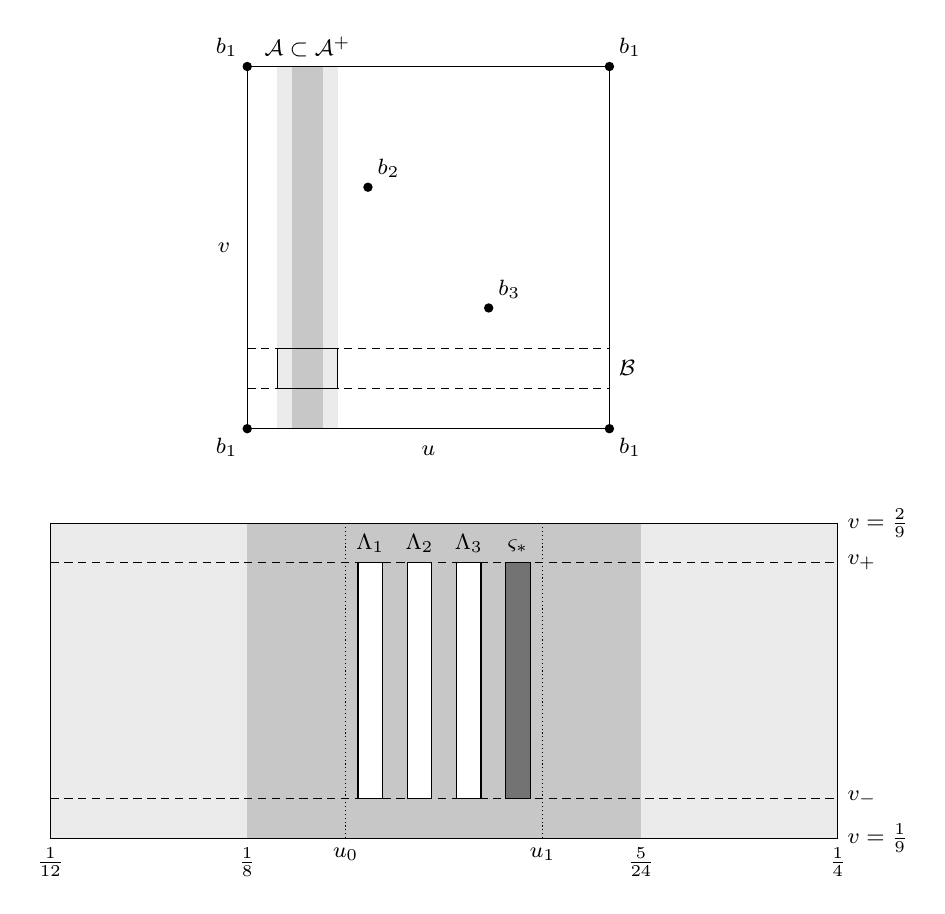
\begin{tikzpicture}[font=\footnotesize]
 \begin{scope}[scale=4.6]
  \fill[black!8] (1/12,0) rectangle (1/4,1);
  \fill[black!22] (1/8,0) rectangle (5/24,1);
  \draw[densely dashed] (0,1/9) -- (1,1/9);
  \draw[densely dashed] (0,2/9) -- (1,2/9);
  \draw (0,0) rectangle (1,1);
  \draw[thin] (1/12,1/9) rectangle (1/4,2/9);
  \foreach \p in {(0,0),(1,0),(0,1),(1,1),(1/3,2/3),(2/3,1/3)} \fill \p circle (0.013);
  \node[below left] at (0,0) {$b_1$};
  \node[below right] at (1,0) {$b_1$};
  \node[above left] at (0,1) {$b_1$};
  \node[above right] at (1,1) {$b_1$};
  \node[above right] at (1/3,2/3) {$b_2$};
  \node[above right] at (2/3,1/3) {$b_3$};
  \node[above] at (1/6,1) {$\mathcal A\subset\mathcal A^+$};
  \node[right] at (1,1/6) {$\mathcal B$};
  \node[below] at (1/2,-0.02) {$u$};
  \node[left] at (-0.02,1/2) {$v$};
 \end{scope}
 \begin{scope}[shift={(-2.5,-5.2)},x=60cm,y=36cm,shift={(-1/12,-1/9)}]
  \fill[black!8] (1/12,1/9) rectangle (1/4,2/9);
  \fill[black!22] (1/8,1/9) rectangle (5/24,2/9);
  \draw (1/12,1/9) rectangle (1/4,2/9);
  \draw[densely dashed] (1/12,1/8) -- (1/4,1/8);
  \draw[densely dashed] (1/12,5/24) -- (1/4,5/24);
  \filldraw[fill=white] (0.14844,1/8) rectangle (0.15365,5/24);
  \node[above] at (0.15104,5/24) {$\Lambda_1$};
  \filldraw[fill=white] (0.15885,1/8) rectangle (0.16406,5/24);
  \node[above] at (0.16146,5/24) {$\Lambda_2$};
  \filldraw[fill=white] (0.16927,1/8) rectangle (0.17448,5/24);
  \node[above] at (0.17188,5/24) {$\Lambda_3$};
  \filldraw[fill=black!55] (0.17969,1/8) rectangle (0.18490,5/24);
  \node[above] at (0.18229,5/24) {$\varsigma_*$};
  \draw[densely dotted] (7/48,1/9) -- (7/48,2/9);
  \draw[densely dotted] (3/16,1/9) -- (3/16,2/9);
  \node[below] at (7/48,1/9) {$u_0$};
  \node[below] at (3/16,1/9) {$u_1$};
  \node[below] at (1/8,1/9) {$\frac18$};
  \node[below] at (5/24,1/9) {$\frac5{24}$};
  \node[below] at (1/12,1/9) {$\frac1{12}$};
  \node[below] at (1/4,1/9) {$\frac14$};
  \node[right] at (1/4,1/8) {$v_-$};
  \node[right] at (1/4,5/24) {$v_+$};
  \node[right] at (1/4,1/9) {$v=\frac19$};
  \node[right] at (1/4,2/9) {$v=\frac29$};
 \end{scope}
\end{tikzpicture}
\caption{The handle data on the base torus $\Gamma=(\R/\Z)^2$ in the coordinates $(u,v)$ (Proposition~\ref{prop:cub-handle},
Definition~\ref{def:shd4-frame}). Top: the annuli $\mathcal A\subset\mathcal A^+$ (dark and light grey), the dual band
$\mathcal B$ (between $v=\frac19$ and $v=\frac29$, dashed) and the marked points $b_1,b_2,b_3$, where $Z_0=0$. Bottom: $\mathcal A^+\cap\mathcal B$
enlarged, dashed at $v=v_\pm$; the clock $f$ rises on $[u_0,u_1]$; the layers $\Lambda_i$ (white) and the
residual layer where $\varsigma_*$ rises (black) lie over $(l_j,r_j)\times(v_-,v_+)$, where $b>0$. Here $k=3$.}
\label{fig:shd4-handle}
\end{figure}

\begin{lemma}[The first path in the frame]\label{lem:shd4-frame-forms}
\lean{SymplecticPacking.Handle.Cubic.OmegaT_frameA, SymplecticPacking.Handle.Cubic.OmegaT_one_frameA,
SymplecticPacking.Handle.Cubic.Omega1Loc}
Over $\mathcal A^+$, $\chi_{\mathcal A}^*\Omega_t=\omega_V+\kappa_t+dp\wedge(a_{\mathcal A}+t\,\partial_p\alpha_1)$ with the positive forms
$\kappa_t$ of Lemma~\ref{lem:fer-positivity}. Over $\mathcal A$,
\[
 \chi_{\mathcal A}^*\Omega_1=\omega_V+e_h\nu+d\bigl(f(u)H^*(p)\beta\bigr).
\]
\end{lemma}

\begin{proof}
Lemma~\ref{lem:fer-positivity} in the frame of Lemma~\ref{lem:fer-frame}, and Lemma~\ref{lem:fer-alpha1}(ii) with $d\Gamma_{\rm sm}=e_h\nu$.
\end{proof}

\emph{The twist.} For $\lambda\in\R$ define on $\mathcal A\times\C$
\begin{equation}\label{eq:shd4-twist}
\begin{gathered}
 \mathcal D_\lambda(u,v,w_{\mathcal A})=\bigl(u,v,q_{\lambda f(u)}(w_{\mathcal A})\bigr),\qquad
 \mathcal D_\lambda^{-1}(u,v,w_{\mathcal A})=\bigl(u,v,q^{-1}_{\lambda f(u)}(w_{\mathcal A})\bigr),\\
 Q^\lambda_u=\lambda f'(u)\,Q_{\lambda f(u)},\qquad G_\lambda(u,w_{\mathcal A})=f(u)\,H^*\bigl(p(q_\lambda^{-1}w_{\mathcal A})\bigr),
\end{gathered}
\end{equation}
and $\mathcal D=\mathcal D_1$; these are smooth in $(\lambda,u,v,w_{\mathcal A})$, mutually inverse, fix base points and preserve $\mathcal A\times D(c)$ for $c>P_{\rm supp}$.
\lean{SymplecticPacking.Handle.Cubic.Dlam, SymplecticPacking.Handle.Cubic.DlamInv, SymplecticPacking.Handle.Cubic.Qs,
SymplecticPacking.Handle.Cubic.Glam}

\begin{lemma}[Suspension]\label{lem:shd4-suspension}
\lean{SymplecticPacking.Handle.Cubic.suspension}
On $\mathcal A\times\C$, $\mathcal D_\lambda^*\omega_V=\omega_V+d\bigl[(Q^\lambda_u\circ q_{\lambda f(u)})\,du\bigr]$ for every $\lambda$.
\end{lemma}

\begin{proof}
\Mref{Lemma}{lem:hdl-suspension}(i) with $m=1$ and $u$ for $s$: $D\mathcal D_\lambda$ fixes $\partial_v$, maps vertical $\xi$ to $Dq\,\xi$ and $\partial_u$ to $\partial_u+X_{Q^\lambda_u}$, and $q_{\lambda f(u)}$ is symplectic.
\end{proof}

\emph{Periodisation.} For a one-form $\alpha$ on $\widetilde N$ supported over $\{u_0\le u\le u_1\}$ put $\operatorname{per}(\alpha)=\sum_{m\in\Z}(T_u^m)^*\alpha$ (locally finite). It is $T_u$-invariant, equals $\alpha$ over $\{u_1-1<u<1+u_0\}$, vanishes near points with $u\notin[u_0,u_1]+\Z$, and for horizontal $\alpha$ its value at a point with $\lfloor u\rfloor=m$ is the covector of $\alpha$ at $T_u^{-m}$ of that point.
\lean{SymplecticPacking.Handle.Ush, SymplecticPacking.Handle.perJ}

\begin{construction}[The second-path primitive]\label{cons:shd4-eta}
\lean{SymplecticPacking.Handle.Cubic.etaLoc, SymplecticPacking.Handle.Cubic.eta, SymplecticPacking.Handle.Cubic.etaPer,
SymplecticPacking.Handle.Cubic.etaDot, SymplecticPacking.Handle.Cubic.OmS1}
On $\mathcal A\times\C$ let
\[
 \upsilon^{\mathcal A}_\lambda=\bigl(Q^\lambda_u\circ q_{\lambda f(u)}\bigr)\,du
 +f(u)\Bigl[H^*\bigl(p(q_\lambda^{-1}q_{\lambda f(u)}w_{\mathcal A})\bigr)-H^*\bigl(p(w_{\mathcal A})\bigr)\Bigr]\beta .
\]
Let $\upsilon_\lambda$ be the one-form on $\widetilde N$ equal to $(\chi_{\mathcal A}^{-1})^*\upsilon^{\mathcal A}_\lambda$ over $\mathcal A$ and to zero
elsewhere, let $\upsilon^{\rm per}_\lambda=\operatorname{per}(\upsilon_\lambda)$, and put
\[
 \Omega^{(1)}_\lambda=\Omega_1+d\upsilon^{\rm per}_\lambda,\qquad \dot\upsilon_\lambda=\partial_\lambda\upsilon^{\rm per}_\lambda .
\]
\end{construction}

\begin{lemma}[Properties of the second-path primitive]\label{lem:shd4-eta}
\lean{SymplecticPacking.Handle.Cubic.etaLoc_eq_zero_of_s, SymplecticPacking.Handle.Cubic.etaLoc_eq_zero_of_p,
SymplecticPacking.Handle.Cubic.eta_support, SymplecticPacking.Handle.Cubic.eta_smooth, SymplecticPacking.Handle.Cubic.eta_zero,
SymplecticPacking.Handle.Cubic.eta_horizontal, SymplecticPacking.Handle.Cubic.eta_TvE, SymplecticPacking.Handle.Cubic.etaDot_far,
SymplecticPacking.Handle.Cubic.firstStage_eq_pre}
\begin{enumerate}[label=(\alph*)]
\item $\upsilon^{\mathcal A}_\lambda$ vanishes for $u\le u_0$, for $u\ge u_1$, and for $p>P_{\rm supp}$; $\upsilon^{\mathcal A}_0=0$.
\item $\upsilon_\lambda$ and $\upsilon^{\rm per}_\lambda$ are horizontal one-forms on $\widetilde N$, smooth in $(\lambda,x)$; $\upsilon_\lambda$ is
$T_v$-invariant, $\upsilon^{\rm per}_\lambda$ is invariant under all deck maps, and $\upsilon^{\rm per}_0=0$. Both $\upsilon^{\rm per}_\lambda$ and $\dot\upsilon_\lambda$ vanish near every point with $p>P_{\rm supp}$ or with
$u\notin[u_0,u_1]+\Z$.
\item Over $\mathcal A$,
$\chi_{\mathcal A}^*\Omega^{(1)}_\lambda=\mathcal D_\lambda^*\bigl(\omega_V+e_h\nu+d(G_\lambda\beta)\bigr)$.
\end{enumerate}
\end{lemma}

\begin{proof}
(a) For $u\le u_0$, $f=f'=0$; for $u\ge u_1$, $f'=0$ and $q_\lambda^{-1}q_{\lambda f(u)}=\mathrm{id}$; for $p>P_{\rm supp}$, $Q_t=0$ near $w_{\mathcal A}$ and $q_t^{\pm1}$ fix it; at $\lambda=0$ both terms vanish.
(b) By (a) the extension by zero is smooth, and horizontal since $\chi_{\mathcal A}$ preserves base points. Its coefficients are $1$-periodic in $v$, so $T_v^*\upsilon_\lambda=\upsilon_\lambda$ by the $T_v$-equivariance of $\chi_{\mathcal A}$; $\operatorname{per}$ gives $T_u$-invariance, preserving $T_v$-invariance as $T_u,T_v$ commute. Supports follow from (a) and the properties of $\operatorname{per}$, also for $\partial_\lambda$.
(c) Over $\mathcal A$, $\upsilon^{\rm per}_\lambda=\upsilon_\lambda$, $\mathcal D_\lambda$ preserves $\nu,\beta$ and $G_\lambda\circ\mathcal D_\lambda=f(u)H^*(p(q_\lambda^{-1}q_{\lambda f(u)}w_{\mathcal A}))$; add Lemma~\ref{lem:shd4-suspension} to Lemma~\ref{lem:shd4-frame-forms}.
\end{proof}

\begin{proposition}[The second path]\label{prop:shd4-second}
\lean{SymplecticPacking.Handle.Cubic.OmegaPreG_split, SymplecticPacking.Handle.Cubic.firstStage_nondeg,
SymplecticPacking.Handle.Cubic.OmS1_preserves, SymplecticPacking.Handle.Cubic.twist_bound,
SymplecticPacking.Handle.Cubic.Hstar_twist_nonneg}
For valid cubic data and $\lambda\in[0,1]$, the form $\Omega^{(1)}_\lambda$ is closed, invariant under all deck maps, equal to
$\Omega_1$ for $\lambda=0$, and nondegenerate at every point of $\{p<h+2\delta_m\}$.
\end{proposition}

\begin{proof}
Closedness, invariance and $\Omega^{(1)}_0=\Omega_1$ follow from Lemma~\ref{lem:shd4-eta}(b) and Lemma~\ref{lem:fer-positivity}. By invariance we check nondegeneracy over $\{u_1-1<u<1+u_0\}$. Near $u\notin[u_0,u_1]$ the form is $\Omega_1$, symplectic on $\{p<\frac13-e_h/9\}\supset\{p<h+2\delta_m\}$ (Lemmas~\ref{lem:fer-positivity}, \ref{lem:shd4-budget}(d)). Over $\mathcal A$, Lemma~\ref{lem:shd4-eta}(c) and \Mref{Lemma}{lem:hdl-top-power}(b) ($n=2$, $\sigma_{\mathcal A}=\nu$, $e=e_h$) give $(\omega_V+e_h\nu+d(G_\lambda\beta))^2=2(e_h+b(v)\,\partial_uG_\lambda)\,\omega_V\wedge\nu$ with $\partial_uG_\lambda(u,w')=f'(u)H^*(p(q_\lambda^{-1}w'))$. If $p(w_{\mathcal A})<h+2\delta_m$, then $w'=q_{\lambda f(u)}(w_{\mathcal A})$ and $q_\lambda^{-1}w'$ lie in $D(h+2\delta_m)$, where $H^*>0$ (Lemma~\ref{lem:shd4-budget}(d)); with $f',b\ge0$, $e_h>0$ the coefficient is positive.
\end{proof}

\emph{The final coefficient.} Put
$G_{\rm f}(u,w)=J(p(w))+\sum_{i=1}^k\varsigma_i(u)\,h_i(p(w))+\varsigma_*(u)\,R^*(w)$ and $A_i=J+\sum_{j<i}h_j$.
\lean{SymplecticPacking.Handle.Cubic.Gf, SymplecticPacking.Handle.Cubic.aLayer}

\begin{lemma}[The final coefficient]\label{lem:shd4-Gf}
\lean{SymplecticPacking.Handle.Cubic.contDiff_Gf, SymplecticPacking.Handle.Cubic.Gf_mono, SymplecticPacking.Handle.Cubic.Gf_low,
SymplecticPacking.Handle.Cubic.Gf_up, SymplecticPacking.Handle.Cubic.Gf_layer}
For valid cubic data, $G_{\rm f}$ is smooth on $\R\times\C$ and
\begin{enumerate}[label=(\alph*)]
\item $\partial_uG_{\rm f}=\sum_i\varsigma_i'h_i\circ p+\varsigma_*'R^*\ge0$ at every $(u,w)$ with $R^*(w)\ge0$;
\item $G_{\rm f}=J\circ p$ for $u\le l_1$, and $G_{\rm f}=K\circ p\circ q^{-1}$ for $u\ge r_*$;
\item $G_{\rm f}(u,w)=A_i(p(w))+\varsigma_i(u)h_i(p(w))$ for $l_i<u<r_i$, $1\le i\le k$.
\end{enumerate}
\end{lemma}

\begin{proof}
(a) Differentiate; $h_i>0$ (Lemma~\ref{lem:shd4-budget}(a)), $\varsigma_j'\ge0$. (b) For $u\le l_1$ all clocks vanish; for $u\ge r_*$ all equal one and $J+\sum_ih_i+R^*=K\circ p\circ q^{-1}$. (c) On $(l_i,r_i)$, $\varsigma_j=1$ for $j<i$ and $\varsigma_j=0$ for $j>i$, including $j=*$.
\end{proof}

\begin{construction}[The third-path primitive]\label{cons:shd4-xi}
\lean{SymplecticPacking.Handle.Cubic.Gdiff, SymplecticPacking.Handle.Cubic.xiA, SymplecticPacking.Handle.Cubic.JbE,
SymplecticPacking.Handle.Cubic.xi, SymplecticPacking.Handle.Cubic.xiPer, SymplecticPacking.Handle.Cubic.OmS2,
SymplecticPacking.Handle.Cubic.OmegaFinalPer, SymplecticPacking.Handle.Cubic.Ghat}
On $\mathcal A\times\C$ let $\xi^{\mathcal A}=\bigl((G_{\rm f}-G_1)\circ\mathcal D\bigr)\beta$. Let $\xi$ be the one-form on $\widetilde N$ equal to
$J(p)\beta+(\chi_{\mathcal A}^{-1})^*\bigl(\xi^{\mathcal A}-J(p)\beta\bigr)$ over $\mathcal A$ and to $J(p)\beta$ elsewhere, and put
\[
\begin{gathered}
 \xi^{\rm per}=J(p)\beta+\operatorname{per}\bigl(\xi-J(p)\beta\bigr),\qquad
 \Omega^{(2)}_\tau=\Omega^{(1)}_1+\tau\,d\xi^{\rm per},\\
 \Omega_{\rm fin}=\Omega^{(2)}_1,\qquad \hat G_\tau=(1-\tau)G_1+\tau G_{\rm f}.
\end{gathered}
\]
\end{construction}

\begin{lemma}[Properties of the third-path primitive]\label{lem:shd4-xi}
\lean{SymplecticPacking.Handle.Cubic.xi_collar, SymplecticPacking.Handle.Cubic.xi_smooth,
SymplecticPacking.Handle.Cubic.xi_horizontal, SymplecticPacking.Handle.Cubic.xi_toric_near_boundary,
SymplecticPacking.Handle.Cubic.xi_TvE, SymplecticPacking.Handle.Cubic.xiPer_deck, SymplecticPacking.Handle.Cubic.xiPer_eq_fX,
SymplecticPacking.Handle.Cubic.fX_far, SymplecticPacking.Handle.Cubic.secondStage_eq_on_A,
SymplecticPacking.Handle.Cubic.secondStage_off}
\begin{enumerate}[label=(\alph*)]
\item $\xi^{\mathcal A}=J(p)\beta$ for $u\le u_0$ and for $u\ge u_1$.
\item $\xi^{\rm per}$ is a smooth one-form on $\widetilde N$, invariant under all deck maps, of the form $\Xi\,\beta$ with $\Xi$ smooth; on
$\{p>P_{\rm supp}\}$, $\Xi$ is a function of $(u\bmod1,p)$.
\item Over $\mathcal A$, $\chi_{\mathcal A}^*\Omega^{(2)}_\tau=\mathcal D^*\bigl(\omega_V+e_h\nu+d(\hat G_\tau\beta)\bigr)$; near points with
$u\notin[u_0,u_1]+\Z$, $\Omega^{(2)}_\tau=\Omega_1+\tau J'(p)\,b(v)\,dp\wedge dv$.
\end{enumerate}
\end{lemma}

\begin{proof}
(a) For $u\le u_0$: $\mathcal D=\mathrm{id}$, $G_1=0$, $G_{\rm f}=J\circ p$. For $u\ge u_1>r_*$: $G_1\circ\mathcal D=H^*(p)$, $G_{\rm f}\circ\mathcal D=K(p)$, with difference $J(p)$.

(b) By (a), $\xi-J(p)\beta$ is supported over $[u_0,u_1]$, so $\xi$ and $\xi^{\rm per}$ are smooth multiples of $\beta$ ($\chi_{\mathcal A}$ preserves base points). Invariance follows as in Lemma~\ref{lem:shd4-eta}(b), $J(p)\beta$ being invariant as deck maps preserve $p$ and $v\bmod1$. On $\{p>P_{\rm supp}\}$, $\mathcal D=\mathrm{id}$ and $G_1,G_{\rm f}$ depend only on $(u,p)$.

(c) Over $\mathcal A$, $\chi_{\mathcal A}^*\xi^{\rm per}=\mathcal D^*((G_{\rm f}-G_1)\beta)$; add Lemma~\ref{lem:shd4-eta}(c) at $\lambda=1$. Near $u\notin[u_0,u_1]+\Z$, $\upsilon^{\rm per}_1=0$, $\xi^{\rm per}=J(p)\beta$ and $d(J(p)\beta)=J'(p)b(v)\,dp\wedge dv$.
\end{proof}

\begin{proposition}[The third path and the final form]\label{prop:shd4-third}
\lean{SymplecticPacking.Handle.Cubic.secondStage_nondeg, SymplecticPacking.Handle.Cubic.OmS2_preserves,
SymplecticPacking.Handle.Cubic.OmegaFinalPer_eq, SymplecticPacking.Handle.Cubic.OmegaFinal_eq_pullback,
SymplecticPacking.Strip.Cubic.DinvN, SymplecticPacking.Strip.Cubic.DinvN_pullback}
For valid cubic data and $\tau\in[0,1]$, $\Omega^{(2)}_\tau$ is closed, invariant under all deck maps and nondegenerate at every
point of $\{p<h+2\delta_m\}$. Over $\mathcal A$,
\[
 \chi_{\mathcal A}^*\Omega_{\rm fin}=\mathcal D^*\Omega_{\rm pre},\qquad
 (\chi_{\mathcal A}\circ\mathcal D^{-1})^*\Omega_{\rm fin}=\Omega_{\rm pre},\qquad
 \Omega_{\rm pre}=\omega_V+e_h\nu+d(G_{\rm f}\beta),
\]
and $\chi_{\mathcal A}\circ\mathcal D^{-1}$ maps $\mathcal A\times D(h)$ diffeomorphically onto $\mathcal A\times D(h)$.
\end{proposition}

\begin{proof}
Closedness and invariance follow from Proposition~\ref{prop:shd4-second} and Lemma~\ref{lem:shd4-xi}(b), so it suffices to work over $\{u_1-1<u<1+u_0\}$.

Over $\mathcal A$, Lemma~\ref{lem:shd4-xi}(c) and \Mref{Lemma}{lem:hdl-top-power}(b) give the square at $\mathcal D(x)$ as $2(e_h+b\,\partial_u\hat G_\tau)\,\omega_V\wedge\nu$, where $\partial_u\hat G_\tau=(1-\tau)\partial_uG_1+\tau\partial_uG_{\rm f}$. If $p(x)<h+2\delta_m$, the image fibre point $w'$ has $p(w')<h+2\delta_m$, so $\partial_uG_1(u,w')\ge0$ as in Proposition~\ref{prop:shd4-second}, and $\partial_uG_{\rm f}(u,w')\ge0$ by Lemmas~\ref{lem:shd4-Gf}(a) and~\ref{lem:shd4-budget}(d).

Near $u\notin[u_0,u_1]$, Lemma~\ref{lem:shd4-xi}(c) adds $dp\wedge(\text{base one-form})$ to $\Omega_1$, which changes only the mixed part in the local form of Lemma~\ref{lem:fer-positivity}; the square remains $2\omega_V\wedge\kappa_1>0$ (Lemma~\ref{lem:pre-top-power}).

The identities are Lemma~\ref{lem:shd4-xi}(c) at $\tau=1$. The last claim holds because $\mathcal D^{\pm1}$ fix base points, $q_t^{\pm1}$ preserve $D(h)$, and $\chi_{\mathcal A}$ preserves $p$.
\end{proof}

\begin{lemma}[Vanishing on the marked fibres]\label{lem:shd4-fibres}
\lean{SymplecticPacking.Handle.fibreSetH, SymplecticPacking.Handle.Cubic.alpha1E_fibre,
SymplecticPacking.Handle.Cubic.etaDot_fibre, SymplecticPacking.Handle.Cubic.xiPer_fibre,
SymplecticPacking.Handle.Cubic.xi_zero_of_bB, SymplecticPacking.Handle.Cubic.xiPer_fibre}
Let $\widetilde{\mathcal F}$ be the union of all lifts of the fibres $N_{b_1},N_{b_2},N_{b_3}$, that is, the set of points
$(u,v,w)$ with $(u,v)\in b_j+\Z^2$ for some $j$. At every point of $\widetilde{\mathcal F}$ the covectors $\alpha_1$, $\dot\upsilon_\lambda$ $(\lambda\in\R)$ and $\xi^{\rm per}$ of
$T^*\widetilde N$ are zero.
\end{lemma}

\begin{proof}
For $\alpha_1$, lift Lemma~\ref{lem:fer-alpha1-fibres} to the cover, where $\alpha_1$ is periodic. The $u$-coordinates $0,\frac13,\frac23$ of the $b_j$ avoid $[u_0,u_1]=[\frac7{48},\frac9{48}]$ mod one, so $\dot\upsilon_\lambda$ vanishes near $\widetilde{\mathcal F}$ by Lemma~\ref{lem:shd4-eta}(b). Finally, $\xi^{\rm per}=\Xi\,b(v)\,dv$ by Lemma~\ref{lem:shd4-xi}(b). The $v$-coordinates $0,\frac23,\frac13$ lie outside $[\frac18,\frac5{24}]+\Z\supset\operatorname{supp}b$ (Proposition~\ref{prop:cub-handle}(c)), so $\beta=0$ on $\widetilde{\mathcal F}$.
\end{proof}

\begin{construction}[The handle Moser map]\label{cons:shd4-moser}
\lean{SymplecticPacking.Handle.Cubic.stage0, SymplecticPacking.Handle.Cubic.stage1, SymplecticPacking.Handle.Cubic.stage2,
SymplecticPacking.Handle.clock, SymplecticPacking.Handle.moserPathB, SymplecticPacking.Handle.moserVariationB,
SymplecticPacking.Handle.concat3B, SymplecticPacking.Handle.Cubic.handleData, SymplecticPacking.Handle.Cubic.handleParams,
SymplecticPacking.Handle.solve4, SymplecticPacking.Handle.cutoffChi, SymplecticPacking.Handle.boxFieldP,
SymplecticPacking.Handle.Cubic.handlePhi, SymplecticPacking.Handle.Cubic.handlePhiInv}
The three stages are
\[
 (\Omega^{(0)}_s,\mathfrak v^{(0)}_s)=(\Omega_s,\alpha_1),\qquad
 (\Omega^{(1)}_s,\mathfrak v^{(1)}_s)=(\Omega^{(1)}_s,\dot\upsilon_s),\qquad
 (\Omega^{(2)}_s,\mathfrak v^{(2)}_s)=(\Omega^{(2)}_s,\xi^{\rm per}),
\]
with matching endpoints $\Omega^{(0)}_1=\Omega^{(1)}_0$ and $\Omega^{(1)}_1=\Omega^{(2)}_0$. With the clocks $\sigma_i(t)=S(9t-3i-1)$,
$i=0,1,2$, which move only on $[\frac{3i+1}9,\frac{3i+2}9]$, put
\[
 \Omega^{\rm M}_t=\Omega^{(0)}_{\sigma_0(t)}+\sum_{i=1,2}\bigl(\Omega^{(i)}_{\sigma_i(t)}-\Omega^{(i)}_0\bigr),\qquad
 \mathfrak v_t=\sum_{i=0}^2\sigma_i'(t)\,\mathfrak v^{(i)}_{\sigma_i(t)} .
\]
On $U=\{p<h+2\delta_m\}$ let $Y_t$ be the field with $\iota_{Y_t}\Omega^{\rm M}_t=-\mathfrak v_t$; in the coordinates
$(\operatorname{Re}w,\operatorname{Im}w,u,v)$ it is the adjugate solution of a $4\times4$ skew system. With the moment cutoff
\[
 \mathfrak c(p)=S\Bigl(\frac{h+\frac74\delta_m-p}{\delta_m/4}\Bigr),
\]
which equals one for $p\le h+\frac32\delta_m$ and zero for $p\ge h+\frac74\delta_m$, let $\widehat Y_t=\mathfrak c(p)Y_t$, extended by zero.
The handle Moser map $\Phi$ is the time-one map of $\widehat Y$ from time $0$, and $\Phi^{-1}$ is its inverse.
\end{construction}

\begin{proposition}[The handle Moser map]\label{prop:shd4-moser}
\lean[needed]{SymplecticPacking.Handle.Cubic.handleMoser, SymplecticPacking.Handle.handle_moser_global,
SymplecticPacking.Handle.Cubic.OmegaT_toric, SymplecticPacking.Handle.Cubic.etaDot_far,
SymplecticPacking.Handle.Cubic.d1_xiPer_toric, SymplecticPacking.Handle.Cubic.handleData_pres}
For valid cubic data, $\Phi$ and $\Phi^{-1}$ are mutually inverse $C^\infty$ diffeomorphisms of $\widetilde N$, and:
\begin{enumerate}[label=(\alph*)]
\item $\Phi^*\Omega_{\rm fin}=\Omega_0$ and $(\Phi^{-1})^*\Omega_0=\Omega_{\rm fin}$ at every point of $\{p\le h+\delta_m\}$;
\item for every $c>P_{\rm supp}$, $\Phi$ and $\Phi^{-1}$ map each of $\{p\le c\}$, $\{p<c\}$, $\{p=c\}$ onto itself;
\item $\Phi$ and $\Phi^{-1}$ fix every point of $\widetilde{\mathcal F}$;
\item $\Phi$ and $\Phi^{-1}$ commute with every deck map.
\end{enumerate}
Moreover $\Phi=\Phi_2\circ\Phi_1\circ\Phi_0$, where $\Phi_i$ is the time-one map of the cut stage field $\mathfrak c(p)Y^{(i)}_s$,
$\iota_{Y^{(i)}_s}\Omega^{(i)}_s=-\mathfrak v^{(i)}_s$.
\end{proposition}

\begin{proof}
\emph{Hypotheses.} On $[\frac{3i+1}9,\frac{3i+2}9]$ only $\sigma_i$ moves, so $\Omega^{\rm M}_t=\Omega^{(i)}_{\sigma_i(t)}$ there; $\Omega^{\rm M}_t=\Omega_0$ for $t\le\frac19$ and $\Omega^{\rm M}_t=\Omega_{\rm fin}$ for $t\ge\frac89$. Hence $\Omega^{\rm M}_t$ is closed and nondegenerate on $U$, by Lemma~\ref{lem:fer-positivity}, Lemma~\ref{lem:shd4-budget}(d) and Propositions~\ref{prop:shd4-second},~\ref{prop:shd4-third}.

The pair is smooth on $\R\times\widetilde N$, with $\partial_t\Omega^{\rm M}_t=d\mathfrak v_t$ and $\mathfrak v_t=0$ for $t\notin(0,1)$. By Lemma~\ref{lem:pre-moser}(a), $Y$ is smooth on $\R\times U$, hence $\widehat Y$ is smooth on $\R\times\widetilde N$. All stage data and $\mathfrak c(p)$ are deck invariant.

\emph{Toric band.} Let $R=2\pi(-y\partial_x+x\partial_y)$ with $w=x+iy$, so that $\iota_R\Omega_0=-dp$ (Lemma~\ref{lem:fer-positivity}). On $U'=\{P_{\rm supp}<p<h+2\delta_m\}$ we have $\iota_R\Omega^{\rm M}_t=-dp$ and $\mathfrak v_t(R)=0$: $\alpha_1$ is horizontal with $\iota_Rd\alpha_1=0$, $\upsilon^{\rm per}_s$ and $\dot\upsilon_s$ vanish near $U'$ (Lemma~\ref{lem:shd4-eta}(b)), and $\xi^{\rm per}=\Xi(u\bmod1,p)\,b(v)\,dv$ on $U'$. Lemma~\ref{lem:pre-moser}(d) then gives $dp(\widehat Y_t)=0$ on $\{p>P_{\rm supp}\}$. Moreover $\widehat Y=0$ for $p\ge h+\frac74\delta_m$.

\emph{Completeness.} By Lemma~\ref{lem:pre-moser}(g), $du(\widehat Y_t)$ and $dv(\widehat Y_t)$ are deck invariant, hence $|du(\widehat Y_t)|+|dv(\widehat Y_t)|\le C_b$, the maximum over $[0,1]\times[0,1]^2\times\bar D(h+\frac74\delta_m)$; also $\widehat Y_t=0$ for $t\notin[0,1]$. By the toric band, an integral curve through $x$ stays in $\{p\le\max(p(x),h)\}$ with base displacement at most $C_b$, so the flow is global and smooth.

\emph{Conclusions.}
(b) follows from $dp(\widehat Y_t)=0$ on $\{p>P_{\rm supp}\}$.
(a) Since $P_{\rm supp}<h$, curves from $\{p\le h+\delta_m\}$ stay there, and $\{p<h+\frac32\delta_m\}$ is invariant. There $\mathfrak c=1$, so Lemma~\ref{lem:pre-moser}(b) gives $(\Phi^*\Omega^{\rm M}_1)_x=(\Omega^{\rm M}_0)_x$; the inverse identity follows as $\Phi^{-1}$ preserves $\{p\le h+\delta_m\}$.
(c) By Lemma~\ref{lem:shd4-fibres}, $\widehat Y_t=0$ on $\widetilde{\mathcal F}$; apply Lemma~\ref{lem:pre-moser}(c).
(d) is Lemma~\ref{lem:pre-moser}(g).

\emph{Decomposition.} Each stage pair is deck invariant and satisfies $\iota_R\Omega^{(i)}_s=-dp$ and $\mathfrak v^{(i)}_s(R)=0$ on $U'$, so the same argument gives a global flow $\Phi^{(i)}_s$ of $\mathfrak c(p)Y^{(i)}_s$; set $\Phi_i=\Phi^{(i)}_1$. On $[\frac{3i+1}9,\frac{3i+2}9]$ we have $\widehat Y_t=\sigma_i'(t)\mathfrak c(p)Y^{(i)}_{\sigma_i(t)}$, so $t\mapsto\Phi^{(i)}_{\sigma_i(t)}(x)$ is an integral curve of $\widehat Y$; elsewhere $\widehat Y_t=0$. Uniqueness and Lemma~\ref{lem:pre-moser}(f) give $\Phi=\Phi_2\circ\Phi_1\circ\Phi_0$.
\end{proof}

Equivalently, let $\Phi_A$ ($A\ge0$) be the time-one map of $\widehat Y$ times a product cutoff in $(u,v)$ equal to one on $\{|u|,|v|\le A+C_b+2\}$. Then $\Phi(x)=\Phi_A(x)$ for $A=|u(x)|+|v(x)|$, by the base speed bound.
\lean{SymplecticPacking.Handle.boxCut, SymplecticPacking.Handle.Cb, SymplecticPacking.Handle.boxL,
SymplecticPacking.Handle.PhiB, SymplecticPacking.Handle.PhiG, SymplecticPacking.Handle.PhiGInv,
SymplecticPacking.Handle.lfield_boxField, SymplecticPacking.Handle.LField.flowFrom_isSol, SymplecticPacking.Handle.flowFrom_box_eq}

\emph{Layer maps.} Work on the layer $\Lambda_i=\{l_i<u<r_i,\ \frac18<v<\frac5{24},\ p<h\}$ (frame coordinates). Let $T(v)=\int_{1/8}^vb$, a diffeomorphism $(\frac18,\frac5{24})\to(0,1)$ with $dT=\beta$ and inverse $v(T)$. Set $\ell(T)=e_h/b(v(T))$ and
\[
 x_i(u,T,p)=(u-l_i)\,\ell(T)+\varsigma_i(u)\,h_i(p).
\]
Since $\partial_ux_i=\ell+\varsigma_i'h_i>0$, $x_i=0$ at $u=l_i$ and $x_i>h_i(p)$ at $u=r_i$, there is a unique root $u=\sigma_i(x,T,p)\in(l_i,r_i)$ for $0<x<h_i(p)$, $0<T<1$.

For $1\le i\le k$ put $\bar\rho_i=(\rho_i+a_i)/2$, $\delta_i=a_i-\bar\rho_i$ and $\hat\rho_i=\bar\rho_i+\delta_i/4$. For $(z_{\rm b},z_{\rm f})\in\Bo(\hat\rho_i)\subset\C^2$, write $(x,T)=\Psi_{\delta_i}(z_{\rm b})$ (Proposition~\ref{prop:hdl-strip}) and $p=\pi|z_{\rm f}|^2$, and define
\[
 E_i(z_{\rm b},z_{\rm f})=\Bigl(\sigma_i(x,T,p),\ v(T),\ e^{-2\pi iTA_i'(p)}z_{\rm f}\Bigr),\qquad
 f^N_i=\Phi^{-1}\circ\chi_{\mathcal A}\circ\mathcal D^{-1}\circ E_i .
\]
\lean{SymplecticPacking.Strip.Cubic.ell, SymplecticPacking.Strip.Cubic.layerX, SymplecticPacking.Strip.Cubic.layerRoot,
SymplecticPacking.Strip.Cubic.shear, SymplecticPacking.Strip.Cubic.srcMap, SymplecticPacking.Strip.Cubic.layerMap,
SymplecticPacking.Strip.Cubic.layerMap_eq, SymplecticPacking.Strip.Cubic.fN}

\begin{proposition}[The four-dimensional embeddings into the cover]\label{prop:shd4-maps}
\lean[needed]{SymplecticPacking.Strip.Cubic.x_lt_hi, SymplecticPacking.Strip.Cubic.layer_form,
SymplecticPacking.Strip.Cubic.shear_pullback, SymplecticPacking.Strip.Cubic.layerMap_symplectic,
SymplecticPacking.Strip.Cubic.layerMap_mem_annulus, SymplecticPacking.Strip.Cubic.layerMap_injective,
SymplecticPacking.Strip.Cubic.layerMap_disjoint, SymplecticPacking.Strip.Cubic.layerMap_compact,
SymplecticPacking.Strip.Cubic.fN_mem, SymplecticPacking.Strip.Cubic.fN_smooth, SymplecticPacking.Strip.Cubic.fN_symplectic,
SymplecticPacking.Strip.Cubic.fN_eq_imp, SymplecticPacking.Strip.Cubic.fN_disjoint,
SymplecticPacking.Strip.Cubic.fN_avoid_fibres, SymplecticPacking.Strip.Cubic.fN_eq_imp,
SymplecticPacking.Embed.Cubic.fcap_eq_imp}
Let the cubic data be valid and $1\le i,j\le k$. Then $\rho_i<\bar\rho_i<\hat\rho_i<a_i$, and:
\begin{enumerate}[label=(\alph*)]
\item $f^N_i$ is defined and smooth on $\Bo(\hat\rho_i)$, with values in $\{p<h\}\setminus\widetilde{\mathcal F}$, and
$(f^N_i)^*\Omega_0=\omega_0$;
\item $f^N_i$ is injective, $f^N_i(\Bo(\hat\rho_i))\cap f^N_j(\Bo(\hat\rho_j))=\varnothing$ for $i\ne j$, and $f^N_i(B(\bar\rho_i))$ is compact;
\item if $f^N_i(X)=T\,f^N_j(X')$ for a deck map $T$, then $T=\mathrm{id}$, $i=j$ and $X=X'$.
\end{enumerate}
\end{proposition}

\begin{proof}
Let $\varpi=\pi|z_{\rm b}|^2$, so $\varpi+p<\hat\rho_i$. By Proposition~\ref{prop:hdl-strip} and Lemma~\ref{lem:shd4-budget}(a),
\[
0<x<\varpi+\tfrac{\delta_i}2<a_i-p-\tfrac{\delta_i}4<h_i(p),\qquad p<a_i<h,
\]
so $E_i$ maps $\Bo(\hat\rho_i)$ into $\Lambda_i$.

Since $\ell\,b=e_h$, $e_h\nu=\ell\,du\wedge dT$, and by Lemma~\ref{lem:shd4-Gf}(c), $d(G_{\rm f}\beta)=(\varsigma_i'h_i\,du+dA_i+\varsigma_i\,dh_i)\wedge dT$ on $\Lambda_i$; hence $\Omega_{\rm pre}=\omega_V+dx_i\wedge dT+dA_i(p)\wedge dT$ there.

Now $E_i$ is the composite of $\Psi_{\delta_i}\times\mathrm{id}$, the shear of Lemma~\ref{lem:hdl-shear} with $A=A_i$, and the inverse of $(u,v,w_{\mathcal A})\mapsto(x_i,T,w_{\mathcal A})$ (the periodic counterpart of the layer maps of~\cite{SongHD}). By Proposition~\ref{prop:hdl-strip} and Lemma~\ref{lem:hdl-shear}, $E_i$ is a diffeomorphism onto an open subset of $\Lambda_i$ with $E_i^*\Omega_{\rm pre}=\omega_0$.

(a) By Proposition~\ref{prop:shd4-third}, $\chi_{\mathcal A}\mathcal D^{-1}$ maps $\Lambda_i$ into $\mathcal A\times D(h)$ and pulls $\Omega_{\rm fin}$ back to $\Omega_{\rm pre}$; by Proposition~\ref{prop:shd4-moser}(a),(b), $\Phi^{-1}$ preserves $\{p<h\}$ and pulls $\Omega_0$ back to $\Omega_{\rm fin}$ there. Composing gives $(f^N_i)^*\Omega_0=\omega_0$. The point $\chi_{\mathcal A}\mathcal D^{-1}E_i(X)$ lies over $\mathcal A$, which misses $\widetilde{\mathcal F}$, and $\Phi^{\pm1}$ fix $\widetilde{\mathcal F}$ pointwise (Proposition~\ref{prop:shd4-moser}(c)), so $f^N_i$ misses $\widetilde{\mathcal F}$.

(b) $E_i$ is injective, and the images of different $E_i$ lie over the disjoint intervals $(l_i,r_i)$. The maps $\chi_{\mathcal A}\mathcal D^{-1}$ and $\Phi^{-1}$ are injective and common to all $i$. The closed ball is compact.

(c) By Proposition~\ref{prop:shd4-moser}(d), $y=\chi_{\mathcal A}\mathcal D^{-1}E_i(X)$ and $y'=\chi_{\mathcal A}\mathcal D^{-1}E_j(X')$ satisfy $y=Ty'$. Both lie over $(\frac18,\frac5{24})^2$, so $T=\mathrm{id}$, and (b) gives $i=j$ and $X=X'$.
\end{proof}

\begin{remark}[The four-dimensional embeddings]\label{rem:shd-four}
\lean{SymplecticPacking.Embed.Cubic.fcap, SymplecticPacking.Embed.Cubic.fcapV, SymplecticPacking.Branch2.CubicData.fcapGen,
SymplecticPacking.Handle.Cubic.handleMoser, SymplecticPacking.Strip.fN, SymplecticPacking.Embed.Cubic.fcap,
SymplecticPacking.Branch2.embeddings2, SymplecticPacking.Branch2.embeddingsEq, SymplecticPacking.Branch2.CubicData.ofParams}
By Proposition~\ref{prop:shd4-maps}(a),(c) the maps $f^N_i$ satisfy the hypotheses of Theorem~\ref{thm:cub-transfer}, and
the four-dimensional embeddings are
$f^{\rm cap}_i=b_{\rm ball}\circ\mathcal T_{\rm u}\circ\mathsf N\circ f^N_i$ on $\Bo(\hat\rho_i)$. The equal branch uses these maps for the data of
Remark~\ref{rem:rtc-equal}: $\rho_i=\rho$, $a_i=a$, $K(p)=(3\sqrt k-9)p$, and $(q_t)$ the isotopy of
Theorem~\ref{thm:pll-inner}, with the recorded capacities of Remark~\ref{rem:rtc-recorded}; the valid cubic data
of~\cite{SongHD} use the same maps. The strip constants are
the four-dimensional values of Definition~\ref{def:str-enlarged}; only the disc-to-strip map of Proposition~\ref{prop:str-strip}
is taken from \S\ref{sec:str}.
\end{remark}

\subsection{The shear and the strip map}\label{sec:shd-shear}

The layer maps of \S\ref{sec:shd-four}, and those of the higher-dimensional handle~\cite{SongHD}, use the
following two maps.

\begin{lemma}[Multi-angle shear]\label{lem:hdl-shear}
\lean{OAI.PackingSufficiencySupport.Hamiltonian.toricSuspension,
OAI.PackingSufficiencySupport.Hamiltonian.toricSuspensionInverse_smooth,
OAI.PackingSufficiencySupport.Hamiltonian.toricSuspension_pullback,
OAI.PackingSufficiencySupport.Hamiltonian.toricSuspensionInverse_left,
OAI.PackingSufficiencySupport.Hamiltonian.toricSuspensionInverse_right}
Let $A$ be a smooth function on an open set $W\subset\R^m$ and $\mathrm{Sh}_A(x,T,w)=(x,T,\mathrm{Sh}_{A,T}(w))$, where
\[
 \mathrm{Sh}_{A,T}(w)_j=\exp\big(-2\pi i\,T\,\partial_jA(p(w))\big)\,w_j\qquad(1\le j\le m),
\]
on $\{(x,T,w):p(w)\in W\}\subset\R^2\times\C^m$. Then $\mathrm{Sh}_A$ is a diffeomorphism of this set onto itself, preserves
$p$, $x$ and $T$, and
\[
 \mathrm{Sh}_A^*\big(\omega_V+dx\wedge dT+dA(p)\wedge dT\big)=\omega_V+dx\wedge dT .
\]
\end{lemma}

\begin{proof}
$\mathrm{Sh}_{A,T}$ multiplies each $w_j$ by a unimodular factor smooth in $(T,p(w))$, so it preserves $p$; the same formula with $+2\pi i$ is a smooth inverse, also on the coordinate axes. Where all $w_j\ne0$, write $w_j=\sqrt{p_j/\pi}\,e^{2\pi i\theta_j}$; then $\mathrm{Sh}_{A,T}$ is $\theta_j\mapsto\theta_j-T\partial_jA(p)$ and
\[
\mathrm{Sh}_A^*\omega_V=\omega_V-dA\wedge dT-T\sum_{j,k}\partial_{jk}A\,dp_j\wedge dp_k=\omega_V-dA\wedge dT .
\]
The Hessian term vanishes by symmetry, and $dx\wedge dT$ and $dA(p)\wedge dT$ are unchanged. The identity extends to the axes by continuity.
\end{proof}

\begin{proposition}[Disc-to-strip map]\label{prop:hdl-strip}
\lean{SymplecticPacking.Strip.psiStrip, SymplecticPacking.Strip.psiStrip_smooth,
 SymplecticPacking.Strip.psiStrip_symplectic, SymplecticPacking.Strip.psiStrip_bijOn,
 SymplecticPacking.Strip.psiStrip_x_pos, SymplecticPacking.Strip.psiStrip_x_lt}
\uses{prop:str-strip}
For every $\delta>0$ there is an explicit smooth diffeomorphism
$\Psi_\delta\colon\C\to(0,\infty)\times(0,1)$, $z\mapsto(x,T)$, with $\Psi_\delta^*(dx\wedge dT)=\omega_\C$ and
\[
 0<x<\pi|z|^2+\frac\delta2\qquad\text{for all }z\in\C .
\]
\end{proposition}

The map is $\Psi_\delta=F\circ\mathsf T^{-1}\circ\mathsf D$, with $\varepsilon=\delta/\pi$: $F(u,v)=(X(u),Y(v))$ inverts the square roots of the Morse functions $x+\varepsilon^2/(4x)-\varepsilon$ on $(0,\infty)$ and $\varepsilon\,[(2\sqrt{T(1-T)})^{-1}-1]$ on $(0,1)$, and $\mathsf T$, $\mathsf D$ are the explicit rotation and radial area normalisations of the density $X'(u)Y'(v)$. The estimate holds because the level set of energy $\mathcal E$ encloses area at least $\mathcal E-\varepsilon(\frac\pi2-1)$ and lies in $\{x<\mathcal E+\varepsilon\}$ (Proposition~\ref{prop:str-strip}). Some excess is unavoidable, since no area-preserving map takes the closed disc of area $a$ into $\{0<x<a\}\times(0,1)$; the excess $\delta/2$ serves all concentric discs at once.

\section{The disc-to-strip map and the layer maps}\label{sec:str}

This section constructs the planar disc-to-strip map and proves Proposition~\ref{prop:hdl-strip}. The higher-dimensional layer maps, one ball per layer, are in~\cite{SongHD}.

\medskip\noindent\emph{Conventions.}
On $\C\ni z=x+iy$, $\omega_\C=dx\wedge dy=dI\wedge d\theta$ with $I=\pi|z|^2$, $\theta=\arg z/2\pi$. The strip $(0,\infty)\times(0,1)$ has coordinates $(x,T)$ and area form $dx\wedge dT$. The plane $\R^2\ni\xi=(\xi_1,\xi_2)\cong\C$ ($\xi\mapsto\xi_1+i\xi_2$) carries $d\xi=d\xi_1\wedge d\xi_2$; $\mathrm{Rot}_\phi$ is rotation by $\phi$. In \S\ref{sec:str-balls} (and~\cite{SongHD}) $\C^n=\C\times\C^m\ni(z_{\rm b},z_{\rm f})$, $\varpi=\pi|z_{\rm b}|^2$, $p=p(z_{\rm f})$, so $\omega_0=\omega_\C(z_{\rm b})+\omega_V(z_{\rm f})$, $B(c)=\{\varpi+|p|\le c\}$, $\Bo(c)=\{\varpi+|p|<c\}$.

\subsection{The strip Morse functions}\label{sec:str-morse}

$\Psi_\delta$ sends the circle of area $I$ onto a level set of $R_{\rm st}(x)+V_{\rm st}(T)$ inside $\{x<I+\frac\delta2\}$ (Figure~\ref{fig:str-strip}); it is the product $F_{\rm st}$ of signed square-root inverses $X_{\rm st},Y_{\rm st}$ of $R_{\rm st},V_{\rm st}$, followed by two circle-preserving density normalisations.

\begin{construction}[Strip Morse functions]\label{cons:str-morse}
\lean{SymplecticPacking.Strip.bst, SymplecticPacking.Strip.Rst, SymplecticPacking.Strip.Vst,
SymplecticPacking.Strip.Xst, SymplecticPacking.Strip.Yst, SymplecticPacking.Strip.Jst}
Let $\delta>0$ and $b_{\rm st}=\delta/\pi$. For $x>0$, $0<T<1$ and $\xi=(\xi_1,\xi_2)\in\R^2$ put
\begin{align*}
 R_{\rm st}(x)&=x+\frac{b_{\rm st}^2}{4x}-b_{\rm st}, &
 V_{\rm st}(T)&=b_{\rm st}\Big[\frac{1}{2\sqrt{T(1-T)}}-1\Big],\\
 X_{\rm st}(\xi_1)&=\tfrac12\Big[\xi_1^2+b_{\rm st}+\xi_1\sqrt{\xi_1^2+2b_{\rm st}}\Big], &
 Y_{\rm st}(\xi_2)&=\frac12+\frac{\xi_2\sqrt{\xi_2^2+2b_{\rm st}}}{2(\xi_2^2+b_{\rm st})} ,
\end{align*}
and $F_{\rm st}(\xi)=\big(X_{\rm st}(\xi_1),Y_{\rm st}(\xi_2)\big)$, $\mathcal J_{\rm st}(\xi)=X_{\rm st}'(\xi_1)\,Y_{\rm st}'(\xi_2)$.
\end{construction}

\begin{lemma}[Smooth Morse inverses]\label{lem:str-morse-inverse}
\lean{SymplecticPacking.Strip.Rst_nonneg, SymplecticPacking.Strip.Rst_eq_zero_iff,
 SymplecticPacking.Strip.Vst_nonneg, SymplecticPacking.Strip.Vst_eq_zero_iff,
 SymplecticPacking.Strip.Rst_Xst, SymplecticPacking.Strip.Vst_Yst,
 SymplecticPacking.Strip.deriv_Xst, SymplecticPacking.Strip.deriv_Yst,
 SymplecticPacking.Strip.contDiff_Xst, SymplecticPacking.Strip.contDiff_Yst,
 SymplecticPacking.Strip.Xst_bijOn, SymplecticPacking.Strip.Yst_bijOn}
\uses{cons:str-morse}
\begin{enumerate}[label=(\roman*)]
\item $R_{\rm st}\ge0$ on $(0,\infty)$ with unique zero $x=b_{\rm st}/2$, and $V_{\rm st}\ge0$ on $(0,1)$ with unique zero
$T=\frac12$.
\item $R_{\rm st}(X_{\rm st}(\xi_1))=\xi_1^2$ and $V_{\rm st}(Y_{\rm st}(\xi_2))=\xi_2^2$ for all $\xi_1,\xi_2\in\R$.
\item $X_{\rm st}$ and $Y_{\rm st}$ are smooth on $\R$, with
\[
 X_{\rm st}'(\xi_1)=\frac{\big(\xi_1+\sqrt{\xi_1^2+2b_{\rm st}}\big)^2}{2\sqrt{\xi_1^2+2b_{\rm st}}}>0,\qquad
 Y_{\rm st}'(\xi_2)=\frac{b_{\rm st}^2}{\sqrt{\xi_2^2+2b_{\rm st}}\,(\xi_2^2+b_{\rm st})^2}>0 .
\]
\item $X_{\rm st}$ is an increasing bijection $\R\to(0,\infty)$ and $Y_{\rm st}$ an increasing bijection $\R\to(0,1)$.
$F_{\rm st}$ is a smooth diffeomorphism of $\R^2$ onto $(0,\infty)\times(0,1)$ with
$F_{\rm st}^*(dx\wedge dT)=\mathcal J_{\rm st}\,d\xi$ and $R_{\rm st}\circ X_{\rm st}+V_{\rm st}\circ Y_{\rm st}=|\xi|^2$.
\end{enumerate}
\end{lemma}

\begin{proof}
(i) $R_{\rm st}(x)=(\sqrt x-b_{\rm st}/(2\sqrt x))^2$, which vanishes only at $x=b_{\rm st}/2$. Since $T(1-T)\le\frac14$ with
equality only at $T=\frac12$, $V_{\rm st}\ge0$ with unique zero $T=\frac12$.

(ii) For $x>0$, $R_{\rm st}(x)=\xi_1^2$ is equivalent to $x^2-(\xi_1^2+b_{\rm st})x+b_{\rm st}^2/4=0$, with discriminant
$(\xi_1^2+b_{\rm st})^2-b_{\rm st}^2=\xi_1^2(\xi_1^2+2b_{\rm st})$ and roots
$x_\pm=\frac12[\xi_1^2+b_{\rm st}\pm|\xi_1|\sqrt{\xi_1^2+2b_{\rm st}}]$, both positive because $x_+x_-=b_{\rm st}^2/4$.
$X_{\rm st}(\xi_1)$ is $x_+$ for $\xi_1\ge0$ and $x_-$ for $\xi_1\le0$. For the second identity write $Y_{\rm st}=\frac12+\tau$
with $\tau=\xi_2\sqrt{\xi_2^2+2b_{\rm st}}/(2(\xi_2^2+b_{\rm st}))$. Then
$\tau^2=\frac14-\frac{b_{\rm st}^2}{4(\xi_2^2+b_{\rm st})^2}<\frac14$, so $0<Y_{\rm st}<1$,
$T(1-T)=\frac14-\tau^2=b_{\rm st}^2/(4(\xi_2^2+b_{\rm st})^2)$ for $T=Y_{\rm st}(\xi_2)$, hence
$1/(2\sqrt{T(1-T)})=(\xi_2^2+b_{\rm st})/b_{\rm st}$ and $V_{\rm st}(T)=\xi_2^2$.

(iii) Smoothness holds because $\xi_1^2+2b_{\rm st}>0$ and $\xi_2^2+b_{\rm st}>0$. With $r=\sqrt{\xi_1^2+2b_{\rm st}}$,
$2X_{\rm st}'=2\xi_1+r+\xi_1^2/r=(\xi_1+r)^2/r$, and $\xi_1+r>0$ since $r>|\xi_1|$. With
$\varphi(\xi_2)=\xi_2\sqrt{\xi_2^2+2b_{\rm st}}/(\xi_2^2+b_{\rm st})$,
\[
 \varphi'(\xi_2)=\frac{(2\xi_2^2+2b_{\rm st})(\xi_2^2+b_{\rm st})-2\xi_2^2(\xi_2^2+2b_{\rm st})}
 {\sqrt{\xi_2^2+2b_{\rm st}}\,(\xi_2^2+b_{\rm st})^2}
 =\frac{2b_{\rm st}^2}{\sqrt{\xi_2^2+2b_{\rm st}}\,(\xi_2^2+b_{\rm st})^2},
\]
and $Y_{\rm st}'=\varphi'/2$.

(iv) Both maps are continuous and strictly increasing by (iii). As $\xi_1\to+\infty$, $X_{\rm st}\to\infty$; for $\xi_1<0$,
$X_{\rm st}(\xi_1)=x_-=b_{\rm st}^2/(4x_+)$ with $x_+\to\infty$ as $\xi_1\to-\infty$, so $X_{\rm st}\to0^+$. Since $\varphi$ is odd
and $\varphi^2=1-b_{\rm st}^2/(\xi_2^2+b_{\rm st})^2\to1$, $Y_{\rm st}$ increases from $0^+$ to $1^-$. Thus $F_{\rm st}$ is a
smooth bijection with Jacobian $\mathcal J_{\rm st}>0$, hence a smooth diffeomorphism by the inverse function theorem;
the last identity is (ii).
\end{proof}

\subsection{The strip map}\label{sec:str-map}

The two normalisations are those of Definition~\ref{def:pln-normalisations} for one density, in Cartesian coordinates; we repeat the proofs since $\mathcal J_{\rm st}$ is not constant near the origin, as setting (N) of \S\ref{sec:pln-normalisation-maps} assumes.

\begin{definition}[Rotation and area normalisation]\label{def:str-normalisation}
\lean{SymplecticPacking.Inner.Jbar, SymplecticPacking.Inner.Bfun, SymplecticPacking.Inner.Trot,
 SymplecticPacking.Inner.Acal, SymplecticPacking.Inner.Acal_strictMono, SymplecticPacking.Inner.Acal_bijective,
 SymplecticPacking.Inner.Einv, SymplecticPacking.Inner.Darea}
Let $\mathcal J$ be a positive smooth function on $\R^2$. Put
\begin{align*}
 \bar{\mathcal J}(|\xi|^2)&=\frac1{2\pi}\int_0^{2\pi}\mathcal J(\mathrm{Rot}_\phi\xi)\,d\phi,\\
 \mathcal M(\xi)&=\frac1{2\pi}\int_0^{2\pi}(\phi-\pi)\,\mathcal J(\mathrm{Rot}_\phi\xi)\,d\phi,\\
 \mathsf T_{\mathcal J}(\xi)&=\mathrm{Rot}_{\mathcal M(\xi)/\bar{\mathcal J}(|\xi|^2)}\,\xi .
\end{align*}
and $\mathfrak a_{\mathcal J}(\mathcal E)=\int_{|\xi|^2\le\mathcal E}\mathcal J\,d\xi$ for $\mathcal E\ge0$. In polar coordinates
$\mathfrak a_{\mathcal J}(\mathcal E)=\int_0^{\sqrt{\mathcal E}}\int_0^{2\pi}\mathcal J\,d\psi\,r\,dr
=\int_0^{\sqrt{\mathcal E}}2\pi r\bar{\mathcal J}(r^2)\,dr=\pi\int_0^{\mathcal E}\bar{\mathcal J}(t)\,dt$ with $\bar{\mathcal J}>0$, so
$\mathfrak a_{\mathcal J}$ is continuous and strictly increasing with $\mathfrak a_{\mathcal J}(0)=0$. If
$\mathfrak a_{\mathcal J}(\mathcal E)\to\infty$ as $\mathcal E\to\infty$, it is a bijection of $[0,\infty)$; then let
$\mathcal E_{\mathcal J}=\mathfrak a_{\mathcal J}^{-1}$ and, for $z\in\C$ with $I=\pi|z|^2$,
\[
 \mathsf D_{\mathcal J}(z)=\sqrt{\pi\,\mathcal E_{\mathcal J}(I)/I}\;z\quad(z\ne0),\qquad \mathsf D_{\mathcal J}(0)=0 .
\]
\end{definition}

\begin{lemma}[Normalisation]\label{lem:str-normalisation}
\lean{SymplecticPacking.Inner.Trot_bijective, SymplecticPacking.Inner.Trot_det,
 SymplecticPacking.Inner.Darea_bijective, SymplecticPacking.Inner.norm_Darea_sq,
 SymplecticPacking.Inner.Darea_pullback, SymplecticPacking.Strip.normalize_general}
\uses{def:str-normalisation}
Let $\mathcal J$ be a positive smooth function on $\R^2$.
\begin{enumerate}[label=(\roman*)]
\item $\mathsf T_{\mathcal J}$ is a smooth diffeomorphism of $\R^2$ which maps every circle
$\{|\xi|=r\}$ onto itself, and $\mathsf T_{\mathcal J}^*\big(\bar{\mathcal J}(|\xi|^2)\,d\xi\big)=\mathcal J\,d\xi$.
\item If $\mathfrak a_{\mathcal J}(\mathcal E)\to\infty$, then $\mathsf D_{\mathcal J}$ is a smooth
diffeomorphism $\C\to\R^2$ with $|\mathsf D_{\mathcal J}(z)|^2=\mathcal E_{\mathcal J}(\pi|z|^2)$ and
$\mathsf D_{\mathcal J}^*\big(\bar{\mathcal J}(|\xi|^2)\,d\xi\big)=\omega_\C$.
\item If $\mathfrak a_{\mathcal J}(\mathcal E)\to\infty$ and $F\colon\R^2\to U$ is a smooth
diffeomorphism onto an open set $U\subset\R^2$ with $F^*(dx\wedge dT)=\mathcal J\,d\xi$, then
$F\circ\mathsf T_{\mathcal J}^{-1}\circ\mathsf D_{\mathcal J}\colon\C\to U$ is a smooth
diffeomorphism which pulls $dx\wedge dT$ back to $\omega_\C$ and maps the circle $\{\pi|z|^2=I\}$ onto
$F(\{|\xi|^2=\mathcal E_{\mathcal J}(I)\})$.
\end{enumerate}
\end{lemma}

\begin{proof}
Differentiating under the integral, $\mathcal M$ and $\bar{\mathcal J}(|\xi|^2)>0$ are smooth; bijections with nonvanishing Jacobian are diffeomorphisms.

(i) Fix $r>0$, $\mathcal J_r(\psi)=\mathcal J(re^{i\psi})$. Integrating by parts in $\mathcal M(re^{i\psi})=\frac1{2\pi}\int_0^{2\pi}(\phi-\pi)\mathcal J_r(\psi+\phi)\,d\phi$ gives $\partial_\psi\mathcal M=\mathcal J_r(\psi)-\bar{\mathcal J}(r^2)$. So $\mathsf T_{\mathcal J}(re^{i\psi})=re^{i\Theta(\psi)}$ with $\Theta'=\mathcal J/\bar{\mathcal J}>0$, $\Theta(\psi+2\pi)=\Theta(\psi)+2\pi$; hence $\mathsf T_{\mathcal J}$ is a smooth bijection preserving each circle, and off $0$, $\mathsf T_{\mathcal J}^*(\bar{\mathcal J}\,r\,dr\wedge d\psi)=\bar{\mathcal J}\,r\,dr\wedge(\partial_r\Theta\,dr+\Theta'\,d\psi)=\mathcal J\,r\,dr\wedge d\psi$. Thus $\det D\mathsf T_{\mathcal J}=\mathcal J/\bar{\mathcal J}>0$, also at $0$ by continuity.

(ii) $G(\xi)=\int_0^1\bar{\mathcal J}(t|\xi|^2)\,dt=\frac1{2\pi}\int_0^1\!\int_0^{2\pi}2r\,\mathcal J(\mathrm{Rot}_\phi(r\xi))\,d\phi\,dr$ is smooth, positive, and $\pi|\xi|^2G(\xi)=\mathfrak a_{\mathcal J}(|\xi|^2)$. Hence $\mathsf D'(\xi)=\sqrt{G(\xi)}\,\xi$ preserves the argument, satisfies $\pi|\mathsf D'(\xi)|^2=\mathfrak a_{\mathcal J}(|\xi|^2)$, is a bijection, and inverts $\mathsf D_{\mathcal J}$. With $\mathcal E=|\xi|^2$, off $0$, $(\mathsf D')^*\omega_\C=(\mathsf D')^*(dI\wedge d\psi/2\pi)=\tfrac12\bar{\mathcal J}(\mathcal E)\,d\mathcal E\wedge d\psi=\bar{\mathcal J}\,d\xi$, so $\det D\mathsf D'=\bar{\mathcal J}>0$ (also at $0$). Thus $\mathsf D_{\mathcal J}=(\mathsf D')^{-1}$ is a diffeomorphism with $\mathsf D_{\mathcal J}^*(\bar{\mathcal J}\,d\xi)=\omega_\C$, and $|\mathsf D_{\mathcal J}(z)|^2=\mathcal E_{\mathcal J}(I)$.

(iii) By (i),(ii) the composite is a diffeomorphism onto $U$ with pullback $\mathsf D_{\mathcal J}^*(\mathsf T_{\mathcal J}^{-1})^*(\mathcal J\,d\xi)=\mathsf D_{\mathcal J}^*(\bar{\mathcal J}\,d\xi)=\omega_\C$; $\mathsf D_{\mathcal J}$ maps $\{\pi|z|^2=I\}$ onto $\{|\xi|^2=\mathcal E_{\mathcal J}(I)\}$, preserved by $\mathsf T_{\mathcal J}^{-1}$.
\end{proof}

For $\mathcal J=\mathcal J_{\rm st}$ write $\bar{\mathcal J}_{\rm st}$ and $\mathfrak a_{\rm st}=\mathfrak a_{\mathcal J_{\rm st}}$.

\begin{lemma}[Sublevel sets and area]\label{lem:str-area}
\lean{SymplecticPacking.Strip.width_sublevel, SymplecticPacking.Strip.lt_of_Rst_le,
 SymplecticPacking.Strip.sublevel_empty, SymplecticPacking.Strip.integral_Vst,
 SymplecticPacking.Strip.Ast_eq_integral, SymplecticPacking.Strip.Fst_bijOn, SymplecticPacking.Strip.Fst_det, SymplecticPacking.Strip.level_Fst, SymplecticPacking.Strip.Ast_ge,
 SymplecticPacking.Strip.Ast_Est, SymplecticPacking.Strip.gAcal_strictMono, SymplecticPacking.Strip.gAcal_zero, SymplecticPacking.Strip.Ast_tendsto, SymplecticPacking.Strip.gAcal_hasDerivAt}
\uses{cons:str-morse, lem:str-morse-inverse, def:str-normalisation}
Let $b_{\rm st}=\delta/\pi$.
\begin{enumerate}[label=(\roman*)]
\item For $c\ge0$, $\{x>0:R_{\rm st}(x)\le c\}=[x_-(c),x_+(c)]$ with
$x_\pm(c)=\frac12\big[c+b_{\rm st}\pm\sqrt{c(c+2b_{\rm st})}\big]$. Its length is $\sqrt{c(c+2b_{\rm st})}\ge c$, and
$0<x_-(c)\le x_+(c)<c+b_{\rm st}$. For $c<0$ the set is empty.
\item $\int_0^1V_{\rm st}(T)\,dT=b_{\rm st}(\frac\pi2-1)$.
\item $\mathfrak a_{\rm st}(\mathcal E)$ is the $dx\,dT$-area of $\{(x,T):R_{\rm st}(x)+V_{\rm st}(T)\le\mathcal E\}$, and
$\mathfrak a_{\rm st}(\mathcal E)\ge\mathcal E-b_{\rm st}(\frac\pi2-1)$.
\item $\mathfrak a_{\rm st}$ is a continuous strictly increasing bijection of $[0,\infty)$, with
$\mathfrak a_{\rm st}'(\mathcal E)=\pi\bar{\mathcal J}_{\rm st}(\mathcal E)>0$.
\end{enumerate}
\end{lemma}

\begin{proof}
(i) As in Lemma~\ref{lem:str-morse-inverse}(ii) with $\xi_1^2=c$; $x_+-x_-=\sqrt{c(c+2b_{\rm st})}\ge c$, and $(c+b_{\rm st})^2-c(c+2b_{\rm st})=b_{\rm st}^2>0$ gives $x_->0$, $x_+<c+b_{\rm st}$. For $c<0$ use $R_{\rm st}\ge0$.
(ii) $T=\sin^2\phi$ gives $\int_0^1dT/\sqrt{T(1-T)}=\pi$.
(iii) The first claim is change of variables via $F_{\rm st}$ (Lemma~\ref{lem:str-morse-inverse}(iv)). By Fubini, (i), (ii): $\mathfrak a_{\rm st}(\mathcal E)=\int_0^1|\{x>0:R_{\rm st}(x)\le\mathcal E-V_{\rm st}(T)\}|\,dT\ge\int_0^1(\mathcal E-V_{\rm st})_+\,dT\ge\mathcal E-b_{\rm st}(\tfrac\pi2-1)$.
(iv) From $\mathfrak a_{\rm st}=\pi\int_0^{\mathcal E}\bar{\mathcal J}_{\rm st}$ (Definition~\ref{def:str-normalisation}) and (iii) for $\mathfrak a_{\rm st}\to\infty$.
\end{proof}

\begin{construction}[The strip map]\label{cons:str-map}
\lean{SymplecticPacking.Strip.Ast, SymplecticPacking.Strip.psiStrip}
\uses{cons:str-morse, lem:str-morse-inverse, def:str-normalisation, lem:str-area}
For $\delta>0$ let $\mathsf T_{\rm st}=\mathsf T_{\mathcal J_{\rm st}}$, $\mathcal E_{\rm st}=\mathfrak a_{\rm st}^{-1}$ (defined on
$[0,\infty)$ by Lemma~\ref{lem:str-area}(iv)) and $\mathsf D_{\rm st}=\mathsf D_{\mathcal J_{\rm st}}$, and define
\[
 \Psi_\delta=F_{\rm st}\circ\mathsf T_{\rm st}^{-1}\circ\mathsf D_{\rm st}\colon\C\to(0,\infty)\times(0,1),\qquad
 \Psi_\delta(z)=(x,T).
\]
\end{construction}

\begin{proposition}[Disc-to-strip map]\label{prop:str-strip}
\lean{SymplecticPacking.Strip.psiStrip_smooth, SymplecticPacking.Strip.psiStrip_symplectic,
 SymplecticPacking.Strip.psiStrip_level, SymplecticPacking.Strip.psiStrip_bijOn,
 SymplecticPacking.Strip.psiStrip_x_pos, SymplecticPacking.Strip.psiStrip_x_lt,
 SymplecticPacking.Strip.psiStrip_mem, SymplecticPacking.Strip.x_lower_margin,
 SymplecticPacking.Strip.T_margin}
\uses{cons:str-map, lem:str-normalisation, lem:str-area, lem:str-morse-inverse}
Let $\delta>0$ and $b_{\rm st}=\delta/\pi$. Then:
\begin{enumerate}[label=(\roman*)]
\item $\Psi_\delta$ is a smooth diffeomorphism of $\C$ onto $(0,\infty)\times(0,1)$ with
$\Psi_\delta^*(dx\wedge dT)=\omega_\C$;
\item $R_{\rm st}(x)+V_{\rm st}(T)=\mathcal E_{\rm st}(\pi|z|^2)$ for $(x,T)=\Psi_\delta(z)$;
\item for every $z\in\C$, with $(x,T)=\Psi_\delta(z)$,
\begin{equation}\label{eq:str-x-bound}
 0<x<\pi|z|^2+\frac\delta2,\qquad 0<T<1;
\end{equation}
\item for $I_{\max}\ge0$, $\mathcal E_{\max}=I_{\max}+b_{\rm st}(\frac\pi2-1)$ and $\pi|z|^2\le I_{\max}$,
\[
 x\ge\tfrac12\Big[\mathcal E_{\max}+b_{\rm st}-\sqrt{\mathcal E_{\max}(\mathcal E_{\max}+2b_{\rm st})}\Big]>0,\qquad
 \big|T-\tfrac12\big|\le\tfrac12\sqrt{1-(1+\mathcal E_{\max}/b_{\rm st})^{-2}}<\tfrac12 .
\]
\end{enumerate}
In particular $\Psi_\delta$ has the properties stated in Proposition~\ref{prop:hdl-strip}.
\end{proposition}

\begin{figure}[ht]
\centering
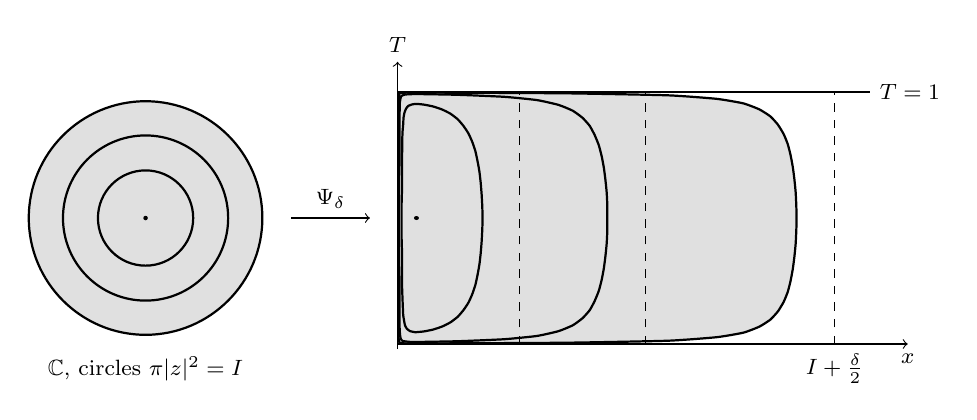
\begin{tikzpicture}[font=\footnotesize]
 \begin{scope}[scale=2.4]
  \fill[black!12] (0,0) circle (0.618);
  \draw[thick] (0,0) circle (0.252);
  \draw[thick] (0,0) circle (0.437);
  \draw[thick] (0,0) circle (0.618);
  \fill (0,0) circle (0.012);
  \node at (0,-0.8) {$\C$, circles $\pi|z|^2=I$};
 \end{scope}
 \draw[->] (1.85,0) -- node[above] {$\Psi_\delta$} (2.85,0);
 \begin{scope}[shift={(3.2,-1.6)},x=4cm,y=3.2cm]
  \fill[black!12] plot[smooth cycle,tension=0.3] coordinates {(0.060,0.002) (0.529,0.005) (0.858,0.013) (1.013,0.027) (1.098,0.045) (1.149,0.069) (1.184,0.097) (1.208,0.130) (1.226,0.167) (1.239,0.207) (1.248,0.251) (1.255,0.298) (1.260,0.346) (1.264,0.397) (1.266,0.448) (1.267,0.500) (1.266,0.552) (1.264,0.603) (1.260,0.654) (1.255,0.702) (1.248,0.749) (1.239,0.793) (1.226,0.833) (1.208,0.870) (1.184,0.903) (1.149,0.931) (1.098,0.955) (1.013,0.973) (0.858,0.987) (0.529,0.995) (0.060,0.998) (0.009,0.996) (0.005,0.989) (0.004,0.977) (0.003,0.960) (0.003,0.937) (0.003,0.910) (0.003,0.879) (0.003,0.843) (0.003,0.803) (0.003,0.760) (0.003,0.714) (0.003,0.666) (0.003,0.616) (0.003,0.565) (0.003,0.513) (0.003,0.461) (0.003,0.409) (0.003,0.359) (0.003,0.310) (0.003,0.262) (0.003,0.218) (0.003,0.177) (0.003,0.139) (0.003,0.105) (0.003,0.076) (0.003,0.051) (0.003,0.031) (0.004,0.016) (0.006,0.006) (0.026,0.002)};
  \draw[thick] plot[smooth cycle,tension=0.3] coordinates {(0.060,0.047) (0.084,0.050) (0.112,0.057) (0.141,0.069) (0.168,0.086) (0.191,0.108) (0.209,0.134) (0.225,0.164) (0.237,0.197) (0.247,0.234) (0.254,0.274) (0.260,0.316) (0.264,0.360) (0.267,0.406) (0.269,0.453) (0.270,0.500) (0.269,0.547) (0.267,0.594) (0.264,0.640) (0.260,0.684) (0.254,0.726) (0.247,0.766) (0.237,0.803) (0.225,0.836) (0.209,0.866) (0.191,0.892) (0.168,0.914) (0.141,0.931) (0.112,0.943) (0.084,0.950) (0.060,0.953) (0.047,0.951) (0.034,0.945) (0.027,0.934) (0.022,0.918) (0.019,0.898) (0.018,0.873) (0.016,0.844) (0.015,0.812) (0.015,0.776) (0.014,0.737) (0.014,0.695) (0.014,0.651) (0.014,0.606) (0.013,0.559) (0.013,0.512) (0.013,0.464) (0.013,0.417) (0.014,0.371) (0.014,0.327) (0.014,0.284) (0.014,0.244) (0.015,0.206) (0.016,0.172) (0.017,0.141) (0.018,0.114) (0.021,0.091) (0.024,0.073) (0.030,0.060) (0.040,0.051) (0.055,0.047)};
  \draw[dashed] (0.388,0) -- (0.388,1);
  \draw[thick] plot[smooth cycle,tension=0.3] coordinates {(0.060,0.008) (0.191,0.011) (0.339,0.019) (0.443,0.032) (0.511,0.051) (0.556,0.074) (0.587,0.102) (0.610,0.134) (0.626,0.171) (0.639,0.211) (0.648,0.254) (0.655,0.300) (0.660,0.348) (0.664,0.398) (0.666,0.449) (0.666,0.500) (0.666,0.551) (0.664,0.602) (0.660,0.652) (0.655,0.700) (0.648,0.746) (0.639,0.789) (0.626,0.829) (0.610,0.866) (0.587,0.898) (0.556,0.926) (0.511,0.949) (0.443,0.968) (0.339,0.981) (0.191,0.989) (0.060,0.992) (0.024,0.990) (0.012,0.984) (0.009,0.972) (0.007,0.955) (0.007,0.932) (0.006,0.905) (0.006,0.874) (0.006,0.839) (0.006,0.799) (0.006,0.757) (0.006,0.712) (0.005,0.664) (0.005,0.615) (0.005,0.564) (0.005,0.513) (0.005,0.461) (0.005,0.410) (0.005,0.360) (0.005,0.312) (0.006,0.265) (0.006,0.221) (0.006,0.181) (0.006,0.143) (0.006,0.110) (0.006,0.081) (0.007,0.056) (0.008,0.036) (0.010,0.022) (0.016,0.012) (0.043,0.008)};
  \draw[dashed] (0.788,0) -- (0.788,1);
  \draw[thick] plot[smooth cycle,tension=0.3] coordinates {(0.060,0.002) (0.529,0.005) (0.858,0.013) (1.013,0.027) (1.098,0.045) (1.149,0.069) (1.184,0.097) (1.208,0.130) (1.226,0.167) (1.239,0.207) (1.248,0.251) (1.255,0.298) (1.260,0.346) (1.264,0.397) (1.266,0.448) (1.267,0.500) (1.266,0.552) (1.264,0.603) (1.260,0.654) (1.255,0.702) (1.248,0.749) (1.239,0.793) (1.226,0.833) (1.208,0.870) (1.184,0.903) (1.149,0.931) (1.098,0.955) (1.013,0.973) (0.858,0.987) (0.529,0.995) (0.060,0.998) (0.009,0.996) (0.005,0.989) (0.004,0.977) (0.003,0.960) (0.003,0.937) (0.003,0.910) (0.003,0.879) (0.003,0.843) (0.003,0.803) (0.003,0.760) (0.003,0.714) (0.003,0.666) (0.003,0.616) (0.003,0.565) (0.003,0.513) (0.003,0.461) (0.003,0.409) (0.003,0.359) (0.003,0.310) (0.003,0.262) (0.003,0.218) (0.003,0.177) (0.003,0.139) (0.003,0.105) (0.003,0.076) (0.003,0.051) (0.003,0.031) (0.004,0.016) (0.006,0.006) (0.026,0.002)};
  \draw[dashed] (1.388,0) -- (1.388,1);
  \draw (0,0) -- (1.5,0);
  \draw (0,1) -- (1.5,1) node[right] {$T=1$};
  \draw[->] (0,-0.02) -- (0,1.12) node[above] {$T$};
  \draw[->] (0,0) -- (1.62,0) node[below] {$x$};
  \fill (0.06,0.5) circle (0.008);
  \node[below] at (1.388,0) {$I+\frac\delta2$};
 \end{scope}
\end{tikzpicture}
\caption{The disc-to-strip map $\Psi_\delta$ of Proposition~\ref{prop:str-strip}: computed level sets for $b_{\rm st}=\delta/\pi=0.12$
and $I=0.2,\,0.6,\,1.2$. The circle of area $I$ goes to the level set $\{R_{\rm st}+V_{\rm st}=\mathcal E_{\rm st}(I)\}$, of
area $I$, inside $\{x<I+\frac\delta2\}$ (dashed); the dot is the common minimum $(b_{\rm st}/2,\frac12)$. Axes not to the same scale.}
\label{fig:str-strip}
\end{figure}

\begin{proof}
(i), (ii) Lemma~\ref{lem:str-normalisation}(iii) applied to $\mathcal J_{\rm st}$ and $F_{\rm st}$ (Lemma~\ref{lem:str-morse-inverse}(iv)), with $\mathfrak a_{\rm st}\to\infty$ by Lemma~\ref{lem:str-area}(iii); the level identity follows from $R_{\rm st}\circ X_{\rm st}+V_{\rm st}\circ Y_{\rm st}=|\xi|^2$.
(iii) Let $I=\pi|z|^2$, $\mathcal E=\mathcal E_{\rm st}(I)$; by Lemma~\ref{lem:str-area}(iii), $I\ge\mathcal E-b_{\rm st}(\frac\pi2-1)$. By (ii) and $V_{\rm st}\ge0$, $R_{\rm st}(x)\le\mathcal E$, so Lemma~\ref{lem:str-area}(i) gives $x<\mathcal E+b_{\rm st}\le I+b_{\rm st}\tfrac\pi2=I+\tfrac\delta2$; the remaining bounds hold since $\Psi_\delta$ maps into the strip.
(iv) Since $\mathcal E_{\rm st}$ increases and $I_{\max}\ge\mathcal E_{\rm st}(I_{\max})-b_{\rm st}(\frac\pi2-1)$ (Lemma~\ref{lem:str-area}(iii)), $\mathcal E=\mathcal E_{\rm st}(\pi|z|^2)\le\mathcal E_{\max}$. By (ii), $R_{\rm st}(x)\le\mathcal E_{\max}$, so $x\ge x_-(\mathcal E_{\max})>0$ (Lemma~\ref{lem:str-area}(i)); and $V_{\rm st}(T)\le\mathcal E_{\max}$, i.e.\ $2\sqrt{T(1-T)}\ge(1+\mathcal E_{\max}/b_{\rm st})^{-1}$, equivalently $(T-\frac12)^2=\frac14-T(1-T)\le\frac14[1-(1+\mathcal E_{\max}/b_{\rm st})^{-2}]$.
\end{proof}

\subsection{Enlarged capacities}\label{sec:str-balls}

The higher-dimensional layer maps of~\cite{SongHD} and the four-dimensional ones of \S\ref{sec:shd-four} use the
following capacities between $\rho_i$ and the auxiliary capacities $a_i$.

\begin{definition}[Enlarged capacities]\label{def:str-enlarged}
\lean{SymplecticPacking.HighDim.RawToricModel.packingSource,
SymplecticPacking.Branch2.CubicData.rhoBar, SymplecticPacking.Branch2.CubicData.deltaStrip,
SymplecticPacking.Branch2.CubicData.rhoHat}
For $1\le i\le k$ put
\[
 \delta_i=\frac{a_i-\rho_i}2,\qquad
 \bar\rho_i=a_i-\frac34\delta_i,\qquad \hat\rho_i=a_i-\frac{\delta_i}2 .
\]
($\bar\rho_i$: closed enlarged source capacity; $\hat\rho_i$: open domain capacity.) Then
$\rho_i<\frac{\rho_i+a_i}2=a_i-\delta_i<\bar\rho_i<\hat\rho_i<a_i$. Put
$\varepsilon_i=(a_i-\hat\rho_i)/4=\delta_i/8$; the $i$-th ball is placed by $\Psi_{\varepsilon_i}$.
In the four-dimensional branch (\S\ref{sec:shd-four}) the same letters denote different values:
there $\bar\rho_i=(\rho_i+a_i)/2=a_i-\delta_i$, $\hat\rho_i=a_i-\frac34\delta_i$, and the $i$-th ball is placed by
$\Psi_{\delta_i}$ (Proposition~\ref{prop:shd4-maps}). The two branches never occur together.
\end{definition}

\section{Return to the four-ball}\label{sec:rtc}

We use the torus cover of \S\ref{sec:fer} and unit representatives in $\C^3\times\C$. Write $\mathcal F(Z)=Z_0^3+Z_1^3+Z_2^3$, fix $0<h<d_n<1/3$, and put $\mathcal N_h=\{(Z,U):|Z|=1,\ \mathcal F(Z)=0,\ \pi|U|^2\le h\}$. The cover map $\mathsf N(u,v,w)=(Z(u,v),w)$ takes $\{p\le h\}$ into $\mathcal N_h$. The three marked base points are the zeros of $Z_0$ on the torus; on the cover, the zero set is their $\Z^2$-periodic inverse image (Lemma~\ref{lem:fer-bpoints}). Pairs are gauge equivalent if $(Z',U')=(cZ,c^3U)$ with $|c|=1$.

\subsection{Conventions and the ambient form}\label{sec:rtc-conventions}

For $Z\ne0$ put $\eta_H=\operatorname{Im}(Z^*dZ)/(2\pi|Z|^2)$ and $\omega_{\rm FS}=d\eta_H=dd^c\log|Z|^2$. For unit $Z$ put $H_Z=\{\xi:Z^*\xi=0\}$. On $H_Z$ one has $\omega_{\rm FS}(\xi_1,\xi_2)=\pi^{-1}\operatorname{Im}(\xi_1^*\xi_2)$, because the terms of $d\eta_H$ containing $d|Z|^2=2\operatorname{Re}(Z^*\,\cdot\,)$ vanish there. All forms below are gauge invariant and annihilate the gauge generator, so they descend to the quotient; we evaluate them on horizontal representatives.

\begin{definition}[Ambient potential on representatives]\label{def:rtc-ambient}
\lean{SymplecticPacking.Return.PhiE,SymplecticPacking.Return.lamE,SymplecticPacking.Return.OmegaE}
On $(\C^3\setminus0)\times\C$ set
\[
 q(Z,W)=\frac{|W|^2}{|Z|^6},\quad
 \Phi_E^{(\delta)}=\log|Z|^2+\delta\log(1+q),\quad
 \Omega_E^{(\delta)}=dd^c\Phi_E^{(\delta)},\quad \Omega_E=\Omega_E^{(d_n)}.
\]
On unit representatives put $p_W=d_n|W|^2/(1+|W|^2)$ and
$X_T=\{(Z,W):|Z|=1,\ \mathcal F(Z)=TW\}$.
Use $E_3$ as shorthand for these representative data with gauge $(Z,W)\sim(cZ,c^3W)$.
For $W\ne0$, write $\alpha=d\arg W/(2\pi)-3\eta_H$.
\end{definition}

A unit phase $e^{i\chi}$ shifts $\eta_H$ by $d\chi/(2\pi)$ and the fibre angular form by $3d\chi/(2\pi)$. Hence $\alpha$ is gauge invariant and vanishes on the gauge generator.

\begin{lemma}[$d^c$ of the norm]\label{lem:rtc-dc}
\lean{SymplecticPacking.Return.dc_log_normW, SymplecticPacking.Return.dc_log_one_add}
\uses{def:rtc-ambient}
On $\{W\ne0\}$, $d^c\log\|W\|^2=\alpha$. On $E_3$,
\[
 d^c\log\big(1+\|W\|^2\big)=\frac{\|W\|^2}{1+\|W\|^2}\,\alpha ,
\]
where the right side extends smoothly across $\{W=0\}$.
\end{lemma}

\begin{proof}
Choose a holomorphic lift $\hat Z$ and a fibre coordinate $\upsilon$ with $[Z,W]=[\hat Z,\upsilon]$. Then $\|W\|^2=|\upsilon|^2\|\hat Z\|^{-6}$ and $\arg W=\arg\upsilon$. Moreover $\eta_H=d^c\log\|\hat Z\|^2$, since $\operatorname{Re}(\hat Z^\dagger d\hat Z)=\frac12d\|\hat Z\|^2$. Hence $d^c\log\|W\|^2=d\arg\upsilon/2\pi-3\,d^c\log\|\hat Z\|^2=\alpha$.

The second identity follows from $d^c\phi(\mu)=\phi'(\mu)\mu\,d^c\log\mu$ with $\mu=\|W\|^2$. Smoothness follows from $\|W\|^2\alpha=\|\hat Z\|^{-6}[(\operatorname{Re}\upsilon\,d\operatorname{Im}\upsilon-\operatorname{Im}\upsilon\,d\operatorname{Re}\upsilon)/2\pi-3|\upsilon|^2d^c\log\|\hat Z\|^2]$.
\end{proof}

\begin{lemma}[The horizontal Hermitian blocks]\label{lem:rtc-kahler}
\lean{SymplecticPacking.Return.OmegaE_closed,SymplecticPacking.Return.OmegaE_herm,SymplecticPacking.Return.OmegaE_pos}
At $|Z|=1$, for $(\xi,\varsigma)\in H_Z\times\C$,
\begin{equation}\label{eq:rtc-OmegaE}
 \Omega_E^{(\delta)}((\xi_1,\varsigma_1),(\xi_2,\varsigma_2))
 =\frac1\pi\operatorname{Im}(A_\delta\xi_1^*\xi_2+B_\delta\bar\varsigma_1\varsigma_2),\quad
 A_\delta=1-\frac{3\delta|W|^2}{1+|W|^2},\quad B_\delta=\frac{\delta}{(1+|W|^2)^2}.
\end{equation}
For $\delta=d_n$, $A>1-3d_n>0$ and $B>0$.
The form is closed, and its restriction to every complex horizontal constraint kernel
$\{(\xi,\varsigma):d\mathcal F_Z\xi=T\varsigma\}$ is nondegenerate.
\end{lemma}

\begin{proof}
Since $q$ is $(\lambda Z,\lambda^3W)$-invariant for $\lambda\in\C^*$, it suffices to work on $H_Z\times\C$ at $|Z|=1$. There $\partial q=\bar W\,dW$, and
$\partial\bar\partial\log(1+q)=\frac{dW\wedge d\bar W}{(1+|W|^2)^2}-\frac{3|W|^2}{1+|W|^2}\sum_jdZ_j\wedge d\bar Z_j$, with no mixed terms. Applying $dd^c=\frac i{2\pi}\partial\bar\partial$ and adding $\omega_{\rm FS}$ gives \eqref{eq:rtc-OmegaE}. For $\delta=d_n$ the Hermitian form $A\xi_1^*\xi_2+B\bar\varsigma_1\varsigma_2$ is positive definite, so its imaginary part is nondegenerate on every complex subspace. Closedness is $d\,dd^c=0$.
\end{proof}

\subsection{The central normal injection}\label{sec:rtc-injection}

\begin{construction}[Weight-three injection]\label{cons:rtc-injection}
\lean{SymplecticPacking.Return.injection}
\uses{def:rtc-ambient, def:cub-model}
For a unit pair $(Z,U)$ with $p<d_n$ put
\[
 \iota[Z,U]=[Z,W],\qquad W=\frac{\sqrt\pi\,U}{\sqrt{d_n-p}},\qquad p=\pi|U|^2 .
\]
\end{construction}

\begin{lemma}[The fibre injection]\label{lem:rtc-injection}
\lean{SymplecticPacking.Return.injection_bijective,SymplecticPacking.Return.injection_normW,SymplecticPacking.Return.injection_pW,SymplecticPacking.Return.injection_normW_le}
At each unit $Z$, the radial maps
\[
 U\mapsto\frac{\sqrt\pi\,U}{\sqrt{d_n-\pi|U|^2}},\qquad
 W\mapsto W\sqrt{\frac{d_n}{\pi(1+|W|^2)}}
\]
are smooth inverses from $\{\pi|U|^2<d_n\}$ to $\C$ and back.
They commute with the weight-three gauge action and preserve $Z$.
Moreover $|W|^2=p/(d_n-p)$, $p_W=p$, and on $\mathcal N_h$ one has $|W|^2\le h/(d_n-h)$.
\end{lemma}

\begin{proof}
Substitute each radial expression into the other and use positivity of its denominator.
The norm and moment identities follow by squaring the positive radial factor.
The last bound follows from the increasing function $p\mapsto p/(d_n-p)$.
\end{proof}

\begin{proposition}[The central pullback on the cover]\label{prop:rtc-central}
\lean{SymplecticPacking.Return.injection_pullback}
On $\{p<d_n\}$ in the torus cover,
$(\iota\circ\mathsf N)^*\Omega_E=\Omega_0$.
\end{proposition}

\begin{proof}
By Lemma~\ref{lem:rtc-dc}, $d^c\Phi_E=\eta_H+p_W\alpha$. Along $\iota$ we have $p_W=p$ and $\arg W=\arg U$ (Lemma~\ref{lem:rtc-injection}). Along $\mathsf N$ we have $Z^*\eta_H=\eta$ and $U=w$. Hence $(\iota\circ\mathsf N)^*d^c\Phi_E=(1-3p)\eta+\frac12\operatorname{Im}(\bar w\,dw)$, which is smooth across $w=0$ and has exterior derivative $\Omega_0$ by Lemma~\ref{lem:fer-Omega0}.
\end{proof}

\subsection{Transport to $T=1$}\label{sec:rtc-transport}

The transport field is the lift of $\partial_T$ that preserves the constraint and is $\Omega_E$-orthogonal to $TX_T=\ker d(\mathcal F(Z)-TW)$.

\begin{construction}[Transport field]\label{cons:rtc-transport}
\lean{SymplecticPacking.Return.nvec, SymplecticPacking.Return.Gfun, SymplecticPacking.Return.Nden,
 SymplecticPacking.Return.transportField}
\uses{lem:rtc-kahler}
For $(Z,W,T)\in S^5\times\C\times\R$ put $f=\mathcal F(Z)$, $\bar Z^2=(\bar Z_0^2,\bar Z_1^2,\bar Z_2^2)$,
\[
 n=3\bar Z^2-3\bar fZ,\qquad G=\|n\|^2,\qquad N_{\rm den}=\frac GA+\frac{T^2}B ,
\]
with $A,B$ as in Lemma~\ref{lem:rtc-kahler}. On the open set $\mathcal O=\{N_{\rm den}>0\}$ define
\begin{equation}\label{eq:rtc-transport}
 \dot Z=\frac{W\,n}{A\,N_{\rm den}},\qquad \dot W=-\frac{T\,W}{B\,N_{\rm den}},\qquad \dot T=1 .
\end{equation}
\end{construction}

Since $A,B>0$, $N_{\rm den}\ge0$ with equality only where $T=0$ and $n=0$; so $\mathcal O$ is the complement of $\{T=0,\ n=0\}$, on which the field is smooth.

\begin{lemma}[Properties of the transport field]\label{lem:rtc-transport-field}
\lean{SymplecticPacking.Return.n_horizontal, SymplecticPacking.Return.n_dF, SymplecticPacking.Return.G_eq,
 SymplecticPacking.Return.transport_gaugeEquiv, SymplecticPacking.Return.transport_horizontal,
 SymplecticPacking.Return.transport_constraint, SymplecticPacking.Return.transport_normW,
 SymplecticPacking.Return.transport_orthogonal, SymplecticPacking.Return.transport_isotropic}
\uses{cons:rtc-transport, lem:rtc-kahler}
\begin{enumerate}[label=(\roman*)]
\item $Z^\dagger n=0$, $n^\dagger\xi=d\mathcal F_Z(\xi)$ for $\xi\in H_Z$, and $G=9\sum_j|Z_j|^4-9|f|^2$.
\item The field is equivariant under $(Z,W)\mapsto(e^{i\chi}Z,e^{3i\chi}W)$ and satisfies $Z^\dagger\dot Z=0$; hence it is
tangent to $S^5\times\C\times\R$. Its horizontal component is $V=(\dot Z,\dot W)\in H_Z\times\C$.
\item Along the field, $\frac{d}{dT}\mathcal F(Z)=\frac{WG}{AN_{\rm den}}=\frac{d}{dT}(TW)$, so $\mathcal F(Z)-TW$ is constant;
$\|Z\|$ is constant; and $\frac{d}{dT}|W|^2=-\frac{2T|W|^2}{BN_{\rm den}}\le0$ for $T\ge0$.
\item At a point of $X_T\times\{T\}$ in $\mathcal O$, $V$ is $\Omega_E$-orthogonal to $\ker(d\mathcal F_Z,-T)\subset H_Z\times\C$.
\end{enumerate}
\end{lemma}

\begin{proof}
(i) Since $Z^\dagger(3\bar Z^2)=3\bar f$, $n$ is the orthogonal projection of $3\bar Z^2$ to $H_Z$. This gives $Z^\dagger n=0$ and $G=\|3\bar Z^2\|^2-|3\bar f|^2$. For $\xi\in H_Z$, $d\mathcal F_Z(\xi)=(3\bar Z^2)^\dagger\xi=n^\dagger\xi$.

(ii) Under the gauge action $f\mapsto e^{3i\chi}f$ and $n\mapsto e^{-2i\chi}n$, while $G,A,B,N_{\rm den}$ are invariant. Tangency follows from (i). Finally, $H_Z\times\C$ is a complement to the kernel $\langle(iZ,3iW)\rangle$ of $T(S^5\times\C)\to TE_3$.

(iii) By (i), $\frac{d}{dT}\mathcal F(Z)=n^\dagger\dot Z$ and $\frac{d}{dT}(TW)=W+T\dot W$. The remaining claims follow from $\frac{d}{dT}\|Z\|^2=2\operatorname{Re}(Z^\dagger\dot Z)$ and $\frac{d}{dT}|W|^2=2\operatorname{Re}(\bar W\dot W)$.

(iv) By (i), $\ker(d\mathcal F_Z,-T)\cap(H_Z\times\C)$ is the kernel of $\ell(\xi,\varsigma)=n^\dagger\xi-T\varsigma$. Let $\mathfrak h=A\,\xi_1^\dagger\xi_2+B\,\bar\varsigma_1\varsigma_2$ and $\nu_\ell=(n/A,-T/B)$. Then $\mathfrak h(\nu_\ell,\kappa)=\ell(\kappa)$. Since $V=(W/N_{\rm den})\nu_\ell$ and $\mathfrak h$ is conjugate linear in its first slot, $\mathfrak h(V,\kappa)=0$ on $\ker\ell$, so $\Omega_E(V,\kappa)=\frac1\pi\operatorname{Im}\mathfrak h(V,\kappa)=0$. Also $\ell(V)=W$. Hence the field is the unique $\Omega_E$-orthogonal lift of $\partial_T$ preserving the constraint.
\end{proof}

\begin{lemma}[Denominator]\label{lem:rtc-denominator}
\lean{SymplecticPacking.Return.Nden_pos, SymplecticPacking.Return.Nden_lower}
\uses{cons:rtc-transport, lem:rtc-transport-field}
Let $\mathcal C=\{(Z,W,T):\|Z\|=1,\ \mathcal F(Z)=TW,\ 0\le T\le1\}$. On $\mathcal C$, $N_{\rm den}>0$: for $T=0$ one has $G\ge3$
and $N_{\rm den}\ge3$, and for $T>0$, $N_{\rm den}\ge T^2/B>0$. If moreover $|W|\le W_{\max}$ and
$T_0=\min\big(1,1/(\sqrt6\max(1,W_{\max}))\big)$, then $N_{\rm den}\ge\min\big(\frac32,\,T_0^2/d_n\big)$.
\end{lemma}

\begin{proof}
By Cauchy--Schwarz $\sum_j|Z_j|^4\ge\frac13$; since $0<A\le1$, $N_{\rm den}\ge G$; and $|f|=T|W|$ on $\mathcal C$. If $T=0$, $G=9\sum_j|Z_j|^4\ge3$. If $T\le T_0$, $9|f|^2\le9T_0^2W_{\max}^2\le\frac32$, so $G\ge\frac32$. If $T\ge T_0$, $N_{\rm den}\ge T^2/B\ge T_0^2/d_n$, since $B\le d_n$.
\end{proof}

\begin{proposition}[Protected transport]\label{prop:rtc-transport}
\lean{SymplecticPacking.Return.transport_mem,SymplecticPacking.Return.transport_hasDerivAt,SymplecticPacking.Return.transport_smooth,SymplecticPacking.Return.transport_injective,SymplecticPacking.Return.transport_pullback}
Fix $w_*=h/(d_n-h)$ and let $\tau_T$ be the flow, from $T=0$, of the cut field defined in the proof. It is a smooth
injective map, commuting with the gauge action. For every unit pair $(Z,W)\in X_0$ with $|W|^2\le w_*$ the trajectory
solves \eqref{eq:rtc-transport} on $[0,1]$, stays in $X_T\cap\{|W|^2\le w_*\}$, and $\tau_1$ maps
$X_0\cap\{|W|^2\le w_*\}$ into $X_1$ with $\tau_1^*(\Omega_E|_{X_1})=\Omega_E|_{X_0}$ there.
\end{proposition}

\begin{proof}
\emph{Cut field.} Let $T_0=T_0(\sqrt{w_*})$ and $c_*=\min(\frac32,T_0^2/d_n)$. For $a<b$ write $S_{a,b}(x)=S((x-a)/(b-a))$ and $P_{a,b,c,d}(x)=S_{a,b}(x)(1-S_{c,d}(x))$, and put
\[
 \chi=S_{c_*/2,3c_*/4}(N_{\rm den})\,P_{1/2,3/4,5/4,3/2}(|Z|^2)\,S_{0,1}(w_*+2-|W|^2)\,P_{-1,-1/2,3/2,2}(T).
\]
Off the unit sphere, $n$ is replaced by $3\bar Z^2-3\bar fZ/|Z|^2$ in computing $N_{\rm den}$. The field $\chi\cdot(\dot Z,\dot W,1)$ is smooth, since its first factor vanishes where $N_{\rm den}\le c_*/2$. It is supported in $\{\frac12\le|Z|^2\le\frac32,\ |W|^2\le w_*+2,\ |T|\le2\}$, so its flow is complete, with diffeomorphic time-$T$ maps. The flow is gauge equivariant because $\chi$ is gauge invariant and the field is equivariant (Lemma~\ref{lem:rtc-transport-field}(ii)).

\emph{Trajectories.} On $\mathcal C_*=\{|Z|=1,\ \mathcal F(Z)=TW,\ |W|^2\le w_*,\ 0\le T\le1\}$ we have $\chi=1$, by Lemma~\ref{lem:rtc-denominator} with $W_{\max}=\sqrt{w_*}$. By Lemma~\ref{lem:rtc-transport-field}(iii), uncut trajectories from $X_0\cap\{|W|^2\le w_*\}$ stay in $\mathcal C_*$, so by uniqueness they coincide with cut trajectories on $[0,1]$.

\emph{Pullback.} Let $F(\sigma,T)=\tau_T(x(\sigma))$ for a smooth family $x(\sigma)$ of initial points. Since $\mathcal F(Z)-TW\equiv0$ along $F$, each tangent vector $(\kappa,t)$ satisfies $\ell(\kappa)=tW$, where $\ell=(d\mathcal F_Z,-T)$. Replacing $\kappa$ by its horizontal representative $\kappa_H$ modulo $G_{\rm gauge}=(iZ,3iW)$ changes neither the constraint, since $\ell(G_{\rm gauge})=3i(\mathcal F(Z)-TW)=0$, nor the pairing with $\Omega_E$. Now $\partial_TF=(V,1)$ with $\ell(V)=W$, so $\kappa_H-tV\in\ker\ell$. Lemma~\ref{lem:rtc-transport-field}(iv) then gives $\Omega_E(V,\kappa)=0$, i.e.\ $\iota_{\partial_T}F^*\Omega_E=0$. Since $F^*\Omega_E$ is closed, Cartan's formula gives $\partial_T(F_T^*\Omega_E)=0$, hence $F_1^*\Omega_E=F_0^*\Omega_E$.
\end{proof}

\subsection{Return to the Fubini--Study form}\label{sec:rtc-return}

On $X_1$ we have $W=\mathcal F(Z)$, so $\mathrm{pr}$ has inverse $\mathrm{gr}[Z]=[Z,\mathcal F(Z)]$. Let $u=|\mathcal F(Z)|^2/\|Z\|^6$, which is smooth on unit representatives. For $s\in\R$ put $\omega^{\rm gr}_s=\omega_{\rm FS}+s\,d_n\,dd^c\log(1+u)=\mathrm{gr}^*\Omega_E^{(sd_n)}$, where the equality uses $\mathrm{gr}^*\|W\|^2=u$. Then $\omega^{\rm gr}_0=\omega_{\rm FS}$ and $\omega^{\rm gr}_1=\mathrm{gr}^*\Omega_E=(\mathrm{pr}^{-1})^*(\Omega_E|_{X_1})$. The return is the Moser flow of this path, which requires $\iota_{Y_s}\omega^{\rm gr}_s=-d_n\,d^c\log(1+u)$; this is solved in closed form because $n$ is an eigenvector of $M_s$.

\begin{construction}[Return field]\label{cons:rtc-return}
\lean{SymplecticPacking.Return.omegaS, SymplecticPacking.Return.returnField}
\uses{lem:rtc-transport-field}
In unit representatives, with $f$, $n$, $G$ as in Construction~\ref{cons:rtc-transport}, put
\[
 A_s=1-3s\,d_n\frac{u}{1+u},\qquad B_s=\frac{s\,d_n}{(1+u)^2},\qquad M_s=A_sI+B_s\,nn^\dagger\ \text{ on }H_Z,
\]
\begin{equation}\label{eq:rtc-return-field}
 Y_s=-\frac{d_n}{2}\,\frac{f\,n}{(1+u)(A_s+B_sG)}\in H_Z .
\end{equation}
\end{construction}

\begin{lemma}[Graph forms]\label{lem:rtc-graph}
\lean{SymplecticPacking.Return.omegaS_graph, SymplecticPacking.Return.OmegaE_herm,
 SymplecticPacking.Return.As_gt_half, SymplecticPacking.Return.Bs_nonneg, SymplecticPacking.Return.returnDen_gt_half, SymplecticPacking.Return.Ms_nvec}
\uses{cons:rtc-return, lem:rtc-kahler}
For $s\in[0,1]$ and $\xi_1,\xi_2\in H_Z$, $\omega^{\rm gr}_s(\xi_1,\xi_2)=\frac1\pi\operatorname{Im}(\xi_1^\dagger M_s\xi_2)$. Moreover
$u\le1$, $A_s\ge1-\frac32d_n>\frac12$ and $B_s\ge0$; hence $M_s\ge\frac12I$ and every $\omega^{\rm gr}_s$ is positive on $H_Z$.
\end{lemma}

\begin{proof}
By Lemma~\ref{lem:rtc-transport-field}(i), $d\,\mathrm{gr}(\xi)$ is represented by $(\xi,n^\dagger\xi)$ in the gauge of Lemma~\ref{lem:rtc-kahler}. Since $|W|^2=u$ at $W=\mathcal F(Z)$, \eqref{eq:rtc-OmegaE} gives the Hermitian form $A_s\xi_1^\dagger\xi_2+B_s\overline{n^\dagger\xi_1}\,n^\dagger\xi_2=\xi_1^\dagger M_s\xi_2$. For $\|Z\|=1$, $|f|\le\max_j|Z_j|\sum_j|Z_j|^2\le1$. Hence $u\le1$, so $u/(1+u)\le\frac12$ and $A_s\ge1-\frac32d_n>\frac12$, because $d_n<\frac13$.
\end{proof}

\begin{lemma}[$d^c$ along the graph]\label{lem:rtc-dc-horizontal}
\lean{SymplecticPacking.Return.dc_log_one_add_u}
\uses{cons:rtc-return, lem:rtc-transport-field}
For $\xi\in H_Z$ (unit representative), $d^c\log(1+u)(\xi)=\dfrac{\operatorname{Im}\big(\bar f\,n^\dagger\xi\big)}{2\pi(1+u)}$.
\end{lemma}

\begin{proof}
Where $f\ne0$, as in Lemma~\ref{lem:rtc-dc}, $d^c\log(1+u)=\tfrac{u}{1+u}\big(\tfrac{d\arg\mathcal F}{2\pi}-3\eta_H\big)$. On $H_Z$ we have $\eta_H(\xi)=0$ and $d\arg\mathcal F(\xi)=\operatorname{Im}(n^\dagger\xi/f)$, and $u/f=\bar f$. Both sides are smooth, so the identity extends to $\{f=0\}$.
\end{proof}

\begin{lemma}[The return field]\label{lem:rtc-return-field}
\lean{SymplecticPacking.Return.returnField_spec, SymplecticPacking.Return.returnField_gauge}
\uses{lem:rtc-graph, lem:rtc-dc-horizontal}
$Y_s$ is smooth in $(s,Z)$ for $s$ in a neighbourhood of $[0,1]$, gauge equivariant and tangent to $S^5$, hence descends to a
time-dependent smooth vector field on unit representatives, and
\[
 \iota_{Y_s}\omega^{\rm gr}_s=-d_n\,d^c\log(1+u)\qquad(s\in[0,1]).
\]
\end{lemma}

\begin{proof}
Under the gauge action $f\mapsto e^{3i\chi}f$ and $n\mapsto e^{-2i\chi}n$, so $Y_s\mapsto e^{i\chi}Y_s$; also $Z^\dagger Y_s=0$. The denominator is positive for $-\frac1{9d_n}<s<\frac2{3d_n}$, an interval containing $[0,1]$: for $s\ge0$, $A_s+B_sG\ge A_s\ge1-\frac32s\,d_n$; for $s<0$, $A_s\ge1$ and $B_sG\ge-9|s|d_n$, because $0\le G\le9$. Since $M_sn=(A_s+B_sG)n$, we get $M_sY_s=-\frac{d_n}2\frac{fn}{1+u}$. Lemmas~\ref{lem:rtc-graph} and~\ref{lem:rtc-dc-horizontal} then give, for $\xi\in H_Z$, $\omega^{\rm gr}_s(Y_s,\xi)=\frac1\pi\operatorname{Im}((M_sY_s)^\dagger\xi)=-d_n\,d^c\log(1+u)(\xi)$.
\end{proof}

\begin{proposition}[Unit-representative return]\label{prop:rtc-return}
\lean[needed]{SymplecticPacking.Return.returnFlow_pullback,SymplecticPacking.Return.returnFlowInv_pullback,
SymplecticPacking.Return.returnFlow_smooth,SymplecticPacking.Return.returnFlowInv_smooth,
SymplecticPacking.Return.returnFlowInv_returnFlow,SymplecticPacking.Return.returnFlow_returnFlowInv,
SymplecticPacking.Return.nsq_returnFlow,SymplecticPacking.Return.returnFlow_gaugeEquiv}
Let $\psi_s$ be the flow from $s=0$ of the cut field of the proof. It is defined for all $s$, preserves $|Z|=1$, commutes
with the gauge action, and its time-$s$ maps are diffeomorphisms. On the unit sphere it is the flow of $Y_s$ for
$s\in[0,1]$, and $\psi_s^*\omega_s^{\rm gr}=\omega_{\rm FS}$. Consequently $(\psi_1^{-1})^*\omega_{\rm FS}=\omega^{\rm gr}_1$, and
$(\psi_1^{-1}\circ\mathrm{pr})^*\omega_{\rm FS}=\Omega_E|_{X_1}$.
\end{proposition}

\begin{proof}
Put $m=1-\frac32d_n>0$ and $D_s=A_s+B_sG$, with $n$ extended off the sphere as in Proposition~\ref{prop:rtc-transport}. The cut field is
\[
 S_{m/2,3m/4}(D_s)\,P_{1/2,3/4,5/4,3/2}(|Z|^2)\,P_{-1,-1/2,3/2,2}(s)\,Y_s .
\]
It is smooth, since the first factor vanishes where $D_s\le m/2$, and compactly supported, so its flow is complete with diffeomorphic time maps. The flow is gauge equivariant by Lemma~\ref{lem:rtc-return-field}, and it preserves the sphere because $2\operatorname{Re}(Z^\dagger Y_s)=0$. For $|Z|=1$ and $s\in[0,1]$, Lemma~\ref{lem:rtc-graph} gives $D_s\ge m$, so the cut field equals $Y_s$ there. Since $\partial_s\omega^{\rm gr}_s=d(d_n\,d^c\log(1+u))$, Cartan's formula and Lemma~\ref{lem:rtc-return-field} give $\frac d{ds}\psi_s^*\omega^{\rm gr}_s=0$. Finally, $\mathrm{gr}\circ\mathrm{pr}=\mathrm{id}$ on $X_1$ gives $\mathrm{pr}^*\omega^{\rm gr}_1=\Omega_E|_{X_1}$.
\end{proof}

\subsection{Equivariant injectivity and the ball chart}\label{sec:rtc-avoid}

From now on, $\mathcal T_{\rm u}$ uses the protected cutoff $w_*=h/(d_n-h)$ and is considered on $\mathcal N_h$. Let $\mathsf r Z=(\zeta Z_0,Z_1,Z_2)$ and $\mathsf r(Z,W)=(\mathsf r Z,W)$; $\mathsf r$ preserves the norm, the Fermat equation and the source moment, and commutes with the unit gauge action.

\begin{lemma}[Fixed representatives modulo gauge]\label{lem:rtc-fixed}
\lean{SymplecticPacking.Return.fixed_CP2,SymplecticPacking.Return.fixed_N}
For a nonzero vector, $\mathsf r Z$ is a scalar multiple of $Z$ exactly when $Z_0=0$ or $Z_1=Z_2=0$.
For a central unit pair $(Z,U)$, the equation $\mathsf r(Z,U)=(cZ,c^3U)$ is possible exactly when $Z_0=0$.
\end{lemma}

\begin{proof}
A nonzero last coordinate forces $c=1$ and then $Z_0=0$. Otherwise both last coordinates vanish, which $\mathcal F(Z)=0$ excludes at a central unit vector. If $Z_0=0$, the pair is fixed with $c=1$.
\end{proof}

\begin{lemma}[Equivariance]\label{lem:rtc-equivariant}
\lean{SymplecticPacking.Return.injection_equivariant, SymplecticPacking.Return.transport_equivariant,
 SymplecticPacking.Return.returnFlow_equivariant, SymplecticPacking.Return.compositeT_equivariant}
\uses{cons:rtc-injection, prop:rtc-transport, prop:rtc-return}
$\mathsf r$ preserves $\mathcal F$, $\omega_{\rm FS}$, $\|W\|$, $\Omega_E$, $u$, each $X_T$ and $\{(Z,U):|Z|=1,\mathcal F(Z)=0,p<d_n\}$, and it maps the fields
\eqref{eq:rtc-transport} and \eqref{eq:rtc-return-field} to themselves. Consequently $\iota$, $\tau_1$, $\mathrm{pr}$, $\psi_1^{-1}$ and
$\mathcal T_{\rm u}$ commute with $\mathsf r$.
\end{lemma}

\begin{proof}
$\mathsf r$ is unitary and $\mathcal F\circ\mathsf r=\mathcal F$, so it preserves all the listed quantities and also $p,A,B,A_s,B_s$. Since $\bar\zeta^2=\zeta$, we have $n(\mathsf rZ)=\mathsf r\,n(Z)$. Hence $G$ and $N_{\rm den}$ are invariant, both fields are $\mathsf r$-equivariant, and by uniqueness so are their flows. $\iota$ commutes with $\mathsf r$ because $p$ is invariant, and $\mathrm{pr}$ does because the lift of $\mathsf r$ to $E_3$ covers $\mathsf r$.
\end{proof}

\begin{lemma}[Injectivity modulo gauge]\label{lem:rtc-injective}
\lean{SymplecticPacking.Return.compositeT_inj_mod_gauge}
For $x,x'\in\mathcal N_h$ and $|c|=1$, the equality
$\mathcal T_{\rm u}(x)=c\mathcal T_{\rm u}(x')$ implies
$x=(cZ',c^3U')$.
\end{lemma}

\begin{proof}
Each factor of $\mathcal T_{\rm u}=\psi_1^{-1}\circ\mathrm{pr}\circ\tau_1\circ\iota$ is injective on representatives: $\iota$ by the explicit inverse of Lemma~\ref{lem:rtc-injection}, $\tau_1$ and $\psi_1^{-1}$ as time maps of complete flows, and $\mathrm{pr}$ on $X_1$, where $W=\mathcal F(Z)$. Each factor also commutes with $(Z,W)\mapsto(cZ,c^3W)$. Hence $c\,\mathcal T_{\rm u}(x')=\mathcal T_{\rm u}(cZ',c^3U')$, and injectivity concludes.
\end{proof}

\begin{proposition}[Avoidance and compact margin]\label{prop:rtc-avoid}
\lean{SymplecticPacking.Return.avoid_L,SymplecticPacking.Return.avoid_L_compact}
If $x=(Z,U)\in\mathcal N_h$ and $Z_0\ne0$, then
$(\mathcal T_{\rm u}(x))_0\ne0$ and its last two coordinates do not vanish together.
On every nonempty compact family of these inputs,
$m_{\mathcal K}=\min_{x\in\mathcal K}|(\mathcal T_{\rm u}(x))_0|^2>0$. For $\mathcal K=\varnothing$ set $m_{\mathcal K}=1$.
\end{proposition}

\begin{proof}
Let $Y=\mathcal T_{\rm u}(x)$. If $Y_0=0$, then $\mathsf rY=Y$, and Lemmas~\ref{lem:rtc-equivariant} and~\ref{lem:rtc-injective} (with $c=1$) give $\mathsf rx=x$. If $Y_1=Y_2=0$, then $\mathsf rY=\zeta Y$, and the same lemmas give $\mathsf rx=(\zeta Z,\zeta^3U)$. In both cases Lemma~\ref{lem:rtc-fixed} gives $Z_0=0$, a contradiction. The compact margin holds because $x\mapsto|(\mathcal T_{\rm u}(x))_0|^2$ is continuous and positive on $\mathcal K$.
\end{proof}

\begin{lemma}[The ball chart on representatives]\label{lem:rtc-ball-chart}
\lean[needed]{SymplecticPacking.Return.ballChart, SymplecticPacking.Return.ballChart_gauge,
 SymplecticPacking.Return.ballChart_symplectic_rep, SymplecticPacking.Return.ballChart_affine,
 SymplecticPacking.Return.ballChart_norm, SymplecticPacking.Return.ballAffine_eq, SymplecticPacking.Return.ballChart_norm_lt}
On $S^5_*=\{Z\in\C^3:|Z|=1,\ Z_0\ne0\}$ put $b_{\rm ball}(Z)=\frac{\bar Z_0}{|Z_0|}\frac{(Z_1,Z_2)}{\sqrt\pi}$. This map is gauge
invariant, $\pi|b_{\rm ball}(Z)|^2=1-|Z_0|^2<1$, and in the affine coordinates $z=(Z_1/Z_0,Z_2/Z_0)$ it is the chart
$\mathrm{ch}(z)=z/\sqrt{\pi(1+|z|^2)}$ of Lemma~\ref{lem:pre-fs}(b). Moreover
$b_{\rm ball}^*\omega_0=\frac1\pi\sum_{j=0}^2dx_j\wedge dy_j\big|_{S^5_*}=\omega_{\rm FS}|_{S^5_*}$, where $Z_j=x_j+iy_j$. Hence
$(b_{\rm ball}\circ\varphi)^*\omega_0=\varphi^*\omega_{\rm FS}$ for every smooth map $\varphi$ of a manifold into $S^5_*$.
\end{lemma}

\begin{proof}
The unit phases cancel, and substituting $Z=e^{i\chi}(1,z)/\sqrt{1+|z|^2}$ gives the affine formula and the norm identity.
Write $e=\bar Z_0/|Z_0|=e^{i\phi}$, $\phi=-\arg Z_0$, and $y_j=eZ_j/\sqrt\pi$ ($j=1,2$). Then
$\bar y_jdy_j=\frac1\pi\big(|Z_j|^2\,\bar e\,de+\bar Z_jdZ_j\big)$ with $\bar e\,de=i\,d\phi$, so the Liouville form
$\lambda_0=\frac12\sum_{j=1}^2\operatorname{Im}(\bar y_jdy_j)$ pulls back to
$\frac1{2\pi}\big((1-|Z_0|^2)d\phi+\sum_{j=1}^2\operatorname{Im}(\bar Z_jdZ_j)\big)$ on $S^5_*$. Since
$\operatorname{Im}(\bar Z_0dZ_0)=|Z_0|^2d\arg Z_0=-|Z_0|^2d\phi$, this equals $\frac1{2\pi}\big(d\phi+\operatorname{Im}(Z^\dagger dZ)\big)$, whose
differential is $\frac1{2\pi}\sum_{j=0}^2d(x_jdy_j-y_jdx_j)=\frac1\pi\sum_jdx_j\wedge dy_j$. As $d\lambda_0=\omega_0$, this proves the first
identity; the second holds because $\frac1{2\pi}\operatorname{Im}(Z^\dagger dZ)=\eta_H$ on the sphere and $d\eta_H=\omega_{\rm FS}$.
\end{proof}

For $y\in\Bo(1)$, $(\sqrt{1-\pi|y|^2},\sqrt\pi\,y_1,\sqrt\pi\,y_2)$ is the unique gauge representative with positive first coordinate of every unit vector with nonzero first coordinate and ball-chart image $y$.

\subsection{The transfer theorem}\label{sec:rtc-transfer}

\begin{theorem}[Transfer on the cover]\label{thm:rtc-transfer}\label{thm:cub-transfer}
\lean[needed]{SymplecticPacking.Return.compositeT_inj_mod_gauge,SymplecticPacking.Return.compositeT_pullback,SymplecticPacking.Return.compositeT_equivariant,SymplecticPacking.Return.avoid_L_compact,
SymplecticPacking.Return.injection_pullback, SymplecticPacking.Return.ballChart_symplectic_rep,
SymplecticPacking.Embed.Cubic.fcap_eq_imp, SymplecticPacking.Embed.Cubic.fcap_eq_imp}
\uses{cons:cub-transfer, prop:rtc-central, prop:rtc-transport, prop:rtc-return, prop:rtc-avoid, lem:rtc-ball-chart}
Let $w_*=h/(d_n-h)$ and $\mathcal T_{\rm u}=\psi_1^{-1}\circ\mathrm{pr}\circ\tau_1\circ\iota$ on $\mathcal N_h$. The cover map
\[
 \mathcal T=b_{\rm ball}\circ\mathcal T_{\rm u}\circ\mathsf N
 \quad\text{on}\quad\{p<h,\ (u,v)\notin\mathcal Z\}
\]
is smooth, invariant under the deck maps, takes values in $\Bo(1)$ and satisfies $\mathcal T^*\omega_0=\Omega_0$. Two points
have the same image if and only if they are deck equivalent. For every compact $\mathcal K$ in the domain,
$\mathcal T(\mathcal K)\subset B(1-m_{\mathcal K})$ with $m_{\mathcal K}>0$ as in Proposition~\ref{prop:rtc-avoid}. In particular the
restriction of $\mathcal T$ to an open set on which it is injective is a symplectic embedding, and $\mathcal T$ carries
pairwise disjoint subsets of its domain, no two points of whose union are deck equivalent, to pairwise disjoint sets.
\end{theorem}

\begin{proof}
On $\{p<h\}$, $\mathsf N$ takes values in $\mathcal N_h$ with $p<d_n$, and $\tau_1\circ\iota$ lands in $X_1\cap\{|W|^2\le w_*\}$ (Lemma~\ref{lem:rtc-injection}, Proposition~\ref{prop:rtc-transport}). Propositions~\ref{prop:rtc-central}, \ref{prop:rtc-transport} and~\ref{prop:rtc-return} give $(\mathcal T_{\rm u}\circ\mathsf N)^*\omega_{\rm FS}=\Omega_0$. For $(u,v)\notin\mathcal Z$, $\mathcal T_{\rm u}(\mathsf N(x))\in S^5_*$ (Proposition~\ref{prop:rtc-avoid}), so Lemma~\ref{lem:rtc-ball-chart} gives $\mathcal T^*\omega_0=\Omega_0$ and $\pi|\mathcal T|^2=1-|(\mathcal T_{\rm u}\mathsf N)_0|^2<1$, whence the margin $m_{\mathcal K}$ on $\mathcal K$. Deck maps change $\mathsf N(x)$ to a gauge-equivalent pair (Construction~\ref{cons:fer-atlas}(b)), $\mathcal T_{\rm u}$ is gauge equivariant and $b_{\rm ball}$ gauge invariant, so $\mathcal T$ is deck invariant. Conversely, if $\mathcal T(x)=\mathcal T(x')$, the ball chart determines a unit vector with nonzero first coordinate up to gauge, so Lemma~\ref{lem:rtc-injective} gives $\mathsf N(x)\sim\mathsf N(x')$; hence $[Z(u,v)]=[Z(u',v')]$ in $\CP^2$, and Lemma~\ref{lem:fer-torus} gives $(u,v)-(u',v')\in\Z^2$. For the corresponding deck map $T$, the unit vectors $Z(u,v)$ agree, so the gauge factor is one and $x=Tx'$. Injective restrictions are injective symplectic immersions in equal dimension, hence open symplectic embeddings; the last assertion follows from the characterisation of equal images.
\end{proof}

All objects are explicit; $\psi_1^{-1}$ is obtained by integrating \eqref{eq:rtc-return-field} backwards from $s=1$, and the transport by \eqref{eq:rtc-transport}.

\subsection{The packing in dimension four}\label{sec:rtc-packing}

The transfer depends on the data only through $h$.

\begin{construction}[Data of the four-dimensional packing]\label{cons:rtc-data}
\uses{M-prop:cmp-linear, def:shd4-data, prop:cub-handle, prop:fer-handle, thm:rtc-transfer, prop:rtc-avoid}
Let $(k,\rho_i,a_i,h,d_n,g,K,q)$ be valid cubic data (Definition~\ref{def:shd4-data}) with $d_n=\frac12(h+\frac13)$. Let
$f_i=f_i^{\rm cap}$ be the maps of Remark~\ref{rem:shd-four}, built by the handle construction of \S\ref{sec:shd-four},
put $\bar\rho_i=(\rho_i+a_i)/2$ and $\hat\rho_i=\bar\rho_i+(a_i-\bar\rho_i)/4$, and let the open domain be
$\Bo(\hat\rho_i)$. Let $\rho_i^+<\rho_i^{\rm dom}$ be the recorded capacities of Remark~\ref{rem:rtc-recorded}. Put
$\mathcal K=\bigcup_i f_i(B(\rho_i^+))$ and $m=\frac12\min_{z\in\mathcal K}(1-\pi|z|^2)$.

\emph{The equal case.} Let $k\ge10$, $\rho_1=\dots=\rho_k=\rho$ and $\frac34<\rho\sqrt k<1$. Put
$t_0=\frac12(1+\rho\sqrt k)$, $a_i=a=t_0/\sqrt k$, $h=t_0/3$, $g=3(1-t_0)$, and let $(K,q)$ be the comparison datum of
\Mref{Proposition}{prop:cmp-linear}, with gap $\frac{31}{32}g$. These are valid cubic data
(Remark~\ref{rem:rtc-equal}). For $k=9$ the same formulas would give $a=t_0/3=h$, violating $a<h$; valid cubic data for
$k=9$ and for unequal capacities are constructed in the companion paper~\cite{SongHD} from a scalar comparison datum.
\end{construction}

\begin{theorem}[Packing in dimension four]\label{thm:cub-packing}\label{prop:rtc-embeddings}
\lean[needed]{SymplecticPacking.Branch2.CubicData.Valid.fcapGen_injective, SymplecticPacking.Embed.Cubic.fcapV_disjoint,
SymplecticPacking.Embed.Cubic.fcapV_mem_ball, SymplecticPacking.Embed.Cubic.fcap_injective, SymplecticPacking.Embed.Cubic.fcap_disjoint,
SymplecticPacking.Embed.Cubic.fcap_mem_ball, SymplecticPacking.Embed.Cubic.handle_phiInvSpec,
SymplecticPacking.Handle.Cubic.handle_deckEquivariant}
\uses{cons:rtc-data, M-prop:cmp-linear, def:shd4-data, prop:cub-handle, prop:fer-handle, thm:rtc-transfer, prop:rtc-avoid}
Let $(k,\rho_i,a_i,h,d_n,g,K,q)$ be valid cubic data with $d_n=\frac12(h+\frac13)$. Then there are explicit numbers
$\rho_i<\rho_i^+<\rho_i^{\rm dom}$ and smooth maps $f_i\colon\Bo(\rho_i^{\rm dom})\to\C^2$ with symplectic derivative, injective
on $B(\rho_i^+)$, such that the sets $f_i(B(\rho_i^+))$ are pairwise disjoint and contained in $B(1-\mu_{\rm ball})$ for some
$\mu_{\rm ball}\in(0,1)$. More precisely, for the data of Construction~\ref{cons:rtc-data}:
\begin{enumerate}[label=(\roman*)]
\item each $f_i$ is a smooth symplectic embedding of $\Bo(\hat\rho_i)$ into $(\Bo(1),\omega_0)$, and
$\rho_i<\rho_i^+<\rho_i^{\rm dom}\le\hat\rho_i$;
\item the sets $f_i(\Bo(\hat\rho_i))$, $1\le i\le k$, are pairwise disjoint;
\item $m>0$ and $f_i(B(\rho_i^+))\subset B(1-m)$ for every $i$;
\item the comparison isotopy $q$, the Moser map $\Phi$, the handle map $\mathcal D$ and the transfer $\mathcal T$ are the same for all $i$;
only the layer map $E_i$ depends on $i$.
\end{enumerate}
\end{theorem}

\begin{proof}
The data are valid cubic data by hypothesis (in the equal case by \Mref{Proposition}{prop:cmp-linear} and Remark~\ref{rem:rtc-equal}), and $h<d_n<\frac13$. Here $f_i=\mathcal T\circ f^N_i$ with $f^N_i$ of Proposition~\ref{prop:shd4-maps} (Remark~\ref{rem:shd-four}).

(i) By Proposition~\ref{prop:shd4-maps}(a), $f^N_i$ is smooth on $\Bo(\hat\rho_i)$ into $\{p<h\}\setminus\widetilde{\mathcal F}$, the domain of $\mathcal T$, with $(f^N_i)^*\Omega_0=\omega_0$; Theorem~\ref{thm:rtc-transfer} gives $f_i$ smooth into $\Bo(1)$ with $f_i^*\omega_0=\omega_0$. If $f_i(X)=f_i(X')$, Theorem~\ref{thm:rtc-transfer} gives $f^N_i(X)=Tf^N_i(X')$ for a deck map $T$, and Proposition~\ref{prop:shd4-maps}(c) gives $X=X'$; so $f_i$ is an open embedding. The capacity inequalities are in Remark~\ref{rem:rtc-recorded}.
(ii) If $f_i(X)=f_j(X')$, the same argument gives $i=j$, $X=X'$.
(iii) $\mathcal K$ is compact in $\Bo(1)$, so $1-\pi|z|^2\ge2m>m>0$ on $\mathcal K$.
(iv) $q$, $\mathcal D$, $\Phi$, $\chi_{\mathcal A}$ and $\mathcal T$ do not depend on $i$.

The first statement follows with $\mu_{\rm ball}=m<1$, restricting $f_i$ to $\Bo(\rho_i^{\rm dom})$.
\end{proof}

\begin{remark}[Recorded capacities]\label{rem:rtc-recorded}
Since the proof embeds the open balls $\Bo(\hat\rho_i)$ with pairwise disjoint images, Theorem~\ref{thm:cub-packing}
holds for every choice of $\rho_i<\rho_i^+<\rho_i^{\rm dom}\le\hat\rho_i$. The choice enters only the radii of the common
isotopy (\Mref{Definition}{def:ham-radii}) and hence the Hamiltonian. In the equal case the construction records
$(\rho_i^+,\rho_i^{\rm dom})=(\rho \varrho_3^2,\rho \varrho_4^2)$, where $\varrho_4=\sqrt{\bar\rho/\rho}$ and $\varrho_3=(1+\varrho_4)/2$; then
$1<\varrho_3<\varrho_4$ gives $\rho<\rho \varrho_3^2<\rho \varrho_4^2=\bar\rho<\hat\rho$. For target capacity $C$ and given capacity $c=C\rho$
the physical map $u\mapsto\sqrt C\,f_i(u/\sqrt C)$ has the capacities $C\rho_i^+$ and $C\rho_i^{\rm dom}$, that is,
$c\varrho_3^2$ and $c\varrho_4^2$. For the valid cubic data of the companion paper~\cite{SongHD} the construction records
$(\rho_i^+,\rho_i^{\rm dom})=(\bar\rho_i,\hat\rho_i)$.
\end{remark}

\begin{remark}[The equal-capacity branch]\label{rem:rtc-equal}\label{rem:cub-lean}
\lean{SymplecticPacking.Params.t0, SymplecticPacking.Params.a, SymplecticPacking.Params.h,
 SymplecticPacking.Params.dn_sub_h, SymplecticPacking.Params.one_sub_three_dn, SymplecticPacking.Params.a_sub_rho,
 SymplecticPacking.Params.density, SymplecticPacking.Branch2.CubicData.ofParams_valid,
 SymplecticPacking.Branch2.embeddingsEq, SymplecticPacking.Branch2.embeddingsEq_spec,
 SymplecticPacking.Branch2.cubicEmbeddings_spec}
\uses{cons:rtc-data, thm:cub-packing, rem:fer-lean}
In the equal case of Construction~\ref{cons:rtc-data} let $\eta_\star=1-\rho\sqrt k\in(0,\frac14)$ be the volume defect. Then
\[
 t_0=1-\frac{\eta_\star}2,\quad a=\frac{t_0}{\sqrt k},\quad h=\frac{t_0}3,\quad d_n=\frac13-\frac{\eta_\star}{12},\qquad
 a-\rho=\frac{\eta_\star}{2\sqrt k},\quad d_n-h=\frac{\eta_\star}{12},\quad 1-3d_n=\frac{\eta_\star}4,
\]
the comparison function is $K(p)=(3\sqrt k-9)p$, and the comparison gap of \Mref{Proposition}{prop:cmp-linear} is
$\frac{31}{32}g$ with $g=3(1-t_0)=\frac{3\eta_\star}2$. With the isotopy of Theorem~\ref{thm:pll-inner} and the handle
construction of \S\ref{sec:shd-four}, the maps of this branch are
\[
 f_i= b_{\rm ball}\circ\psi_1^{-1}\circ\operatorname{pr}\circ\tau_1\circ\iota
       \circ\mathsf N\circ\Phi^{-1}\circ\chi_{\mathcal A}\circ\mathcal D^{-1}\circ E_i\qquad(1\le i\le k).
\]
For the input of \Mref{Corollary}{thm:main-epoch}, $\rho=\sqrt{(1-\eps/2)/k}$ and
$\eta_\star=1-\sqrt{1-\eps/2}\in(\eps/4,\eps/2)$; the equal case applies exactly when $\rho\sqrt k>3/4$, i.e.\ $\eps<\frac78$.
For unit balls (capacity $\pi$) the target capacity is $C=\pi/\rho$, and the
physical rescaling of \Mref{Definition}{def:ham-normalise} makes the target the open Euclidean ball of radius
$R=\rho^{-1/2}$, so $k/R^4=k\rho^2=(1-\eta_\star)^2$. For the data of \Mref{Theorem}{thm:intro-4d}, $R^4=k/(1-\eps/4)$, so
$\rho\sqrt k=\sqrt{1-\eps/4}>\frac34$ and $\eta_\star=1-\sqrt{1-\eps/4}\in(\eps/8,\eps/4)$; the equal case applies
for every $\eps\in(0,1)$ when $k\ge10$. The strip constants are those of Remark~\ref{rem:shd-four} with
$\delta=(a-\rho)/2$.

The defect $1-\rho\sqrt k=\eta_\star$ splits as $(1-t_0)+\sqrt k\,(a-\rho)=\frac{\eta_\star}2+\frac{\eta_\star}2$. The fibre part $1-t_0=1-3h$ pays for
$h<\frac13$, for the comparison gap $g$ and for the margins $d_n-h$ and $1-3d_n$ of the transfer; the strip part $\sqrt k\,(a-\rho)$ pays for the enlargement from $\rho$ to $\bar\rho$ and for the excess of the strip map.
The transfer, the ball chart and the dilation are symplectic embeddings and lose no volume beyond these margins.
\end{remark}


\section{The normalised embeddings of the linear branch}\label{sec:brd}

This section fixes the normalised embeddings used in \Msec{sec:ham-embeddings}.

\begin{construction}[The normalised embeddings]\label{cons:ham-branch}
\uses{thm:cub-packing, cons:rtc-data, rem:rtc-equal, rem:rtc-recorded}
Let $k\ge10$ and $\rho>0$ with $\frac34<\rho\sqrt k<1$, and put $\rho_1=\dots=\rho_k=\rho$ (the \emph{linear branch}).
The \emph{normalised embeddings} $f^\natural_i$ are the maps of Theorem~\ref{thm:cub-packing} for the valid cubic data of
the equal case of Construction~\ref{cons:rtc-data} (Remark~\ref{rem:rtc-equal}); the enlarged capacity and the domain
capacity are $(\rho_i^+,\rho_i^{\rm dom})=(\rho \varrho_3^2,\rho \varrho_4^2)$, as in Remark~\ref{rem:rtc-recorded}.
\end{construction}

The data satisfy $3\rho<1$ and $k\rho^2<1$, so $(2,k,1,\rho)$ is admissible.

\section{The common isotopy and the pushforward of the source primitive}\label{sec:iso}

For $k$ disjoint balls in $\R^{2n}$ we construct one smooth family $F_{i,t}$ of symplectic embeddings from the translations $s_i+u$ to the $f_i$, with disjoint images at all times (Proposition~\ref{prop:iso-common}). The balls are translated to far centres along a route on which they never meet, deformed linearly to $A_i=Df_i(0)$, then to $u\mapsto\tau^{-1}f_i(\tau u)$, and finally dilated by a common parameter running from $\tau$ to $1$. Disjointness comes from separation in the first three stages and from the common dilation in the tail. All ingredients are explicit functions of the input: the maxima defining $L$, the minimum defining $\delta_c$, the positive square root and least admissible angle in the linear path, and the ranks in the route. The pushforward of a cut-off source primitive along $F$ is smooth with compact support (Lemma~\ref{lem:iso-pushforward}), with closed forms on each stage (Lemma~\ref{lem:iso-stage-primitives}).

\emph{Conventions} (\S\ref{sec:pre-conventions}). We write $\omega_0(\xi,\xi')=\langle\xi,J_0\xi'\rangle$ with $J_0=\bigl(\begin{smallmatrix}0&I\\-I&0\end{smallmatrix}\bigr)$ in $(x,y)$, and $\operatorname{Sp}(2n)=\{A:A^{\mathsf T}J_0A=J_0\}$. The matrix $J_\C=-J_0$ is multiplication by $i$ on $\C^n$. Matrices are written in $n\times n$ blocks with respect to $(x,y)$, and linear maps are identified with their matrices. Vector norms are Euclidean and $\|\cdot\|$ is the operator norm. $\EB(y,r)$ and $\EB^\circ(y,r)$ denote the closed and open Euclidean balls, and $\EB(r)=\EB(0,r)$. $S$ is the flat step of Definition~\ref{def:pre-flat}. A matrix-valued function of $\sigma\in\R$ has \emph{smooth entries} if every entry is $C^\infty$ in $\sigma$. Symplectic matrices are invertible ($A^{-1}=J_0^{-1}A^{\mathsf T}J_0$), so a map with symplectic derivative is a local diffeomorphism.

\subsection{The input}\label{sec:iso-input}

\begin{definition}[Isotopy input]\label{def:iso-hyp}
\lean{SymplecticPacking.General.Ham.Isotopy.TargetIsoInput}
\uses{M-def:ham-datum}
Let $n\ge1$ and $k\ge1$. An \emph{isotopy input} consists of centres $s_1,\dots,s_k\in\R^{2n}$, radii
$0<r_{1,i}<r_{2,i}<r_{3,i}<r_{4,i}<\bar r_i$ for $1\le i\le k$, a number $R_0>0$, and maps
$f_i\colon\EB^\circ(\bar r_i)\to\R^{2n}$ such that
\begin{enumerate}[label=(\roman*)]
\item $f_i$ is $C^\infty$ and $Df_i(u)\in\operatorname{Sp}(2n)$ for every $u\in\EB^\circ(\bar r_i)$;
\item $f_i$ is injective on $\EB(r_{4,i})$;
\item the sets $f_i(\EB(r_{4,i}))$, $1\le i\le k$, are pairwise disjoint and contained in $\EB^\circ(R_0)$;
\item $|s_i-s_j|>r_{3,i}+r_{3,j}$ for $i\ne j$.
\end{enumerate}
We write $y_i=f_i(0)$ and $A_i=Df_i(0)\in\operatorname{Sp}(2n)$.
\end{definition}

By \Mref{Lemma}{lem:ham-radii}, an embedding datum with the radii of \Mref{Definition}{def:ham-radii} and $R_0=\sqrt{C/\pi}$ is an isotopy input; we fix one. Stages are defined on $\EB^\circ(r_{4,i})$, disjointness is kept on $\EB(r_{3,i})$, and the Hamiltonian cutoff interpolates between $r_{1,i}$ and $r_{2,i}$.

\subsection{An explicit path in $\operatorname{Sp}(2n)$}\label{sec:iso-linear}

We factor $A$ as a unitary matrix times a block upper triangular symplectic matrix and deform each factor; the unitary factor is deformed by a Cayley transform after a rotation by one of $n+1$ fixed angles, so no matrix logarithm is needed.

\begin{definition}[The linear path]\label{def:iso-linear-path}
\lean{SymplecticPacking.General.Ham.Linear.Up, SymplecticPacking.General.Ham.Linear.Dg, SymplecticPacking.General.Ham.Linear.rot, SymplecticPacking.General.Ham.Linear.cayley, SymplecticPacking.General.Ham.Linear.cayleyOf, SymplecticPacking.General.Ham.Linear.gram, SymplecticPacking.General.Ham.Linear.posSqrt, SymplecticPacking.General.Ham.Linear.polarP, SymplecticPacking.General.Ham.Linear.polarU, SymplecticPacking.General.Ham.Linear.polarS, SymplecticPacking.General.Ham.Linear.posPath, SymplecticPacking.General.Ham.Linear.angle, SymplecticPacking.General.Ham.Linear.angleIndex, SymplecticPacking.General.Ham.Linear.goodAngle, SymplecticPacking.General.Ham.Linear.spPath}
For $n\times n$ matrices $T,a,e$ and $\theta,\sigma\in\R$ let
\[
 \operatorname{Up}(T)=\begin{pmatrix}I&T\\0&I\end{pmatrix},\qquad
 \operatorname{Dg}(a,e)=\begin{pmatrix}a&0\\0&e\end{pmatrix},\qquad
 \operatorname{rot}(\theta)=\cos\theta\,I+\sin\theta\,J_\C ,
\]
and, for a $2n\times2n$ matrix $X$ with $X^{\mathsf T}=-X$,
$\operatorname{Cay}(X,\sigma)=(I+\sigma X)(I-\sigma X)^{-1}$. Let $A=\bigl(\begin{smallmatrix}a&b\\c&d\end{smallmatrix}\bigr)
\in\operatorname{Sp}(2n)$. Put
\[
 G_A=a^{\mathsf T}a+c^{\mathsf T}c,\qquad P_A=\defdesc\{P:\ P\text{ symmetric positive semidefinite},\ P^2=G_A\},
\]
\[
 U_A=\begin{pmatrix}aP_A^{-1}&-cP_A^{-1}\\cP_A^{-1}&aP_A^{-1}\end{pmatrix},\qquad
 T_A=P_A^{-1}\,\big(U_A^{\mathsf T}A\big)_{12},
\]
where $(\cdot)_{12}$ is the upper right block. Let $\theta_m=\pi m/(n+1)$ for $m=0,\dots,n$, let $m_A$ be the least
$m\in\{0,\dots,n\}$ with $\det\big(\operatorname{rot}(\theta_m)U_A+I\big)\ne0$, $\theta_A=\theta_{m_A}$,
$V_A=\operatorname{rot}(\theta_A)U_A$, and $X_A=(V_A-I)(V_A+I)^{-1}$. Finally, for $\sigma\in\R$,
\[
 P_{A,\sigma}=I+\sin^2\!\big(\tfrac{\pi\sigma}2\big)\,(P_A-I),\qquad
 M_{A,\sigma}=\operatorname{rot}(-\sigma\theta_A)\,\operatorname{Cay}(X_A,\sigma)\,
 \operatorname{Dg}\big(P_{A,\sigma},P_{A,\sigma}^{-1}\big)\,\operatorname{Up}(\sigma T_A),
\]
and $M_{i,\sigma}=M_{A_i,\sigma}$. By Lemma~\ref{lem:iso-linear-path}(a),(b), $P_A$ and $V_A+I$ are invertible and $m_A$ exists.
\end{definition}

The index $m_A$ is obtained by $n+1$ case distinctions on propositions about the input, an operation of level L1 (\Mref{Definition}{def:intro-levels}).

A $2n\times2n$ matrix $Q$ is of \emph{unitary type} if $Q^{\mathsf T}Q=I$ and $QJ_\C=J_\C Q$. A matrix commutes with $J_\C$ exactly when it has the form $\bigl(\begin{smallmatrix}\mathfrak w_1&-\mathfrak w_2\\ \mathfrak w_2&\mathfrak w_1\end{smallmatrix}\bigr)$, the realification of $\mathfrak w=\mathfrak w_1+i\mathfrak w_2$. Realification is an injective ring homomorphism taking $\mathfrak w^*$ to the transpose, so matrices of unitary type are the realifications of unitary matrices; $\operatorname{rot}(\theta)$ realifies $e^{i\theta}I$. Conjugating by $\bigl(\begin{smallmatrix}I&0\\iI&I\end{smallmatrix}\bigr)$ over $\C$ gives the block triangular matrix $\bigl(\begin{smallmatrix}\mathfrak w_1+i\mathfrak w_2&-\mathfrak w_2\\0&\mathfrak w_1-i\mathfrak w_2\end{smallmatrix}\bigr)$, so
\begin{equation}\label{eq:iso-realdet}
 \det\begin{pmatrix}\mathfrak w_1&-\mathfrak w_2\\\mathfrak w_2&\mathfrak w_1\end{pmatrix}=\big|\det(\mathfrak w_1+i\mathfrak w_2)\big|^2 .
\end{equation}

\begin{lemma}[The linear path]\label{lem:iso-linear-path}
\lean{SymplecticPacking.General.Ham.Linear.mem_Sp_fromBlocks, SymplecticPacking.General.Ham.Linear.Up_mem, SymplecticPacking.General.Ham.Linear.Dg_mem, SymplecticPacking.General.Ham.Linear.IsUnitaryType.mem_Sp, SymplecticPacking.General.Ham.Linear.polarP_posDef, SymplecticPacking.General.Ham.Linear.polarU_isUnitaryType, SymplecticPacking.General.Ham.Linear.polarS_transpose, SymplecticPacking.General.Ham.Linear.polar_decomp, SymplecticPacking.General.Ham.Linear.exists_good_angle, SymplecticPacking.General.Ham.Linear.goodAngle_spec, SymplecticPacking.General.Ham.Linear.cayleyOf_skew, SymplecticPacking.General.Ham.Linear.cayleyOf_comm_J, SymplecticPacking.General.Ham.Linear.det_one_sub_smul_ne_zero, SymplecticPacking.General.Ham.Linear.cayley_isUnitaryType, SymplecticPacking.General.Ham.Linear.cayley_cayleyOf_one, SymplecticPacking.General.Ham.Linear.posPath_posDef, SymplecticPacking.General.Ham.Linear.spPath_zero, SymplecticPacking.General.Ham.Linear.spPath_one, SymplecticPacking.General.Ham.Linear.spPath_mem, SymplecticPacking.General.Ham.Linear.smoothEntries_spPath}
\uses{def:iso-linear-path}
Let $A=\bigl(\begin{smallmatrix}a&b\\c&d\end{smallmatrix}\bigr)\in\operatorname{Sp}(2n)$.
\begin{enumerate}[label=(\alph*)]
\item $G_A$ is positive definite, $P_A$ is well defined, symmetric and positive definite, $U_A$ is of unitary type,
 $T_A$ is symmetric, and $A=U_A\operatorname{Dg}(P_A,P_A^{-1})\operatorname{Up}(T_A)$.
\item $m_A$ exists. $X_A$ is skew-symmetric and commutes with $J_\C$; for every $\sigma\in\R$ the matrix
 $I-\sigma X_A$ is invertible and $\operatorname{Cay}(X_A,\sigma)$ is of unitary type; and
 $\operatorname{Cay}(X_A,1)=V_A$.
\item $M_{A,\sigma}\in\operatorname{Sp}(2n)$ for every $\sigma\in\R$, $M_{A,0}=I$, $M_{A,1}=A$, and $M_{A,\sigma}$ has
 smooth entries; hence $(\sigma,u)\mapsto M_{A,\sigma}u$ is $C^\infty$ on $\R\times\R^{2n}$.
\end{enumerate}
\end{lemma}

\begin{proof}
Expanding $A^{\mathsf T}J_0A$ in blocks shows that $A\in\operatorname{Sp}(2n)$ if and only if
\begin{equation}\label{eq:iso-block}
 a^{\mathsf T}c=c^{\mathsf T}a,\qquad b^{\mathsf T}d=d^{\mathsf T}b,\qquad a^{\mathsf T}d-c^{\mathsf T}b=I .
\end{equation}
Hence $\operatorname{Up}(T)$ is symplectic for symmetric $T$, and $\operatorname{Dg}(P,P^{-1})$ for symmetric invertible $P$. A matrix $Q$ of unitary type is symplectic, since $Q^{\mathsf T}J_0Q=-Q^{\mathsf T}QJ_\C=J_0$, and products of such matrices are of unitary type.

(a) With $\iota=\bigl(\begin{smallmatrix}I\\0\end{smallmatrix}\bigr)$ we have $\xi^{\mathsf T}G_A\xi=|A\iota\xi|^2>0$ for $\xi\ne0$, so $G_A$ is positive definite. Its positive semidefinite symmetric square root exists by orthogonal diagonalisation, is unique because any such root commutes with $G_A$ and so acts on each eigenspace as the positive root of the eigenvalue, and is positive definite.

Put $\hat a=aP_A^{-1}$ and $\hat c=cP_A^{-1}$. Then $\hat a^{\mathsf T}\hat a+\hat c^{\mathsf T}\hat c=I$, and $\hat a^{\mathsf T}\hat c$ is symmetric by \eqref{eq:iso-block}. Hence $U_A^{\mathsf T}U_A=I$, and since $U_A$ commutes with $J_\C$, it is of unitary type. By the same identities, $U_A^{\mathsf T}A=\bigl(\begin{smallmatrix}P_A&B'\\0&D'\end{smallmatrix}\bigr)$, which is symplectic; \eqref{eq:iso-block} applied to it gives $D'=P_A^{-1}$ and shows that $T_A=P_A^{-1}B'$ is symmetric. Thus $\operatorname{Dg}(P_A,P_A^{-1})\operatorname{Up}(T_A)=U_A^{\mathsf T}A$, the factorisation.

(b) Let $\mathfrak u$ be the unitary matrix realified by $U_A$. By \eqref{eq:iso-realdet}, $\det(\operatorname{rot}(\theta)U_A+I)=|\det(e^{i\theta}\mathfrak u+I)|^2$, which vanishes exactly when $-e^{-i\theta}$ is an eigenvalue of $\mathfrak u$. The $n+1$ numbers $-e^{-i\theta_m}$ are pairwise distinct because $0\le\theta_m<\pi$, while $\mathfrak u$ has at most $n$ eigenvalues; so $m_A$ exists.

Let $V=V_A$, which is of unitary type with $V+I$ invertible. The matrices $V$, $V^{\mathsf T}=V^{-1}$ and $(V+I)^{-1}$ commute with each other and with $J_\C$, so $X_A$ commutes with $J_\C$. Moreover $X_A^{\mathsf T}=(V^{-1}+I)^{-1}(V^{-1}-I)=-X_A$. For skew $X$ we have $\langle\xi,(I-\sigma X)\xi\rangle=|\xi|^2$, so $I-\sigma X$ is invertible. Since $I\pm\sigma X_A$ commute, $\operatorname{Cay}(X_A,\sigma)$ is orthogonal and commutes with $J_\C$, hence is of unitary type. Finally, $I+X_A=2V(V+I)^{-1}$ and $I-X_A=2(V+I)^{-1}$ give $\operatorname{Cay}(X_A,1)=V$.

(c) $\operatorname{rot}(\theta)$ is of unitary type, and $\operatorname{rot}(\alpha)\operatorname{rot}(\beta)=\operatorname{rot}(\alpha+\beta)$ because $J_\C^2=-I$. With $\beta_\sigma=\sin^2(\pi\sigma/2)\in[0,1]$, the matrix $P_{A,\sigma}=(1-\beta_\sigma)I+\beta_\sigma P_A$ is symmetric with eigenvalues between $1$ and those of $P_A$, so it is positive definite. By the block criterion, (a) and (b), all four factors of $M_{A,\sigma}$ are symplectic; at $\sigma=0$ each is $I$; at $\sigma=1$, $M_{A,1}=\operatorname{rot}(-\theta_A)V_A\operatorname{Dg}(P_A,P_A^{-1})\operatorname{Up}(T_A)=A$ by (a). The factors have smooth entries, using the adjugate formula for the inverses of $I-\sigma X_A$ and $P_{A,\sigma}$, whose determinants never vanish; products preserve smooth entries, and $(\sigma,u)\mapsto M_{A,\sigma}u$ is bilinear in the entries and $u$.
\end{proof}

\subsection{Parameters and the stage maps}\label{sec:iso-parameters}

\begin{definition}[Parameters]\label{def:iso-parameters}
\lean{SymplecticPacking.General.Ham.Isotopy.cen, SymplecticPacking.General.Ham.Isotopy.lin, SymplecticPacking.General.Ham.Isotopy.linPath, SymplecticPacking.General.Ham.Isotopy.bigL, SymplecticPacking.General.Ham.Isotopy.rsum, SymplecticPacking.General.Ham.Isotopy.deltaC, SymplecticPacking.General.Ham.Isotopy.tau, SymplecticPacking.General.Ham.Isotopy.farC}
\uses{def:iso-hyp, def:iso-linear-path}
Put
\[
 L=1+\sum_{i=1}^k\Big(\max_{u\in\EB(r_{3,i})}\|Df_i(u)\|+\max_{(\sigma,u)\in[0,1]\times\EB(r_{3,i})}|M_{i,\sigma}u|\Big),
 \qquad r_{\rm tot}=1+\sum_{i=1}^kr_{3,i} ,
\]
$\delta_c=\frac12\min_{i\ne j}|y_i-y_j|$ if $k\ge2$ and $\delta_c=1$ if $k=1$, and
\[
 \tau=\min\Big(\frac12,\ \frac{\delta_c}{2Lr_{\rm tot}}\Big),\qquad Y_i=\frac{y_i}{\tau}.
\]
\end{definition}

The maxima exist since $Df_i$ and $(\sigma,u)\mapsto M_{i,\sigma}u$ (Lemma~\ref{lem:iso-linear-path}(c)) are continuous on the compact sets $\EB(r_{3,i})\subset\EB^\circ(\bar r_i)$ and $[0,1]\times\EB(r_{3,i})$.

\begin{lemma}[Parameters]\label{lem:iso-parameters}
\lean{SymplecticPacking.General.Ham.Isotopy.IsoInput.one_le_L, SymplecticPacking.General.Ham.Isotopy.IsoInput.norm_fderiv_le, SymplecticPacking.General.Ham.Isotopy.IsoInput.norm_linPath_le, SymplecticPacking.General.Ham.Isotopy.IsoInput.rsum_pos, SymplecticPacking.General.Ham.Isotopy.IsoInput.r3_add_r3_lt, SymplecticPacking.General.Ham.Isotopy.IsoInput.cen_ne, SymplecticPacking.General.Ham.Isotopy.IsoInput.deltaC_pos, SymplecticPacking.General.Ham.Isotopy.IsoInput.two_deltaC_le, SymplecticPacking.General.Ham.Isotopy.IsoInput.tau_pos, SymplecticPacking.General.Ham.Isotopy.tau_le_half, SymplecticPacking.General.Ham.Isotopy.IsoInput.farC_sep}
\uses{def:iso-parameters, lem:iso-linear-path}
\begin{enumerate}[label=(\alph*)]
\item $L\ge1$ and $r_{\rm tot}\ge1$.
\item $\|Df_i(u)\|\le L$ and $|M_{i,\sigma}u|\le L$ for $\sigma\in[0,1]$ and $u\in\EB(r_{3,i})$.
\item $r_{3,i}+r_{3,j}<r_{\rm tot}$ for $i\ne j$.
\item The $y_i$ are pairwise distinct, $\delta_c>0$, and $\delta_c\le\frac12|y_i-y_j|$ for $i\ne j$.
\item $0<\tau\le\frac12$, and $|Y_i-Y_j|\ge4Lr_{\rm tot}>r_{3,i}+r_{3,j}$ for $i\ne j$.
\end{enumerate}
\end{lemma}

\begin{proof}
All summands of $L$ and $r_{\rm tot}$ are nonnegative, which gives (a), (b) and $r_{\rm tot}\ge1+r_{3,i}+r_{3,j}$, hence (c). (d): $0\in\EB(r_{4,i})$ and the sets $f_i(\EB(r_{4,i}))$ are pairwise disjoint, so $y_i\ne y_j$. (e): $\tau\le\delta_c/(2Lr_{\rm tot})$ gives $|Y_i-Y_j|\ge2\delta_c/\tau\ge4Lr_{\rm tot}>r_{\rm tot}>r_{3,i}+r_{3,j}$ by (a), (c).
\end{proof}

\begin{definition}[The stage maps]\label{def:iso-stages}
\lean{SymplecticPacking.General.Ham.Isotopy.linPath, SymplecticPacking.General.Ham.Isotopy.shape, SymplecticPacking.General.Ham.Isotopy.tailMap}
\uses{def:iso-parameters}
For $1\le i\le k$ define:
\begin{enumerate}[label=(\roman*)]
\item the \emph{linear stage} $G^{\rm lin}_{i,\sigma}(u)=Y_i+M_{i,\sigma}u$ for $\sigma\in\R$, $u\in\R^{2n}$;
\item the \emph{shape family} $\kappa_{i,\rho}(u)=\int_0^1Df_i(\phi\rho u)\,u\,d\phi$ for
 $(\rho,u)\in\Omega_i=(-1,1)\times\EB^\circ(r_{4,i})$, and the \emph{shape stage}
 $G^{\rm sh}_{i,\sigma}(u)=Y_i+\kappa_{i,\tau\sigma}(u)$ for $\sigma\in(-2,2)$, $u\in\EB^\circ(r_{4,i})$;
\item the \emph{tail} $T_{i,v}(u)=v^{-1}f_i(vu)$ for $v>0$ and $u\in\R^{2n}$ with $vu\in\EB^\circ(\bar r_i)$.
\end{enumerate}
\end{definition}

The shape stage and $\kappa_{i,\rho}$ are defined since $|\tau\sigma|<1$ and $|\phi\rho u|<r_{4,i}<\bar r_i$.

\begin{lemma}[The linear stage]\label{lem:iso-linear-disjoint}
\lean{SymplecticPacking.General.Ham.Isotopy.IsoInput.linPath_sympl, SymplecticPacking.General.Ham.Isotopy.linPath_zero, SymplecticPacking.General.Ham.Isotopy.IsoInput.linPath_one, SymplecticPacking.General.Ham.Isotopy.IsoInput.contDiff_linPath_apply, SymplecticPacking.General.Ham.Isotopy.IsoInput.norm_linPath_le, SymplecticPacking.General.Ham.Isotopy.IsoInput.farC_sep}
\uses{lem:iso-linear-path, lem:iso-parameters, def:iso-stages}
$(\sigma,u)\mapsto G^{\rm lin}_{i,\sigma}(u)$ is $C^\infty$, $G^{\rm lin}_{i,0}(u)=Y_i+u$ and $G^{\rm lin}_{i,1}(u)=Y_i+A_iu$. For
$\sigma\in[0,1]$, $G^{\rm lin}_{i,\sigma}$ is an affine symplectic isomorphism of $\R^{2n}$ which maps $\EB(r_{3,i})$ into
$\EB(Y_i,L)\subset\EB(Y_i,Lr_{\rm tot})$, and the balls $\EB(Y_i,Lr_{\rm tot})$, $1\le i\le k$, are pairwise disjoint.
\end{lemma}

\begin{proof}
Smoothness and the endpoints are Lemma~\ref{lem:iso-linear-path}(c); $M_{i,\sigma}$ is symplectic, hence invertible; the inclusion follows from $|M_{i,\sigma}u|\le L\le Lr_{\rm tot}$ (Lemma~\ref{lem:iso-parameters}(a),(b)); the balls are disjoint since their centres are at least $4Lr_{\rm tot}$ apart (Lemma~\ref{lem:iso-parameters}(e)).
\end{proof}

\subsection{The shape stage and the tail}\label{sec:iso-shape}

\begin{lemma}[The shape stage]\label{lem:iso-shape}
\lean{SymplecticPacking.General.Ham.Isotopy.shape, SymplecticPacking.General.Ham.Isotopy.shape_zero, SymplecticPacking.General.Ham.Isotopy.smul_shape, SymplecticPacking.General.Ham.Isotopy.shape_eq, SymplecticPacking.General.Ham.Isotopy.hasFDerivAt_shape, SymplecticPacking.General.Ham.Isotopy.norm_shape_le, SymplecticPacking.General.Ham.Isotopy.contDiffOn_shape, SymplecticPacking.General.Ham.Isotopy.tailMap_tau_sub}
\uses{def:iso-hyp, lem:iso-parameters, def:iso-stages}
\begin{enumerate}[label=(\alph*)]
\item $(\rho,u)\mapsto\kappa_{i,\rho}(u)$ is $C^\infty$ on $\Omega_i$.
\item $\kappa_{i,0}(u)=A_iu$, and $\rho\,\kappa_{i,\rho}(u)=f_i(\rho u)-y_i$; in particular
 $\kappa_{i,\rho}(u)=\rho^{-1}(f_i(\rho u)-y_i)$ for $\rho\ne0$.
\item $D_u\kappa_{i,\rho}(u)=Df_i(\rho u)$; in particular it is symplectic.
\item $|\kappa_{i,\rho}(u)|\le L|u|$ for $|\rho|<1$ and $u\in\EB(r_{3,i})$.
\item $\partial_\rho\kappa_{i,\rho}(u)=\int_0^1\phi\,D^2f_i(\phi\rho u)[u,u]\,d\phi$.
\item For $\sigma\in[0,1]$, $G^{\rm sh}_{i,\sigma}$ is injective on $\EB(r_{3,i})$ and maps it into $\EB(Y_i,Lr_{\rm tot})$;
 $G^{\rm sh}_{i,0}=G^{\rm lin}_{i,1}$ and $G^{\rm sh}_{i,1}=T_{i,\tau}$ on $\EB^\circ(r_{4,i})$.
\end{enumerate}
\end{lemma}

\begin{proof}
(a), (e) The integrand $Df_i(\phi\rho u)u$ is $C^\infty$ on the open set $\{|\phi\rho u|<\bar r_i\}\supset[0,1]\times\Omega_i$, with $(\rho,u)$-derivatives bounded on $[0,1]\times N$ for compact $N\subset\Omega_i$; so we may differentiate under the integral, and $\partial_\rho$ of the integrand is $D^2f_i(\phi\rho u)[\phi u,u]$.

(b) At $\rho=0$ the integrand is $A_iu$; in general $\frac{d}{d\phi}f_i(\phi\rho u)=\rho\,Df_i(\phi\rho u)u$, and the fundamental theorem of calculus gives $f_i(\rho u)-f_i(0)=\rho\kappa_{i,\rho}(u)$.

(c) $\kappa_{i,0}=A_i$ is linear; for $\rho\ne0$ differentiate (b), and use Definition~\ref{def:iso-hyp}(i).

(d) $|\phi\rho u|\le r_{3,i}$, where $\|Df_i\|\le L$ (Lemma~\ref{lem:iso-parameters}(b)).

(f) $G^{\rm sh}_{i,0}=Y_i+A_iu=G^{\rm lin}_{i,1}$ is injective. For $\sigma\in(0,1]$ and $\rho=\tau\sigma\in(0,\frac12]$, (b) gives $G^{\rm sh}_{i,\sigma}(u)=Y_i+\rho^{-1}(f_i(\rho u)-y_i)$, injective on $\EB(r_{3,i})$ as $\rho\EB(r_{3,i})\subset\EB(r_{4,i})$; by (d), $|G^{\rm sh}_{i,\sigma}(u)-Y_i|\le Lr_{3,i}\le Lr_{\rm tot}$. At $\sigma=1$, (b) and $Y_i=\tau^{-1}y_i$ give $G^{\rm sh}_{i,1}=T_{i,\tau}$.
\end{proof}

\begin{lemma}[The tail stage]\label{lem:iso-tail}
\lean{SymplecticPacking.tail_image, SymplecticPacking.tail_injOn, SymplecticPacking.hasFDerivAt_tail, SymplecticPacking.hasDerivAt_tail_param, SymplecticPacking.tail_one, SymplecticPacking.General.Ham.Isotopy.tailMap, SymplecticPacking.General.Ham.Isotopy.tailMap_tau_sub, SymplecticPacking.General.Ham.Isotopy.IsoInput.isoF_disj}
\uses{def:iso-hyp, lem:iso-shape, def:iso-stages}
The map $(v,u)\mapsto T_{i,v}(u)$ is $C^\infty$ on the open set $\{(v,u):v>0,\ |vu|<\bar r_i\}$, which contains
$(0,1]\times\EB^\circ(r_{4,i})$. For $v\in(0,1]$:
\begin{enumerate}[label=(\alph*)]
\item $D_uT_{i,v}(u)=Df_i(vu)$ is symplectic, and
 $\partial_vT_{i,v}(u)=v^{-2}\big(v\,Df_i(vu)u-f_i(vu)\big)$;
\item $T_{i,v}$ is injective on $\EB(r_{3,i})$, and the sets $T_{i,v}(\EB(r_{3,i}))$, $1\le i\le k$, are pairwise
 disjoint;
\item $|T_{i,v}(u)|<R_0/v$ for $u\in\EB(r_{3,i})$;
\item $T_{i,1}=f_i$, and $T_{i,\tau}(u)=G^{\rm sh}_{i,1}(u)=Y_i+\kappa_{i,\tau}(u)$ for $u\in\EB^\circ(r_{4,i})$.
\end{enumerate}
\end{lemma}

\begin{proof}
Smoothness is clear since $|vu|<r_{4,i}<\bar r_i$ for $0<v\le1$, $|u|<r_{4,i}$; (a) is the chain and product rules. (b) Injectivity follows from $v\EB(r_{3,i})\subset\EB(r_{4,i})$ and Definition~\ref{def:iso-hyp}(ii); the sets $T_{i,v}(\EB(r_{3,i}))$ are images of the pairwise disjoint sets $f_i(v\EB(r_{3,i}))\subset f_i(\EB(r_{4,i}))$ (Definition~\ref{def:iso-hyp}(iii)) under the single injective map $y\mapsto v^{-1}y$. (c) $vu\in\EB(r_{4,i})$, so $|f_i(vu)|<R_0$ by Definition~\ref{def:iso-hyp}(iii). (d) is Lemma~\ref{lem:iso-shape}(b),(f).
\end{proof}

\subsection{The translation route}\label{sec:iso-route}

Let $e_1,e_{n+1}$ be the unit vectors in the $x_1$- and $y_1$-directions. For $\gamma_1,\dots,\gamma_k\in\R$ let
$\operatorname{rk}_\gamma(i)=\#\{j:\ \gamma_j<\gamma_i\ \text{or}\ (\gamma_j=\gamma_i\ \text{and}\ j<i)\}\in\{0,\dots,k-1\}$,
the rank of $i$ in the lexicographic order of $(\gamma_j,j)$, defined by finitely many case distinctions (\Mref{Definition}{def:intro-levels}).

\begin{definition}[The route]\label{def:iso-route}
\lean{SymplecticPacking.General.Ham.Isotopy.dirQ, SymplecticPacking.General.Ham.Isotopy.dirP, SymplecticPacking.General.Ham.Isotopy.rank, SymplecticPacking.General.Ham.Isotopy.height, SymplecticPacking.General.Ham.Isotopy.routeConst, SymplecticPacking.General.Ham.Isotopy.routePos}
\uses{def:iso-parameters}
Let $\nu_i=\operatorname{rk}_\gamma(i)$ for $\gamma_j=\langle s_j,e_1\rangle$, and $\nu'_i=\operatorname{rk}_{\gamma'}(i)$ for
$\gamma'_j=\langle Y_j,e_{n+1}\rangle$. Put
\[
 \Lambda_{\rm rt}=1+\sum_{j=1}^k2\big(r_{3,j}+|s_j|+|Y_j|\big),
\]
and, for $\boldsymbol\sigma=(\sigma_0,\dots,\sigma_4)\in\R^5$,
\[
 z_i(\boldsymbol\sigma)=s_i+\sigma_2(Y_i-s_i)+(\sigma_0-\sigma_3)\Lambda_{\rm rt}\nu_i\,e_1+(\sigma_1-\sigma_4)\Lambda_{\rm rt}\nu'_i\,e_{n+1} .
\]
A vector $\boldsymbol\sigma$ is \emph{on the route} if there is $m\in\{0,\dots,4\}$ with $\sigma_l=1$ for $l<m$, $\sigma_l=0$ for
$l>m$, and $\sigma_m\in[0,1]$ (\emph{phase} $m$).
\end{definition}

\begin{lemma}[The route]\label{lem:iso-route}
\lean{SymplecticPacking.General.Ham.Isotopy.rank_sign, SymplecticPacking.General.Ham.Isotopy.norm_le_norm_add_smul, SymplecticPacking.General.Ham.Isotopy.routePos_zero, SymplecticPacking.General.Ham.Isotopy.routePos_one, SymplecticPacking.General.Ham.Isotopy.contDiff_routePos, SymplecticPacking.General.Ham.Isotopy.route_sep, SymplecticPacking.General.Ham.Isotopy.IsoInput.pos_sep, SymplecticPacking.General.Ham.Isotopy.rank_lt, SymplecticPacking.General.Ham.Isotopy.routePos_norm_le}
\uses{def:iso-route, lem:iso-parameters}
\begin{enumerate}[label=(\alph*)]
\item For $\gamma\in\R^k$ and $i\ne j$: $\operatorname{rk}_\gamma(i)\ne\operatorname{rk}_\gamma(j)$, so
 $|\operatorname{rk}_\gamma(i)-\operatorname{rk}_\gamma(j)|\ge1$, and
 $(\gamma_i-\gamma_j)\big(\operatorname{rk}_\gamma(i)-\operatorname{rk}_\gamma(j)\big)\ge0$.
\item $\boldsymbol\sigma\mapsto z_i(\boldsymbol\sigma)$ is affine, $z_i(0,\dots,0)=s_i$ and $z_i(1,\dots,1)=Y_i$.
\item If $\boldsymbol\sigma$ is on the route, then $|z_i(\boldsymbol\sigma)-z_j(\boldsymbol\sigma)|>r_{3,i}+r_{3,j}$ for all $i\ne j$.
\item If $\boldsymbol\sigma\in[0,1]^5$, then $|z_i(\boldsymbol\sigma)|\le\max(|s_i|,|Y_i|)+2(k-1)\Lambda_{\rm rt}$.
\end{enumerate}
\end{lemma}

\begin{proof}
(a) $j\prec i$ iff $\gamma_j<\gamma_i$, or $\gamma_j=\gamma_i$ and $j<i$, is a strict total order with $\operatorname{rk}_\gamma(i)=\#\{j\prec i\}$. If $j\prec i$, every $l\prec j$ has $l\prec i$, and $j\prec i$, $j\not\prec j$; so $\operatorname{rk}_\gamma(j)<\operatorname{rk}_\gamma(i)$ and $\gamma_j\le\gamma_i$.

(b) is immediate; at $(1,\dots,1)$ the offsets cancel.

(c) For a unit vector $e$ and $x\langle\xi,e\rangle\ge0$,
\begin{equation}\label{eq:iso-push-away}
 |\xi+xe|^2=|\xi|^2+2x\langle\xi,e\rangle+x^2\ge|\xi|^2 ;
\end{equation}
also $|\xi|\ge|\langle\xi,e\rangle|$. Fix $i\ne j$, put $d=r_{3,i}+r_{3,j}$, $\Delta s=s_i-s_j$, $\Delta Y=Y_i-Y_j$, $\Delta\nu=\nu_i-\nu_j$, $\Delta\nu'=\nu'_i-\nu'_j$, $\Sigma=|s_i|+|s_j|+|Y_i|+|Y_j|$. By Definition~\ref{def:iso-hyp}(iv) and Lemma~\ref{lem:iso-parameters}(e), $|\Delta s|,|\Delta Y|>d$; by (a), $|\Delta\nu|,|\Delta\nu'|\ge1$, $\langle\Delta s,e_1\rangle\Delta\nu\ge0$, $\langle\Delta Y,e_{n+1}\rangle\Delta\nu'\ge0$; and $\Lambda_{\rm rt}\ge1+2d+2\Sigma$, so $\Lambda_{\rm rt}-\Sigma>d$. Let $w=z_i(\boldsymbol\sigma)-z_j(\boldsymbol\sigma)$ with $\boldsymbol\sigma$ in phase $m$.
\emph{Phase $0$:} $w=\Delta s+\sigma_0\Lambda_{\rm rt}\Delta\nu\,e_1$, $\sigma_0\ge0$, so $|w|\ge|\Delta s|>d$ by \eqref{eq:iso-push-away}.
\emph{Phase $1$:} $\langle w,e_1\rangle=\langle\Delta s,e_1\rangle+\Lambda_{\rm rt}\Delta\nu$ (as $e_{n+1}\perp e_1$), two terms not of opposite signs, so $|w|\ge\Lambda_{\rm rt}>d$.
\emph{Phase $2$:} $\langle w,e_1\rangle=(1-\sigma_2)\langle\Delta s,e_1\rangle+\sigma_2\langle\Delta Y,e_1\rangle+\Lambda_{\rm rt}\Delta\nu$, the convex combination having absolute value $\le\Sigma$, so $|w|\ge\Lambda_{\rm rt}-\Sigma>d$.
\emph{Phase $3$:} $\langle w,e_{n+1}\rangle=\langle\Delta Y,e_{n+1}\rangle+\Lambda_{\rm rt}\Delta\nu'$, so $|w|\ge\Lambda_{\rm rt}>d$ as in phase $1$.
\emph{Phase $4$:} $w=\Delta Y+(1-\sigma_4)\Lambda_{\rm rt}\Delta\nu'\,e_{n+1}$, $1-\sigma_4\ge0$, so $|w|\ge|\Delta Y|>d$ by \eqref{eq:iso-push-away}.

(d) $s_i+\sigma_2(Y_i-s_i)$ is a convex combination of $s_i,Y_i$; $|\sigma_0-\sigma_3|,|\sigma_1-\sigma_4|\le1$ and $\nu_i,\nu'_i\le k-1$.
\end{proof}

\subsection{Concatenation and the common isotopy}\label{sec:iso-concat}

The stages (five route phases, linear, shape, tail) run in eight slots of length $\frac18$. Slot $m$ is driven by the flat clock $\sigma_m(t)=S(8t-m)$, $m=0,\dots,7$, which is $0$ for $t\le m/8$ and $1$ for $t\ge(m+1)/8$. Write $\boldsymbol\sigma(t)=(\sigma_0(t),\dots,\sigma_4(t))$ and $v(t)=\tau+(1-\tau)\sigma_7(t)$.

\begin{construction}[The common isotopy]\label{cons:iso-isotopy}
\lean{SymplecticPacking.General.Ham.Isotopy.clk, SymplecticPacking.General.Ham.Isotopy.routeClocks, SymplecticPacking.General.Ham.Isotopy.tailMap, SymplecticPacking.General.Ham.Isotopy.isoF}
\uses{def:iso-route, def:iso-linear-path, def:iso-stages, def:pre-flat}
Each bracket in \eqref{eq:iso-F} below vanishes while its clock is $0$, and once its clock is $1$ its first term cancels the
subtracted term of the next bracket, so on slot $m$ only the $m$-th stage moves. For $t\in\R$ and $u\in\EB^\circ(r_{4,i})$ let
\begin{equation}\label{eq:iso-F}
 F_{i,t}(u)=z_i(\boldsymbol\sigma(t))+u+\big(M_{i,\sigma_5(t)}u-u\big)+\big(\kappa_{i,\tau\sigma_6(t)}(u)-A_iu\big)
 +\big(T_{i,v(t)}(u)-T_{i,\tau}(u)\big).
\end{equation}
The stage maps are $G_{i,m}(\sigma,u)=z_i(1,\dots,1,\sigma,0,\dots,0)+u$ ($\sigma$ in position $m$) for $m\le4$,
$G_{i,5}(\sigma,u)=G^{\rm lin}_{i,\sigma}(u)$, $G_{i,6}(\sigma,u)=G^{\rm sh}_{i,\sigma}(u)$ and
$G_{i,7}(\sigma,u)=T_{i,\tau+(1-\tau)\sigma}(u)$.
\end{construction}

Every term of \eqref{eq:iso-F} is defined, since $\tau\sigma_6(t)\in[0,\frac12]$ and $v(t)\in[\tau,1]$.

\begin{lemma}[Flat concatenation]\label{lem:iso-concat}
\lean{SymplecticPacking.General.Ham.Isotopy.clk_mem, SymplecticPacking.General.Ham.Isotopy.contDiff_clk, SymplecticPacking.General.Ham.Isotopy.clk_eq_one_of_lt, SymplecticPacking.General.Ham.Isotopy.clk_eq_zero_of_gt, SymplecticPacking.General.Ham.Isotopy.clk_of_nonpos, SymplecticPacking.General.Ham.Isotopy.clk_of_one_le, SymplecticPacking.General.Ham.Isotopy.routeClocks_valid, SymplecticPacking.General.Ham.Isotopy.isoF_route', SymplecticPacking.General.Ham.Isotopy.isoF_linear', SymplecticPacking.General.Ham.Isotopy.isoF_shape', SymplecticPacking.General.Ham.Isotopy.isoF_tail', SymplecticPacking.General.Ham.Isotopy.tailParam_mem, SymplecticPacking.General.Ham.Isotopy.IsoInput.shapeParam_mem, SymplecticPacking.General.Ham.Isotopy.IsoInput.contDiffOn_isoF, SymplecticPacking.General.Ham.Isotopy.isoF_const_left, SymplecticPacking.General.Ham.Isotopy.isoF_const_right, SymplecticPacking.General.Ham.Isotopy.isoF_start, SymplecticPacking.General.Ham.Isotopy.IsoInput.isoF_end}
\uses{cons:iso-isotopy, lem:pre-flat, lem:iso-linear-disjoint, lem:iso-shape, lem:iso-tail, lem:iso-route}
\begin{enumerate}[label=(\alph*)]
\item Each $\sigma_m$ is $C^\infty$ with values in $[0,1]$. If $t\in[m/8,(m+1)/8]$, then $\sigma_l(t)=1$ and
 $\dot\sigma_l(t)=0$ for $l<m$, $\sigma_l(t)=0$ and $\dot\sigma_l(t)=0$ for $l>m$, and $\boldsymbol\sigma(t)$ is on the route if
 $m\le4$. All clocks and their derivatives vanish for $t\le0$; all clocks equal $1$ and their derivatives vanish for $t\ge1$.
\item For $t\in[m/8,(m+1)/8]$ and $u\in\EB^\circ(r_{4,i})$, $F_{i,t}(u)=G_{i,m}(\sigma_m(t),u)$. Explicitly:
 $F_{i,t}(u)=z_i(\boldsymbol\sigma(t))+u$ if $m\le4$; $Y_i+M_{i,\sigma_5(t)}u$ if $m=5$; $Y_i+\kappa_{i,\tau\sigma_6(t)}(u)$ if $m=6$;
 $T_{i,v(t)}(u)$ if $m=7$. Moreover $G_{i,m}(1,\cdot)=G_{i,m+1}(0,\cdot)$ for $m<7$.
\item $(t,u)\mapsto F_{i,t}(u)$ is $C^\infty$ on $\R\times\EB^\circ(r_{4,i})$.
\item $F_{i,t}=F_{i,0}$ for $t\le0$, $F_{i,t}=F_{i,1}$ for $t\ge1$, $F_{i,0}(u)=s_i+u$ and $F_{i,1}=f_i$ on $\EB^\circ(r_{4,i})$.
\item For $t\in[m/8,(m+1)/8]$,
 \begin{align*}
  \partial_tF_{i,t}(u)&=\dot\sigma_m(t)\,\partial_\sigma G_{i,m}(\sigma_m(t),u),\\
  D_uF_{i,t}(u)&=D_uG_{i,m}(\sigma_m(t),u).
 \end{align*}
 In particular $\partial_tF_{i,t}=0$ for $t\notin(0,1)$.
\end{enumerate}
\end{lemma}

\begin{proof}
(a) By Lemma~\ref{lem:pre-flat}, $S$ is $C^\infty$ and $[0,1]$-valued, with $S=0$ on $(-\infty,0]$, $S=1$ on $[1,\infty)$, and $S'=0$ on both half-lines. On slot $m$, $8t-l\ge1$ for $l<m$ and $8t-l\le0$ for $l>m$. Also $8t-l\le0$ for $t\le0$, and $8t-l\ge1$ for $t\ge1$, $l\le7$.

(b) Insert these clock values into \eqref{eq:iso-F}. Use $M_{i,0}=I$ and $M_{i,1}=A_i$ (Lemma~\ref{lem:iso-linear-path}(c)), $\kappa_{i,0}=A_i$ (Lemma~\ref{lem:iso-shape}(b)) and $z_i(1,\dots,1)=Y_i$ (Lemma~\ref{lem:iso-route}(b)).
For $m\le4$ the last three brackets vanish; for $m=5$ the last two; for $m=6$, $u+(A_iu-u)+(\kappa_{i,\tau\sigma_6}(u)-A_iu)=\kappa_{i,\tau\sigma_6}(u)$; for $m=7$, $Y_i+\kappa_{i,\tau}(u)+T_{i,v(t)}(u)-T_{i,\tau}(u)=T_{i,v(t)}(u)$ by Lemma~\ref{lem:iso-tail}(d). The matching conditions are trivial for $m<4$; for $m=4$, $z_i(1,\dots,1)=Y_i=G^{\rm lin}_{i,0}(u)-u$; they are Lemma~\ref{lem:iso-shape}(f) for $m=5$ and Lemma~\ref{lem:iso-tail}(d) for $m=6$.

(c) Each term is a smooth map composed with $(t,u)\mapsto(\text{clock values},u)$: $z_i$ is affine; $(\sigma,u)\mapsto M_{i,\sigma}u$ is smooth (Lemma~\ref{lem:iso-linear-path}(c)); $\kappa$ is smooth on $\Omega_i\ni(\tau\sigma_6(t),u)$ (Lemma~\ref{lem:iso-shape}(a)); and $T$ is smooth near $(v(t),u)$ and $(\tau,u)$ (Lemma~\ref{lem:iso-tail}).

(d) The clocks are constant for $t\le0$ and for $t\ge1$. By (b), $F_{i,0}(u)=z_i(0)+u=s_i+u$, and $F_{i,1}=T_{i,1}=f_i$ (Lemma~\ref{lem:iso-tail}(d)).

(e) Chain rule and (a): only $\sigma_m$ has nonzero derivative on the closed slot, and $D_u$ is computed from (b) on the open ball.
\end{proof}

\begin{proposition}[The common symplectic isotopy]\label{prop:iso-common}
\lean{SymplecticPacking.General.Ham.Isotopy.IsoInput.commonIsotopy, SymplecticPacking.General.Ham.Isotopy.IsoInput.contDiffOn_isoF, SymplecticPacking.General.Ham.Isotopy.IsoInput.isoF_sympl, SymplecticPacking.General.Ham.Isotopy.IsoInput.isoF_injOn, SymplecticPacking.General.Ham.Isotopy.IsoInput.isoF_disj, SymplecticPacking.General.Ham.Isotopy.IsoInput.isoF_bounded, SymplecticPacking.General.Ham.Isotopy.isotopyRadius, SymplecticPacking.General.Ham.Isotopy.TargetIsoInput.isoF_norm_le}
\uses{lem:iso-concat, lem:iso-route, lem:iso-linear-disjoint, lem:iso-shape, lem:iso-tail, lem:iso-parameters}
For every isotopy input, the maps $F_{i,t}$ of Construction~\ref{cons:iso-isotopy} satisfy:
\begin{enumerate}[label=(\alph*)]
\item $(t,u)\mapsto F_{i,t}(u)$ is $C^\infty$ on $\R\times\EB^\circ(r_{4,i})$; $F_{i,0}(u)=s_i+u$, $F_{i,1}=f_i$;
 $F_{i,t}=F_{i,0}$ for $t\le0$ and $F_{i,t}=F_{i,1}$ for $t\ge1$;
\item $D_uF_{i,t}(u)\in\operatorname{Sp}(2n)$ for all $t\in\R$ and $u\in\EB^\circ(r_{4,i})$;
\item each $F_{i,t}$ is injective on $\EB(r_{3,i})$, and for every $t$ the sets $F_{i,t}(\EB(r_{3,i}))$, $1\le i\le k$, are
 pairwise disjoint;
\item $F_{i,t}(\EB(r_{3,i}))\subset\EB(R_F)$ for all $i$ and $t$, where $R_F=2k\Lambda_{\rm rt}+Lr_{\rm tot}+R_0/\tau$.
\end{enumerate}
\end{proposition}

\begin{proof}
(a) is Lemma~\ref{lem:iso-concat}(c),(d). Outside $[0,1]$, $F_{i,t}$ equals $F_{i,0}$ or $F_{i,1}$, so by Lemma~\ref{lem:iso-concat}(b),(e) it suffices to check (b)--(d) for $G_{i,m}(\sigma,\cdot)$ with $\sigma=\sigma_m(t)\in[0,1]$, and with $u\in\EB(r_{3,i})$ in (c),(d).

\emph{Route slots, $m\le4$.} The map is the translation by $z_i=z_i(\boldsymbol\sigma(t))$, with derivative $I$; its images $\EB(z_i,r_{3,i})$ are disjoint since $|z_i-z_j|>r_{3,i}+r_{3,j}$ (Lemma~\ref{lem:iso-route}(c)). Lemma~\ref{lem:iso-route}(d) and $\max(|s_i|,|Y_i|)+r_{3,i}\le\Lambda_{\rm rt}$ give $|F_{i,t}(u)|\le\Lambda_{\rm rt}+2(k-1)\Lambda_{\rm rt}\le2k\Lambda_{\rm rt}$.

\emph{Linear slot, $m=5$.} By Lemma~\ref{lem:iso-linear-disjoint}, $M_{i,\sigma}$ is symplectic, the map is injective and its images lie in the disjoint balls $\EB(Y_i,Lr_{\rm tot})$, so $|F_{i,t}(u)|\le\Lambda_{\rm rt}+Lr_{\rm tot}$.

\emph{Shape slot, $m=6$.} By Lemma~\ref{lem:iso-shape}(c),(f), the derivative $Df_i(\tau\sigma u)$ is symplectic and the map is injective on $\EB(r_{3,i})$. The images and the bound are as for $m=5$.

\emph{Tail slot, $m=7$.} By Lemma~\ref{lem:iso-tail} with $v=v(t)\in[\tau,1]$, the derivative is symplectic, the maps are injective with disjoint images, and $|F_{i,t}(u)|<R_0/v\le R_0/\tau$.

Each bound is at most $R_F$, since $k\ge1$ and all terms are positive.
\end{proof}

\subsection{The source primitive on each stage and the pushforward}\label{sec:iso-hamiltonian}

For the isotopy of Construction~\ref{cons:iso-isotopy}, let $\mathfrak a_{i,t}(u)[\xi]=\omega_0(\partial_tF_{i,t}(u),D_uF_{i,t}(u)\xi)$ and $\mathfrak h_{i,t}(u)=\int_0^1\mathfrak a_{i,t}(\vartheta u)[u]\,d\vartheta$ be the source one-form and primitive of \Mref{Definition}{def:ham-source-primitive}.

\begin{lemma}[The primitive on each stage]\label{lem:iso-stage-primitives}
\uses{lem:iso-concat, lem:iso-shape, lem:iso-tail, lem:iso-route, M-def:ham-source-primitive}
Let $t\in[m/8,(m+1)/8]$, $\sigma=\sigma_m(t)$ and $u\in\EB^\circ(r_{4,i})$. Then
$\mathfrak h_{i,t}(u)=\dot\sigma_m(t)\,\hat h_{i,m,\sigma}(u)$, where:
\begin{enumerate}[label=(\alph*)]
\item for $m\le4$, $\hat h_{i,m,\sigma}(u)=\omega_0(w_{i,m},u)$ with the constant vectors
 $w_{i,0}=-w_{i,3}=\Lambda_{\rm rt}\nu_ie_1$, $w_{i,1}=-w_{i,4}=\Lambda_{\rm rt}\nu'_ie_{n+1}$ and $w_{i,2}=Y_i-s_i$;
\item for $m=5$, $\hat h_{i,5,\sigma}(u)=\tfrac12\,\omega_0\big(\dot M_{i,\sigma}u,M_{i,\sigma}u\big)$, $\dot M_{i,\sigma}=\frac{d}{d\sigma}M_{i,\sigma}$;
\item for $m=6$, $\hat h_{i,6,\sigma}=\tau\,h^{\rm sh}_{i,\tau\sigma}$, where for $|\rho|<1$
 \[
  h^{\rm sh}_{i,\rho}(u)=\int_0^1\!\!\int_0^1\vartheta^2\phi\;
  \omega_0\big(D^2f_i(\phi\rho\vartheta u)[u,u],\ Df_i(\rho\vartheta u)u\big)\,d\phi\,d\vartheta ;
 \]
\item for $m=7$, $\hat h_{i,7,\sigma}=(1-\tau)\,h^{\rm tl}_{i,v}$ with $v=\tau+(1-\tau)\sigma$, where for $0<v\le1$
 \[
  h^{\rm tl}_{i,v}(u)=\frac1{v^2}\int_0^1\omega_0\big(Df_i(v\vartheta u)u,\ f_i(v\vartheta u)\big)\,d\vartheta .
 \]
\end{enumerate}
\end{lemma}

\begin{proof}
By Lemma~\ref{lem:iso-concat}(e), $\mathfrak h_{i,t}=\dot\sigma_m(t)\hat h$, where
$\hat h(u)=\int_0^1\omega_0\big(\partial_\sigma G_{i,m}(\sigma,\vartheta u),D_uG_{i,m}(\sigma,\vartheta u)u\big)\,d\vartheta$.

(a) $\partial_\sigma G_{i,m}=w_{i,m}$ (Definition~\ref{def:iso-route}) and $D_uG=I$.

(b) $\partial_\sigma G(\vartheta u)=\vartheta\dot M_{i,\sigma}u$ and $D_uG=M_{i,\sigma}$, and $\int_0^1\vartheta\,d\vartheta=\frac12$.

(c) Put $\rho=\tau\sigma$. Lemma~\ref{lem:iso-shape}(e) gives $\partial_\sigma G(x)=\tau\int_0^1\phi D^2f_i(\phi\rho x)[x,x]\,d\phi$, which yields the factor $\vartheta^2$ at $x=\vartheta u$. Also $D_uG(\vartheta u)u=Df_i(\rho\vartheta u)u$ (Lemma~\ref{lem:iso-shape}(c)).

(d) $\partial_\sigma G=(1-\tau)\partial_vT_{i,v}$. Lemma~\ref{lem:iso-tail}(a) with $\xi=Df_i(v\vartheta u)u$ gives $\partial_vT_{i,v}(\vartheta u)=v^{-2}(v\vartheta\xi-f_i(v\vartheta u))$ and $D_uT_{i,v}(\vartheta u)u=\xi$. Then use $\omega_0(\xi,\xi)=0$.
\end{proof}

In (c) the difference quotient of Lemma~\ref{lem:iso-shape}(b) has disappeared, so $h^{\rm sh}_{i,\rho}$ is smooth through $\rho=0$.

\begin{lemma}[The pushforward of a cut-off source function]\label{lem:iso-pushforward}
\lean[needed]{SymplecticPacking.General.Ham.graphMap, SymplecticPacking.General.Ham.pushforward, SymplecticPacking.General.Ham.pushforward_apply_image, SymplecticPacking.General.Ham.pushforward_eq_zero_of_notMem, SymplecticPacking.General.Ham.eventually_no_preimage, SymplecticPacking.General.Ham.contDiffAt_pushforward, SymplecticPacking.General.Ham.ofIsotopy_smooth, SymplecticPacking.General.Ham.ofIsotopy_compactSupport, SymplecticPacking.General.Ham.ofIsotopy_eq_zero_of_time}
\uses{M-def:ham-H, M-lem:ham-poincare, lem:pre-cutoff}
Let $0<r_2<r_3<r_4$, and let $F\colon\R\times\EB^\circ(r_4)\to\R^{2n}$, $(t,u)\mapsto F_t(u)$, be $C^\infty$ with
$D_uF_t(u)\in\operatorname{Sp}(2n)$, $F_t$ injective on $\EB(r_3)$ for every $t$, $F_t=F_0$ for $t\le0$ and $F_t=F_1$ for $t\ge1$.
Let $g\colon\R\times\EB^\circ(r_4)\to\R$ be $C^\infty$ with $g(t,u)=0$ whenever $|u|\ge r_2$, and define
\[
 \operatorname{Push}(g)(t,y)=\begin{cases}g(t,u),&\text{if $u$ is the unique point of $\EB(r_3)$ with $F_t(u)=y$,}\\
 0,&\text{if there is no such unique point.}\end{cases}
\]
Let $\Gamma(t,u)=(t,F_t(u))$, $W=\R\times\EB^\circ(r_3)$ and $Z=\Gamma(\R\times\EB(r_2))$.
\begin{enumerate}[label=(\alph*)]
\item $O=\Gamma(W)$ is open in $\R\times\R^{2n}$, and $\Gamma$ restricts to a $C^\infty$ diffeomorphism $W\to O$.
\item $Z$ is closed, $Z\subset O$, $\operatorname{Push}(g)=g\circ(\Gamma|_W)^{-1}$ on $O$, and $\operatorname{Push}(g)=0$ outside $Z$.
\item $\operatorname{Push}(g)$ is $C^\infty$ on $\R\times\R^{2n}$.
\item For $t\in\R$, $|u|<r_3$ and $\xi\in\R^{2n}$:
 $d_y\operatorname{Push}(g)(t,F_t(u))\big[D_uF_t(u)\xi\big]=d_ug(t,u)[\xi]$.
\item $\operatorname{Push}(g)(t,\cdot)$ vanishes outside $F_t(\EB(r_2))$, a subset of the compact set
 \[
  K=\bigcup_{t\in[0,1]}F_t(\EB(r_2)).
 \]
 If $g(t,\cdot)=0$ for $t\notin(0,1)$, then $\operatorname{Push}(g)(t,\cdot)=0$ for
 $t\notin(0,1)$.
\end{enumerate}
\end{lemma}

\begin{proof}
(a) $D\Gamma=\bigl(\begin{smallmatrix}1&0\\\partial_tF&D_uF\end{smallmatrix}\bigr)$ is invertible, so $\Gamma$ is a local diffeomorphism. It is injective on $\R\times\EB(r_3)$, since $\Gamma(t,u)=\Gamma(t',u')$ forces $t=t'$ and then $u=u'$; hence it is a diffeomorphism of $W$ onto its open image.

(b) $Z$ is the union of $(-\infty,0]\times F_0(\EB(r_2))$, $\Gamma([0,1]\times\EB(r_2))$ and $[1,\infty)\times F_1(\EB(r_2))$, each closed by compactness. $Z\subset O$ because $r_2<r_3$. Injectivity gives $\operatorname{Push}(g)=g\circ(\Gamma|_W)^{-1}$ on $O$. Off $Z$, any $u\in\EB(r_3)$ with $F_t(u)=y$ has $|u|>r_2$, so $g(t,u)=0$.

(c) $\operatorname{Push}(g)$ is smooth on $O$ and vanishes on the open set $(\R\times\R^{2n})\setminus Z$, and these two sets cover.

(d) Differentiate $\operatorname{Push}(g)\circ\Gamma=g$ in the direction $(0,\xi)$.

(e) The first statement follows from (b). For $t\notin[0,1]$, $F_t(\EB(r_2))$ is $F_0(\EB(r_2))$ or $F_1(\EB(r_2))$, and $K$ is compact as a continuous image of $[0,1]\times\EB(r_2)$. The last statement is immediate.
\end{proof}

For ball $i$, take $r_\ell=r_{\ell,i}$, $F=F_i$ (Proposition~\ref{prop:iso-common}(a)--(c)) and $g=\chi_i\,\mathfrak h_i$, where $\chi_i=\chi_{r_{1,i},r_{2,i}}$ is the cutoff of \Mref{Definition}{def:ham-H}; $\mathfrak h_i$ is $C^\infty$ and vanishes for $t\notin(0,1)$ (\Mref{Lemma}{lem:ham-poincare}), and $\chi_i$ is $C^\infty$ and vanishes for $|u|\ge r_{2,i}$ (Lemma~\ref{lem:pre-cutoff}). Then $\operatorname{Push}(g)$ is $H_i$ of \Mref{Definition}{def:ham-H}, and Lemma~\ref{lem:iso-pushforward} with Proposition~\ref{prop:iso-common}(d) gives \Mref{Lemma}{lem:ham-smooth}.

\section{A worked instance: ten balls in dimension four}\label{sec:example}

We take $k=10$, $\eps=\frac1{10}$ in \Mref{Theorem}{thm:intro-4d} and check the required inequalities stage by stage. The Hamiltonian, flows and maps $f_i$ are not evaluated, nor are the extrema listed at the end. Tables give exact expressions, with seven-digit decimals for orientation only. The inequalities use the exact expressions, and the smallest gap in the displayed chains exceeds $4\cdot10^{-5}$.

\subsection{Input, normalisation and branch}

The input is $n=2$, $k=10$, $c_i=\pi$ and $s_i=(3i-3,0,0,0)$ for $1\le i\le10$. Then $R^4=\frac k{1-\eps/4}=\frac{400}{39}$, $R\approx1.789571$ and $C=\pi R^2=\frac{20\pi}{\sqrt{39}}\approx10.06115$. The unit balls $B(s_i,\pi)$ have centres at distance at least $3$, so they are pairwise disjoint. By \Mref{Definition}{def:ham-normalise}, $\rho=\frac{\pi}{C}=\frac{\sqrt{39}}{20}\approx0.3122499$, with $k\rho^2=\frac{39}{40}=1-\frac\eps4$ and $\rho\sqrt k=\sqrt{39/40}\approx0.9874209$.

Admissibility holds, since $k\rho^2<1$ and $3\rho\approx0.9367497<1$. Since $n=2$, $k\ge10$, the capacities are equal and $\frac34<\rho\sqrt k<1$, Construction~\ref{cons:ham-branch} applies: the equal-capacity maps of Remark~\ref{rem:rtc-equal}, i.e.\ the equal case of Construction~\ref{cons:rtc-data} with the linear comparison datum of \Mref{Proposition}{prop:cmp-linear}. This branch is taken for every $k\ge10$, $\eps\in(0,1)$, as $\rho\sqrt k=\sqrt{1-\eps/4}\in(\frac{\sqrt3}2,1)$. The defect is $\eta_\star=1-\sqrt{39/40}\approx0.01257912$ (Remark~\ref{rem:rtc-equal}).

\subsection{Model parameters}

Table~\ref{tab:example-model} lists the parameters of Remarks~\ref{rem:rtc-recorded}, \ref{rem:rtc-equal} and~\ref{rem:shd-four}, \Msec{sec:cmp-linear}, Definitions~\ref{def:fcp-eq}, \ref{def:shd4-scalars} and~\ref{def:shd4-frame}, Construction~\ref{cons:shd4-moser}, and Lemmas~\ref{lem:rtc-denominator} and~\ref{lem:rtc-graph}.

\begin{table}[ht]
\centering\footnotesize
\renewcommand{\arraystretch}{1.15}
\begin{tabular}{@{}p{0.27\textwidth}p{0.36\textwidth}p{0.31\textwidth}@{}}
\toprule
Quantity & Closed form & Value\\
\midrule
$t_0=\frac12(1+\rho\sqrt k)$ & $1-\frac{\eta_\star}2$ & $0.9937104$\\
auxiliary capacity $a$ & $t_0/\sqrt{10}$ & $0.3142388$\\
height $h$ & $t_0/3$ & $0.3312368$\\
$d_n=\frac12(h+\frac13)$ & $(1+t_0)/6=\frac13-\frac{\eta_\star}{12}$ & $0.3322851$\\
$a-\rho$ & $\eta_\star/(2\sqrt{10})$ & $1.988933\cdot10^{-3}$\\
$1-3h$ & $\eta_\star/2$ & $6.289559\cdot10^{-3}$\\
$d_n-h$, $1-3d_n$ & $\eta_\star/12$, $\eta_\star/4$ & $1.048260\cdot10^{-3}$, $3.144779\cdot10^{-3}$\\
\midrule
profile $\Pb(p)$ & $3(1-3p)-10(a-p)_+$ on $[0,h]$ & $\Pb(0)\approx-0.1423883$, $\Pb(h)=g$\\
$\int_0^h\Pb$ & $t_0(1-t_0)=\frac14(1-k\rho^2)=\frac\eps{16}$ & $0.00625$\\
comparison function $K(p)=c_sp$ & $c_s=3\sqrt{10}-9$ & $c_s\approx0.4868330$\\
slopes of the tent $\Lambda$ & $A=\sqrt{10}/3$, $B=10+3\sqrt{10}$ & $1.054093$, $19.48683$\\
$g=3(1-t_0)=\Hb(h)$ & $3\eta_\star/2$ & $0.01886868$\\
$e_q=\min(\frac h{100},\frac g{128c_s})$ & $g/(128c_s)$ (as $\frac h{100}\approx3.312368\cdot10^{-3}$) & $3.027969\cdot10^{-4}$\\
planar cost $4c_se_q$ & $g/32$ & $5.896461\cdot10^{-4}$\\
comparison gap $\gamma$ & $\frac{31}{32}g$ & $0.01827903$\\
planar support $P_{\rm supp}$ & $h-\frac{31}8e_q<P_{\rm supp}<h$ (Lemmas~\ref{lem:pll-cutoff}, \ref{lem:pln-data}) & $\in(0.3300635,\,0.3312368)$\\
\midrule
background $e_h$, cap scale $\mu_h$ & $g/16$, $g/160$ & $1.179292\cdot10^{-3}$, $1.179292\cdot10^{-4}$\\
cap excess $k\mu_h/2$; residual & $g/32$; $\frac78g$ & $5.896461\cdot10^{-4}$; $0.01651009$\\
$\delta_m=\min(\frac{d_n-h}4,\frac g{100})$ & $g/100=3\eta_\star/200$ (as $\frac{d_n-h}4=\frac{\eta_\star}{48}$) & $1.886868\cdot10^{-4}$\\
moment cutoff $\mathfrak c$ & $1$ for $p\le h+\frac32\delta_m$, $0$ for $p\ge h+\frac74\delta_m$ & $0.3315198$, $0.3315670$\\
safe region bound $h+2\delta_m$ & $h+3\eta_\star/100$ & $0.3316142$\\
$\frac{15}{16}g-18\delta_m$ & lower bound for $H^*$ on the safe region & $0.01429302$\\
nondegeneracy of $\Omega_\lambda$ & $p<\frac13-\frac{e_h}9$ & $0.3332023$\\
clock, layers & $u_0=\frac7{48}$, $u_1=\frac3{16}$, $N_\ell=11$, $\ell_s=\frac1{264}$ & $\ell_s\approx3.787879\cdot10^{-3}$\\
layer $i$ & $l_i=\frac7{48}+\frac{i-1}{264}+\frac1{1056}$, $r_i=l_i+\frac1{528}$ & $l_1\approx0.1467803$, $r_{10}\approx0.1827652$\\
\midrule
strip slack $\delta=\frac12(a-\rho)$ & $\eta_\star/(4\sqrt{10})$ & $9.944665\cdot10^{-4}$\\
Morse parameter of $\Psi_\delta$ & $\delta/\pi$ & $3.165485\cdot10^{-4}$\\
$\bar\rho=\frac12(\rho+a)$ & $\rho+\delta$ & $0.3132444$\\
$\hat\rho=a-\frac34\delta$ & $\rho+\frac54\delta$ & $0.3134930$\\
$\varrho_4^2=\bar\rho/\rho$, $\varrho_3=\frac12(1+\varrho_4)$ & $\varrho_4^2=\frac{4-3\eta_\star}{4(1-\eta_\star)}$ & $\varrho_4\approx1.001591$, $\varrho_3\approx1.000796$\\
enlarged capacity $\rho^+=\rho \varrho_3^2$ & $\frac\rho4(1+\varrho_4)^2$ & $0.3127469$\\
\midrule
transport: $w_*=\frac h{d_n-h}$ & $4t_0/\eta_\star$ & $315.9873$\\
$T_0$, $c_*=\min(\frac32,\frac{T_0^2}{d_n})$ & $T_0=(6w_*)^{-1/2}$, $c_*=\frac{\eta_\star}{4t_0(1+t_0)}$ & $0.02296622$, $1.587334\cdot10^{-3}$\\
return: $1-\frac32d_n$ & $(3-t_0)/4$ & $0.5015724$\\
\bottomrule
\end{tabular}
\caption{Model parameters for $k=10$, $\eps=\frac1{10}$; $\eta_\star=1-\sqrt{39/40}$.}
\label{tab:example-model}
\end{table}

\emph{Checks.} Definition~\ref{def:shd4-data}(a) and Proposition~\ref{prop:shd4-maps} require the chain
\begin{multline*}
 \rho\approx0.3122499<\rho^+\approx0.3127469<\bar\rho\approx0.3132444<\hat\rho\approx0.3134930\\
 <a\approx0.3142388<h\approx0.3312368<d_n\approx0.3322851<\tfrac13 .
\end{multline*}
The condition $0<g\le\Hb(h)$ holds with equality. In \Mref{Proposition}{prop:cmp-linear}, the identity $F=K-\Pb=-g+c_s\Lambda$ uses $c_sA=k-3\sqrt k\approx0.5131670$, $c_sB=3\sqrt k\approx9.486833$ and $3\sqrt k\,a=3-g$. Also $h+2\delta_m\approx0.3316142<d_n<\frac13-\frac{e_h}9$.

Of the unfilled volume $\frac12(1-k\rho^2)=\frac\eps8$ of $\Bo(1)$, half, $\int_0^h\Pb=\frac\eps{16}$, pays the gap; the other half, $\frac12k(a^2-\rho^2)+\frac12(1-3h)^2$, goes to capacity slack and height defect (Remark~\ref{rem:rtc-equal}).

\subsection{The common isotopy and the Hamiltonian}

By \Mref{Proposition}{prop:ham-embeddings}, the physical maps are $f_i(u)=\sqrt C\,f^\natural_i(u/\sqrt C)$, with $\sqrt C\approx3.171931$, $c'_i=\pi \varrho_3^2$ and $\bar c_i=\pi \varrho_4^2$. Table~\ref{tab:example-ham} lists the radii of \Mref{Definition}{def:ham-radii}; the source radius is $r_i=1$ and the centre gap is $\min_{i\ne j}(|s_i-s_j|-2)=1$.

\begin{table}[ht]
\centering\footnotesize
\renewcommand{\arraystretch}{1.15}
\begin{tabular}{@{}p{0.3\textwidth}p{0.3\textwidth}p{0.34\textwidth}@{}}
\toprule
Quantity & Closed form & Value\\
\midrule
$c'_i$, $\bar c_i$ & $\pi \varrho_3^2$, $\pi \varrho_4^2$ & $3.146593$, $3.151598$\\
$r'_i$, $\bar r_i$ & $\varrho_3$, $\varrho_4$ & $1.000796$, $1.001591$\\
step $\min(\frac14,\,r'_i-r_i)$ & $\varrho_3-1$ & $7.955775\cdot10^{-4}$\\
$r_{1,i},r_{2,i},r_{3,i},r_{4,i}$ & $1+\frac\ell5(\varrho_3-1)$ & $1.000159$, $1.000318$, $1.000477$, $1.000636$\\
target radius $R_C=\sqrt{C/\pi}$ & $R$ & $1.789571$\\
\bottomrule
\end{tabular}
\caption{Radii of the common isotopy for $k=10$, $\eps=\frac1{10}$.}
\label{tab:example-ham}
\end{table}

The Hamiltonian $H=H[2,10,C,(\pi,\dots,\pi),s]$ of \Mref{Definition}{def:ham-H-final} is assembled from the model
embeddings $f^\natural_i=b_{\rm ball}\circ\psi_1^{-1}\circ\mathrm{pr}\circ\tau_1\circ\iota\circ\mathsf N\circ\Phi^{-1}\circ\chi_{\mathcal A}\circ\mathcal D^{-1}\circ E_i$
on $\Bo(\hat\rho)$ with the parameters of Table~\ref{tab:example-model} ($E_i$ uses $\Psi_\delta$, the shear and the
layer root; $\mathcal D$ the planar isotopy with $e_q$; $\Phi$ the cut field of Construction~\ref{cons:shd4-moser}
with $\delta_m$; the transfer $d_n$ and $w_*$; only $E_i$ depends on $i$), the route translations, linear stage,
shape stage and tail of Construction~\ref{cons:iso-isotopy}, and the cut-off radial primitive of
\Mref{Definition}{def:ham-H}. By \Mref{Theorem}{thm:ham-flow}, $\phi^1_H(B(s_i,\pi))=f_i(B(\pi))$. These images are
pairwise disjoint and lie in $\bigcup_if_i(B(c'_i))\subset\Bo(\pi R^2)$, the Euclidean ball of radius $R$. Moreover
$k/R^4=\frac{39}{40}>1-\eps$.

The proofs show only positivity or finiteness of $C_b$ (Proposition~\ref{prop:shd4-maps}),
$m=\frac12\min_{\mathcal K}(1-\pi|z|^2)$ (Construction~\ref{cons:rtc-data}), $y_i$, $A_i$, and $L$, $\tau$, $\delta_c$,
$R_F$ (Definition~\ref{def:iso-parameters}, Proposition~\ref{prop:iso-common}); these are not evaluated. The support
area $P_{\rm supp}$ is a closed expression in the constants of Definitions~\ref{def:pll-source-constants}
and~\ref{def:pll-path-constants}; only its bracket is recorded in Table~\ref{tab:example-model}.


\appendix
\section{The explicitness check}\label{sec:xpl}

The Lean command \texttt{\#check\_explicit} (\texttt{SymplecticPacking/Explicit.lean}) audits the data dependencies of construction terms for the syntactic form of level L1 (\Mref{Definition}{def:intro-levels}); it is used in no proof of this supplement.

\subsection{Data dependencies}\label{sec:xpl-traversal}

The command follows constants in data positions (including lambda bodies, local values, project and vendored definitions), skipping theorem bodies and proposition-typed arguments; choices supplying values are inspected. \texttt{sorryAx} and the recorded choice operators (\texttt{Classical.choose}, \texttt{Function.invFun}, \dots) are rejected outside \S\ref{sec:xpl-accept}. A source scan excludes new axioms and unchecked mechanisms; the main results use only \texttt{propext}, \texttt{Classical.choice}, \texttt{Quot.sound}.

\subsection{Definite operations and searches}\label{sec:xpl-accept}

\texttt{Explicit.the} gives definite descriptions with uniqueness proofs (integral curves, inverse images, scalar roots, linear solves), the predicate and domain being part of the construction. Classical decisions are allowed as case distinctions at level L1 only. Searches over naturals, rationals or finite encoded data (also natural infima, filtered finite sets, descriptions over search types) must have genuinely decidable predicates, with requirements propagated to call sites; searches over function spaces are rejected. Mathlib's classical limits, integrals etc.\ are accepted only for the reviewed declarations in \texttt{Explicit/}\allowbreak\texttt{Whitelist.lean}, with dependency paths in the output.

\begingroup\sloppy

\subsection{Definite descriptions in the construction}\label{sec:xpl-descriptions}

Descriptions over continuous types are reviewed by hand (\Msec{sec:ver}). The report on \texttt{General.packingHamiltonian} lists $26$ declarations with \texttt{Explicit.the}; each defining property is an explicit equation or inequality in the construction data, with uniqueness proved, and none refers to a packing specification.
\begin{itemize}
\item \emph{Inverses} (fixed fallback off the image): \texttt{Inner.invR}, \texttt{Inner.TrotInv}, \texttt{Qhat.ordInv}, \texttt{Qhat.qhatInv}, \texttt{HighDim.ToricPackingStages.circleClockInv}, \texttt{layerChartInv}, \texttt{nativeInverse}, \texttt{BranchLarge3.CubicBridge.expInv}, \texttt{General.Ham.pushforward} ($u\in\EB(r)$ with $F_t(u)=y$, Definition~\Mnum{def:ham-H}).
\item \emph{Roots, critical points}: \texttt{Strip.layerRoot}, \texttt{Strip.Cubic.layerRoot} (\cite{SongHD}, \S\ref{sec:shd-four}), \texttt{Strip.vOfT}, \texttt{BranchLarge3.PrimExt.rootExt}, \texttt{Branch2.Planar.PlanarInput.pstar}, \texttt{HighDim.PlanarGen.Input.vstar}.
\item \emph{Linear solves}: \texttt{BranchLarge3.TargetMoser.solveL}, \texttt{BranchSmall.VT.transportField}, \texttt{returnField}, \texttt{General.Ham.Linear.posSqrt}.
\item \emph{Integral curves}: \texttt{Qhat.flowOf}, \texttt{Return.flowFrom}, \texttt{BranchSmall.VT.flowI}, \texttt{BranchLarge3.UMoser.curve}, \texttt{HighDim.ToricPackingStages.nativeAmbientFlow}.
\item \emph{Extrema, measures}: \texttt{HighDim.ToricPackingStages.finiteMinimumOrZero}, \texttt{Explicit.planeVolume}.
\end{itemize}

\subsection{Vendored declarations used}\label{sec:xpl-vendored}

The $3810$ vendored declarations in the closure of the statement and algorithm theorems (\Msec{sec:ver}) are listed in \texttt{verification/Audit/VendoredUsage.lean}; none comes from \texttt{Compactness}, \texttt{Continuation}, \texttt{Degree}, \texttt{Cauchy}, \texttt{Campanato}.

\endgroup

\subsection{Formal statements that differ in form from the text}\label{sec:xpl-interface}

Table~\ref{tab:xpl-interface} lists them (names relative to \texttt{SymplecticPacking}). The labels \emph{needed consequence verified} and \emph{full statement verified} record a human comparison, not a kernel check; unqualified tags claim no full coverage.

{\footnotesize
\renewcommand{\arraystretch}{1.12}

\begin{longtable}{@{}p{0.22\textwidth}p{0.74\textwidth}@{}}
\caption{Formal statements that differ in form from the text.}\label{tab:xpl-interface}\\
\toprule
statement & formal form\\\midrule
\endfirsthead
\multicolumn{2}{c}{\tablename\ \thetable\ (continued)}\\
\toprule
statement & formal form\\\midrule
\endhead
\midrule
\multicolumn{2}{r}{Continued on the next page}\\
\endfoot
\bottomrule
\endlastfoot
$S$ (Def.~\ref{def:pre-flat}) & \texttt{Real.smoothTransition}, \texttt{expNegInvGlue}${}=a_\flat$; $\defdesc(h)$ is \texttt{Explicit.the}\\
real coordinates & $\zeta_l$ (Table~\ref{tab:pre-interfaces}) is coordinate $l-1$ of \texttt{Problem.E}~$n$\\
Thm.~\ref{thm:pln-isotopy} & single ordinary path, no parameter $y$\\
Cor.~\ref{thm:pln-full-disc} & Theorem~\ref{thm:pll-inner}(e) with $g(I)=I+4e$, $\eps=0$, $\Upsilon\le h$ on $[0,h]$, $\Upsilon(\pi|\mathfrak e_1(z)|^2)<\pi|z|^2+\frac{13}{24}e$ on $\bar D(h-4e)$\\
Def.~\ref{def:shd4-data} & $(q_t)$ only the whole-disc isotopy $\hat q$ of an ordinary path of area $h$\\
Prop.~\ref{prop:shd4-moser} & (a)--(d), smoothness of $\Phi^{\pm1}$; $\Phi=\Phi_2\circ\Phi_1\circ\Phi_0$ not formalised\\
Prop.~\ref{prop:shd4-maps}(c) & $\mathcal Tf^N_i(X)=\mathcal Tf^N_j(X')\Rightarrow f^N_i(X)=f^N_j(X')$, $\mathcal T$ of Thm.~\ref{thm:rtc-transfer}\\
Prop.~\ref{prop:rtc-return}, Lem.~\ref{lem:rtc-ball-chart}, Thm.~\ref{thm:rtc-transfer} & only along each $\mathcal T\circ f^N_i$: pullbacks along smooth unit-vector families and for $\mathcal T_{\rm u}$ on smooth families in $\mathcal N_h$, with Prop.~\ref{prop:rtc-central}; injectivity as above\\
Thm.~\ref{thm:cub-packing} & $u\mapsto\sqrt C\,f_i(u/\sqrt C)$: smooth, symplectic on $\Bo(C\rho_i^{\rm dom})$, injective on $B(C\rho_i^+)$, disjoint images in $\Bo(C)$; $m$ not stated, (iv) structural; injectivity, disjointness, $\pi|f_i|^2<1$ on $\Bo(\hat\rho_i)$ in both cases\\
Rem.~\ref{rem:rtc-equal} & \texttt{Params}, \texttt{Params.}$\varepsilon=4\eta_\star$ (not $\eps$ of \Mref{Theorem}{thm:intro-4d}), \texttt{Params.rho}${}=(1-\eta_\star)/\sqrt k=\rho$; via \texttt{Branch2.CubicData.ofParams} to \texttt{Branch2.cubicEmbeddings\_spec}; data of \Mref{Theorem}{thm:intro-4d} from \texttt{General.epochHamiltonianQ}, \texttt{General.epochQ\_equalCase} gives \texttt{Branch2.EqualCase}\\
support of $H$ (\Msec{sec:ham}) & \texttt{General.Ham.isotopySupport}${}=\bigcup_{i,t\in[0,1]}F_{i,t}(B(r_{2,i}))$, \texttt{isotopySupport\_compact}, \texttt{ofIsotopy\_support\_precise}; for $H[n,k,C,c,s]$: \texttt{General.packingSupportSet\_compact}, \texttt{packingHamiltonian\_support\_precise}, \texttt{packingSupportSet\_subset\_radius} (ball of radius \texttt{General.packingSupportRadius}), \texttt{main\_support\_radius}\\
\end{longtable}

}

\subsection{Reproduction}\label{sec:xpl-searches}

The statement file runs the check on \texttt{General.packingHamiltonian}, the Epoch Hamiltonians, each embedding
constructor, and the polynomial interpreter, rational verifier and output construction of the finite-output
algorithm of~\cite{SongHD}; any violation fails the build. \texttt{test/ExplicitTest.lean} also contains admissible
searches that must be accepted (besides the rejected ones of \Msec{sec:ver}).


\bibliographystyle{amsalpha}
\bibliography{refs}

\end{document}
